% Why direct style instead of continuation passing style?

%% Student project ideas:
%%   * high-level optimizations like procedure inlining, etc.
%%   * closure optimization
%%   * adding letrec to the language
%%     (Thought: in the book and regular course, replace top-level defines
%%      with letrec.)
%%   * alternative back ends (ARM, LLVM)
%%   * alternative calling convention (a la Dybvig)
%%   * lazy evaluation
%%   * gradual typing
%%   * continuations (frames in heap a la SML or segmented stack a la Dybvig)
%%   * exceptions
%%   * self hosting
%%   * I/O
%%   * foreign function interface
%%   * quasi-quote and unquote
%%   * macros (too difficult?)
%%   * alternative garbage collector
%%   * alternative register allocator
%%   * parametric polymorphism
%%   * type classes (too difficulty?)
%%   * loops (too easy? combine with something else?)
%%   * loop optimization (fusion, etc.)
%%   * deforestation
%%   * records and subtyping
%%   * object-oriented features
%%     - objects, object types, and structural subtyping (e.g. Abadi & Cardelli)
%%     - class-based objects and nominal subtyping (e.g. Featherweight Java)
%%   * multi-threading, fork join, futures, implicit parallelism
%%   * dataflow analysis, type analysis and specialization


\documentclass[11pt]{book}
\usepackage[T1]{fontenc}
\usepackage[utf8]{inputenc}
\usepackage{lmodern}
\usepackage{hyperref}
\usepackage{graphicx}
\usepackage[english]{babel}
\usepackage{listings}
\usepackage{amsmath}
\usepackage{amsthm}
\usepackage{amssymb}
\usepackage{natbib}
\usepackage{stmaryrd}
\usepackage{xypic}
\usepackage{semantic}
\usepackage{wrapfig}
\usepackage{tcolorbox}
\usepackage{multirow}
\usepackage{color}
\usepackage{upquote}
\usepackage{makeidx}

\makeindex

\definecolor{lightgray}{gray}{1}
\newcommand{\black}[1]{{\color{black} #1}}
%\newcommand{\gray}[1]{{\color{lightgray} #1}}
\newcommand{\gray}[1]{{\color{gray} #1}}

%% For pictures
\usepackage{tikz}
\usetikzlibrary{arrows.meta}
\tikzset{baseline=(current bounding box.center), >/.tip={Triangle[scale=1.4]}}

% Computer Modern is already the default. -Jeremy
%\renewcommand{\ttdefault}{cmtt}

\definecolor{comment-red}{rgb}{0.8,0,0}
\if01
\newcommand{\rn}[1]{{\color{comment-red}{(RRN: #1)}}}
\newcommand{\margincomment}[1]{\marginpar{\color{comment-red}\tiny #1}}
\else
\newcommand{\rn}[1]{}
\newcommand{\margincomment}[1]{}
\fi

\lstset{%
language=Lisp,
basicstyle=\ttfamily\small,
morekeywords={seq,assign,program,block,define,lambda,match,goto,if,else,then,struct,Integer,Boolean,Vector,Void},
deletekeywords={read},
escapechar=|,
columns=flexible,
moredelim=[is][\color{red}]{~}{~},
showstringspaces=false
}

\newtheorem{theorem}{Theorem}
\newtheorem{lemma}[theorem]{Lemma}
\newtheorem{corollary}[theorem]{Corollary}
\newtheorem{proposition}[theorem]{Proposition}
\newtheorem{constraint}[theorem]{Constraint}
\newtheorem{definition}[theorem]{Definition}
\newtheorem{exercise}[theorem]{Exercise}

%%%%%%%%%%%%%%%%%%%%%%%%%%%%%%%%%%%%%%%%%%%%%%%%%%%%%%%%%%%%%%%%%%%%%%%%%%%%%%%%
% 'dedication' environment: To add a dedication paragraph at the start of book %
% Source: http://www.tug.org/pipermail/texhax/2010-June/015184.html            %
%%%%%%%%%%%%%%%%%%%%%%%%%%%%%%%%%%%%%%%%%%%%%%%%%%%%%%%%%%%%%%%%%%%%%%%%%%%%%%%%
\newenvironment{dedication}
{
   \cleardoublepage
   \thispagestyle{empty}
   \vspace*{\stretch{1}}
   \hfill\begin{minipage}[t]{0.66\textwidth}
   \raggedright
}
{
   \end{minipage}
   \vspace*{\stretch{3}}
   \clearpage
}

%%%%%%%%%%%%%%%%%%%%%%%%%%%%%%%%%%%%%%%%%%%%%%%%
% Chapter quote at the start of chapter        %
% Source: http://tex.stackexchange.com/a/53380 %
%%%%%%%%%%%%%%%%%%%%%%%%%%%%%%%%%%%%%%%%%%%%%%%%
\makeatletter
\renewcommand{\@chapapp}{}% Not necessary...
\newenvironment{chapquote}[2][2em]
  {\setlength{\@tempdima}{#1}%
   \def\chapquote@author{#2}%
   \parshape 1 \@tempdima \dimexpr\textwidth-2\@tempdima\relax%
   \itshape}
  {\par\normalfont\hfill--\ \chapquote@author\hspace*{\@tempdima}\par\bigskip}
\makeatother

%%%%%%%%%%%%%%%%%%%%%%%%%%%%%%%%%%%%%%%%%%%%%%%%%%%%%%%%%%%%%%%%%%%%%%%%%%%%%%%%

\newcommand{\itm}[1]{\ensuremath{\mathit{#1}}}
\newcommand{\ttm}[1]{\ensuremath{\mathtt{#1}}}
\newcommand{\Stmt}{\itm{stmt}}
\newcommand{\Exp}{\itm{exp}}
\newcommand{\Def}{\itm{def}}
\newcommand{\Type}{\itm{type}}
\newcommand{\FType}{\itm{ftype}}
\newcommand{\Instr}{\itm{instr}}
\newcommand{\Block}{\itm{block}}
\newcommand{\Tail}{\itm{tail}}
\newcommand{\Prog}{\itm{prog}}
\newcommand{\Arg}{\itm{arg}}
\newcommand{\Atm}{\itm{atm}}
\newcommand{\Reg}{\itm{reg}}
\newcommand{\Int}{\itm{int}}
\newcommand{\Var}{\itm{var}}
\newcommand{\Op}{\itm{op}}
\newcommand{\key}[1]{\texttt{#1}}
\newcommand{\code}[1]{\texttt{#1}}

\newcommand{\LP}[0]{\key{(}}
\newcommand{\RP}[0]{\key{)}}
\newcommand{\LS}[0]{\key{[}}
\newcommand{\RS}[0]{\key{]}}
\newcommand{\INT}[1]{\key{(Int}\;#1\key{)}}
\newcommand{\BOOL}[1]{\key{(Bool}\;#1\key{)}}
\newcommand{\PRIM}[2]{\LP\key{Prim}~#1~\LP\key{list}~#2\RP\RP}
\newcommand{\READ}{\key{(Prim}\;\code{'read}\;\key{'())}}
\newcommand{\CREAD}{\key{(read)}}
\newcommand{\NEG}[1]{\key{(Prim}\;\code{'-}\;\code{(list}\;#1\;\code{))}}
\newcommand{\CNEG}[1]{\LP\key{-}~#1\RP}
\newcommand{\PROGRAM}[2]{\LP\code{Program}\;#1\;#2\RP}
\newcommand{\PROGRAMDEFSEXP}[3]{\code{(ProgramDefsExp}~#1~#2~#3\code{)}}
\newcommand{\PROGRAMDEFS}[2]{\code{(ProgramDefs}~#1~#2\code{)}}
\newcommand{\ADD}[2]{\key{(Prim}\;\code{'+}\;\code{(list}\;#1\;#2\code{))}}
\newcommand{\CADD}[2]{\LP\key{+}~#1~#2\RP}
\newcommand{\SUB}[2]{\key{(Prim}\;\code{'-}\;\code{(list}\;#1\;#2\code{))}}
\newcommand{\CSUB}[2]{\LP\key{-}~#1~#2\RP}
\newcommand{\CWHILE}[2]{\LP\key{while}~#1~#2\RP}
\newcommand{\WHILE}[2]{\LP\key{WhileLoop}~#1~#2\RP}
\newcommand{\CBEGIN}[2]{\LP\key{begin}~#1~#2\RP}
\newcommand{\BEGIN}[2]{\LP\key{Begin}~#1~#2\RP}
\newcommand{\CSETBANG}[2]{\LP\key{set!}~#1~#2\RP}
\newcommand{\SETBANG}[2]{\LP\key{SetBang}~#1~#2\RP}
\newcommand{\AND}[2]{\key{(Prim}\;\code{'and}\;\code{(list}\;#1\;#2\code{))}}
\newcommand{\OR}[2]{\key{(Prim}\;\code{'or}\;\code{(list}\;#1\;#2\code{))}}
\newcommand{\NOT}[1]{\key{(Prim}\;\code{'not}\;\code{(list}\;#1\;\code{))}}
\newcommand{\UNIOP}[2]{\key{(Prim}\;#1\;\code{(list}\;#2\code{))}}
\newcommand{\CUNIOP}[2]{\LP #1\;#2 \RP}
\newcommand{\BINOP}[3]{\key{(Prim}\;#1\;\code{(list}\;#2\;#3\code{))}}
\newcommand{\CBINOP}[3]{\LP #1\;#2\;#3\RP}
\newcommand{\CLET}[3]{\LP\key{let}~\LP\LS\Var~\Exp\RS\RP~\Exp\RP}
\newcommand{\CIF}[3]{\LP\key{if}~#1~#2~#3\RP}
\newcommand{\VAR}[1]{\key{(Var}\;#1\key{)}}
\newcommand{\LET}[3]{\key{(Let}~#1~#2~#3\key{)}}
\newcommand{\IF}[3]{\key{(If}\,#1\;#2\;#3\key{)}}
\newcommand{\VECTOR}[1]{\LP\key{Prim}\;\code{'vector}\;\LP\key{list}\;#1\RP\RP}
\newcommand{\VECREF}[2]{\LP\key{Prim}\;\code{'vector-ref}\;\LP\key{list}\;#1\;#2\RP\RP}
\newcommand{\VECSET}[3]{\LP\key{Prim}\;\code{'vector-set!}\;\LP\key{list}\;#1\;#2\;#3\RP\RP}
\newcommand{\VECLEN}[1]{\LP\key{Prim}\;\code{'vector-length}\;\LP\key{list}\;#1\RP\RP}
\newcommand{\CLOSURE}[2]{\LP\key{Closure}~#1~#2\RP}
\newcommand{\ALLOC}[2]{\LP\key{Allocate}~#1~#2\RP}
\newcommand{\ALLOCCLOS}[3]{\LP\key{AllocateClosure}~#1~#2~#3\RP}

\newcommand{\VOID}[1]{\key{(Void)}}
\newcommand{\APPLY}[2]{\key{(Apply}\;#1\;#2\code{)}}
\newcommand{\CALL}[2]{\key{(Call}\;#1\;#2\code{)}}
\newcommand{\TAILCALL}[2]{\key{(TailCall}\;#1\;#2\code{)}}
\newcommand{\FUNDEF}[5]{\key{(Def}~#1~#2~#3~#4~#5\code{)}}
\newcommand{\FUNREF}[1]{\key{(FunRef}\;#1\code{)}}
\newcommand{\CFUNREF}[1]{\key{(fun-ref}\;#1\code{)}}
\newcommand{\FUNREFARITY}[2]{\key{(FunRefArity}~#1~#2\code{)}}
\newcommand{\CFUNREFARITY}[2]{\key{(fun-ref-arity}~#1~#2\code{)}}
\newcommand{\LAMBDA}[3]{\key{(Lambda}~#1~#2~#3\code{)}}
\newcommand{\CLAMBDA}[3]{\LP\key{lambda:}\,#1\,\key{:}\,#2\;\Exp\RP}
\newcommand{\INJECT}[2]{\LP\key{Inject}~#1~#2\RP}
\newcommand{\PROJECT}[2]{\LP\key{Project}~#1~#2\RP}
\newcommand{\CINJECT}[2]{\LP\key{inject}~#1~#2\RP}
\newcommand{\CPROJECT}[2]{\LP\key{project}~#1~#2\RP}
\newcommand{\VALUEOF}[2]{\LP\key{ValueOf}~#1~#2\RP}

\newcommand{\ASSIGN}[2]{\key{(Assign}~#1\;#2\key{)}}
\newcommand{\RETURN}[1]{\key{(Return}~#1\key{)}}
\newcommand{\SEQ}[2]{\key{(Seq}~#1~#2\key{)}}
\newcommand{\GOTO}[1]{\key{(Goto}~#1\key{)}}
\newcommand{\IFSTMT}[3]{\key{(IfStmt}\,#1\;#2\;#3\key{)}}

\newcommand{\IMM}[1]{\key{(Imm}\;#1\key{)}}
\newcommand{\REG}[1]{\key{(Reg}\;#1\key{)}}
\newcommand{\BYTEREG}[1]{\key{(ByteReg}\;#1\key{)}}
\newcommand{\DEREF}[2]{\key{(Deref}~#1~#2\key{)}}
\newcommand{\DEF}[5]{\key{(Def}~#1~#2~#3~#4~#5\key{)}}
\newcommand{\CDEF}[4]{\LP\key{define}~\LP#1~#2\RP\,\key{:}\,#3~#4\RP}
\newcommand{\CFG}[1]{\key{(CFG}\;#1\key{)}}
\newcommand{\BLOCK}[2]{\key{(Block}\;#1\;#2\key{)}}
\newcommand{\STACKLOC}[1]{(\key{stack}\;#1)}
\newcommand{\BININSTR}[3]{\key{(Instr}\;#1\;\key{(list}\;#2\;#3\key{))}}
\newcommand{\UNIINSTR}[2]{\key{(Instr}\;#1\;\key{(list}\;#2\key{))}}
\newcommand{\CALLQ}[2]{\key{(Callq}~#1~#2\key{)}}
\newcommand{\INDCALLQ}[2]{\key{(IndirectCallq}~#1~#2\key{)}}
\newcommand{\RETQ}{\key{(Retq)}}
\newcommand{\PUSHQ}[1]{\key{(Pushq}~#1\key{)}}
\newcommand{\POPQ}[1]{\key{(Popq}~#1\key{)}}
\newcommand{\JMP}[1]{\key{(Jmp}~#1\key{)}}
\newcommand{\TAILJMP}[2]{\key{(TailJmp}~#1~#2\key{)}}
\newcommand{\JMPIF}[2]{\key{(JmpIf}~#1~#2\key{)}}



\newcommand{\TTKEY}[1]{{\normalfont\tt #1}}



%%%%%%%%%%%%%%%%%%%%%%%%%%%%%%%%%%%%%%%%%%%%%%%%%%%%%%%%%%%%%%%%%%%%%%%%%%%%%%%%

\title{\Huge \textbf{Essentials of Compilation} \\
  \huge An Incremental Approach}

\author{\textsc{Jeremy G. Siek} \\
%\thanks{\url{http://homes.soic.indiana.edu/jsiek/}} \\
  Indiana University \\
  \\
  with contributions from: \\
  Carl Factora \\
  Andre Kuhlenschmidt \\
  Ryan R. Newton \\
  Ryan Scott \\
  Cameron Swords \\
  Michael M. Vitousek \\
  Michael Vollmer 
   }

\begin{document}

\frontmatter
\maketitle

\begin{dedication}
This book is dedicated to the programming language wonks at Indiana
University.
\end{dedication}

\tableofcontents
\listoffigures
%\listoftables

\mainmatter

%%%%%%%%%%%%%%%%%%%%%%%%%%%%%%%%%%%%%%%%%%%%%%%%%%%%%%%%%%%%%%%%%%%%%%%%%%%%%%%%
\chapter*{Preface}

The tradition of compiler writing at Indiana University goes back to
research and courses about programming languages by Daniel Friedman in
the 1970's and 1980's. Dan conducted research on lazy
evaluation~\citep{Friedman:1976aa} in the context of
Lisp~\citep{McCarthy:1960dz} and then studied
continuations~\citep{Felleisen:kx} and
macros~\citep{Kohlbecker:1986dk} in the context of the
Scheme~\citep{Sussman:1975ab}, a dialect of Lisp.  One of the students
of those courses, Kent Dybvig, went on to build Chez
Scheme~\citep{Dybvig:2006aa}, a production-quality and efficient
compiler for Scheme. After completing his Ph.D. at the University of
North Carolina, Kent returned to teach at Indiana University.
Throughout the 1990's and 2000's, Kent continued development of Chez
Scheme and taught the compiler course.

The compiler course evolved to incorporate novel pedagogical ideas
while also including elements of effective real-world compilers.  One
of Dan's ideas was to split the compiler into many small ``passes'' so
that the code for each pass would be easy to understood in isolation.
(In contrast, most compilers of the time were organized into only a
few monolithic passes for reasons of compile-time efficiency.)  Kent,
with later help from his students Dipanwita Sarkar and Andrew Keep,
developed infrastructure to support this approach and evolved the
course, first to use micro-sized passes and then into even smaller
nano passes~\citep{Sarkar:2004fk,Keep:2012aa}. Jeremy Siek was a
student in this compiler course in the early 2000's, as part of his
Ph.D. studies at Indiana University. Needless to say, Jeremy enjoyed
the course immensely!

During that time, another student named Abdulaziz Ghuloum observed
that the front-to-back organization of the course made it difficult
for students to understand the rationale for the compiler
design. Abdulaziz proposed an incremental approach in which the
students build the compiler in stages; they start by implementing a
complete compiler for a very small subset of the input language and in
each subsequent stage they add a language feature and add or modify
passes to handle the new feature~\citep{Ghuloum:2006bh}.  In this way,
the students see how the language features motivate aspects of the
compiler design.

After graduating from Indiana University in 2005, Jeremy went on to
teach at the University of Colorado. He adapted the nano pass and
incremental approaches to compiling a subset of the Python
language~\citep{Siek:2012ab}.  Python and Scheme are quite different
on the surface but there is a large overlap in the compiler techniques
required for the two languages. Thus, Jeremy was able to teach much of
the same content from the Indiana compiler course. He very much
enjoyed teaching the course organized in this way, and even better,
many of the students learned a lot and got excited about compilers.

Jeremy returned to teach at Indiana University in 2013.  In his
absence the compiler course had switched from the front-to-back
organization to a back-to-front organization. Seeing how well the
incremental approach worked at Colorado, he started porting and
adapting the structure of the Colorado course back into the land of
Scheme. In the meantime Indiana had moved on from Scheme to Racket, so
the course is now about compiling a subset of Racket (and Typed
Racket) to the x86 assembly language. The compiler is implemented in
Racket 7.1~\citep{plt-tr}.

This is the textbook for the incremental version of the compiler
course at Indiana University (Spring 2016 - present) and it is the
first open textbook for an Indiana compiler course.  With this book we
hope to make the Indiana compiler course available to people that have
not had the chance to study in Bloomington in person.  Many of the
compiler design decisions in this book are drawn from the assignment
descriptions of \cite{Dybvig:2010aa}. We have captured what we think
are the most important topics from \cite{Dybvig:2010aa} but we have
omitted topics that we think are less interesting conceptually and we
have made simplifications to reduce complexity.  In this way, this
book leans more towards pedagogy than towards the efficiency of the
generated code. Also, the book differs in places where we saw the
opportunity to make the topics more fun, such as in relating register
allocation to Sudoku (Chapter~\ref{ch:register-allocation-r1}).

\section*{Prerequisites}

The material in this book is challenging but rewarding. It is meant to
prepare students for a lifelong career in programming languages.

The book uses the Racket language both for the implementation of the
compiler and for the language that is compiled, so a student should be
proficient with Racket (or Scheme) prior to reading this book. There
are many excellent resources for learning Scheme and
Racket~\citep{Dybvig:1987aa,Abelson:1996uq,Friedman:1996aa,Felleisen:2001aa,Felleisen:2013aa,Flatt:2014aa}. It
is helpful but not necessary for the student to have prior exposure to
the x86 (or x86-64) assembly language~\citep{Intel:2015aa}, as one might
obtain from a computer systems
course~\citep{Bryant:2005aa,Bryant:2010aa}.  This book introduces the
parts of x86-64 assembly language that are needed.

%\section*{Structure of book}
% You might want to add short description about each chapter in this book.

%\section*{About the companion website}
%The website\footnote{\url{https://github.com/amberj/latex-book-template}} for %this file contains:
%\begin{itemize}
%  \item A link to (freely downlodable) latest version of this document.
%  \item Link to download LaTeX source for this document.
%  \item Miscellaneous material (e.g. suggested readings etc).
%\end{itemize}

\section*{Acknowledgments}

Many people have contributed to the ideas, techniques, organization,
and teaching of the materials in this book. We especially thank the
following people.

\begin{itemize}
\item Bor-Yuh Evan Chang
\item Kent Dybvig
\item Daniel P. Friedman
\item Ronald Garcia
\item Abdulaziz Ghuloum
\item Jay McCarthy
\item Dipanwita Sarkar
\item Andrew Keep
\item Oscar Waddell
\item Michael Wollowski
\end{itemize}

\mbox{}\\
\noindent Jeremy G. Siek \\
\noindent \url{http://homes.soic.indiana.edu/jsiek} \\
%\noindent Spring 2016



%%%%%%%%%%%%%%%%%%%%%%%%%%%%%%%%%%%%%%%%%%%%%%%%%%%%%%%%%%%%%%%%%%%%%%%%%%%%%%%%
\chapter{Preliminaries}
\label{ch:trees-recur}

In this chapter we review the basic tools that are needed to implement
a compiler. Programs are typically input by a programmer as text,
i.e., a sequence of characters. The program-as-text representation is
called \emph{concrete syntax}. We use concrete syntax to concisely
write down and talk about programs. Inside the compiler, we use
\emph{abstract syntax trees} (ASTs) to represent programs in a way
that efficiently supports the operations that the compiler needs to
perform.
\index{concrete syntax}
\index{abstract syntax}
\index{abstract syntax tree}
\index{AST}
\index{program}
\index{parse}
%
The translation from concrete syntax to abstract syntax is a process
called \emph{parsing}~\cite{Aho:1986qf}. We do not cover the theory
and implementation of parsing in this book. A parser is provided in
the supporting materials for translating from concrete syntax to
abstract syntax for the languages used in this book.

ASTs can be represented in many different ways inside the compiler,
depending on the programming language used to write the compiler.
%
We use Racket's \href{https://docs.racket-lang.org/guide/define-struct.html}{\code{struct}}
feature to represent ASTs (Section~\ref{sec:ast}). We use grammars to
define the abstract syntax of programming languages (Section~\ref{sec:grammar})
and pattern matching to inspect individual nodes in an AST
(Section~\ref{sec:pattern-matching}).  We use recursion to construct
and deconstruct entire ASTs (Section~\ref{sec:recursion}).  This
chapter provides an brief introduction to these ideas.
\index{struct}

\section{Abstract Syntax Trees and Racket Structures}
\label{sec:ast}

Compilers use abstract syntax trees to represent programs because
compilers often need to ask questions like: for a given part of a
program, what kind of language feature is it? What are the sub-parts
of this part of the program? Consider the program on the left and its
AST on the right. This program is an addition and it has two
sub-parts, a read operation and a negation. The negation has another
sub-part, the integer constant \code{8}. By using a tree to represent
the program, we can easily follow the links to go from one part of a
program to its sub-parts.
\begin{center}
\begin{minipage}{0.4\textwidth}
\begin{lstlisting}
(+ (read) (- 8))
\end{lstlisting}
\end{minipage}
\begin{minipage}{0.4\textwidth}
\begin{equation}
\begin{tikzpicture}
 \node[draw, circle] (plus)  at (0 ,  0) {\key{+}};
 \node[draw, circle] (read)  at (-1, -1.5) {{\footnotesize\key{read}}};
 \node[draw, circle] (minus) at (1 , -1.5) {$\key{-}$};
 \node[draw, circle] (8)     at (1 , -3) {\key{8}};

 \draw[->] (plus) to (read);
 \draw[->] (plus) to (minus);
 \draw[->] (minus) to (8);
\end{tikzpicture}
\label{eq:arith-prog}
\end{equation}
\end{minipage}
\end{center}
We use the standard terminology for trees to describe ASTs: each
circle above is called a \emph{node}. The arrows connect a node to its
\emph{children} (which are also nodes). The top-most node is the
\emph{root}.  Every node except for the root has a \emph{parent} (the
node it is the child of). If a node has no children, it is a
\emph{leaf} node.  Otherwise it is an \emph{internal} node.
\index{node}
\index{children}
\index{root}
\index{parent}
\index{leaf}
\index{internal node}

%% Recall that an \emph{symbolic expression} (S-expression) is either
%% \begin{enumerate}
%% \item an atom, or
%% \item a pair of two S-expressions, written $(e_1 \key{.} e_2)$,
%%     where $e_1$ and $e_2$ are each an S-expression.
%% \end{enumerate}
%% An \emph{atom} can be a symbol, such as \code{`hello}, a number, the
%% null value \code{'()}, etc.  We can create an S-expression in Racket
%% simply by writing a backquote (called a quasi-quote in Racket)
%% followed by the textual representation of the S-expression.  It is
%% quite common to use S-expressions to represent a list, such as $a, b
%% ,c$ in the following way:
%% \begin{lstlisting}
%% `(a . (b . (c . ())))
%% \end{lstlisting}
%% Each element of the list is in the first slot of a pair, and the
%% second slot is either the rest of the list or the null value, to mark
%% the end of the list. Such lists are so common that Racket provides
%% special notation for them that removes the need for the periods
%% and so many parenthesis:
%% \begin{lstlisting}
%% `(a b c)
%% \end{lstlisting}
%% The following expression creates an S-expression that represents AST
%% \eqref{eq:arith-prog}.
%% \begin{lstlisting}
%% `(+ (read) (- 8))
%% \end{lstlisting}
%% When using S-expressions to represent ASTs, the convention is to
%% represent each AST node as a list and to put the operation symbol at
%% the front of the list. The rest of the list contains the children.  So
%% in the above case, the root AST node has operation \code{`+} and its
%% two children are \code{`(read)} and \code{`(- 8)}, just as in the
%% diagram \eqref{eq:arith-prog}.

%% To build larger S-expressions one often needs to splice together
%% several smaller S-expressions. Racket provides the comma operator to
%% splice an S-expression into a larger one. For example, instead of
%% creating the S-expression for AST \eqref{eq:arith-prog} all at once,
%% we could have first created an S-expression for AST
%% \eqref{eq:arith-neg8} and then spliced that into the addition
%% S-expression.
%% \begin{lstlisting}
%% (define ast1.4 `(- 8))
%% (define ast1.1 `(+ (read) ,ast1.4))
%% \end{lstlisting}
%% In general, the Racket expression that follows the comma (splice)
%% can be any expression that produces an S-expression.

We define a Racket \code{struct} for each kind of node. For this
chapter we require just two kinds of nodes: one for integer constants
and one for primitive operations. The following is the \code{struct}
definition for integer constants.
\begin{lstlisting}
(struct Int (value))
\end{lstlisting}
An integer node includes just one thing: the integer value.
To create a AST node for the integer $8$, we write \code{(Int 8)}.
\begin{lstlisting}
(define eight (Int 8))
\end{lstlisting}
We say that the value created by \code{(Int 8)} is an
\emph{instance} of the \code{Int} structure.

The following is the \code{struct} definition for primitives operations.
\begin{lstlisting}
(struct Prim (op arg*))
\end{lstlisting}
A primitive operation node includes an operator symbol \code{op}
and a list of children \code{arg*}. For example, to create
an AST that negates the number $8$, we write \code{(Prim '- (list eight))}.
\begin{lstlisting}
(define neg-eight (Prim '- (list eight)))
\end{lstlisting}
Primitive operations may have zero or more children. The \code{read}
operator has zero children:
\begin{lstlisting}
(define rd (Prim 'read '()))
\end{lstlisting}
whereas the addition operator has two children:
\begin{lstlisting}
(define ast1.1 (Prim '+ (list rd neg-eight)))
\end{lstlisting}

We have made a design choice regarding the \code{Prim} structure.
Instead of using one structure for many different operations
(\code{read}, \code{+}, and \code{-}), we could have instead defined a
structure for each operation, as follows.
\begin{lstlisting}
(struct Read ())
(struct Add (left right))
(struct Neg (value))
\end{lstlisting}
The reason we choose to use just one structure is that in many parts
of the compiler the code for the different primitive operators is the
same, so we might as well just write that code once, which is enabled
by using a single structure.

When compiling a program such as \eqref{eq:arith-prog}, we need to
know that the operation associated with the root node is addition and
we need to be able to access its two children. Racket provides pattern
matching over structures to support these kinds of queries, as we
see in Section~\ref{sec:pattern-matching}.

In this book, we often write down the concrete syntax of a program
even when we really have in mind the AST because the concrete syntax
is more concise.  We recommend that, in your mind, you always think of
programs as abstract syntax trees.

\section{Grammars}
\label{sec:grammar}
\index{integer}
\index{literal}
\index{constant}

A programming language can be thought of as a \emph{set} of programs.
The set is typically infinite (one can always create larger and larger
programs), so one cannot simply describe a language by listing all of
the programs in the language. Instead we write down a set of rules, a
\emph{grammar}, for building programs. Grammars are often used to
define the concrete syntax of a language, but they can also be used to
describe the abstract syntax. We write our rules in a variant of
Backus-Naur Form (BNF)~\citep{Backus:1960aa,Knuth:1964aa}.
\index{Backus-Naur Form}\index{BNF}
As an example, we describe a small language, named $R_0$, that consists of
integers and arithmetic operations.
\index{grammar}

The first grammar rule for the abstract syntax of $R_0$ says that an
instance of the \code{Int} structure is an expression:
\begin{equation}
\Exp ::= \INT{\Int}  \label{eq:arith-int}
\end{equation}
%
Each rule has a left-hand-side and a right-hand-side. The way to read
a rule is that if you have all the program parts on the
right-hand-side, then you can create an AST node and categorize it
according to the left-hand-side.
%
A name such as $\Exp$ that is
defined by the grammar rules is a \emph{non-terminal}.
\index{non-terminal}
%
The name $\Int$ is a also a non-terminal, but instead of defining it
with a grammar rule, we define it with the following explanation.  We
make the simplifying design decision that all of the languages in this
book only handle machine-representable integers.  On most modern
machines this corresponds to integers represented with 64-bits, i.e.,
the in range $-2^{63}$ to $2^{63}-1$.  We restrict this range further
to match the Racket \texttt{fixnum} datatype, which allows 63-bit
integers on a 64-bit machine. So an $\Int$ is a sequence of decimals
($0$ to $9$), possibly starting with $-$ (for negative integers), such
that the sequence of decimals represent an integer in range $-2^{62}$
to $2^{62}-1$.

The second grammar rule is the \texttt{read} operation that receives
an input integer from the user of the program.
\begin{equation}
  \Exp ::= \READ{} \label{eq:arith-read}
\end{equation}

The third rule says that, given an $\Exp$ node, you can build another
$\Exp$ node by negating it.
\begin{equation}
  \Exp ::= \NEG{\Exp}  \label{eq:arith-neg}
\end{equation}
Symbols in typewriter font such as \key{-} and \key{read} are
\emph{terminal} symbols and must literally appear in the program for
the rule to be applicable.
\index{terminal}

We can apply the rules to build ASTs in the $R_0$
language. For example, by rule \eqref{eq:arith-int}, \texttt{(Int 8)} is an
$\Exp$, then by rule \eqref{eq:arith-neg}, the following AST is
an $\Exp$.
\begin{center}
\begin{minipage}{0.4\textwidth}
\begin{lstlisting}
(Prim '- (list (Int 8)))
\end{lstlisting}
\end{minipage}
\begin{minipage}{0.25\textwidth}
\begin{equation}
\begin{tikzpicture}
 \node[draw, circle] (minus) at (0, 0)  {$\text{--}$};
 \node[draw, circle] (8)     at (0, -1.2) {$8$};

 \draw[->] (minus) to (8);
\end{tikzpicture}
\label{eq:arith-neg8}
\end{equation}
\end{minipage}
\end{center}

The next grammar rule defines addition expressions:
\begin{equation}
  \Exp ::= \ADD{\Exp}{\Exp} \label{eq:arith-add}
\end{equation}
We can now justify that the AST \eqref{eq:arith-prog} is an $\Exp$ in
$R_0$.  We know that \lstinline{(Prim 'read '())} is an $\Exp$ by rule
\eqref{eq:arith-read} and we have already shown that \code{(Prim '-
  (list (Int 8)))} is an $\Exp$, so we apply rule \eqref{eq:arith-add}
to show that
\begin{lstlisting}
(Prim '+ (list (Prim 'read '()) (Prim '- (list (Int 8)))))
\end{lstlisting}
is an $\Exp$ in the $R_0$ language.

If you have an AST for which the above rules do not apply, then the
AST is not in $R_0$. For example, the program \code{(- (read) (+ 8))}
is not in $R_0$ because there are no rules for \code{+} with only one
argument, nor for \key{-} with two arguments. Whenever we define a
language with a grammar, the language only includes those programs
that are justified by the rules.

The last grammar rule for $R_0$ states that there is a \code{Program}
node to mark the top of the whole program:
\[
  R_0 ::= \PROGRAM{\code{'()}}{\Exp}
\]
The \code{Program} structure is defined as follows
\begin{lstlisting}
(struct Program (info body))
\end{lstlisting}
where \code{body} is an expression. In later chapters, the \code{info}
part will be used to store auxiliary information but for now it is
just the empty list.

It is common to have many grammar rules with the same left-hand side
but different right-hand sides, such as the rules for $\Exp$ in the
grammar of $R_0$. As a short-hand, a vertical bar can be used to
combine several right-hand-sides into a single rule.

We collect all of the grammar rules for the abstract syntax of $R_0$
in Figure~\ref{fig:r0-syntax}. The concrete syntax for $R_0$ is
defined in Figure~\ref{fig:r0-concrete-syntax}.

The \code{read-program} function provided in \code{utilities.rkt} of
the support materials reads a program in from a file (the sequence of
characters in the concrete syntax of Racket) and parses it into an
abstract syntax tree. See the description of \code{read-program} in
Appendix~\ref{appendix:utilities} for more details.


\begin{figure}[tp]
\fbox{
\begin{minipage}{0.96\textwidth}
\[
\begin{array}{rcl}
\begin{array}{rcl}
  \Exp &::=& \Int \mid (\key{read}) \mid (\key{-}\;\Exp) \mid (\key{+} \; \Exp\;\Exp)\\
  R_0 &::=& \Exp
\end{array}
\end{array}
\]
\end{minipage}
}
\caption{The concrete syntax of $R_0$.}
\label{fig:r0-concrete-syntax}
\end{figure}

\begin{figure}[tp]
\fbox{
\begin{minipage}{0.96\textwidth}
\[
\begin{array}{rcl}
\Exp &::=& \INT{\Int} \mid \READ{} \mid \NEG{\Exp} \\
     &\mid&  \ADD{\Exp}{\Exp}  \\
R_0  &::=& \PROGRAM{\code{'()}}{\Exp}
\end{array}
\]
\end{minipage}
}
\caption{The abstract syntax of $R_0$.}
\label{fig:r0-syntax}
\end{figure}


\section{Pattern Matching}
\label{sec:pattern-matching}

As mentioned in Section~\ref{sec:ast}, compilers often need to access
the parts of an AST node. Racket provides the \texttt{match} form to
access the parts of a structure. Consider the following example and
the output on the right. \index{match} \index{pattern matching}
\begin{center}
\begin{minipage}{0.5\textwidth}
\begin{lstlisting}
(match ast1.1
  [(Prim op (list child1 child2))
    (print op)])
\end{lstlisting}
\end{minipage}
\vrule
\begin{minipage}{0.25\textwidth}
\begin{lstlisting}


   '+
\end{lstlisting}
\end{minipage}
\end{center}
In the above example, the \texttt{match} form takes the AST
\eqref{eq:arith-prog} and binds its parts to the three pattern
variables \texttt{op}, \texttt{child1}, and \texttt{child2}. In
general, a match clause consists of a \emph{pattern} and a
\emph{body}.
\index{pattern}
Patterns are recursively defined to be either a pattern
variable, a structure name followed by a pattern for each of the
structure's arguments, or an S-expression (symbols, lists, etc.).
(See Chapter 12 of The Racket
Guide\footnote{\url{https://docs.racket-lang.org/guide/match.html}}
and Chapter 9 of The Racket
Reference\footnote{\url{https://docs.racket-lang.org/reference/match.html}}
for a complete description of \code{match}.)
%
The body of a match clause may contain arbitrary Racket code.  The
pattern variables can be used in the scope of the body.

A \code{match} form may contain several clauses, as in the following
function \code{leaf?} that recognizes when an $R_0$ node is
a leaf. The \code{match} proceeds through the clauses in order,
checking whether the pattern can match the input AST. The
body of the first clause that matches is executed. The output of
\code{leaf?} for several ASTs is shown on the right.
\begin{center}
\begin{minipage}{0.6\textwidth}
\begin{lstlisting}
(define (leaf? arith)
  (match arith
    [(Int n) #t]
    [(Prim 'read '()) #t]
    [(Prim '- (list c1)) #f]
    [(Prim '+ (list c1 c2)) #f]))

(leaf? (Prim 'read '()))
(leaf? (Prim '- (list (Int 8))))
(leaf? (Int 8))
\end{lstlisting}
\end{minipage}
\vrule
\begin{minipage}{0.25\textwidth}
  \begin{lstlisting}






    
   #t
   #f
   #t
\end{lstlisting}
\end{minipage}
\end{center}

When writing a \code{match}, we refer to the grammar definition to
identify which non-terminal we are expecting to match against, then we
make sure that 1) we have one clause for each alternative of that
non-terminal and 2) that the pattern in each clause corresponds to the
corresponding right-hand side of a grammar rule. For the \code{match}
in the \code{leaf?} function, we refer to the grammar for $R_0$ in
Figure~\ref{fig:r0-syntax}. The $\Exp$ non-terminal has 4
alternatives, so the \code{match} has 4 clauses.  The pattern in each
clause corresponds to the right-hand side of a grammar rule. For
example, the pattern \code{(Prim '+ (list c1 c2))} corresponds to the
right-hand side $\ADD{\Exp}{\Exp}$. When translating from grammars to
patterns, replace non-terminals such as $\Exp$ with pattern variables
of your choice (e.g. \code{c1} and \code{c2}).


\section{Recursion}
\label{sec:recursion}
\index{recursive function}

Programs are inherently recursive. For example, an $R_0$ expression is
often made of smaller expressions. Thus, the natural way to process an
entire program is with a recursive function.  As a first example of
such a recursive function, we define \texttt{exp?} below, which takes
an arbitrary value and determines whether or not it is an $R_0$
expression.
%
When a recursive function is defined using a sequence of match clauses
that correspond to a grammar, and the body of each clause makes a
recursive call on each child node, then we say the function is defined
by \emph{structural recursion}\footnote{This principle of structuring
  code according to the data definition is advocated in the book
  \emph{How to Design Programs}
  \url{http://www.ccs.neu.edu/home/matthias/HtDP2e/}.}. Below we also
define a second function, named \code{R0?}, that determines whether a
value is an $R_0$ program.  In general we can expect to write one
recursive function to handle each non-terminal in a grammar.
\index{structural recursion}
%
\begin{center}
\begin{minipage}{0.7\textwidth}
\begin{lstlisting}
(define (exp? ast)
  (match ast
    [(Int n) #t]
    [(Prim 'read '()) #t]
    [(Prim '- (list e)) (exp? e)]
    [(Prim '+ (list e1 e2))
      (and (exp? e1) (exp? e2))]
    [else #f]))

(define (R0? ast)
  (match ast
    [(Program '() e) (exp? e)]
    [else #f]))

(R0? (Program '() ast1.1)
(R0? (Program '()
       (Prim '- (list (Prim 'read '())
                      (Prim '+ (list (Num 8)))))))
\end{lstlisting}
\end{minipage}
\vrule
\begin{minipage}{0.25\textwidth}
\begin{lstlisting}













   #t
   #f
\end{lstlisting}
\end{minipage}
\end{center}


You may be tempted to merge the two functions into one, like this:
\begin{center}
\begin{minipage}{0.5\textwidth}
\begin{lstlisting}
(define (R0? ast)
  (match ast
    [(Int n) #t]
    [(Prim 'read '()) #t]
    [(Prim '- (list e)) (R0? e)]
    [(Prim '+ (list e1 e2)) (and (R0? e1) (R0? e2))]
    [(Program '() e) (R0? e)]
    [else #f]))
\end{lstlisting}
\end{minipage}
\end{center}
%
Sometimes such a trick will save a few lines of code, especially when
it comes to the \code{Program} wrapper.  Yet this style is generally
\emph{not} recommended because it can get you into trouble.
%
For example, the above function is subtly wrong:
\lstinline{(R0? (Program '() (Program '() (Int 3))))}
will return true, when it should return false.

%% NOTE FIXME - must check for consistency on this issue throughout.


\section{Interpreters}
\label{sec:interp-R0}
\index{interpreter}

The meaning, or semantics, of a program is typically defined in the
specification of the language. For example, the Scheme language is
defined in the report by \cite{SPERBER:2009aa}. The Racket language is
defined in its reference manual~\citep{plt-tr}. In this book we use an
interpreter to define the meaning of each language that we consider,
following Reynolds' advice~\citep{reynolds72:_def_interp}. An
interpreter that is designated (by some people) as the definition of a
language is called a \emph{definitional interpreter}.
\index{definitional interpreter}
We warm up by creating a definitional interpreter for the $R_0$ language, which
serves as a second example of structural recursion. The
\texttt{interp-R0} function is defined in
Figure~\ref{fig:interp-R0}. The body of the function is a match on the
input program followed by a call to the \lstinline{interp-exp} helper
function, which in turn has one match clause per grammar rule for
$R_0$ expressions.

\begin{figure}[tp]
\begin{lstlisting}
(define (interp-exp e)
  (match e
    [(Int n) n]
    [(Prim 'read '())
     (define r (read))
     (cond [(fixnum? r) r]
           [else (error 'interp-R0 "expected an integer" r)])]
    [(Prim '- (list e))
     (define v (interp-exp e))
     (fx- 0 v)]
    [(Prim '+ (list e1 e2))
     (define v1 (interp-exp e1))
     (define v2 (interp-exp e2))
     (fx+ v1 v2)]
    ))

(define (interp-R0 p)
  (match p
    [(Program '() e) (interp-exp e)]
    ))
\end{lstlisting}
\caption{Interpreter for the $R_0$ language.}
\label{fig:interp-R0}
\end{figure}

Let us consider the result of interpreting a few $R_0$ programs. The
following program adds two integers.
\begin{lstlisting}
(+ 10 32)
\end{lstlisting}
The result is \key{42}.  We wrote the above program in concrete syntax,
whereas the parsed abstract syntax is:
\begin{lstlisting}
(Program '() (Prim '+ (list (Int 10) (Int 32))))
\end{lstlisting}

The next example demonstrates that expressions may be nested within
each other, in this case nesting several additions and negations.
\begin{lstlisting}
(+ 10 (- (+ 12 20)))
\end{lstlisting}
What is the result of the above program?

As mentioned previously, the $R_0$ language does not support
arbitrarily-large integers, but only $63$-bit integers, so we
interpret the arithmetic operations of $R_0$ using fixnum arithmetic
in Racket.
Suppose
\[
  n = 999999999999999999
\]
which indeed fits in $63$-bits.  What happens when we run the
following program in our interpreter?
\begin{lstlisting}
(+ (+ (+ |$n$| |$n$|) (+ |$n$| |$n$|)) (+ (+ |$n$| |$n$|) (+ |$n$| |$n$|)))))
\end{lstlisting}
It produces an error:
\begin{lstlisting}
fx+: result is not a fixnum
\end{lstlisting}
We establish the convention that if running the definitional
interpreter on a program produces an error, then the meaning of that
program is \emph{unspecified}. That means a compiler for the language
is under no obligations regarding that program; it may or may not
produce an executable, and if it does, that executable can do
anything. This convention applies to the languages defined in this
book, as a way to simplify the student's task of implementing them,
but this convention is not applicable to all programming languages.
\index{unspecified behavior}

Moving on to the last feature of the $R_0$ language, the \key{read}
operation prompts the user of the program for an integer.  Recall that
program \eqref{eq:arith-prog} performs a \key{read} and then subtracts
\code{8}. So if we run
\begin{lstlisting}
(interp-R0 (Program '() ast1.1))
\end{lstlisting}
and if the input is \code{50}, then we get the answer to life, the
universe, and everything: \code{42}!\footnote{\emph{The Hitchhiker's
    Guide to the Galaxy} by Douglas Adams.}

We include the \key{read} operation in $R_0$ so a clever student
cannot implement a compiler for $R_0$ that simply runs the interpreter
during compilation to obtain the output and then generates the trivial
code to produce the output. (Yes, a clever student did this in the
first instance of this course.)

The job of a compiler is to translate a program in one language into a
program in another language so that the output program behaves the
same way as the input program does according to its definitional
interpreter. This idea is depicted in the following diagram. Suppose
we have two languages, $\mathcal{L}_1$ and $\mathcal{L}_2$, and an
interpreter for each language.  Suppose that the compiler translates
program $P_1$ in language $\mathcal{L}_1$ into program $P_2$ in
language $\mathcal{L}_2$.  Then interpreting $P_1$ and $P_2$ on their
respective interpreters with input $i$ should yield the same output
$o$.
\begin{equation} \label{eq:compile-correct}
\begin{tikzpicture}[baseline=(current  bounding  box.center)]
 \node (p1) at (0,  0) {$P_1$};
 \node (p2) at (3,  0) {$P_2$};
 \node (o)  at (3, -2.5) {$o$};

 \path[->] (p1) edge [above] node {compile} (p2);
 \path[->] (p2) edge [right] node {interp-$\mathcal{L}_2$($i$)} (o);
 \path[->] (p1) edge [left]  node {interp-$\mathcal{L}_1$($i$)} (o);
\end{tikzpicture}
\end{equation}
In the next section we see our first example of a compiler.


\section{Example Compiler: a Partial Evaluator}
\label{sec:partial-evaluation}

In this section we consider a compiler that translates $R_0$ programs
into $R_0$ programs that may be more efficient, that is, this compiler
is an optimizer. This optimizer eagerly computes the parts of the
program that do not depend on any inputs, a process known as
\emph{partial evaluation}~\cite{Jones:1993uq}.
\index{partial evaluation}
For example, given the following program
\begin{lstlisting}
(+ (read) (- (+ 5 3)))
\end{lstlisting}
our compiler will translate it into the program
\begin{lstlisting}
(+ (read) -8)
\end{lstlisting}

Figure~\ref{fig:pe-arith} gives the code for a simple partial
evaluator for the $R_0$ language. The output of the partial evaluator
is an $R_0$ program. In Figure~\ref{fig:pe-arith}, the structural
recursion over $\Exp$ is captured in the \code{pe-exp} function
whereas the code for partially evaluating the negation and addition
operations is factored into two separate helper functions:
\code{pe-neg} and \code{pe-add}. The input to these helper
functions is the output of partially evaluating the children.

\begin{figure}[tp]
\begin{lstlisting}
(define (pe-neg r)
  (match r
    [(Int n) (Int (fx- 0 n))]
    [else (Prim '- (list r))]))

(define (pe-add r1 r2)
  (match* (r1 r2)
    [((Int n1) (Int n2)) (Int (fx+ n1 n2))]
    [(_ _) (Prim '+ (list r1 r2))]))

(define (pe-exp e)
  (match e
    [(Int n) (Int n)]
    [(Prim 'read '()) (Prim 'read '())]
    [(Prim '- (list e1)) (pe-neg (pe-exp e1))]
    [(Prim '+ (list e1 e2)) (pe-add (pe-exp e1) (pe-exp e2))]
    ))

(define (pe-R0 p)
  (match p
    [(Program '() e) (Program '() (pe-exp e))]
    ))
\end{lstlisting}
\caption{A partial evaluator for $R_0$ expressions.}
\label{fig:pe-arith}
\end{figure}

The \texttt{pe-neg} and \texttt{pe-add} functions check whether their
arguments are integers and if they are, perform the appropriate
arithmetic.  Otherwise, they create an AST node for the operation
(either negation or addition).

To gain some confidence that the partial evaluator is correct, we can
test whether it produces programs that get the same result as the
input programs. That is, we can test whether it satisfies Diagram
\eqref{eq:compile-correct}. The following code runs the partial
evaluator on several examples and tests the output program.  The
\texttt{parse-program} and \texttt{assert} functions are defined in
Appendix~\ref{appendix:utilities}.\\
\begin{minipage}{1.0\textwidth}
\begin{lstlisting}
(define (test-pe p)
  (assert "testing pe-R0"
     (equal? (interp-R0 p) (interp-R0 (pe-R0 p)))))

(test-pe (parse-program `(program () (+ 10 (- (+ 5 3))))))
(test-pe (parse-program `(program () (+ 1 (+ 3 1)))))
(test-pe (parse-program `(program () (- (+ 3 (- 5))))))
\end{lstlisting}
\end{minipage}



%%%%%%%%%%%%%%%%%%%%%%%%%%%%%%%%%%%%%%%%%%%%%%%%%%%%%%%%%%%%%%%%%%%%%%%%%%%%%%%%
\chapter{Integers and Variables}
\label{ch:int-exp}

This chapter is about compiling the subset of Racket that includes
integer arithmetic and local variable binding, which we name $R_1$, to
x86-64 assembly code~\citep{Intel:2015aa}.  Henceforth we refer
to x86-64 simply as x86.  The chapter begins with a description of the
$R_1$ language (Section~\ref{sec:s0}) followed by a description of x86
(Section~\ref{sec:x86}). The x86 assembly language is large, so we
discuss only what is needed for compiling $R_1$. We introduce more of
x86 in later chapters. Once we have introduced $R_1$ and x86, we
reflect on their differences and come up with a plan to break down the
translation from $R_1$ to x86 into a handful of steps
(Section~\ref{sec:plan-s0-x86}).  The rest of the sections in this
chapter give detailed hints regarding each step
(Sections~\ref{sec:uniquify-s0} through \ref{sec:patch-s0}).  We hope
to give enough hints that the well-prepared reader, together with a
few friends, can implement a compiler from $R_1$ to x86 in a couple
weeks while at the same time leaving room for some fun and creativity.
To give the reader a feeling for the scale of this first compiler, the
instructor solution for the $R_1$ compiler is less than 500 lines of
code.

\section{The $R_1$ Language}
\label{sec:s0}
\index{variable}

The $R_1$ language extends the $R_0$ language with variable
definitions.  The concrete syntax of the $R_1$ language is defined by
the grammar in Figure~\ref{fig:r1-concrete-syntax} and the abstract
syntax is defined in Figure~\ref{fig:r1-syntax}.  The non-terminal
\Var{} may be any Racket identifier. As in $R_0$, \key{read} is a
nullary operator, \key{-} is a unary operator, and \key{+} is a binary
operator.  Similar to $R_0$, the abstract syntax of $R_1$ includes the
\key{Program} struct to mark the top of the program.
%% The $\itm{info}$
%% field of the \key{Program} structure contains an \emph{association
%%   list} (a list of key-value pairs) that is used to communicate
%% auxiliary data from one compiler pass the next.
Despite the simplicity of the $R_1$ language, it is rich enough to
exhibit several compilation techniques.

\begin{figure}[tp]
\centering
\fbox{
\begin{minipage}{0.96\textwidth}
\[
\begin{array}{rcl}
  \Exp &::=& \Int \mid (\key{read}) \mid (\key{-}\;\Exp) \mid (\key{+} \; \Exp\;\Exp)\\
       &\mid& \Var \mid (\key{let}~([\Var~\Exp])~\Exp) \\
  R_1 &::=& \Exp
\end{array}
\]
\end{minipage}
}
\caption{The concrete syntax of $R_1$.}
\label{fig:r1-concrete-syntax}
\end{figure}

\begin{figure}[tp]
\centering
\fbox{
\begin{minipage}{0.96\textwidth}
\[
\begin{array}{rcl}
\Exp &::=& \INT{\Int} \mid \READ{} \\
     &\mid& \NEG{\Exp} \mid \ADD{\Exp}{\Exp}  \\
     &\mid&  \VAR{\Var} \mid \LET{\Var}{\Exp}{\Exp} \\
R_1  &::=& \PROGRAM{\code{'()}}{\Exp}
\end{array}
\]
\end{minipage}
}
\caption{The abstract syntax of $R_1$.}
\label{fig:r1-syntax}
\end{figure}

Let us dive further into the syntax and semantics of the $R_1$
language.  The \key{Let} feature defines a variable for use within its
body and initializes the variable with the value of an expression.
The abstract syntax for \key{Let} is defined in Figure~\ref{fig:r1-syntax}.
The concrete syntax for \key{Let} is
\begin{lstlisting}
(let ([|$\itm{var}$| |$\itm{exp}$|]) |$\itm{exp}$|)
\end{lstlisting}
For example, the following program initializes \code{x} to $32$ and then
evaluates the body \code{(+ 10 x)}, producing $42$.
\begin{lstlisting}
(let ([x (+ 12 20)]) (+ 10 x))
\end{lstlisting}
When there are multiple \key{let}'s for the same variable, the closest
enclosing \key{let} is used. That is, variable definitions overshadow
prior definitions. Consider the following program with two \key{let}'s
that define variables named \code{x}. Can you figure out the result?
\begin{lstlisting}
(let ([x 32]) (+ (let ([x 10]) x) x))
\end{lstlisting}
For the purposes of depicting which variable uses correspond to which
definitions, the following shows the \code{x}'s annotated with
subscripts to distinguish them. Double check that your answer for the
above is the same as your answer for this annotated version of the
program.
\begin{lstlisting}
(let ([x|$_1$| 32]) (+ (let ([x|$_2$| 10]) x|$_2$|) x|$_1$|))
\end{lstlisting}
The initializing expression is always evaluated before the body of the
\key{let}, so in the following, the \key{read} for \code{x} is
performed before the \key{read} for \code{y}. Given the input
$52$ then $10$, the following produces $42$ (not $-42$).
\begin{lstlisting}
(let ([x (read)]) (let ([y (read)]) (+ x (- y))))
\end{lstlisting}

\begin{wrapfigure}[24]{r}[1.0in]{0.6\textwidth}
  \small
  \begin{tcolorbox}[title=Association Lists as Dictionaries]
  An \emph{association list} (alist) is a list of key-value pairs.
  For example, we can map people to their ages with an alist.
  \index{alist}\index{association list}
  \begin{lstlisting}[basicstyle=\ttfamily\footnotesize]
  (define ages
    '((jane . 25) (sam . 24) (kate . 45)))
  \end{lstlisting}
  The \emph{dictionary} interface is for mapping keys to values.
  Every alist implements this interface.  \index{dictionary} The package
  \href{https://docs.racket-lang.org/reference/dicts.html}{\code{racket/dict}}
  provides many functions for working with dictionaries. Here
  are a few of them:
  \begin{description}
  \item[$\LP\key{dict-ref}\,\itm{dict}\,\itm{key}\RP$]
    returns the value associated with the given $\itm{key}$.
  \item[$\LP\key{dict-set}\,\itm{dict}\,\itm{key}\,\itm{val}\RP$]
    returns a new dictionary that maps $\itm{key}$ to $\itm{val}$
    but otherwise is the same as $\itm{dict}$.
  \item[$\LP\code{in-dict}\,\itm{dict}\RP$] returns the
    \href{https://docs.racket-lang.org/reference/sequences.html}{sequence}
    of keys and values in $\itm{dict}$. For example, the following
    creates a new alist in which the ages are incremented.
  \end{description}
  \vspace{-10pt}
  \begin{lstlisting}[basicstyle=\ttfamily\footnotesize]
  (for/list ([(k v) (in-dict ages)])
    (cons k (add1 v)))
  \end{lstlisting}
\end{tcolorbox}
\end{wrapfigure}

Figure~\ref{fig:interp-R1} shows the definitional interpreter for the
$R_1$ language. It extends the interpreter for $R_0$ with two new
\key{match} clauses for variables and for \key{let}.  For \key{let},
we need a way to communicate the value of a variable to all the uses
of a variable. To accomplish this, we maintain a mapping from
variables to values. Throughout the compiler we often need to map
variables to information about them. We refer to these mappings as
\emph{environments}\index{environment}
\footnote{Another common term for environment in the compiler
  literature is \emph{symbol table}\index{symbol table}.}.
For simplicity, we use an
association list (alist) to represent the environment. The sidebar to
the right gives a brief introduction to alists and the
\code{racket/dict} package.  The \code{interp-R1} function takes the
current environment, \code{env}, as an extra parameter.  When the
interpreter encounters a variable, it finds the corresponding value
using the \code{dict-ref} function.  When the interpreter encounters a
\key{Let}, it evaluates the initializing expression, extends the
environment with the result value bound to the variable, using
\code{dict-set}, then evaluates the body of the \key{Let}.

\begin{figure}[tp]
\begin{lstlisting}
(define (interp-exp env)
  (lambda (e)
    (match e
      [(Int n) n]
      [(Prim 'read '())
       (define r (read))
       (cond [(fixnum? r) r]
             [else (error 'interp-R1 "expected an integer" r)])]
      [(Prim '- (list e))
       (define v ((interp-exp env) e))
       (fx- 0 v)]
      [(Prim '+ (list e1 e2))
       (define v1 ((interp-exp env) e1))
       (define v2 ((interp-exp env) e2))
       (fx+ v1 v2)]
      [(Var x) (dict-ref env x)]
      [(Let x e body)
       (define new-env (dict-set env x ((interp-exp env) e)))
       ((interp-exp new-env) body)]
      )))

(define (interp-R1 p)
  (match p
    [(Program '() e) ((interp-exp '()) e)]
    ))
\end{lstlisting}
\caption{Interpreter for the $R_1$ language.}
\label{fig:interp-R1}
\end{figure}

The goal for this chapter is to implement a compiler that translates
any program $P_1$ written in the $R_1$ language into an x86 assembly
program $P_2$ such that $P_2$ exhibits the same behavior when run on a
computer as the $P_1$ program interpreted by \code{interp-R1}.  That
is, they both output the same integer $n$. We depict this correctness
criteria in the following diagram.
\[
\begin{tikzpicture}[baseline=(current  bounding  box.center)]
 \node (p1) at (0,  0)   {$P_1$};
 \node (p2) at (4,  0)   {$P_2$};
 \node (o)  at (4, -2) {$n$};

 \path[->] (p1) edge [above] node {\footnotesize compile} (p2);
 \path[->] (p1) edge [left]  node {\footnotesize interp-$R_1$} (o);
 \path[->] (p2) edge [right] node {\footnotesize interp-x86} (o);
\end{tikzpicture}
\]
In the next section we introduce enough of the x86 assembly
language to compile $R_1$.

\section{The x86$_0$ Assembly Language}
\label{sec:x86}
\index{x86}

Figure~\ref{fig:x86-0-concrete} defines the concrete syntax for the subset of
the x86 assembly language needed for this chapter, which we call x86$_0$.
%
An x86 program begins with a \code{main} label followed by a sequence
of instructions.  In the grammar, elipses such as $\ldots$ are used to
indicate a sequence of items, e.g., $\Instr \ldots$ is a sequence of
instructions.\index{instruction}
%
An x86 program is stored in the computer's memory and the computer has
a \emph{program counter} (PC)\index{program counter}\index{PC}
that points to the address of the next
instruction to be executed. For most instructions, once the
instruction is executed, the program counter is incremented to point
to the immediately following instruction in memory. Most x86
instructions take two operands, where each operand is either an
integer constant (called \emph{immediate value}\index{immediate value}),
a \emph{register}\index{register}, or a memory location.
A register is a special kind of variable. Each
one holds a 64-bit value; there are 16 registers in the computer and
their names are given in Figure~\ref{fig:x86-0-concrete}. The computer's memory
as a mapping of 64-bit addresses to 64-bit values%
\footnote{This simple story suffices for describing how sequential
  programs access memory but is not sufficient for multi-threaded
  programs. However, multi-threaded execution is beyond the scope of
  this book.}.
%
We use the AT\&T syntax expected by the GNU assembler, which comes
with the \key{gcc} compiler that we use for compiling assembly code to
machine code.
%
Appendix~\ref{sec:x86-quick-reference} is a quick-reference for all of
the x86 instructions used in this book.


% to do: finish treatment of imulq
% it's needed for vector's in R6/R7

\newcommand{\allregisters}{\key{rsp} \mid \key{rbp} \mid \key{rax} \mid \key{rbx} \mid \key{rcx}
              \mid \key{rdx} \mid \key{rsi} \mid \key{rdi} \mid \\
              && \key{r8} \mid \key{r9} \mid \key{r10}
              \mid \key{r11} \mid \key{r12} \mid \key{r13}
              \mid \key{r14} \mid \key{r15}}

\begin{figure}[tp]
\fbox{
\begin{minipage}{0.96\textwidth}
\[
\begin{array}{lcl}
\Reg &::=& \allregisters{} \\
\Arg &::=&  \key{\$}\Int \mid \key{\%}\Reg \mid \Int\key{(}\key{\%}\Reg\key{)}\\
\Instr &::=& \key{addq} \; \Arg\key{,} \Arg \mid
      \key{subq} \; \Arg\key{,} \Arg \mid
      \key{negq} \; \Arg \mid \key{movq} \; \Arg\key{,} \Arg \mid \\
  &&  \key{callq} \; \mathit{label} \mid
      \key{pushq}\;\Arg \mid \key{popq}\;\Arg \mid \key{retq} \mid \key{jmp}\,\itm{label} \\
  && \itm{label}\key{:}\; \Instr \\
x86_0 &::= & \key{.globl main}\\
      &    & \key{main:} \; \Instr\ldots
\end{array}
\]
\end{minipage}
}
\caption{The concrete syntax of the x86$_0$ assembly language (AT\&T syntax).}
\label{fig:x86-0-concrete}
\end{figure}

An immediate value is written using the notation \key{\$}$n$ where $n$
is an integer.
%
A register is written with a \key{\%} followed by the register name,
such as \key{\%rax}.
%
An access to memory is specified using the syntax $n(\key{\%}r)$,
which obtains the address stored in register $r$ and then adds $n$
bytes to the address. The resulting address is used to either load or
store to memory depending on whether it occurs as a source or
destination argument of an instruction.

An arithmetic instruction such as $\key{addq}\,s\key{,}\,d$ reads from the
source $s$ and destination $d$, applies the arithmetic operation, then
writes the result back to the destination $d$.
%
The move instruction $\key{movq}\,s\key{,}\,d$ reads from $s$ and
stores the result in $d$.
%
The $\key{callq}\,\itm{label}$ instruction executes the procedure
specified by the label and $\key{retq}$ returns from a procedure to
its caller. The abstract syntax for \code{callq} includes an extra
integer field that represents the arity (number of parameters) of the
function being called.
%
We discuss procedure calls in more detail later in this
chapter and in Chapter~\ref{ch:functions}. The
$\key{jmp}\,\itm{label}$ instruction updates the program counter to
the address of the instruction after the specified label.

Figure~\ref{fig:p0-x86} depicts an x86 program that is equivalent
to \code{(+ 10 32)}. The \key{globl} directive says that the
\key{main} procedure is externally visible, which is necessary so
that the operating system can call it. The label \key{main:}
indicates the beginning of the \key{main} procedure which is where
the operating system starts executing this program.  The instruction
\lstinline{movq $10, %rax} puts $10$ into register \key{rax}. The
following instruction \lstinline{addq $32, %rax} adds $32$ to the
$10$ in \key{rax} and puts the result, $42$, back into
  \key{rax}.
%
The last instruction, \key{retq}, finishes the \key{main} function by
returning the integer in \key{rax} to the operating system. The
operating system interprets this integer as the program's exit
code. By convention, an exit code of 0 indicates that a program
completed successfully, and all other exit codes indicate various
errors.  Nevertheless, we return the result of the program as the exit
code.

%\begin{wrapfigure}{r}{2.25in}
\begin{figure}[tbp]
\begin{lstlisting}
	.globl main
main:
	movq	$10, %rax
	addq	$32, %rax
	retq
\end{lstlisting}
\caption{An x86 program equivalent to \code{(+ 10 32)}.}
\label{fig:p0-x86}
%\end{wrapfigure}
\end{figure}

Unfortunately, x86 varies in a couple ways depending on what operating
system it is assembled in. The code examples shown here are correct on
Linux and most Unix-like platforms, but when assembled on Mac OS X,
labels like \key{main} must be prefixed with an underscore, as in
\key{\_main}.

We exhibit the use of memory for storing intermediate results in the
next example.  Figure~\ref{fig:p1-x86} lists an x86 program that is
equivalent to \code{(+ 52 (- 10))}. This program uses a region of
memory called the \emph{procedure call stack} (or \emph{stack} for
short). \index{stack}\index{procedure call stack} The stack consists
of a separate \emph{frame}\index{frame} for each procedure call. The
memory layout for an individual frame is shown in
Figure~\ref{fig:frame}.  The register \key{rsp} is called the
\emph{stack pointer}\index{stack pointer} and points to the item at
the top of the stack. The stack grows downward in memory, so we
increase the size of the stack by subtracting from the stack pointer.
In the context of a procedure call, the \emph{return
  address}\index{return address} is the next instruction after the
call instruction on the caller side. During a function call, the
return address is pushed onto the stack.  The register \key{rbp} is
the \emph{base pointer}\index{base pointer} and is used to access
variables associated with the current procedure call.  The base
pointer of the caller is pushed onto the stack after the return
address. We number the variables from $1$ to $n$. Variable $1$ is
stored at address $-8\key{(\%rbp)}$, variable $2$ at
$-16\key{(\%rbp)}$, etc.

\begin{figure}[tbp]
\begin{lstlisting}
start:
	movq	$10, -8(%rbp)
	negq	-8(%rbp)
	movq	-8(%rbp), %rax
	addq	$52, %rax
	jmp conclusion

	.globl main
main:
	pushq	%rbp
	movq	%rsp, %rbp
	subq	$16, %rsp
	jmp start
conclusion:
	addq	$16, %rsp
	popq	%rbp
	retq
\end{lstlisting}
\caption{An x86 program equivalent to \code{(+ 10 32)}.}
\label{fig:p1-x86}
\end{figure}


\begin{figure}[tbp]
\centering
\begin{tabular}{|r|l|} \hline
Position & Contents \\ \hline
8(\key{\%rbp}) & return address \\
0(\key{\%rbp}) & old \key{rbp} \\
-8(\key{\%rbp}) & variable $1$ \\
-16(\key{\%rbp}) & variable $2$ \\
 \ldots  & \ldots \\
0(\key{\%rsp}) & variable $n$\\ \hline
\end{tabular}

\caption{Memory layout of a frame.}
\label{fig:frame}
\end{figure}


Getting back to the program in Figure~\ref{fig:p1-x86}, consider how
control is transfered from the operating system to the \code{main}
function.  The operating system issues a \code{callq main} instruction
which pushes its return address on the stack and then jumps to
\code{main}. In x86-64, the stack pointer \code{rsp} must be divisible
by 16 bytes prior to the execution of any \code{callq} instruction, so
when control arrives at \code{main}, the \code{rsp} is 8 bytes out of
alignment (because the \code{callq} pushed the return address).  The
first three instructions are the typical \emph{prelude}\index{prelude}
for a procedure.  The instruction \code{pushq \%rbp} saves the base
pointer for the caller onto the stack and subtracts $8$ from the stack
pointer. At this point the stack pointer is back to being 16-byte
aligned. The second instruction \code{movq \%rsp, \%rbp} changes the
base pointer so that it points the location of the old base
pointer. The instruction \code{subq \$16, \%rsp} moves the stack
pointer down to make enough room for storing variables.  This program
needs one variable ($8$ bytes) but we round up to 16 bytes to maintain
the 16-byte alignment of the \code{rsp}. With the \code{rsp} aligned,
we are ready to make calls to other functions. The last instruction of
the prelude is \code{jmp start}, which transfers control to the
instructions that were generated from the Racket expression \code{(+
  10 32)}.

The four instructions under the label \code{start} carry out the work
of computing \code{(+ 52 (- 10)))}. The first instruction
\code{movq \$10, -8(\%rbp)} stores $10$ in variable $1$. The
instruction \code{negq -8(\%rbp)} changes variable $1$ to $-10$. The
instruction \code{movq \$52, \%rax} places $52$ in the register \code{rax} and
finally \code{addq -8(\%rbp), \%rax} adds the contents of variable $1$ to
\code{rax}, at which point \code{rax} contains $42$.

The three instructions under the label \code{conclusion} are the
typical \emph{conclusion}\index{conclusion} of a procedure.  The first
two instructions are necessary to get the state of the machine back to
where it was at the beginning of the procedure.  The instruction
\key{addq \$16, \%rsp} moves the stack pointer back to point at the
old base pointer. The amount added here needs to match the amount that
was subtracted in the prelude of the procedure. Then \key{popq \%rbp}
returns the old base pointer to \key{rbp} and adds $8$ to the stack
pointer.  The last instruction, \key{retq}, jumps back to the
procedure that called this one and adds 8 to the stack pointer, which
returns the stack pointer to where it was prior to the procedure call.

The compiler needs a convenient representation for manipulating x86
programs, so we define an abstract syntax for x86 in
Figure~\ref{fig:x86-0-ast}. We refer to this language as x86$_0$ with
a subscript $0$ because later we introduce extended versions of this
assembly language. The main difference compared to the concrete syntax
of x86 (Figure~\ref{fig:x86-0-concrete}) is that it does not allow
labeled instructions to appear anywhere, but instead organizes
instructions into a group called a \emph{block}\index{block}\index{basic block}
and associates a label with every block, which is why the \key{CFG} struct
(for control-flow graph) includes an alist mapping labels to
blocks. The reason for this organization becomes apparent in
Chapter~\ref{ch:bool-types} when we introduce conditional
branching. The \code{Block} structure includes an $\itm{info}$ field
that is not needed for this chapter, but will become useful in
Chapter~\ref{ch:register-allocation-r1}.  For now, the $\itm{info}$
field should just contain an empty list.

\begin{figure}[tp]
\fbox{
\begin{minipage}{0.96\textwidth}
\small    
\[
\begin{array}{lcl}
\Reg &::=& \allregisters{} \\
\Arg &::=&  \IMM{\Int} \mid \REG{\Reg}
   \mid \DEREF{\Reg}{\Int} \\
\Instr &::=& \BININSTR{\code{'addq}}{\Arg}{\Arg} 
       \mid \BININSTR{\code{'subq}}{\Arg}{\Arg} \\
       &\mid& \BININSTR{\code{'movq}}{\Arg}{\Arg}
       \mid \UNIINSTR{\code{'negq}}{\Arg}\\
       &\mid& \CALLQ{\itm{label}}{\itm{int}} \mid \RETQ{} 
       \mid \PUSHQ{\Arg} \mid \POPQ{\Arg} \mid \JMP{\itm{label}} \\
\Block &::= & \BLOCK{\itm{info}}{\Instr\ldots} \\
x86_0 &::= & \PROGRAM{\itm{info}}{\CFG{\key{(}\itm{label} \,\key{.}\, \Block \key{)}\ldots}}
\end{array}
\]
\end{minipage}
}
\caption{The abstract syntax of x86$_0$ assembly.}
\label{fig:x86-0-ast}
\end{figure}

\section{Planning the trip to x86 via the $C_0$ language}
\label{sec:plan-s0-x86}

To compile one language to another it helps to focus on the
differences between the two languages because the compiler will need
to bridge those differences. What are the differences between $R_1$
and x86 assembly? Here are some of the most important ones:

\begin{enumerate}
\item[(a)] x86 arithmetic instructions typically have two arguments
  and update the second argument in place. In contrast, $R_1$
  arithmetic operations take two arguments and produce a new value.
  An x86 instruction may have at most one memory-accessing argument.
  Furthermore, some instructions place special restrictions on their
  arguments.

\item[(b)] An argument of an $R_1$ operator can be any expression,
  whereas x86 instructions restrict their arguments to be integers
  constants, registers, and memory locations.

\item[(c)] The order of execution in x86 is explicit in the syntax: a
  sequence of instructions and jumps to labeled positions, whereas in
  $R_1$ the order of evaluation is a left-to-right depth-first
  traversal of the abstract syntax tree.

\item[(d)] An $R_1$ program can have any number of variables whereas
  x86 has 16 registers and the procedure calls stack.

\item[(e)] Variables in $R_1$ can overshadow other variables with the
  same name. The registers and memory locations of x86 all have unique
  names or addresses.
\end{enumerate}

We ease the challenge of compiling from $R_1$ to x86 by breaking down
the problem into several steps, dealing with the above differences one
at a time.  Each of these steps is called a \emph{pass} of the
compiler.\index{pass}\index{compiler pass}
%
This terminology comes from each step traverses (i.e. passes over) the
AST of the program.
%
We begin by sketching how we might implement each pass, and give them
names.  We then figure out an ordering of the passes and the
input/output language for each pass. The very first pass has $R_1$ as
its input language and the last pass has x86 as its output
language. In between we can choose whichever language is most
convenient for expressing the output of each pass, whether that be
$R_1$, x86, or new \emph{intermediate languages} of our own design.
Finally, to implement each pass we write one recursive function per
non-terminal in the grammar of the input language of the pass.
\index{intermediate language}

\begin{description}
\item[Pass \key{select-instructions}] To handle the difference between
  $R_1$ operations and x86 instructions we convert each $R_1$
  operation to a short sequence of instructions that accomplishes the
  same task.

\item[Pass \key{remove-complex-opera*}] To ensure that each
  subexpression (i.e. operator and operand, and hence the name
  \key{opera*}) is an \emph{atomic} expression (a variable or
  integer), we introduce temporary variables to hold the results
  of subexpressions.\index{atomic expression}
  
\item[Pass \key{explicate-control}] To make the execution order of the
  program explicit, we convert from the abstract syntax tree
  representation into a control-flow graph in which each node
  contains a sequence of statements and the edges between nodes say
  where to go at the end of the sequence.

\item[Pass \key{assign-homes}] To handle the difference between the
  variables in $R_1$ versus the registers and stack locations in x86,
  we map each variable to a register or stack location.

\item[Pass \key{uniquify}] This pass deals with the shadowing of variables
  by renaming every variable to a unique name, so that shadowing no
  longer occurs.
\end{description}

The next question is: in what order should we apply these passes? This
question can be challenging because it is difficult to know ahead of
time which orders will be better (easier to implement, produce more
efficient code, etc.) so oftentimes trial-and-error is
involved. Nevertheless, we can try to plan ahead and make educated
choices regarding the ordering.

Let us consider the ordering of \key{uniquify} and
\key{remove-complex-opera*}. The assignment of subexpressions to
temporary variables involves introducing new variables and moving
subexpressions, which might change the shadowing of variables and
inadvertently change the behavior of the program.  But if we apply
\key{uniquify} first, this will not be an issue. Of course, this means
that in \key{remove-complex-opera*}, we need to ensure that the
temporary variables that it creates are unique.

What should be the ordering of \key{explicate-control} with respect to
\key{uniquify}? The \key{uniquify} pass should come first because
\key{explicate-control} changes all the \key{let}-bound variables to
become local variables whose scope is the entire program, which would
confuse variables with the same name.
%
Likewise, we place \key{explicate-control} after
\key{remove-complex-opera*} because \key{explicate-control} removes
the \key{let} form, but it is convenient to use \key{let} in the
output of \key{remove-complex-opera*}.
%
Regarding \key{assign-homes}, it is helpful to place
\key{explicate-control} first because \key{explicate-control} changes
\key{let}-bound variables into program-scope variables.  This means
that the \key{assign-homes} pass can read off the variables from the
$\itm{info}$ of the \key{Program} AST node instead of traversing the
entire program in search of \key{let}-bound variables.

Last, we need to decide on the ordering of \key{select-instructions}
and \key{assign-homes}.  These two passes are intertwined, creating a
Gordian Knot. To do a good job of assigning homes, it is helpful to
have already determined which instructions will be used, because x86
instructions have restrictions about which of their arguments can be
registers versus stack locations. One might want to give preferential
treatment to variables that occur in register-argument positions. On
the other hand, it may turn out to be impossible to make sure that all
such variables are assigned to registers, and then one must redo the
selection of instructions. Some compilers handle this problem by
iteratively repeating these two passes until a good solution is found.
We use a simpler approach in which \key{select-instructions}
comes first, followed by the \key{assign-homes}, then a third
pass named \key{patch-instructions} that uses a reserved register to
patch-up outstanding problems regarding instructions with too many
memory accesses. The disadvantage of this approach is some programs
may not execute as efficiently as they would if we used the iterative
approach and used all of the registers for variables.


\begin{figure}[tbp]
\begin{tikzpicture}[baseline=(current  bounding  box.center)]
\node (R1) at (0,2)  {\large $R_1$};
\node (R1-2) at (3,2)  {\large $R_1$};
\node (R1-3) at (6,2)  {\large $R_1^{\dagger}$};
%\node (C0-1) at (6,0)  {\large $C_0$};
\node (C0-2) at (3,0)  {\large $C_0$};

\node (x86-2) at (3,-2)  {\large $\text{x86}^{*}_0$};
\node (x86-3) at (6,-2)  {\large $\text{x86}^{*}_0$};
\node (x86-4) at (9,-2) {\large $\text{x86}_0$};
\node (x86-5) at (12,-2) {\large $\text{x86}^{\dagger}_0$};

\path[->,bend left=15] (R1) edge [above] node {\ttfamily\footnotesize uniquify} (R1-2);
\path[->,bend left=15] (R1-2) edge [above] node {\ttfamily\footnotesize remove-complex.} (R1-3);
\path[->,bend left=15] (R1-3) edge [right] node {\ttfamily\footnotesize explicate-control} (C0-2);
%\path[->,bend right=15] (C0-1) edge [above] node {\ttfamily\footnotesize uncover-locals} (C0-2);
\path[->,bend right=15] (C0-2) edge [left] node {\ttfamily\footnotesize select-instr.} (x86-2);
\path[->,bend left=15] (x86-2) edge [above] node {\ttfamily\footnotesize assign-homes} (x86-3);
\path[->,bend left=15] (x86-3) edge [above] node {\ttfamily\footnotesize patch-instr.} (x86-4);
\path[->,bend left=15] (x86-4) edge [above] node {\ttfamily\footnotesize print-x86} (x86-5);
\end{tikzpicture}

\caption{Overview of the passes for compiling $R_1$. }
\label{fig:R1-passes}
\end{figure}

Figure~\ref{fig:R1-passes} presents the ordering of the compiler
passes in the form of a graph. Each pass is an edge and the
input/output language of each pass is a node in the graph.  The output
of \key{uniquify} and \key{remove-complex-opera*} are programs that
are still in the $R_1$ language, but the output of the pass
\key{explicate-control} is in a different language $C_0$ that is
designed to make the order of evaluation explicit in its syntax, which
we introduce in the next section. The \key{select-instruction} pass
translates from $C_0$ to a variant of x86. The \key{assign-homes} and
\key{patch-instructions} passes input and output variants of x86
assembly. The last pass in Figure~\ref{fig:R1-passes} is
\key{print-x86}, which converts from the abstract syntax of
$\text{x86}_0$ to the concrete syntax of x86.

In the next sections we discuss the $C_0$ language and the
$\text{x86}^{*}_0$ and $\text{x86}^{\dagger}_0$ dialects of x86.  The
remainder of this chapter gives hints regarding the implementation of
each of the compiler passes in Figure~\ref{fig:R1-passes}.


\subsection{The $C_0$ Intermediate Language}

The output of \key{explicate-control} is similar to the $C$
language~\citep{Kernighan:1988nx} in that it has separate syntactic
categories for expressions and statements, so we name it $C_0$.  The
concrete syntax for $C_0$ is defined in
Figure~\ref{fig:c0-concrete-syntax} and the abstract syntax for $C_0$
is defined in Figure~\ref{fig:c0-syntax}.
%
The $C_0$ language supports the same operators as $R_1$ but the
arguments of operators are restricted to atomic expressions (variables
and integers), thanks to the \key{remove-complex-opera*} pass. Instead
of \key{Let} expressions, $C_0$ has assignment statements which can be
executed in sequence using the \key{Seq} form. A sequence of
statements always ends with \key{Return}, a guarantee that is baked
into the grammar rules for the \itm{tail} non-terminal. The naming of
this non-terminal comes from the term \emph{tail position}\index{tail position},
which refers to an expression that is the last one to execute within a
function. (A expression in tail position may contain subexpressions,
and those may or may not be in tail position depending on the kind of
expression.)

A $C_0$ program consists of a control-flow graph (represented as an
alist mapping labels to tails). This is more general than
necessary for the present chapter, as we do not yet need to introduce
\key{goto} for jumping to labels, but it saves us from having to
change the syntax of the program construct in
Chapter~\ref{ch:bool-types}.  For now there will be just one label,
\key{start}, and the whole program is its tail.
%
The $\itm{info}$ field of the \key{Program} form, after the
\key{explicate-control} pass, contains a mapping from the symbol
\key{locals} to a list of variables, that is, a list of all the
variables used in the program. At the start of the program, these
variables are uninitialized; they become initialized on their first
assignment.

\begin{figure}[tbp]
\fbox{
\begin{minipage}{0.96\textwidth}
\[
\begin{array}{lcl}
\Atm &::=& \Int \mid \Var \\
\Exp &::=& \Atm \mid \key{(read)} \mid \key{(-}~\Atm\key{)} \mid \key{(+}~\Atm~\Atm\key{)}\\
\Stmt &::=& \Var~\key{=}~\Exp\key{;} \\
\Tail &::= & \key{return}~\Exp\key{;} \mid \Stmt~\Tail \\
C_0 & ::= & (\itm{label}\key{:}~ \Tail)\ldots
\end{array}
\]
\end{minipage}
}
\caption{The concrete syntax of the $C_0$ intermediate language.}
\label{fig:c0-concrete-syntax}
\end{figure}

\begin{figure}[tbp]
\fbox{
\begin{minipage}{0.96\textwidth}
\[
\begin{array}{lcl}
\Atm &::=& \INT{\Int} \mid \VAR{\Var} \\
\Exp &::=& \Atm \mid \READ{} \mid \NEG{\Atm} \\
 &\mid& \ADD{\Atm}{\Atm}\\
\Stmt &::=& \ASSIGN{\VAR{\Var}}{\Exp} \\
\Tail &::= & \RETURN{\Exp} \mid \SEQ{\Stmt}{\Tail} \\
C_0 & ::= & \PROGRAM{\itm{info}}{\CFG{\key{(}\itm{label}\,\key{.}\,\Tail\key{)}\ldots}}
\end{array}
\]
\end{minipage}
}
\caption{The abstract syntax of the $C_0$ intermediate language.}
\label{fig:c0-syntax}
\end{figure}


\subsection{The dialects of x86}

The x86$^{*}_0$ language, pronounced ``pseudo x86'', is the output of
the pass \key{select-instructions}. It extends x86$_0$ with an
unbounded number of program-scope variables and has looser rules
regarding instruction arguments. The x86$^{\dagger}$ language, the
output of \key{print-x86}, is the concrete syntax for x86.


\section{Uniquify Variables}
\label{sec:uniquify-s0}

The \code{uniquify} pass compiles arbitrary $R_1$ programs into $R_1$
programs in which every \key{let} uses a unique variable name. For
example, the \code{uniquify} pass should translate the program on the
left into the program on the right. \\
\begin{tabular}{lll}
\begin{minipage}{0.4\textwidth}
\begin{lstlisting}
(let ([x 32])
  (+ (let ([x 10]) x) x))
\end{lstlisting}
\end{minipage}
&
$\Rightarrow$
&
\begin{minipage}{0.4\textwidth}
\begin{lstlisting}
(let ([x.1 32])
  (+ (let ([x.2 10]) x.2) x.1))
\end{lstlisting}
\end{minipage}
\end{tabular} \\
%
The following is another example translation, this time of a program
with a \key{let} nested inside the initializing expression of another
\key{let}.\\
\begin{tabular}{lll}
\begin{minipage}{0.4\textwidth}
\begin{lstlisting}
(let ([x (let ([x 4])
            (+ x 1))])
  (+ x 2))
\end{lstlisting}
\end{minipage}
&
$\Rightarrow$
&
\begin{minipage}{0.4\textwidth}
\begin{lstlisting}
(let ([x.2 (let ([x.1 4])
              (+ x.1 1))])
  (+ x.2 2))
\end{lstlisting}
\end{minipage}
\end{tabular}

We recommend implementing \code{uniquify} by creating a function named
\code{uniquify-exp} that is structurally recursive function and mostly
just copies the input program. However, when encountering a \key{let},
it should generate a unique name for the variable (the Racket function
\code{gensym} is handy for this) and associate the old name with the
new unique name in an alist. The \code{uniquify-exp}
function will need to access this alist when it gets to a
variable reference, so we add another parameter to \code{uniquify-exp}
for the alist.


The skeleton of the \code{uniquify-exp} function is shown in
Figure~\ref{fig:uniquify-s0}.  The function is curried so that it is
convenient to partially apply it to a symbol table and then apply it
to different expressions, as in the last clause for primitive
operations in Figure~\ref{fig:uniquify-s0}.  The \href{https://docs.racket-lang.org/reference/for.html#%28form._%28%28lib._racket%2Fprivate%2Fbase..rkt%29._for%2Flist%29%29}{\key{for/list}}
form is useful for applying a function to each element of a list to produce
a new list.
\index{for/list}

\begin{exercise}
\normalfont % I don't like the italics for exercises. -Jeremy

Complete the \code{uniquify} pass by filling in the blanks, that is,
implement the clauses for variables and for the \key{let} form.
\end{exercise}

\begin{figure}[tbp]
\begin{lstlisting}
   (define (uniquify-exp symtab)
     (lambda (e)
       (match e
         [(Var x) ___]
         [(Int n) (Int n)]
         [(Let x e body) ___]
         [(Prim op es)
          (Prim op (for/list ([e es]) ((uniquify-exp symtab) e)))]
         )))

   (define (uniquify p)
     (match p
       [(Program '() e)
        (Program '() ((uniquify-exp '()) e))]
       )))
\end{lstlisting}
\caption{Skeleton for the \key{uniquify} pass.}
\label{fig:uniquify-s0}
\end{figure}

\begin{exercise}
\normalfont % I don't like the italics for exercises. -Jeremy

Test your \key{uniquify} pass by creating five example $R_1$ programs
and checking whether the output programs produce the same result as
the input programs. The $R_1$ programs should be designed to test the
most interesting parts of the \key{uniquify} pass, that is, the
programs should include \key{let} forms, variables, and variables
that overshadow each other.  The five programs should be in a
subdirectory named \key{tests} and they should have the same file name
except for a different integer at the end of the name, followed by the
ending \key{.rkt}.  Use the \key{interp-tests} function
(Appendix~\ref{appendix:utilities}) from \key{utilities.rkt} to test
your \key{uniquify} pass on the example programs.  See the
\key{run-tests.rkt} script in the student support code for an example
of how to use \key{interp-tests}.

\end{exercise}

\section{Remove Complex Operands}
\label{sec:remove-complex-opera-R1}

The \code{remove-complex-opera*} pass compiles $R_1$ programs into
$R_1$ programs in which the arguments of operations are atomic
expressions.  Put another way, this pass removes complex
operands\index{complex operand}, such as the expression \code{(- 10)}
in the program below. This is accomplished by introducing a new
\key{let}-bound variable, binding the complex operand to the new
variable, and then using the new variable in place of the complex
operand, as shown in the output of \code{remove-complex-opera*} on the
right.\\
\begin{tabular}{lll}
\begin{minipage}{0.4\textwidth}
% s0_19.rkt
\begin{lstlisting}
(+ 52 (- 10))
\end{lstlisting}
\end{minipage}
&
$\Rightarrow$
&
\begin{minipage}{0.4\textwidth}
\begin{lstlisting}
(let ([tmp.1 (- 10)])
  (+ 52 tmp.1))
\end{lstlisting}
\end{minipage}
\end{tabular}


\begin{figure}[tp]
\centering
\fbox{
\begin{minipage}{0.96\textwidth}
\[
\begin{array}{rcl}
\Atm &::=& \INT{\Int} \mid \VAR{\Var} \\
\Exp &::=& \Atm \mid \READ{} \\
     &\mid& \NEG{\Atm} \mid \ADD{\Atm}{\Atm}  \\
     &\mid&  \LET{\Var}{\Exp}{\Exp} \\
R^{\dagger}_1  &::=& \PROGRAM{\code{'()}}{\Exp}
\end{array}
\]
\end{minipage}
}
\caption{$R_1^{\dagger}$ is $R_1$ in administrative normal form (ANF).}
\label{fig:r1-anf-syntax}
\end{figure}

Figure~\ref{fig:r1-anf-syntax} presents the grammar for the output of
this pass, language $R_1^{\dagger}$. The main difference is that
operator arguments are required to be atomic expressions.  In the
literature this is called \emph{administrative normal form}, or ANF
for short~\citep{Danvy:1991fk,Flanagan:1993cg}.
\index{administrative normal form}
\index{ANF}

We recommend implementing this pass with two mutually recursive
functions, \code{rco-atom} and \code{rco-exp}. The idea is to apply
\code{rco-atom} to subexpressions that are required to be atomic and
to apply \code{rco-exp} to subexpressions that can be atomic or
complex (see Figure~\ref{fig:r1-anf-syntax}).  Both functions take an
$R_1$ expression as input.  The \code{rco-exp} function returns an
expression.  The \code{rco-atom} function returns two things: an
atomic expression and alist mapping temporary variables to complex
subexpressions. You can return multiple things from a function using
Racket's \key{values} form and you can receive multiple things from a
function call using the \key{define-values} form. If you are not
familiar with these features, review the Racket documentation.  Also,
the \href{https://docs.racket-lang.org/reference/for.html#%28form._%28%28lib._racket%2Fprivate%2Fbase..rkt%29._for%2Flists%29%29}{\code{for/lists}}
form is useful for applying a function to each
element of a list, in the case where the function returns multiple
values.
\index{for/lists}

The following shows the output of \code{rco-atom} on the expression
\code{(- 10)} (using concrete syntax to be concise).

\begin{tabular}{lll}
\begin{minipage}{0.4\textwidth}
\begin{lstlisting}
(- 10)
\end{lstlisting}
\end{minipage}
&
$\Rightarrow$
&
\begin{minipage}{0.4\textwidth}
\begin{lstlisting}
tmp.1
((tmp.1 . (- 10)))
\end{lstlisting}
\end{minipage}
\end{tabular}

Take special care of programs such as the next one that \key{let}-bind
variables with integers or other variables. You should leave them
unchanged, as shown in to the program on the right \\
\begin{tabular}{lll}
\begin{minipage}{0.4\textwidth}
% s0_20.rkt
\begin{lstlisting}
(let ([a 42])
  (let ([b a])
    b))
\end{lstlisting}
\end{minipage}
&
$\Rightarrow$
&
\begin{minipage}{0.4\textwidth}
\begin{lstlisting}
(let ([a 42])
  (let ([b a])
    b))
\end{lstlisting}
\end{minipage}
\end{tabular} \\
A careless implementation of \key{rco-exp} and \key{rco-atom} might
produce the following output.\\
\begin{minipage}{0.4\textwidth}
\begin{lstlisting}
(let ([tmp.1 42])
  (let ([a tmp.1])
    (let ([tmp.2 a])
      (let ([b tmp.2])
        b))))
\end{lstlisting}
\end{minipage}

\begin{exercise}
\normalfont Implement the \code{remove-complex-opera*} pass.
Test the new pass on all of the example programs that you created to test the
\key{uniquify} pass and create three new example programs that are
designed to exercise the interesting code in the
\code{remove-complex-opera*} pass. Use the \key{interp-tests} function
(Appendix~\ref{appendix:utilities}) from \key{utilities.rkt} to test
your passes on the example programs.
\end{exercise}


\section{Explicate Control}
\label{sec:explicate-control-r1}

The \code{explicate-control} pass compiles $R_1$ programs into $C_0$
programs that make the order of execution explicit in their
syntax. For now this amounts to flattening \key{let} constructs into a
sequence of assignment statements. For example, consider the following
$R_1$ program.\\
% s0_11.rkt
\begin{minipage}{0.96\textwidth}
\begin{lstlisting}
(let ([y (let ([x 20])
         (+ x (let ([x 22]) x)))])
  y)
\end{lstlisting}
\end{minipage}\\
%
The output of the previous pass and of \code{explicate-control} is
shown below. Recall that the right-hand-side of a \key{let} executes
before its body, so the order of evaluation for this program is to
assign \code{20} to \code{x.1}, assign \code{22} to \code{x.2}, assign
\code{(+ x.1 x.2)} to \code{y}, then return \code{y}. Indeed, the
output of \code{explicate-control} makes this ordering explicit.\\
\begin{tabular}{lll}
\begin{minipage}{0.4\textwidth}
\begin{lstlisting}
(let ([y (let ([x.1 20]) 
           (let ([x.2 22])
             (+ x.1 x.2)))])
 y)
\end{lstlisting}
\end{minipage}
&
$\Rightarrow$
&
\begin{minipage}{0.4\textwidth}
\begin{lstlisting}
locals: y x.1 x.2
start:
  x.1 = 20;
  x.2 = 22;
  y = (+ x.1 x.2);
  return y;
\end{lstlisting}
\end{minipage}
\end{tabular}

We recommend implementing \code{explicate-control} using two mutually
recursive functions: \code{explicate-tail} and
\code{explicate-assign}.  The first function should be applied to
expressions in tail position whereas the second should be applied to
expressions that occur on the right-hand-side of a \key{let}.
%
The \code{explicate-tail} function takes an $R_1$ expression as input
and produces a $C_0$ $\Tail$ (see Figure~\ref{fig:c0-syntax}) and a
list of formerly \key{let}-bound variables.
%
The \code{explicate-assign} function takes an $R_1$ expression, the
variable that it is to be assigned to, and $C_0$ code (a $\Tail$) that
should come after the assignment (e.g., the code generated for the
body of the \key{let}).  It returns a $\Tail$ and a list of
variables. The \code{explicate-assign} function is in
accumulator-passing style in that its third parameter is some $C_0$
code which it then adds to and returns. The reader might be tempted to
instead organize \code{explicate-assign} in a more direct fashion,
without the third parameter and perhaps using \code{append} to combine
statements. We warn against that alternative because the
accumulator-passing style is key to how we generate high-quality code
for conditional expressions in Chapter~\ref{ch:bool-types}.

The top-level \code{explicate-control} function should invoke
\code{explicate-tail} on the body of the \key{program} and then
associate the \code{locals} symbol with the resulting list of
variables in the $\itm{info}$ field, as in the above example.

\section{Select Instructions}
\label{sec:select-r1}
\index{instruction selection}

In the \code{select-instructions} pass we begin the work of
translating from $C_0$ to $\text{x86}^{*}_0$. The target language of
this pass is a variant of x86 that still uses variables, so we add an
AST node of the form $\VAR{\itm{var}}$ to the $\text{x86}_0$ abstract
syntax of Figure~\ref{fig:x86-0-ast}.  We recommend implementing the
\code{select-instructions} in terms of three auxiliary functions, one
for each of the non-terminals of $C_0$: $\Atm$, $\Stmt$, and $\Tail$.

The cases for $\Atm$ are straightforward, variables stay
the same and integer constants are changed to immediates:
$\INT{n}$ changes to $\IMM{n}$.

Next we consider the cases for $\Stmt$, starting with arithmetic
operations. For example, in $C_0$ an addition operation can take the
form below, to the left of the $\Rightarrow$.  To translate to x86, we
need to use the \key{addq} instruction which does an in-place
update. So we must first move \code{10} to \code{x}. \\
\begin{tabular}{lll}
\begin{minipage}{0.4\textwidth}
\begin{lstlisting}
x = (+ 10 32);
\end{lstlisting}
\end{minipage}
&
$\Rightarrow$
&
\begin{minipage}{0.4\textwidth}
\begin{lstlisting}
movq $10, x
addq $32, x
\end{lstlisting}
\end{minipage}
\end{tabular} \\
%
There are cases that require special care to avoid generating
needlessly complicated code. If one of the arguments of the addition
is the same as the left-hand side of the assignment, then there is no
need for the extra move instruction.  For example, the following
assignment statement can be translated into a single \key{addq}
instruction.\\
\begin{tabular}{lll}
\begin{minipage}{0.4\textwidth}
\begin{lstlisting}
x = (+ 10 x);
\end{lstlisting}
\end{minipage}
&
$\Rightarrow$
&
\begin{minipage}{0.4\textwidth}
\begin{lstlisting}
addq $10, x
\end{lstlisting}
\end{minipage}
\end{tabular} \\

The \key{read} operation does not have a direct counterpart in x86
assembly, so we have instead implemented this functionality in the C
language~\citep{Kernighan:1988nx}, with the function \code{read\_int}
in the file \code{runtime.c}. In general, we refer to all of the
functionality in this file as the \emph{runtime system}\index{runtime system},
or simply the \emph{runtime} for short. When compiling your generated x86
assembly code, you need to compile \code{runtime.c} to \code{runtime.o} (an
``object file'', using \code{gcc} option \code{-c}) and link it into
the executable. For our purposes of code generation, all you need to
do is translate an assignment of \key{read} into some variable
$\itm{lhs}$ (for left-hand side) into a call to the \code{read\_int}
function followed by a move from \code{rax} to the left-hand side.
The move from \code{rax} is needed because the return value from
\code{read\_int} goes into \code{rax}, as is the case in general.  \\
\begin{tabular}{lll}
\begin{minipage}{0.3\textwidth}
\begin{lstlisting}
|$\itm{var}$| = (read);
\end{lstlisting}
\end{minipage}
&
$\Rightarrow$
&
\begin{minipage}{0.3\textwidth}
\begin{lstlisting}
callq read_int
movq %rax, |$\itm{var}$|
\end{lstlisting}
\end{minipage}
\end{tabular} \\

There are two cases for the $\Tail$ non-terminal: \key{Return} and
\key{Seq}. Regarding \key{Return}, we recommend treating it as an
assignment to the \key{rax} register followed by a jump to the
conclusion of the program (so the conclusion needs to be labeled).
For $\SEQ{s}{t}$, you can translate the statement $s$ and tail $t$
recursively and append the resulting instructions.

\begin{exercise}
\normalfont
Implement the \key{select-instructions} pass and test it on all of the
example programs that you created for the previous passes and create
three new example programs that are designed to exercise all of the
interesting code in this pass. Use the \key{interp-tests} function
(Appendix~\ref{appendix:utilities}) from \key{utilities.rkt} to test
your passes on the example programs.
\end{exercise}


\section{Assign Homes}
\label{sec:assign-r1}

The \key{assign-homes} pass compiles $\text{x86}^{*}_0$ programs to
$\text{x86}^{*}_0$ programs that no longer use program variables.
Thus, the \key{assign-homes} pass is responsible for placing all of
the program variables in registers or on the stack. For runtime
efficiency, it is better to place variables in registers, but as there
are only 16 registers, some programs must necessarily resort to
placing some variables on the stack. In this chapter we focus on the
mechanics of placing variables on the stack. We study an algorithm for
placing variables in registers in
Chapter~\ref{ch:register-allocation-r1}.

Consider again the following $R_1$ program.
% s0_20.rkt
\begin{lstlisting}
(let ([a 42])
  (let ([b a])
    b))
\end{lstlisting}
For reference, we repeat the output of \code{select-instructions} on
the left and show the output of \code{assign-homes} on the right.
Recall that \key{explicate-control} associated the list of
variables with the \code{locals} symbol in the program's $\itm{info}$
field, so \code{assign-homes} has convenient access to the them.  In
this example, we assign variable \code{a} to stack location
\code{-8(\%rbp)} and variable \code{b} to location \code{-16(\%rbp)}.\\
\begin{tabular}{l}
  \begin{minipage}{0.4\textwidth}
\begin{lstlisting}[basicstyle=\ttfamily\footnotesize]
locals: a b
start: 
    movq $42, a
    movq a, b
    movq b, %rax
    jmp conclusion
\end{lstlisting}
\end{minipage}
{$\Rightarrow$}
\begin{minipage}{0.4\textwidth}
\begin{lstlisting}[basicstyle=\ttfamily\footnotesize]
stack-space: 16
start:
    movq $42, -8(%rbp)
    movq -8(%rbp), -16(%rbp)
    movq -16(%rbp), %rax
    jmp conclusion
\end{lstlisting}
\end{minipage}
\end{tabular} \\

In the process of assigning variables to stack locations, it is
convenient to compute and store the size of the frame (in bytes) in
the $\itm{info}$ field of the \key{Program} node, with the key
\code{stack-space}, which will be needed later to generate the
procedure conclusion. The x86-64 standard requires the frame size to
be a multiple of 16 bytes.
\index{frame}

\begin{exercise}
\normalfont Implement the \key{assign-homes} pass and test it on all
of the example programs that you created for the previous passes pass.
We recommend that \key{assign-homes} take an extra parameter that is a
mapping of variable names to homes (stack locations for now).  Use the
\key{interp-tests} function (Appendix~\ref{appendix:utilities}) from
\key{utilities.rkt} to test your passes on the example programs.
\end{exercise}


\section{Patch Instructions}
\label{sec:patch-s0}

The \code{patch-instructions} pass compiles $\text{x86}^{*}_0$
programs to $\text{x86}_0$ programs by making sure that each
instruction adheres to the restrictions of the x86 assembly language.
In particular, at most one argument of an instruction may be a memory
reference.

We return to the following running example.
% s0_20.rkt
\begin{lstlisting}
   (let ([a 42])
     (let ([b a])
       b))
\end{lstlisting}
After the \key{assign-homes} pass, the above program has been translated to
the following. \\
\begin{minipage}{0.5\textwidth}
\begin{lstlisting}
stack-space: 16
start:
    movq $42, -8(%rbp)
    movq -8(%rbp), -16(%rbp)
    movq -16(%rbp), %rax
    jmp conclusion
\end{lstlisting}
\end{minipage}\\
The second \key{movq} instruction is problematic because both
arguments are stack locations. We suggest fixing this problem by
moving from the source location to the register \key{rax} and then
from \key{rax} to the destination location, as follows.
\begin{lstlisting}
   movq -8(%rbp), %rax
   movq %rax, -16(%rbp)
\end{lstlisting}

\begin{exercise}
\normalfont
Implement the \key{patch-instructions} pass and test it on all of the
example programs that you created for the previous passes and create
three new example programs that are designed to exercise all of the
interesting code in this pass. Use the \key{interp-tests} function
(Appendix~\ref{appendix:utilities}) from \key{utilities.rkt} to test
your passes on the example programs.
\end{exercise}


\section{Print x86}
\label{sec:print-x86}

The last step of the compiler from $R_1$ to x86 is to convert the
$\text{x86}_0$ AST (defined in Figure~\ref{fig:x86-0-ast}) to the
string representation (defined in Figure~\ref{fig:x86-0-concrete}). The Racket
\key{format} and \key{string-append} functions are useful in this
regard. The main work that this step needs to perform is to create the
\key{main} function and the standard instructions for its prelude and
conclusion, as shown in Figure~\ref{fig:p1-x86} of
Section~\ref{sec:x86}. You need to know the number of stack-allocated
variables, so we suggest computing it in the \key{assign-homes} pass
(Section~\ref{sec:assign-r1}) and storing it in the $\itm{info}$ field
of the \key{program} node.

%% Your compiled code should print the result of the program's execution
%% by using the \code{print\_int} function provided in
%% \code{runtime.c}. If your compiler has been implemented correctly so
%% far, this final result should be stored in the \key{rax} register.
%% We'll talk more about how to perform function calls with arguments in
%% general later on, but for now, place the following after the compiled
%% code for the $R_1$ program but before the conclusion:

%% \begin{lstlisting}
%%     movq %rax, %rdi
%%     callq print_int
%% \end{lstlisting}

%% These lines move the value in \key{rax} into the \key{rdi} register, which
%% stores the first argument to be passed into \key{print\_int}.

If you want your program to run on Mac OS X, your code needs to
determine whether or not it is running on a Mac, and prefix
underscores to labels like \key{main}.  You can determine the platform
with the Racket call \code{(system-type 'os)}, which returns
\code{'macosx}, \code{'unix}, or \code{'windows}.  
%% In addition to
%% placing underscores on \key{main}, you need to put them in front of
%% \key{callq} labels (so \code{callq print\_int} becomes \code{callq
%%   \_print\_int}).

\begin{exercise}
\normalfont Implement the \key{print-x86} pass and test it on all of
the example programs that you created for the previous passes. Use the
\key{compiler-tests} function (Appendix~\ref{appendix:utilities}) from
\key{utilities.rkt} to test your complete compiler on the example
programs.  See the \key{run-tests.rkt} script in the student support
code for an example of how to use \key{compiler-tests}. Also, remember
to compile the provided \key{runtime.c} file to \key{runtime.o} using
\key{gcc}.
\end{exercise}


\section{Challenge: Partial Evaluator for $R_1$}
\label{sec:pe-R1}
\index{partial evaluation}

This section describes optional challenge exercises that involve
adapting and improving the partial evaluator for $R_0$ that was
introduced in Section~\ref{sec:partial-evaluation}.

\begin{exercise}\label{ex:pe-R1}
\normalfont
  
Adapt the partial evaluator from Section~\ref{sec:partial-evaluation}
(Figure~\ref{fig:pe-arith}) so that it applies to $R_1$ programs
instead of $R_0$ programs. Recall that $R_1$ adds \key{let} binding
and variables to the $R_0$ language, so you will need to add cases for
them in the \code{pe-exp} function. Also, note that the \key{program}
form changes slightly to include an $\itm{info}$ field.  Once
complete, add the partial evaluation pass to the front of your
compiler and make sure that your compiler still passes all of the
tests.
\end{exercise}

The next exercise builds on Exercise~\ref{ex:pe-R1}.

\begin{exercise}
\normalfont

Improve on the partial evaluator by replacing the \code{pe-neg} and
\code{pe-add} auxiliary functions with functions that know more about
arithmetic. For example, your partial evaluator should translate
\begin{lstlisting}
(+ 1 (+ (read) 1))
\end{lstlisting}
into
\begin{lstlisting}
(+ 2 (read))
\end{lstlisting}
To accomplish this, the \code{pe-exp} function should produce output
in the form of the $\itm{residual}$ non-terminal of the following
grammar.
\[
\begin{array}{lcl}
\itm{inert} &::=& \Var \mid (\key{read}) \mid (\key{-} \;(\key{read}))
      \mid (\key{+} \; \itm{inert} \; \itm{inert})\\
\itm{residual} &::=& \Int \mid (\key{+}\; \Int\; \itm{inert}) \mid \itm{inert}
\end{array}
\]
The \code{pe-add} and \code{pe-neg} functions may therefore assume
that their inputs are $\itm{residual}$ expressions and they should
return $\itm{residual}$ expressions.  Once the improvements are
complete, make sure that your compiler still passes all of the tests.
After all, fast code is useless if it produces incorrect results!
\end{exercise}



%%%%%%%%%%%%%%%%%%%%%%%%%%%%%%%%%%%%%%%%%%%%%%%%%%%%%%%%%%%%%%%%%%%%%%%%%%%%%%%%
\chapter{Register Allocation}
\label{ch:register-allocation-r1}

\index{register allocation}

In Chapter~\ref{ch:int-exp} we placed all variables on the stack to
make our life easier. However, we can improve the performance of the
generated code if we instead place some variables into registers.  The
CPU can access a register in a single cycle, whereas accessing the
stack takes many cycles if the relevant data is in cache or many more
to access main memory if the data is not in cache.
Figure~\ref{fig:reg-eg} shows a program with four variables that
serves as a running example. We show the source program and also the
output of instruction selection. At that point the program is almost
x86 assembly but not quite; it still contains variables instead of
stack locations or registers.

\begin{figure}
\begin{minipage}{0.45\textwidth}
Example $R_1$ program:
% s0_28.rkt
\begin{lstlisting}
(let ([v 1])
  (let ([w 42])
    (let ([x (+ v 7)])
      (let ([y x])
	(let ([z (+ x w)])
	  (+ z (- y)))))))
\end{lstlisting}
\end{minipage}
\begin{minipage}{0.45\textwidth}
After instruction selection:
\begin{lstlisting}
locals: (v w x y z t)
start:
    movq $1, v
    movq $42, w
    movq v, x
    addq $7, x
    movq x, y
    movq x, z
    addq w, z
    movq y, t
    negq t
    movq z, %rax
    addq t, %rax
    jmp conclusion
\end{lstlisting}
\end{minipage}
\caption{A running example program for register allocation.}
\label{fig:reg-eg}
\end{figure}

The goal of register allocation is to fit as many variables into
registers as possible. A program sometimes has more variables than
registers, so we cannot map each variable to a different
register. Fortunately, it is common for different variables to be
needed during different periods of time during program execution, and
in such cases several variables can be mapped to the same register.
Consider variables \code{x} and \code{y} in Figure~\ref{fig:reg-eg}.
After the variable \code{x} is moved to \code{z} it is no longer
needed.  Variable \code{y}, on the other hand, is used only after this
point, so \code{x} and \code{y} could share the same register. The
topic of Section~\ref{sec:liveness-analysis-r1} is how to compute
where a variable is needed.  Once we have that information, we compute
which variables are needed at the same time, i.e., which ones
\emph{interfere} with each other, and represent this relation as an
undirected graph whose vertices are variables and edges indicate when
two variables interfere (Section~\ref{sec:build-interference}). We
then model register allocation as a graph coloring problem, which we
discuss in Section~\ref{sec:graph-coloring}.

In the event that we run out of registers despite these efforts, we
place the remaining variables on the stack, similar to what we did in
Chapter~\ref{ch:int-exp}. It is common to use the verb \emph{spill}
for assigning a variable to a stack location. The process of spilling
variables is handled as part of the graph coloring process described
in \ref{sec:graph-coloring}.

We make the simplifying assumption that each variable is assigned to
one location (a register or stack address). A more sophisticated
approach is to assign a variable to one or more locations in different
regions of the program.  For example, if a variable is used many times
in short sequence and then only used again after many other
instructions, it could be more efficient to assign the variable to a
register during the intial sequence and then move it to the stack for
the rest of its lifetime. We refer the interested reader to
\citet{Cooper:1998ly} and \citet{Cooper:2011aa} for more information
about this approach.

% discuss prioritizing variables based on how much they are used.

\section{Registers and Calling Conventions}
\label{sec:calling-conventions}
\index{calling conventions}

As we perform register allocation, we need to be aware of the
conventions that govern the way in which registers interact with
function calls, such as calls to the \code{read\_int} function in our
generated code and even the call that the operating system makes to
execute our \code{main} function.  The convention for x86 regarding
how functions share the use of registers is that the caller is
responsible for freeing up some registers, the \emph{caller-saved
  registers}, prior to the function call, and the callee is
responsible for preserving the values of some other registers, the
\emph{callee-saved registers}.  \index{caller-saved registers}
\index{callee-saved registers} The caller-saved registers are
\begin{lstlisting}
rax rcx rdx rsi rdi r8 r9 r10 r11
\end{lstlisting}
while the callee-saved registers are
\begin{lstlisting}
rsp rbp rbx r12 r13 r14 r15
\end{lstlisting}

We can think about this caller/callee convention from two points of
view, the caller view and the callee view:
\begin{itemize}
\item The caller should assume that all the caller-saved registers get
  overwritten with arbitrary values by the callee.  On the other hand,
  the caller can safely assume that all the callee-saved registers
  contain the same values after the call that they did before the
  call.
\item The callee can freely use any of the caller-saved registers.
  However, if the callee wants to use a callee-saved register, the
  callee must arrange to put the original value back in the register
  prior to returning to the caller, which is usually accomplished by
  saving the value to the stack in the prelude of the function and
  restoring the value in the conclusion of the function.
\end{itemize}

In x86, registers are also used for passing arguments to a function
and for the return value.  In particular, the first six arguments of a
function are passed in the following six registers, in the order
given.
\begin{lstlisting}
rdi rsi rdx rcx r8 r9
\end{lstlisting}
If there are more than six arguments, then the convention is to use
space on the frame of the caller for the rest of the
arguments. However, in Chapter~\ref{ch:functions} we arrange to never
need more than six arguments. For now, the only function we care about
is \code{read\_int} and it takes zero argument.
%
The register \code{rax} is for the return value of a function.

The next question is how these calling conventions impact register
allocation. Consider the $R_1$ program in
Figure~\ref{fig:example-calling-conventions}.  We first analyze this
example from the caller point of view and then from the callee point
of view.

The program makes two calls to the \code{read} function.  Also, the
variable \code{x} is in-use during the second call to \code{read}, so
we need to make sure that the value in \code{x} does not get
accidentally wiped out by the call to \code{read}.  One obvious
approach is to save all the values in caller-saved registers to the
stack prior to each function call, and restore them after each
call. That way, if the register allocator chooses to assign \code{x}
to a caller-saved register, its value will be preserved accross the
call to \code{read}.  However, the disadvantage of this approach is
that saving and restoring to the stack is relatively slow. If \code{x}
is not used many times, it may be better to assign \code{x} to a stack
location in the first place. Or better yet, if we can arrange for
\code{x} to be placed in a callee-saved register, then it won't need
to be saved and restored during function calls.

The approach that we recommend for variables that are in-use during a
function call is to either assign them to callee-saved registers or to
spill them to the stack. On the other hand, for variables that are not
in-use during a function call, we try the following alternatives in
order 1) look for an available caller-saved register (to leave room
for other variables in the callee-saved register), 2) look for a
callee-saved register, and 3) spill the variable to the stack.

It is straightforward to implement this approach in a graph coloring
register allocator. First, we know which variables are in-use during
every function call because we compute that information for every
instruction (Section~\ref{sec:liveness-analysis-r1}). Second, when we
build the interference graph (Section~\ref{sec:build-interference}),
we can place an edge between each of these variables and the
caller-saved registers in the interference graph. This will prevent
the graph coloring algorithm from assigning those variables to
caller-saved registers.

Returning to the example in
Figure~\ref{fig:example-calling-conventions}, let us analyze the
generated x86 code on the right-hand side, focusing on the
\code{start} block. Notice that variable \code{x} is assigned to
\code{rbx}, a callee-saved register. Thus, it is already in a safe
place during the second call to \code{read\_int}. Next, notice that
variable \code{y} is assigned to \code{rcx}, a caller-saved register,
because there are no function calls in the remainder of the block.

Next we analyze the example from the callee point of view, focusing on
the prelude and conclusion of the \code{main} function. As usual the
prelude begins with saving the \code{rbp} register to the stack and
setting the \code{rbp} to the current stack pointer. We now know why
it is necessary to save the \code{rbp}: it is a callee-saved register.
The prelude then pushes \code{rbx} to the stack because 1) \code{rbx}
is also a callee-saved register and 2) \code{rbx} is assigned to a
variable (\code{x}). There are several more callee-saved register that
are not saved in the prelude because they were not assigned to
variables. The prelude subtracts 8 bytes from the \code{rsp} to make
it 16-byte aligned and then jumps to the \code{start} block. Shifting
attention to the \code{conclusion}, we see that \code{rbx} is restored
from the stack with a \code{popq} instruction.
\index{prelude}\index{conclusion}

\begin{figure}[tp]
\begin{minipage}{0.45\textwidth}
Example $R_1$ program:
%s0_14.rkt
\begin{lstlisting}
(let ([x (read)])
  (let ([y (read)])
    (+ (+ x y) 42)))
\end{lstlisting}
\end{minipage}
\begin{minipage}{0.45\textwidth}
Generated x86 assembly:
\begin{lstlisting}
start:
	callq	read_int
	movq	%rax, %rbx
	callq	read_int
	movq	%rax, %rcx
	addq	%rcx, %rbx
	movq	%rbx, %rax
	addq	$42, %rax
	jmp _conclusion

	.globl main
main:
	pushq	%rbp
	movq	%rsp, %rbp
	pushq	%rbx
	subq	$8, %rsp
	jmp start
conclusion:
	addq	$8, %rsp
	popq	%rbx
	popq	%rbp
	retq
\end{lstlisting}
\end{minipage}
\caption{An example with function calls.}
  \label{fig:example-calling-conventions}
\end{figure}

\clearpage

\section{Liveness Analysis}
\label{sec:liveness-analysis-r1}
\index{liveness analysis}

A variable or register is \emph{live} at a program point if its
current value is used at some later point in the program.  We 
refer to variables and registers collectively as \emph{locations}.
%
Consider the following code fragment in which there are two writes to
\code{b}. Are \code{a} and \code{b} both live at the same time?
\begin{lstlisting}[numbers=left,numberstyle=\tiny]
movq $5, a
movq $30, b
movq a, c
movq $10, b
addq b, c
\end{lstlisting}
The answer is no because the integer \code{30} written to \code{b} on
line 2 is never used. The variable \code{b} is read on line 5 and
there is an intervening write to \code{b} on line 4, so the read on
line 5 receives the value written on line 4, not line 2.

\begin{wrapfigure}[18]{l}[1.0in]{0.6\textwidth}
  \small
  \begin{tcolorbox}[title=\href{https://docs.racket-lang.org/reference/sets.html}{The Racket Set Package}]
    A \emph{set} is an unordered collection of elements without duplicates.
    \index{set}
  \begin{description}
  \item[$\LP\code{set}\,v\,\ldots\RP$] constructs a set containing the specified elements.
  \item[$\LP\code{set-union}\,set_1\,set_2\RP$] returns the union of the two sets.
  \item[$\LP\code{set-subtract}\,set_1\,set_2\RP$] returns the difference of the two sets.
  \item[$\LP\code{set-member?}\,set\,v\RP$] is element $v$ in $set$?
  \item[$\LP\code{set-count}\,set\RP$] how many unique elements are in $set$?
  \item[$\LP\code{set->list}\,set\RP$] converts the set to a list.
  \end{description}
  \end{tcolorbox}
\end{wrapfigure}

The live locations can be computed by traversing the instruction
sequence back to front (i.e., backwards in execution order).  Let
$I_1,\ldots, I_n$ be the instruction sequence. We write
$L_{\mathsf{after}}(k)$ for the set of live locations after
instruction $I_k$ and $L_{\mathsf{before}}(k)$ for the set of live
locations before instruction $I_k$. The live locations after an
instruction are always the same as the live locations before the next
instruction.  \index{live-after} \index{live-before}
\begin{equation} \label{eq:live-after-before-next}
  L_{\mathsf{after}}(k) = L_{\mathsf{before}}(k+1)
\end{equation}
To start things off, there are no live locations after the last
instruction\footnote{Technically, the \code{rax} register is live
but we do not use it for register allocation.}, so
\begin{equation}\label{eq:live-last-empty}
  L_{\mathsf{after}}(n) = \emptyset
\end{equation}
We then apply the following rule repeatedly, traversing the
instruction sequence back to front.
\begin{equation}\label{eq:live-before-after-minus-writes-plus-reads}
  L_{\mathtt{before}}(k) = (L_{\mathtt{after}}(k) - W(k)) \cup R(k),
\end{equation}
where $W(k)$ are the locations written to by instruction $I_k$ and
$R(k)$ are the locations read by instruction $I_k$.

Let us walk through the above example, applying these formulas
starting with the instruction on line 5. We collect the answers in the
below listing.  The $L_{\mathsf{after}}$ for the \code{addq b, c}
instruction is $\emptyset$ because it is the last instruction
(formula~\ref{eq:live-last-empty}).  The $L_{\mathsf{before}}$ for
this instruction is $\{\ttm{b},\ttm{c}\}$ because it reads from
variables \code{b} and \code{c}
(formula~\ref{eq:live-before-after-minus-writes-plus-reads}), that is
\[
   L_{\mathsf{before}}(5) = (\emptyset - \{\ttm{c}\}) \cup \{ \ttm{b}, \ttm{c} \} = \{ \ttm{b}, \ttm{c} \}
\]
Moving on the the instruction \code{movq \$10, b} at line 4, we copy
the live-before set from line 5 to be the live-after set for this
instruction (formula~\ref{eq:live-after-before-next}).
\[
  L_{\mathsf{after}}(4) = \{ \ttm{b}, \ttm{c} \}
\]
This move instruction writes to \code{b} and does not read from any
variables, so we have the following live-before set
(formula~\ref{eq:live-before-after-minus-writes-plus-reads}).
\[
  L_{\mathsf{before}}(4) = (\{\ttm{b},\ttm{c}\} - \{\ttm{b}\}) \cup \emptyset = \{ \ttm{c} \}
\]
The live-before for instruction \code{movq a, c}
is $\{\ttm{a}\}$ because it writes to $\{\ttm{c}\}$ and reads from $\{\ttm{a}\}$
(formula~\ref{eq:live-before-after-minus-writes-plus-reads}).  The
live-before for \code{movq \$30, b} is $\{\ttm{a}\}$ because it writes to a
variable that is not live and does not read from a variable.
Finally, the live-before for \code{movq \$5, a} is $\emptyset$
because it writes to variable \code{a}.
\begin{center}
\begin{minipage}{0.45\textwidth}
\begin{lstlisting}[numbers=left,numberstyle=\tiny]
movq $5, a
movq $30, b
movq a, c
movq $10, b
addq b, c
\end{lstlisting}
\end{minipage}
\vrule\hspace{10pt}
\begin{minipage}{0.45\textwidth}
\begin{align*}
L_{\mathsf{before}}(1)=  \emptyset, 
L_{\mathsf{after}}(1)=  \{\ttm{a}\}\\
L_{\mathsf{before}}(2)=  \{\ttm{a}\},
L_{\mathsf{after}}(2)=  \{\ttm{a}\}\\
L_{\mathsf{before}}(3)=  \{\ttm{a}\},
L_{\mathsf{after}}(2)=  \{\ttm{c}\}\\
L_{\mathsf{before}}(4)=  \{\ttm{c}\},
L_{\mathsf{after}}(4)=  \{\ttm{b},\ttm{c}\}\\
L_{\mathsf{before}}(5)=  \{\ttm{b},\ttm{c}\},
L_{\mathsf{after}}(5)=  \emptyset
\end{align*}
\end{minipage}
\end{center}

Figure~\ref{fig:live-eg} shows the results of liveness analysis for
the running example program, with the live-before and live-after sets
shown between each instruction to make the figure easy to read.

\begin{figure}[tp]
\hspace{20pt}
\begin{minipage}{0.45\textwidth}
\begin{lstlisting}
                       |$\{\}$|    
    movq $1, v
                       |$\{\ttm{v}\}$|    
    movq $42, w
                       |$\{\ttm{v},\ttm{w}\}$|    
    movq v, x
                       |$\{\ttm{w},\ttm{x}\}$|    
    addq $7, x
                       |$\{\ttm{w},\ttm{x}\}$|    
    movq x, y
                       |$\{\ttm{w},\ttm{x},\ttm{y}\}$|    
    movq x, z
                       |$\{\ttm{w},\ttm{y},\ttm{z}\}$|    
    addq w, z
                       |$\{\ttm{y},\ttm{z}\}$|    
    movq y, t
                       |$\{\ttm{t},\ttm{z}\}$|    
    negq t
                       |$\{\ttm{t},\ttm{z}\}$|    
    movq z, %rax
                       |$\{\ttm{rax},\ttm{t}\}$|    
    addq t, %rax
                       |$\{\}$|
    jmp conclusion
                       |$\{\}$|
\end{lstlisting}
\end{minipage}

\caption{The running example annotated with live-after sets.}
\label{fig:live-eg}
\end{figure}

\begin{exercise}\normalfont
Implement the compiler pass named \code{uncover-live} that computes
the live-after sets. We recommend storing the live-after sets (a list
of a set of variables) in the $\itm{info}$ field of the \code{Block}
structure.
%
We recommend organizing your code to use a helper function that takes
a list of instructions and an initial live-after set (typically empty)
and returns the list of live-after sets.
%
We recommend creating helper functions to 1) compute the set of
locations that appear in an argument (of an instruction), 2) compute
the locations read by an instruction which corresponds to the $R$
function discussed above, and 3) the locations written by an
instruction which corresponds to $W$. The \code{callq} instruction
should include all of the caller-saved registers in its write-set $W$
because the calling convention says that those registers may be
written to during the function call. Likewise, the \code{callq}
instruction should include the appropriate number of argument passing
registers in its read-set $R$, depending on the arity of the function
being called. (This is why the abstract syntax for \code{callq}
includes the arity.)

\end{exercise}


\section{Building the Interference Graph}
\label{sec:build-interference}

\begin{wrapfigure}[27]{r}[1.0in]{0.6\textwidth}
  \small
  \begin{tcolorbox}[title=\href{https://docs.racket-lang.org/graph/index.html}{The Racket Graph Library}]
    A \emph{graph} is a collection of vertices and edges where each
    edge connects two vertices.  A graph is \emph{directed} if each
    edge points from a source to a target.  Otherwise the graph is
    \emph{undirected}.
    \index{graph}\index{directed graph}\index{undirected graph}
  \begin{description}
  \item[$\LP\code{directed-graph}\,\itm{edges}\RP$] constructs a
    directed graph from a list of edges. Each edge is a list
    containing the source and target vertex.
  \item[$\LP\code{undirected-graph}\,\itm{edges}\RP$] constructs a
    undirected graph from a list of edges. Each edge is represented by
    a list containing two vertices.
  \item[$\LP\code{add-vertex!}\,\itm{graph}\,\itm{vertex}\RP$]
    inserts a vertex into the graph.
  \item[$\LP\code{add-edge!}\,\itm{graph}\,\itm{source}\,\itm{target}\RP$]
    inserts an edge between the two vertices into the graph.
  \item[$\LP\code{in-neighbors}\,\itm{graph}\,\itm{vertex}\RP$]
    returns a sequence of all the neighbors of the given vertex.
  \item[$\LP\code{in-vertices}\,\itm{graph}\RP$]
    returns a sequence of all the vertices in the graph.
  \end{description}
\end{tcolorbox}
\end{wrapfigure}

Based on the liveness analysis, we know where each variable is needed.
However, during register allocation, we need to answer questions of
the specific form: are variables $u$ and $v$ live at the same time?
(And therefore cannot be assigned to the same register.)  To make this
question easier to answer, we create an explicit data structure, an
\emph{interference graph}\index{interference graph}.  An interference
graph is an undirected graph that has an edge between two variables if
they are live at the same time, that is, if they interfere with each
other.

The most obvious way to compute the interference graph is to look at
the set of live location between each statement in the program and add
an edge to the graph for every pair of variables in the same set.
This approach is less than ideal for two reasons. First, it can be
expensive because it takes $O(n^2)$ time to look at every pair in a
set of $n$ live locations. Second, there is a special case in which
two locations that are live at the same time do not actually interfere
with each other: when they both contain the same value because we have
assigned one to the other.

A better way to compute the interference graph is to focus on the
writes~\cite{Appel:2003fk}. We do not want the writes performed by an
instruction to overwrite something in a live location. So for each
instruction, we create an edge between the locations being written to
and all the other live locations. (Except that one should not create
self edges.)  Recall that for a \key{callq} instruction, we consider
all of the caller-saved registers as being written to, so an edge will
be added between every live variable and every caller-saved
register. For \key{movq}, we deal with the above-mentioned special
case by not adding an edge between a live variable $v$ and destination
$d$ if $v$ matches the source of the move. So we have the following
two rules.

\begin{enumerate}
\item If instruction $I_k$ is a move such as \key{movq} $s$\key{,}
  $d$, then add the edge $(d,v)$ for every $v \in
  L_{\mathsf{after}}(k)$ unless $v = d$ or $v = s$.

\item For any other instruction $I_k$, for every $d \in W(k)$
  add an edge $(d,v)$ for every $v \in L_{\mathsf{after}}(k)$ unless $v = d$.
  
%% \item If instruction $I_k$ is an arithmetic instruction such as
%%   \code{addq} $s$\key{,} $d$, then add the edge $(d,v)$ for every $v \in
%%   L_{\mathsf{after}}(k)$ unless $v = d$.

%% \item If instruction $I_k$ is of the form \key{callq}
%%   $\mathit{label}$, then add an edge $(r,v)$ for every caller-saved
%%   register $r$ and every variable $v \in L_{\mathsf{after}}(k)$.
\end{enumerate}

Working from the top to bottom of Figure~\ref{fig:live-eg}, we apply
the above rules to each instruction. We highlight a few of the
instructions and then refer the reader to
Figure~\ref{fig:interference-results} for all the interference
results.  The first instruction is \lstinline{movq $1, v}, so rule 3
applies, and the live-after set is $\{\ttm{v}\}$. We do not add any
interference edges because the one live variable \code{v} is also the
destination of this instruction.
%
For the second instruction, \lstinline{movq $42, w}, so rule 3 applies
again, and the live-after set is $\{\ttm{v},\ttm{w}\}$. So the target
$\ttm{w}$ of \key{movq} interferes with $\ttm{v}$.
%
Next we skip forward to the instruction \lstinline{movq x, y}.

\begin{figure}[tbp]
\begin{quote}
\begin{tabular}{ll}
\lstinline{movq $1, v}& no interference by rule 1\\
\lstinline{movq $42, w}& $\ttm{w}$ interferes with $\ttm{v}$ by rule 1\\
\lstinline{movq v, x}& $\ttm{x}$ interferes with $\ttm{w}$ by rule 1\\
\lstinline{addq $7, x}& $\ttm{x}$ interferes with $\ttm{w}$ by rule 2\\
\lstinline{movq x, y}& $\ttm{y}$ interferes with $\ttm{w}$ but not $\ttm{x}$ by rule 1\\
\lstinline{movq x, z}& $\ttm{z}$ interferes with $\ttm{w}$ and $\ttm{y}$ by rule 1\\
\lstinline{addq w, z}& $\ttm{z}$ interferes with $\ttm{y}$ by rule 2 \\
\lstinline{movq y, t}& $\ttm{t}$ interferes with $\ttm{z}$ by rule 1 \\
\lstinline{negq t}& $\ttm{t}$ interferes with $\ttm{z}$ by rule 2 \\
\lstinline{movq z, %rax}   & $\ttm{rax}$ interferes with $\ttm{t}$ by rule 1 \\
\lstinline{addq t, %rax} & no interference by rule 2 \\
  \lstinline{jmp conclusion}& no interference by rule 2
\end{tabular}
\end{quote}
\caption{Interference results for the running example.}
\label{fig:interference-results}
\end{figure}

The resulting interference graph is shown in
Figure~\ref{fig:interfere}.

\begin{figure}[tbp]
\large
\[
\begin{tikzpicture}[baseline=(current  bounding  box.center)]
\node (rax) at (0,0) {$\ttm{rax}$};
\node (t1) at (0,2) {$\ttm{t}$};
\node (z) at (3,2)  {$\ttm{z}$};
\node (x) at (6,2)  {$\ttm{x}$};
\node (y) at (3,0)  {$\ttm{y}$};
\node (w) at (6,0)  {$\ttm{w}$};
\node (v) at (9,0)  {$\ttm{v}$};


\draw (t1) to (rax);
\draw (t1) to (z);
\draw (z) to (y);
\draw (z) to (w);
\draw (x) to (w);
\draw (y) to (w);
\draw (v) to (w);
\end{tikzpicture}
\]
\caption{The interference graph of the example program.}
\label{fig:interfere}
\end{figure}

%% Our next concern is to choose a data structure for representing the
%% interference graph. There are many choices for how to represent a
%% graph, for example, \emph{adjacency matrix}, \emph{adjacency list},
%% and \emph{edge set}~\citep{Cormen:2001uq}. The right way to choose a
%% data structure is to study the algorithm that uses the data structure,
%% determine what operations need to be performed, and then choose the
%% data structure that provide the most efficient implementations of
%% those operations. Often times the choice of data structure can have an
%% effect on the time complexity of the algorithm, as it does here. If
%% you skim the next section, you will see that the register allocation
%% algorithm needs to ask the graph for all of its vertices and, given a
%% vertex, it needs to known all of the adjacent vertices. Thus, the
%% correct choice of graph representation is that of an adjacency
%% list. There are helper functions in \code{utilities.rkt} for
%% representing graphs using the adjacency list representation:
%% \code{make-graph}, \code{add-edge}, and \code{adjacent}
%% (Appendix~\ref{appendix:utilities}).
%% %
%% \margincomment{\footnotesize To do: change to use the
%%     Racket graph library. \\ --Jeremy}
%% %
%% In particular, those functions use a hash table to map each vertex to
%% the set of adjacent vertices, and the sets are represented using
%% Racket's \key{set}, which is also a hash table.

\begin{exercise}\normalfont
Implement the compiler pass named \code{build-interference} according
to the algorithm suggested above. We recommend using the \code{graph}
package to create and inspect the interference graph.  The output
graph of this pass should be stored in the $\itm{info}$ field of the
program, under the key \code{conflicts}.
\end{exercise}

  
\section{Graph Coloring via Sudoku}
\label{sec:graph-coloring}
\index{graph coloring}
\index{Sudoku}
\index{color}

We come to the main event, mapping variables to registers (or to stack
locations in the event that we run out of registers).  We need to make
sure that two variables do not get mapped to the same register if the
two variables interfere with each other.  Thinking about the
interference graph, this means that adjacent vertices must be mapped
to different registers.  If we think of registers as colors, the
register allocation problem becomes the widely-studied graph coloring
problem~\citep{Balakrishnan:1996ve,Rosen:2002bh}.

The reader may be more familiar with the graph coloring problem than he
or she realizes; the popular game of Sudoku is an instance of the
graph coloring problem. The following describes how to build a graph
out of an initial Sudoku board.
\begin{itemize}
\item There is one vertex in the graph for each Sudoku square.
\item There is an edge between two vertices if the corresponding squares
  are in the same row, in the same column, or if the squares are in
  the same $3\times 3$ region.
\item Choose nine colors to correspond to the numbers $1$ to $9$.
\item Based on the initial assignment of numbers to squares in the
  Sudoku board, assign the corresponding colors to the corresponding
  vertices in the graph.
\end{itemize}
If you can color the remaining vertices in the graph with the nine
colors, then you have also solved the corresponding game of Sudoku.
Figure~\ref{fig:sudoku-graph} shows an initial Sudoku game board and
the corresponding graph with colored vertices.  We map the Sudoku
number 1 to blue, 2 to yellow, and 3 to red.  We only show edges for a
sampling of the vertices (the colored ones) because showing edges for
all of the vertices would make the graph unreadable.

\begin{figure}[tbp]
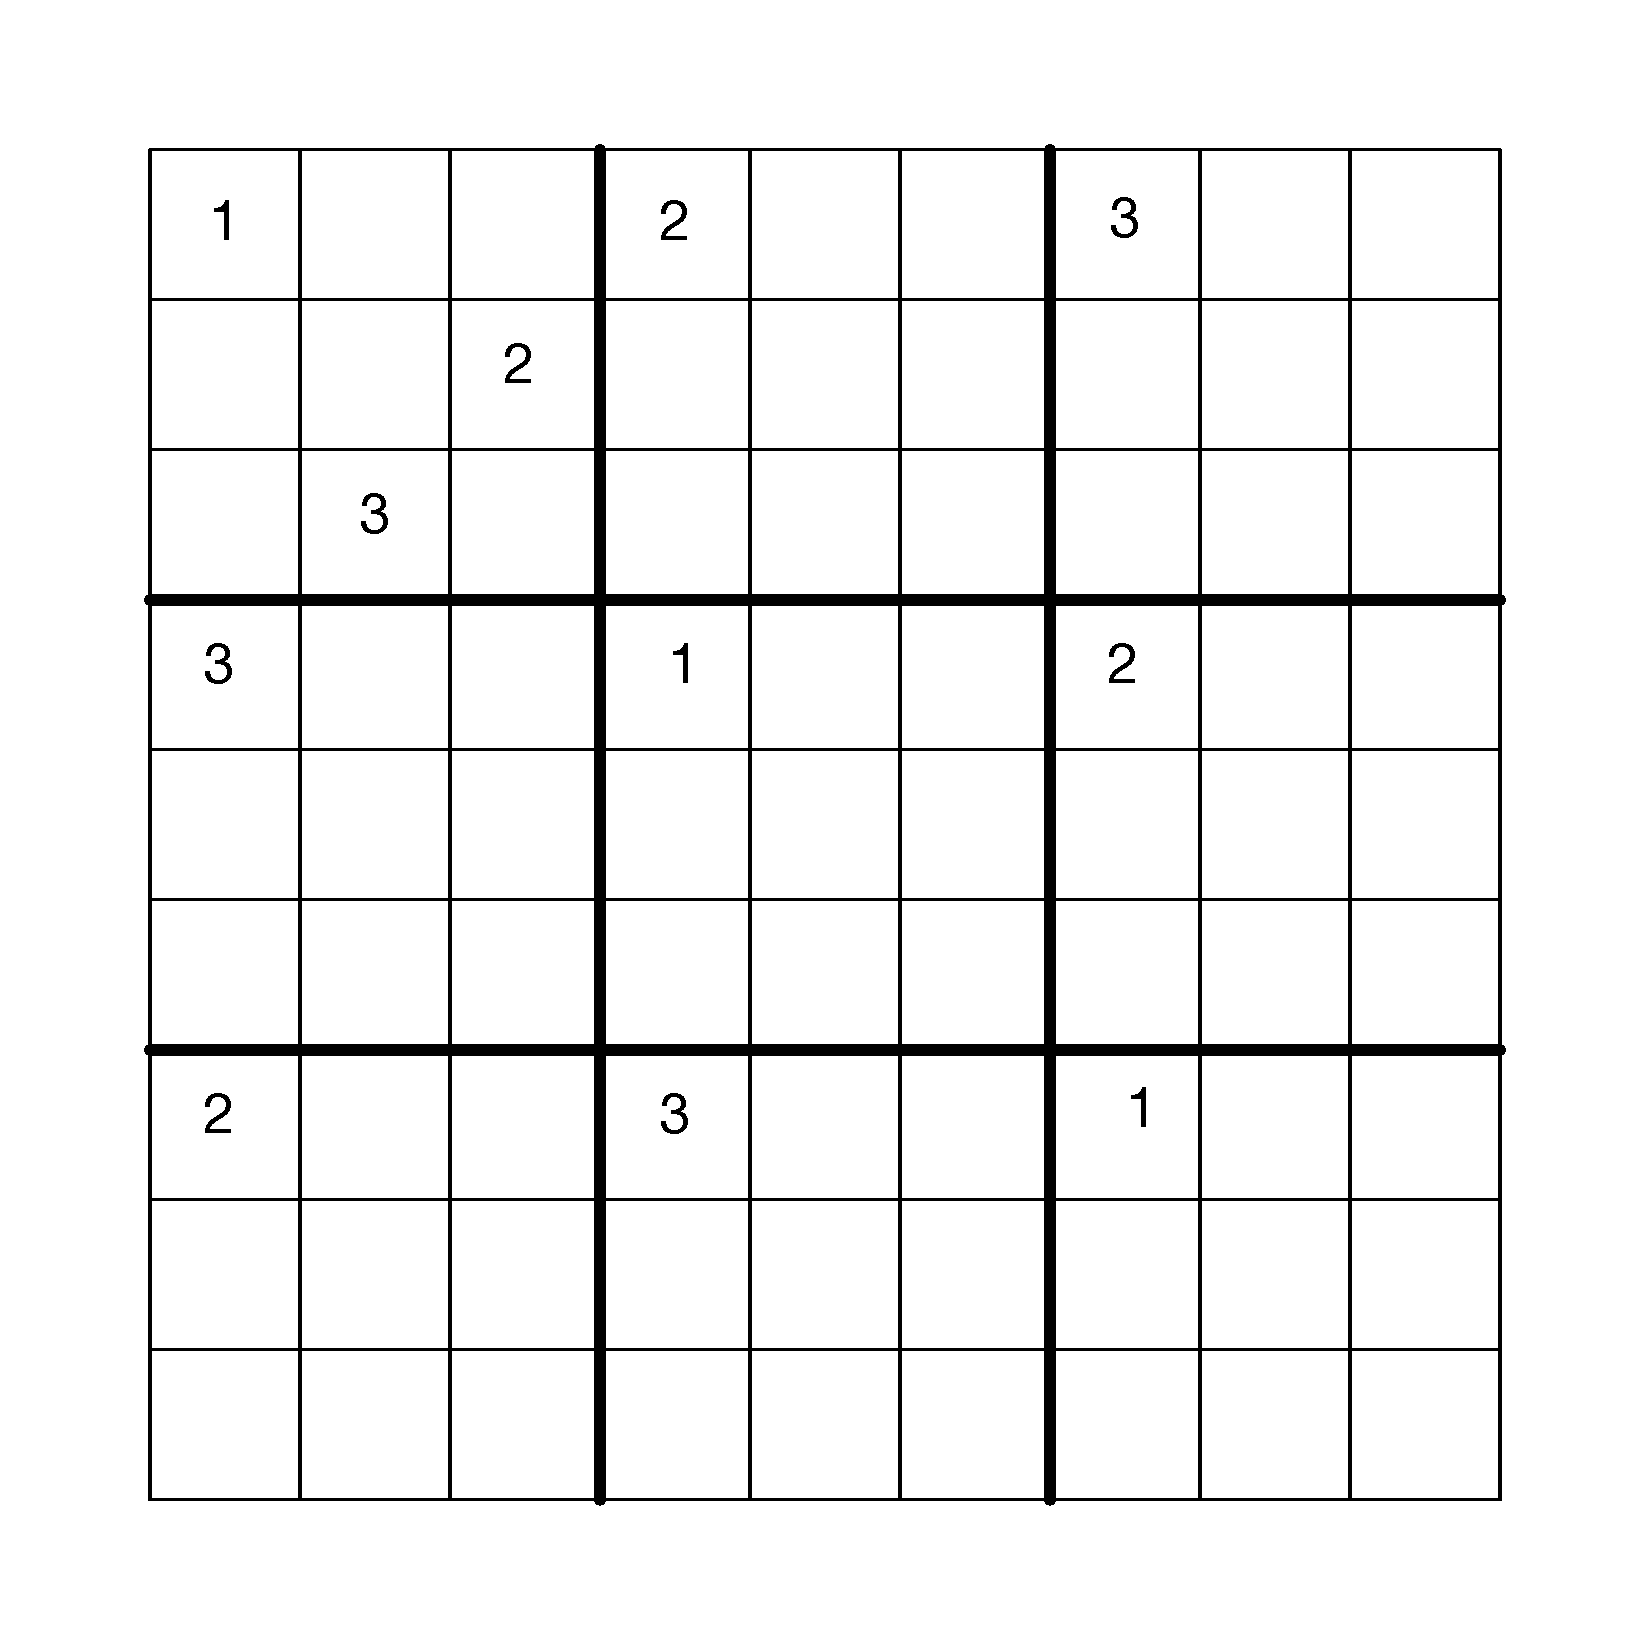
\includegraphics[width=0.45\textwidth]{figs/sudoku}
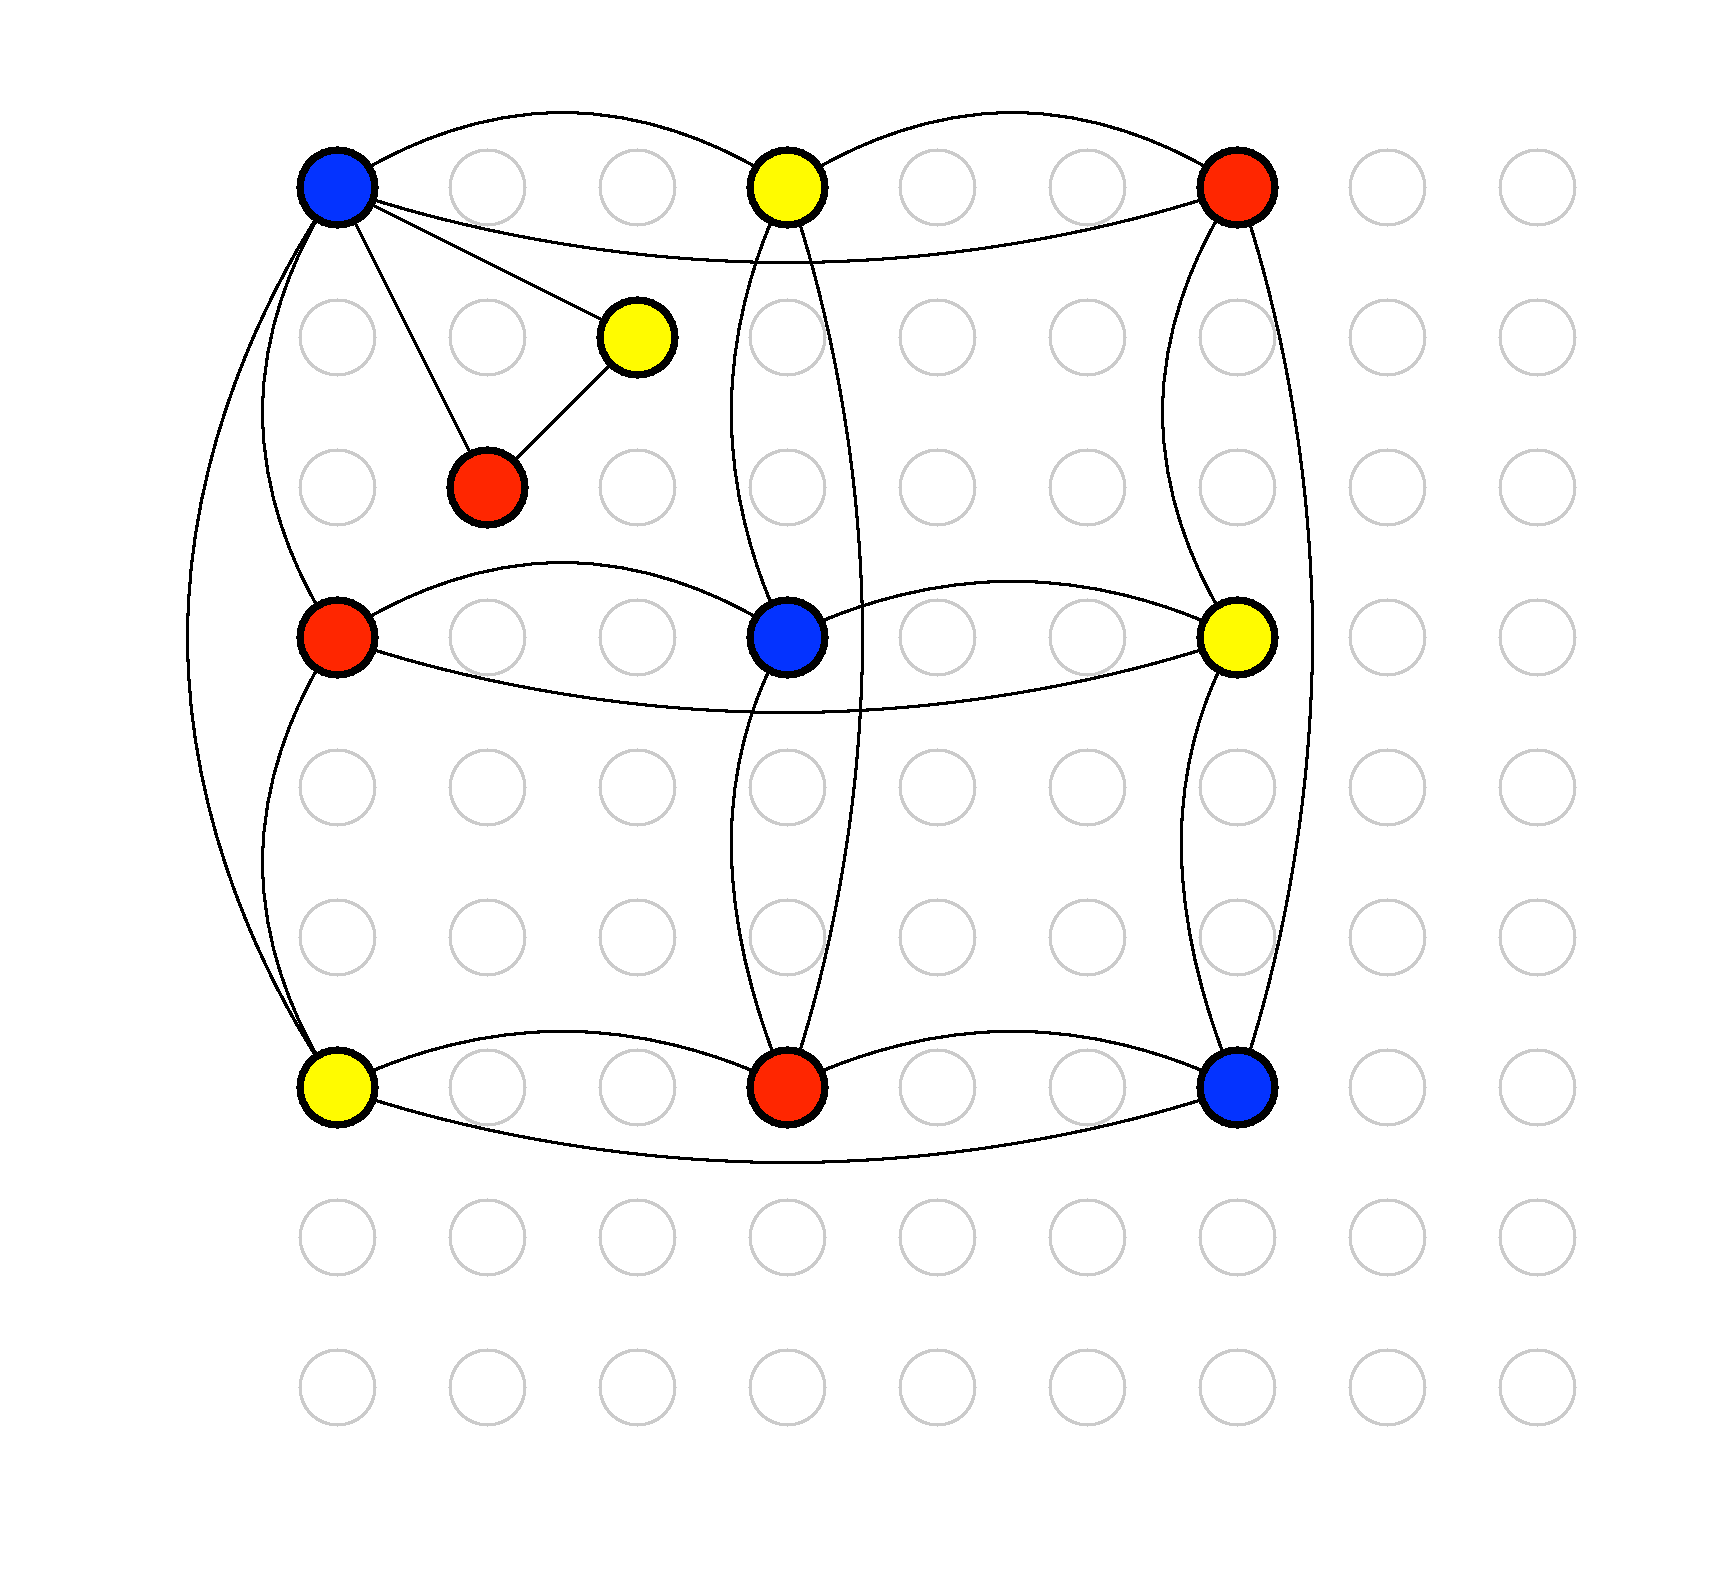
\includegraphics[width=0.5\textwidth]{figs/sudoku-graph}
\caption{A Sudoku game board and the corresponding colored graph.}
\label{fig:sudoku-graph}
\end{figure}


Given that Sudoku is an instance of graph coloring, one can use Sudoku
strategies to come up with an algorithm for allocating registers. For
example, one of the basic techniques for Sudoku is called Pencil
Marks. The idea is to use a process of elimination to determine what
numbers no longer make sense for a square and write down those
numbers in the square (writing very small). For example, if the number
$1$ is assigned to a square, then by process of elimination, you can
write the pencil mark $1$ in all the squares in the same row, column,
and region. Many Sudoku computer games provide automatic support for
Pencil Marks.
%
The Pencil Marks technique corresponds to the notion of
\emph{saturation}\index{saturation} due to \cite{Brelaz:1979eu}.
The saturation of a
vertex, in Sudoku terms, is the set of numbers that are no longer
available. In graph terminology, we have the following definition:
\begin{equation*}
  \mathrm{saturation}(u) = \{ c \;|\; \exists v. v \in \mathrm{neighbors}(u)
     \text{ and } \mathrm{color}(v) = c \}
\end{equation*}
where $\mathrm{neighbors}(u)$ is the set of vertices that share an
edge with $u$.

Using the Pencil Marks technique leads to a simple strategy for
filling in numbers: if there is a square with only one possible number
left, then choose that number! But what if there are no squares with
only one possibility left? One brute-force approach is to try them
all: choose the first  and if it ultimately leads to a solution,
great.  If not, backtrack and choose the next possibility.  One good
thing about Pencil Marks is that it reduces the degree of branching in
the search tree. Nevertheless, backtracking can be horribly time
consuming. One way to reduce the amount of backtracking is to use the
most-constrained-first heuristic. That is, when choosing a square,
always choose one with the fewest possibilities left (the vertex with
the highest saturation).  The idea is that choosing highly constrained
squares earlier rather than later is better because later on there may
not be any possibilities left for those squares.

However, register allocation is easier than Sudoku because the
register allocator can map variables to stack locations when the
registers run out. Thus, it makes sense to drop backtracking in favor
of greedy search, that is, make the best choice at the time and keep
going. We still wish to minimize the number of colors needed, so
keeping the most-constrained-first heuristic is a good idea.
Figure~\ref{fig:satur-algo} gives the pseudo-code for a simple greedy
algorithm for register allocation based on saturation and the
most-constrained-first heuristic. It is roughly equivalent to the
DSATUR algorithm of \cite{Brelaz:1979eu} (also known as saturation
degree ordering~\citep{Gebremedhin:1999fk,Omari:2006uq}).  Just as in
Sudoku, the algorithm represents colors with integers. The integers
$0$ through $k-1$ correspond to the $k$ registers that we use for
register allocation. The integers $k$ and larger correspond to stack
locations. The registers that are not used for register allocation,
such as \code{rax}, are assigned to negative integers. In particular,
we assign $-1$ to \code{rax}.

\begin{figure}[btp]
  \centering
\begin{lstlisting}[basicstyle=\rmfamily,deletekeywords={for,from,with,is,not,in,find},morekeywords={while},columns=fullflexible]
Algorithm: DSATUR
Input: a graph |$G$|
Output: an assignment |$\mathrm{color}[v]$| for each vertex |$v \in G$|

|$W \gets \mathrm{vertices}(G)$|
while |$W \neq \emptyset$| do
    pick a vertex |$u$| from |$W$| with the highest saturation,
        breaking ties randomly
    find the lowest color |$c$| that is not in |$\{ \mathrm{color}[v] \;:\; v \in \mathrm{adjacent}(u)\}$|
    |$\mathrm{color}[u] \gets c$|
    |$W \gets W - \{u\}$|
\end{lstlisting}
  \caption{The saturation-based greedy graph coloring algorithm.}
  \label{fig:satur-algo}
\end{figure}

With this algorithm in hand, let us return to the running example and
consider how to color the interference graph in
Figure~\ref{fig:interfere}.
%
We color the vertices for registers with their own color. For example,
\code{rax} is assigned the color $-1$.  We then update the saturation
for their neighboring vertices.  In this case, the saturation for
\code{t} includes $-1$.  The remaining vertices are not yet colored,
so they annotated with a dash, and their saturation sets are empty.
\[
\begin{tikzpicture}[baseline=(current  bounding  box.center)]
\node (rax) at (0,0) {$\ttm{rax}:-1,\{\}$};
\node (t1) at (0,2) {$\ttm{t}:-,\{-1\}$};
\node (z) at (3,2)  {$\ttm{z}:-,\{\}$};
\node (x) at (6,2)  {$\ttm{x}:-,\{\}$};
\node (y) at (3,0)  {$\ttm{y}:-,\{\}$};
\node (w) at (6,0)  {$\ttm{w}:-,\{\}$};
\node (v) at (9,0)  {$\ttm{v}:-,\{\}$};

\draw (t1) to (rax);
\draw (t1) to (z);
\draw (z) to (y);
\draw (z) to (w);
\draw (x) to (w);
\draw (y) to (w);
\draw (v) to (w);
\end{tikzpicture}
\]
The algorithm says to select a maximally saturated vertex. So we pick
$\ttm{t}$ and color it with the first available integer, which is
$0$. We mark $0$ as no longer available for $\ttm{z}$ and $\ttm{rax}$
because they interfere with $\ttm{t}$.
\[
\begin{tikzpicture}[baseline=(current  bounding  box.center)]
\node (rax) at (0,0) {$\ttm{rax}:-1,\{0\}$};
\node (t1) at (0,2) {$\ttm{t}:0,\{-1\}$};
\node (z) at (3,2)  {$\ttm{z}:-,\{0\}$};
\node (x) at (6,2)  {$\ttm{x}:-,\{\}$};
\node (y) at (3,0)  {$\ttm{y}:-,\{\}$};
\node (w) at (6,0)  {$\ttm{w}:-,\{\}$};
\node (v) at (9,0)  {$\ttm{v}:-,\{\}$};

\draw (t1) to (rax);
\draw (t1) to (z);
\draw (z) to (y);
\draw (z) to (w);
\draw (x) to (w);
\draw (y) to (w);
\draw (v) to (w);
\end{tikzpicture}
\]
We repeat the process, selecting another maximally saturated
vertex, which is \code{z}, and color it with the first available
number, which is $1$. We add $1$ to the saturations for the
neighboring vertices \code{t}, \code{y}, and \code{w}.
\[
\begin{tikzpicture}[baseline=(current  bounding  box.center)]
\node (rax) at (0,0) {$\ttm{rax}:-1,\{0\}$};
\node (t1) at (0,2) {$\ttm{t}:0,\{-1,1\}$};
\node (z) at (3,2)  {$\ttm{z}:1,\{0\}$};
\node (x) at (6,2)  {$\ttm{x}:-,\{\}$};
\node (y) at (3,0)  {$\ttm{y}:-,\{1\}$};
\node (w) at (6,0)  {$\ttm{w}:-,\{1\}$};
\node (v) at (9,0)  {$\ttm{v}:-,\{\}$};

\draw (t1) to (rax);
\draw (t1) to (z);
\draw (z) to (y);
\draw (z) to (w);
\draw (x) to (w);
\draw (y) to (w);
\draw (v) to (w);
\end{tikzpicture}
\]
The most saturated vertices are now \code{w} and \code{y}. We color
\code{w} with the first available color, which is $0$.
\[
\begin{tikzpicture}[baseline=(current  bounding  box.center)]
\node (rax) at (0,0) {$\ttm{rax}:-1,\{0\}$};
\node (t1) at (0,2) {$\ttm{t}:0,\{-1,1\}$};
\node (z) at (3,2)  {$\ttm{z}:1,\{0\}$};
\node (x) at (6,2)  {$\ttm{x}:-,\{0\}$};
\node (y) at (3,0)  {$\ttm{y}:-,\{0,1\}$};
\node (w) at (6,0)  {$\ttm{w}:0,\{1\}$};
\node (v) at (9,0)  {$\ttm{v}:-,\{0\}$};

\draw (t1) to (rax);
\draw (t1) to (z);
\draw (z) to (y);
\draw (z) to (w);
\draw (x) to (w);
\draw (y) to (w);
\draw (v) to (w);
\end{tikzpicture}
\]
Vertex \code{y} is now the most highly saturated, so we color \code{y}
with $2$.  We cannot choose $0$ or $1$ because those numbers are in
\code{y}'s saturation set. Indeed, \code{y} interferes with \code{w}
and \code{z}, whose colors are $0$ and $1$ respectively.
\[
\begin{tikzpicture}[baseline=(current  bounding  box.center)]
\node (rax) at (0,0) {$\ttm{rax}:-1,\{0\}$};
\node (t1) at (0,2) {$\ttm{t}:0,\{-1,1\}$};
\node (z) at (3,2)  {$\ttm{z}:1,\{0,2\}$};
\node (x) at (6,2)  {$\ttm{x}:-,\{0\}$};
\node (y) at (3,0)  {$\ttm{y}:2,\{0,1\}$};
\node (w) at (6,0)  {$\ttm{w}:0,\{1,2\}$};
\node (v) at (9,0)  {$\ttm{v}:-,\{0\}$};

\draw (t1) to (rax);
\draw (t1) to (z);
\draw (z) to (y);
\draw (z) to (w);
\draw (x) to (w);
\draw (y) to (w);
\draw (v) to (w);
\end{tikzpicture}
\]
Now \code{x} and \code{v} are the most saturated, so we color \code{v} it $1$.
\[
\begin{tikzpicture}[baseline=(current  bounding  box.center)]
\node (rax) at (0,0) {$\ttm{rax}:-1,\{0\}$};
\node (t1) at (0,2) {$\ttm{t}:0,\{-1,1\}$};
\node (z) at (3,2)  {$\ttm{z}:1,\{0,2\}$};
\node (x) at (6,2)  {$\ttm{x}:-,\{0\}$};
\node (y) at (3,0)  {$\ttm{y}:2,\{0,1\}$};
\node (w) at (6,0)  {$\ttm{w}:0,\{1,2\}$};
\node (v) at (9,0)  {$\ttm{v}:1,\{0\}$};

\draw (t1) to (rax);
\draw (t1) to (z);
\draw (z) to (y);
\draw (z) to (w);
\draw (x) to (w);
\draw (y) to (w);
\draw (v) to (w);
\end{tikzpicture}
\]
In the last step of the algorithm, we color \code{x} with $1$.
\[
\begin{tikzpicture}[baseline=(current  bounding  box.center)]
\node (rax) at (0,0) {$\ttm{rax}:-1,\{0\}$};
\node (t1) at (0,2) {$\ttm{t}:0,\{-1,1,\}$};
\node (z) at (3,2)  {$\ttm{z}:1,\{0,2\}$};
\node (x) at (6,2)  {$\ttm{x}:1,\{0\}$};
\node (y) at (3,0)  {$\ttm{y}:2,\{0,1\}$};
\node (w) at (6,0)  {$\ttm{w}:0,\{1,2\}$};
\node (v) at (9,0)  {$\ttm{v}:1,\{0\}$};

\draw (t1) to (rax);
\draw (t1) to (z);
\draw (z) to (y);
\draw (z) to (w);
\draw (x) to (w);
\draw (y) to (w);
\draw (v) to (w);
\end{tikzpicture}
\]

With the coloring complete, we finalize the assignment of variables to
registers and stack locations. Recall that if we have $k$ registers to
use for allocation, we map the first $k$ colors to registers and the
rest to stack locations.  Suppose for the moment that we have just one
register to use for register allocation, \key{rcx}. Then the following
is the mapping of colors to registers and stack allocations.
\[
  \{ 0 \mapsto \key{\%rcx}, \; 1 \mapsto \key{-8(\%rbp)}, \; 2 \mapsto \key{-16(\%rbp)} \}
\]
Putting this mapping together with the above coloring of the
variables, we arrive at the following assignment of variables to
registers and stack locations.
\begin{gather*}
  \{ \ttm{v} \mapsto \key{\%rcx}, \,
     \ttm{w} \mapsto \key{\%rcx},  \,
     \ttm{x} \mapsto \key{-8(\%rbp)}, \,
     \ttm{y} \mapsto \key{-16(\%rbp)}, \\
     \ttm{z} \mapsto \key{-8(\%rbp)}, \,
     \ttm{t} \mapsto \key{\%rcx} \}
\end{gather*}
Applying this assignment to our running example, on the left, yields
the program on the right.
% why frame size of 32? -JGS
\begin{center}
  \begin{minipage}{0.3\textwidth}
\begin{lstlisting}
movq $1, v
movq $42, w
movq v, x
addq $7, x
movq x, y
movq x, z
addq w, z
movq y, t
negq t
movq z, %rax
addq t, %rax
jmp conclusion
\end{lstlisting}
\end{minipage}
$\Rightarrow\qquad$
\begin{minipage}{0.45\textwidth}
\begin{lstlisting}
movq $1, %rcx
movq $42, %rcx
movq %rcx, -8(%rbp)
addq $7, -8(%rbp)
movq -8(%rbp), -16(%rbp)
movq -8(%rbp), -8(%rbp)
addq %rcx, -8(%rbp)
movq -16(%rbp), %rcx
negq %rcx
movq -8(%rbp), %rax
addq %rcx, %rax
jmp conclusion
\end{lstlisting}
\end{minipage}
\end{center}

The resulting program is almost an x86 program. The remaining step is
the patch instructions pass. In this example, the trivial move of
\code{-8(\%rbp)} to itself is deleted and the addition of
\code{-8(\%rbp)} to \key{-16(\%rbp)} is fixed by going through
\code{rax} as follows.
\begin{lstlisting}
movq -8(%rbp), %rax
addq %rax, -16(%rbp)
\end{lstlisting}

An overview of all of the passes involved in register allocation is
shown in Figure~\ref{fig:reg-alloc-passes}.

\begin{figure}[tbp]
\begin{tikzpicture}[baseline=(current  bounding  box.center)]
\node (R1) at (0,2)  {\large $R_1$};
\node (R1-2) at (3,2)  {\large $R_1$};
\node (R1-3) at (6,2)  {\large $R_1$};
\node (C0-1) at (3,0)  {\large $C_0$};

\node (x86-2) at (3,-2)  {\large $\text{x86}^{*}$};
\node (x86-3) at (6,-2)  {\large $\text{x86}^{*}$};
\node (x86-4) at (9,-2) {\large $\text{x86}$};
\node (x86-5) at (9,-4) {\large $\text{x86}^{\dagger}$};

\node (x86-2-1) at (3,-4)  {\large $\text{x86}^{*}$};
\node (x86-2-2) at (6,-4)  {\large $\text{x86}^{*}$};

\path[->,bend left=15] (R1) edge [above] node {\ttfamily\footnotesize uniquify} (R1-2);
\path[->,bend left=15] (R1-2) edge [above] node {\ttfamily\footnotesize remove-complex.} (R1-3);
\path[->,bend left=15] (R1-3) edge [right] node {\ttfamily\footnotesize explicate-control} (C0-1);
\path[->,bend right=15] (C0-1) edge [left] node {\ttfamily\footnotesize select-instr.} (x86-2);
\path[->,bend left=15] (x86-2) edge [right] node {\ttfamily\footnotesize\color{red} uncover-live} (x86-2-1);
\path[->,bend right=15] (x86-2-1) edge [below] node {\ttfamily\footnotesize\color{red} build-inter.} (x86-2-2);
\path[->,bend right=15] (x86-2-2) edge [right] node {\ttfamily\footnotesize\color{red} allocate-reg.} (x86-3);
\path[->,bend left=15] (x86-3) edge [above] node {\ttfamily\footnotesize patch-instr.} (x86-4);
\path[->,bend left=15] (x86-4) edge [right] node {\ttfamily\footnotesize print-x86} (x86-5);
\end{tikzpicture}
\caption{Diagram of the passes for $R_1$ with register allocation.}
\label{fig:reg-alloc-passes}
\end{figure}

\begin{wrapfigure}[24]{r}[1.0in]{0.6\textwidth}
  \small
  \begin{tcolorbox}[title=Priority Queue]
    A \emph{priority queue} is a collection of items in which the
    removal of items is governed by priority. In a ``min'' queue,
    lower priority items are removed first. An implementation is in
    \code{priority\_queue.rkt} of the support code.  \index{priority
      queue} \index{minimum priority queue}
  \begin{description}
  \item[$\LP\code{make-pqueue}\,\itm{cmp}\RP$] constructs an empty
    priority queue that uses the $\itm{cmp}$ predicate to determine
    whether its first argument has lower or equal priority to its
    second argument.
  \item[$\LP\code{pqueue-count}\,\itm{queue}\RP$] returns the number of
    items in the queue.
  \item[$\LP\code{pqueue-push!}\,\itm{queue}\,\itm{item}\RP$] inserts
    the item into the queue and returns a handle for the item in the
    queue.
  \item[$\LP\code{pqueue-pop!}\,\itm{queue}\RP$] returns the item with
    the lowest priority.
  \item[$\LP\code{pqueue-decrease-key!}\,\itm{queue}\,\itm{handle}\RP$]
    notifices the queue the the priority has decreased for the item
    associated with the given handle.
  \end{description}
\end{tcolorbox}
\end{wrapfigure}

We recommend creating a helper function named \code{color-graph} that
takes an interference graph and a list of all the variables in the
program. This function should return a mapping of variables to their
colors (represented as natural numbers). By creating this helper
function, you will be able to reuse it in Chapter~\ref{ch:functions}
when you add support for functions.  To prioritize the process of
highly saturated nodes inside your \code{color-graph} function, we
recommend using the priority queue data structure (see the side bar on
the right). Note that you will also need to maintain a mapping from
variables to their ``handles'' in the priority queue so that you can
notify the priority queue when their saturation changes.

Once you have obtained the coloring from \code{color-graph}, you can
assign the variables to registers or stack locations and then reuse
code from the \code{assign-homes} pass from
Section~\ref{sec:assign-r1} to replace the variables with their
assigned location.

\begin{exercise}\normalfont
  Implement the compiler pass \code{allocate-registers}, which should come
  after the \code{build-interference} pass. The three new passes,
  \code{uncover-live}, \code{build-interference}, and
  \code{allocate-registers} replace the \code{assign-homes} pass of
  Section~\ref{sec:assign-r1}.
  
  Test your updated compiler by creating new example programs that
  exercise all of the register allocation algorithm, such as forcing
  variables to be spilled to the stack.
\end{exercise}


\section{Print x86 and Conventions for Registers}
\label{sec:print-x86-reg-alloc}
\index{calling conventions}
\index{prelude}\index{conclusion}

Recall that the \code{print-x86} pass generates the prelude and
conclusion instructions for the \code{main} function.
%
The prelude saved the values in \code{rbp} and \code{rsp} and the
conclusion returned those values to \code{rbp} and \code{rsp}.  The
reason for this is that our \code{main} function must adhere to the
x86 calling conventions that we described in
Section~\ref{sec:calling-conventions}.  Furthermore, if your register
allocator assigned variables to other callee-saved registers
(e.g. \code{rbx}, \code{r12}, etc.), then those variables must also be
saved to the stack in the prelude and restored in the conclusion.  The
simplest approach is to save and restore all of the callee-saved
registers. The more efficient approach is to keep track of which
callee-saved registers were used and only save and restore
them. Either way, make sure to take this use of stack space into
account when you are calculating the size of the frame and adjusting
the \code{rsp} in the prelude. Also, don't forget that the size of the
frame needs to be a multiple of 16 bytes!


\section{Challenge: Move Biasing}
\label{sec:move-biasing}
\index{move biasing}

This section describes an optional enhancement to register allocation
for those students who are looking for an extra challenge or who have
a deeper interest in register allocation.

We return to the running example, but we remove the supposition that
we only have one register to use. So we have the following mapping of
color numbers to registers.
\[
  \{ 0 \mapsto \key{\%rbx}, \; 1 \mapsto \key{\%rcx}, \; 2 \mapsto \key{\%rdx} \}
\]
Using the same assignment of variables to color numbers that was
produced by the register allocator described in the last section, we
get the following program.

\begin{minipage}{0.3\textwidth}
\begin{lstlisting}
movq $1, v
movq $42, w
movq v, x
addq $7, x
movq x, y
movq x, z
addq w, z
movq y, t
negq t
movq z, %rax
addq t, %rax
jmp conclusion
\end{lstlisting}
\end{minipage}
$\Rightarrow\qquad$
\begin{minipage}{0.45\textwidth}
\begin{lstlisting}
movq $1, %rcx
movq $42, $rbx
movq %rcx, %rcx
addq $7, %rcx
movq %rcx, %rdx
movq %rcx, %rcx
addq %rbx, %rcx
movq %rdx, %rbx
negq %rbx
movq %rcx, %rax
addq %rbx, %rax
jmp conclusion
\end{lstlisting}
\end{minipage}

In the above output code there are two \key{movq} instructions that
can be removed because their source and target are the same.  However,
if we had put \key{t}, \key{v}, \key{x}, and \key{y} into the same
register, we could instead remove three \key{movq} instructions.  We
can accomplish this by taking into account which variables appear in
\key{movq} instructions with which other variables.

We say that two variables $p$ and $q$ are \emph{move
  related}\index{move related} if they participate together in a
\key{movq} instruction, that is, \key{movq} $p$\key{,} $q$ or
\key{movq} $q$\key{,} $p$. When the register allocator chooses a color
for a variable, it should prefer a color that has already been used
for a move-related variable (assuming that they do not interfere). Of
course, this preference should not override the preference for
registers over stack locations. This preference should be used as a
tie breaker when choosing between registers or when choosing between
stack locations.

We recommend representing the move relationships in a graph, similar
to how we represented interference.  The following is the \emph{move
  graph} for our running example.
\[
\begin{tikzpicture}[baseline=(current  bounding  box.center)]
\node (rax) at (0,0) {$\ttm{rax}$};
\node (t) at (0,2) {$\ttm{t}$};
\node (z) at (3,2)  {$\ttm{z}$};
\node (x) at (6,2)  {$\ttm{x}$};
\node (y) at (3,0)  {$\ttm{y}$};
\node (w) at (6,0)  {$\ttm{w}$};
\node (v) at (9,0)  {$\ttm{v}$};

\draw (v) to (x);
\draw (x) to (y);
\draw (x) to (z);
\draw (y) to (t);
\end{tikzpicture}
\]

Now we replay the graph coloring, pausing to see the coloring of
\code{y}. Recall the following configuration. The most saturated vertices
were \code{w} and \code{y}.
\[
\begin{tikzpicture}[baseline=(current  bounding  box.center)]
\node (rax) at (0,0) {$\ttm{rax}:-1,\{0\}$};
\node (t1) at (0,2) {$\ttm{t}:0,\{1\}$};
\node (z) at (3,2)  {$\ttm{z}:1,\{0\}$};
\node (x) at (6,2)  {$\ttm{x}:-,\{\}$};
\node (y) at (3,0)  {$\ttm{y}:-,\{1\}$};
\node (w) at (6,0)  {$\ttm{w}:-,\{1\}$};
\node (v) at (9,0)  {$\ttm{v}:-,\{\}$};

\draw (t1) to (rax);
\draw (t1) to (z);
\draw (z) to (y);
\draw (z) to (w);
\draw (x) to (w);
\draw (y) to (w);
\draw (v) to (w);
\end{tikzpicture}
\]
%
Last time we chose to color \code{w} with $0$. But this time we see
that \code{w} is not move related to any vertex, but \code{y} is move
related to \code{t}.  So we choose to color \code{y} the same color,
$0$.
\[
\begin{tikzpicture}[baseline=(current  bounding  box.center)]
\node (rax) at (0,0) {$\ttm{rax}:-1,\{0\}$};
\node (t1) at (0,2) {$\ttm{t}:0,\{1\}$};
\node (z) at (3,2)  {$\ttm{z}:1,\{0\}$};
\node (x) at (6,2)  {$\ttm{x}:-,\{\}$};
\node (y) at (3,0)  {$\ttm{y}:0,\{1\}$};
\node (w) at (6,0)  {$\ttm{w}:-,\{0,1\}$};
\node (v) at (9,0)  {$\ttm{v}:-,\{\}$};

\draw (t1) to (rax);
\draw (t1) to (z);
\draw (z) to (y);
\draw (z) to (w);
\draw (x) to (w);
\draw (y) to (w);
\draw (v) to (w);
\end{tikzpicture}
\]
Now \code{w} is the most saturated, so we color it $2$.
\[
\begin{tikzpicture}[baseline=(current  bounding  box.center)]
\node (rax) at (0,0) {$\ttm{rax}:-1,\{0\}$};
\node (t1) at (0,2) {$\ttm{t}:0,\{1\}$};
\node (z) at (3,2)  {$\ttm{z}:1,\{0,2\}$};
\node (x) at (6,2)  {$\ttm{x}:-,\{2\}$};
\node (y) at (3,0)  {$\ttm{y}:0,\{1,2\}$};
\node (w) at (6,0)  {$\ttm{w}:2,\{0,1\}$};
\node (v) at (9,0)  {$\ttm{v}:-,\{2\}$};

\draw (t1) to (rax);
\draw (t1) to (z);
\draw (z) to (y);
\draw (z) to (w);
\draw (x) to (w);
\draw (y) to (w);
\draw (v) to (w);
\end{tikzpicture}
\]
At this point, vertices \code{x} and \code{v} are most saturated, but
\code{x} is move related to \code{y} and \code{z}, so we color
\code{x} to $0$ to match \code{y}. Finally, we color \code{v} to $0$.
\[
\begin{tikzpicture}[baseline=(current  bounding  box.center)]
\node (rax) at (0,0) {$\ttm{rax}:-1,\{0\}$};
\node (t) at (0,2) {$\ttm{t}:0,\{1\}$};
\node (z) at (3,2)  {$\ttm{z}:1,\{0,2\}$};
\node (x) at (6,2)  {$\ttm{x}:0,\{2\}$};
\node (y) at (3,0)  {$\ttm{y}:0,\{1,2\}$};
\node (w) at (6,0)  {$\ttm{w}:2,\{0,1\}$};
\node (v) at (9,0)  {$\ttm{v}:0,\{2\}$};

\draw (t1) to (rax);
\draw (t) to (z);
\draw (z) to (y);
\draw (z) to (w);
\draw (x) to (w);
\draw (y) to (w);
\draw (v) to (w);
\end{tikzpicture}
\]

So we have the following assignment of variables to registers.
\begin{gather*}
  \{ \ttm{v} \mapsto \key{\%rbx}, \,
     \ttm{w} \mapsto \key{\%rdx}, \,
     \ttm{x} \mapsto \key{\%rbx}, \,
     \ttm{y} \mapsto \key{\%rbx}, \,
     \ttm{z} \mapsto \key{\%rcx}, \,
     \ttm{t} \mapsto \key{\%rbx} \}
\end{gather*}

We apply this register assignment to the running example, on the left,
to obtain the code on right.

\begin{minipage}{0.3\textwidth}
\begin{lstlisting}
movq $1, v
movq $42, w
movq v, x
addq $7, x
movq x, y
movq x, z
addq w, z
movq y, t
negq t
movq z, %rax
addq t, %rax
jmp conclusion
\end{lstlisting}
\end{minipage}
$\Rightarrow\qquad$
\begin{minipage}{0.45\textwidth}
  \begin{lstlisting}
movq $1, %rbx
movq $42, %rdx
movq %rbx, %rbx
addq $7, %rbx
movq %rbx, %rbx
movq %rbx, %rcx
addq %rdx, %rcx
movq %rbx, %rbx
negq %rbx
movq %rcx, %rax
addq %rbx, %rax
jmp conclusion
\end{lstlisting}
\end{minipage}

The \code{patch-instructions} then removes the three trivial moves
from \key{rbx} to \key{rbx} to obtain the following result.

\begin{minipage}{0.45\textwidth}
\begin{lstlisting}
movq $1, %rbx
movq $42, %rdx
addq $7, %rbx
movq %rbx, %rcx
addq %rdx, %rcx
negq %rbx
movq %rcx, %rax
addq %rbx, %rax
jmp conclusion
\end{lstlisting}
\end{minipage}

\begin{exercise}\normalfont
Change your implementation of \code{allocate-registers} to take move
biasing into account. Make sure that your compiler still passes all of
the previous tests. Create two new tests that include at least one
opportunity for move biasing and visually inspect the output x86
programs to make sure that your move biasing is working properly.
\end{exercise}

\margincomment{\footnotesize To do: another neat challenge would be to do
  live range splitting~\citep{Cooper:1998ly}. \\ --Jeremy}

\section{Output of the Running Example}
\label{sec:reg-alloc-output}
\index{prelude}\index{conclusion}

Figure~\ref{fig:running-example-x86} shows the x86 code generated for
the running example (Figure~\ref{fig:reg-eg}) with register allocation
and move biasing. To demonstrate both the use of registers and the
stack, we have limited the register allocator to use just two
registers: \code{rbx} and \code{rcx}.  In the prelude of the
\code{main} function, we push \code{rbx} onto the stack because it is
a callee-saved register and it was assigned to variable by the
register allocator.  We substract \code{8} from the \code{rsp} at the
end of the prelude to reserve space for the one spilled variable.
After that subtraction, the \code{rsp} is aligned to 16 bytes.

Moving on the the \code{start} block, we see how the registers were
allocated. Variables \code{v}, \code{x}, and \code{y} were assigned to
\code{rbx} and variable \code{z} was assigned to \code{rcx}.  Variable
\code{w} was spilled to the stack location \code{-16(\%rbp)}.  Recall
that the prelude saved the callee-save register \code{rbx} onto the
stack. The spilled variables must be placed lower on the stack than
the saved callee-save registers, so in this case \code{w} is placed at
\code{-16(\%rbp)}.

In the \code{conclusion}, we undo the work that was done in the
prelude. We move the stack pointer up by \code{8} bytes (the room for
spilled variables), then we pop the old values of \code{rbx} and
\code{rbp} (callee-saved registers), and finish with \code{retq} to
return control to the operating system.

  
\begin{figure}[tbp]
  % s0_28.rkt
  % (use-minimal-set-of-registers! #t)
  % and only rbx rcx
% tmp 0 rbx
% z 1  rcx
% y 0  rbx
% w 2  16(%rbp)
% v 0  rbx
% x 0  rbx
\begin{lstlisting}
start:
	movq	$1, %rbx
	movq	$42, -16(%rbp)
	addq	$7, %rbx
	movq	%rbx, %rcx
	addq	-16(%rbp), %rcx
	negq	%rbx
	movq	%rcx, %rax
	addq	%rbx, %rax
	jmp conclusion

	.globl main
main:
	pushq	%rbp
	movq	%rsp, %rbp
	pushq	%rbx
	subq	$8, %rsp
	jmp start
        
conclusion:
	addq	$8, %rsp
	popq	%rbx
	popq	%rbp
	retq
\end{lstlisting}
\caption{The x86 output from the running example (Figure~\ref{fig:reg-eg}).}
\label{fig:running-example-x86}
\end{figure}



%%%%%%%%%%%%%%%%%%%%%%%%%%%%%%%%%%%%%%%%%%%%%%%%%%%%%%%%%%%%%%%%%%%%%%%%%%%%%%%%
\chapter{Booleans and Control Flow}
\label{ch:bool-types}
\index{Boolean}
\index{control flow}
\index{conditional expression}

The $R_0$ and $R_1$ languages only have a single kind of value, the
integers. In this chapter we add a second kind of value, the Booleans,
to create the $R_2$ language. The Boolean values \emph{true} and
\emph{false} are written \key{\#t} and \key{\#f} respectively in
Racket.  The $R_2$ language includes several operations that involve
Booleans (\key{and}, \key{not}, \key{eq?}, \key{<}, etc.) and the
conditional \key{if} expression. With the addition of \key{if}
expressions, programs can have non-trivial control flow which which
significantly impacts the \code{explicate-control} and the liveness
analysis for register allocation. Also, because we now have two kinds
of values, we need to handle programs that apply an operation to the
wrong kind of value, such as \code{(not 1)}.

There are two language design options for such situations.  One option
is to signal an error and the other is to provide a wider
interpretation of the operation. The Racket language uses a mixture of
these two options, depending on the operation and the kind of
value. For example, the result of \code{(not 1)} in Racket is
\code{\#f} because Racket treats non-zero integers as if they were
\code{\#t}. On the other hand, \code{(car 1)} results in a run-time
error in Racket stating that \code{car} expects a pair.

The Typed Racket language makes similar design choices as Racket,
except much of the error detection happens at compile time instead of
run time. Like Racket, Typed Racket accepts and runs \code{(not 1)},
producing \code{\#f}. But in the case of \code{(car 1)}, Typed Racket
reports a compile-time error because Typed Racket expects the type of
the argument to be of the form \code{(Listof T)} or \code{(Pairof T1 T2)}.

For the $R_2$ language we choose to be more like Typed Racket in that
we perform type checking during compilation. In
Chapter~\ref{ch:type-dynamic} we study the alternative choice, that
is, how to compile a dynamically typed language like Racket.  The
$R_2$ language is a subset of Typed Racket but by no means includes
all of Typed Racket. For many operations we take a narrower
interpretation than Typed Racket, for example, rejecting \code{(not 1)}.

This chapter is organized as follows.  We begin by defining the syntax
and interpreter for the $R_2$ language (Section~\ref{sec:r2-lang}). We
then introduce the idea of type checking and build a type checker for
$R_2$ (Section~\ref{sec:type-check-r2}). To compile $R_2$ we need to
enlarge the intermediate language $C_0$ into $C_1$, which we do in
Section~\ref{sec:c1}. The remaining sections of this chapter discuss
how our compiler passes need to change to accommodate Booleans and
conditional control flow.


\section{The $R_2$ Language}
\label{sec:r2-lang}

The concrete syntax of the $R_2$ language is defined in
Figure~\ref{fig:r2-concrete-syntax} and the abstract syntax is defined
in Figure~\ref{fig:r2-syntax}. The $R_2$ language includes all of
$R_1$ (shown in gray), the Boolean literals \code{\#t} and \code{\#f},
and the conditional \code{if} expression. Also, we expand the
operators to include
\begin{enumerate}
\item subtraction on integers,
\item the logical operators \key{and}, \key{or} and \key{not},
\item the \key{eq?} operation for comparing two integers or two Booleans, and
\item the \key{<}, \key{<=}, \key{>}, and \key{>=} operations for
  comparing integers.
\end{enumerate}

\begin{figure}[tp]
\centering
\fbox{
\begin{minipage}{0.96\textwidth}
\[
\begin{array}{lcl}
  \itm{bool} &::=& \key{\#t} \mid \key{\#f} \\  
  \itm{cmp} &::= & \key{eq?} \mid \key{<} \mid \key{<=} \mid \key{>} \mid \key{>=} \\
  \Exp &::=& \gray{ \Int \mid (\key{read}) \mid (\key{-}\;\Exp) \mid (\key{+} \; \Exp\;\Exp) }  \mid (\key{-}\;\Exp\;\Exp) \\
     &\mid&  \gray{ \Var \mid (\key{let}~([\Var~\Exp])~\Exp) } \\
     &\mid& \itm{bool}
      \mid (\key{and}\;\Exp\;\Exp) \mid (\key{or}\;\Exp\;\Exp)
      \mid (\key{not}\;\Exp) \\
      &\mid& (\itm{cmp}\;\Exp\;\Exp) \mid (\key{if}~\Exp~\Exp~\Exp) \\
  R_2 &::=& \Exp
\end{array}
\]
\end{minipage}
}
\caption{The concrete syntax of $R_2$, extending $R_1$
  (Figure~\ref{fig:r1-concrete-syntax}) with Booleans and conditionals.}
\label{fig:r2-concrete-syntax}
\end{figure}

\begin{figure}[tp]
\centering
\fbox{
\begin{minipage}{0.96\textwidth}
\[
\begin{array}{lcl}
  \itm{bool} &::=& \key{\#t} \mid \key{\#f} \\
  \itm{cmp} &::= & \key{eq?} \mid \key{<} \mid \key{<=} \mid \key{>} \mid \key{>=} \\
  \Exp &::=& \gray{ \INT{\Int} \mid \READ{} } \\
    &\mid& \gray{ \NEG{\Exp} \mid \ADD{\Exp}{\Exp} }\\
     &\mid& \BINOP{\code{'-}}{\Exp}{\Exp} \\
     &\mid& \gray{ \VAR{\Var} \mid \LET{\Var}{\Exp}{\Exp} } \\
     &\mid& \BOOL{\itm{bool}}  \mid \AND{\Exp}{\Exp}\\
     &\mid& \OR{\Exp}{\Exp} \mid \NOT{\Exp} \\
      &\mid& \BINOP{\itm{cmp}}{\Exp}{\Exp} \mid \IF{\Exp}{\Exp}{\Exp} \\
  R_2 &::=& \PROGRAM{\key{'()}}{\Exp}
\end{array}
\]
\end{minipage}
}
\caption{The abstract syntax of $R_2$.}
\label{fig:r2-syntax}
\end{figure}

Figure~\ref{fig:interp-R2} defines the interpreter for $R_2$, omitting
the parts that are the same as the interpreter for $R_1$
(Figure~\ref{fig:interp-R1}). The literals \code{\#t} and \code{\#f}
evaluate to the corresponding Boolean values. The conditional
expression $(\key{if}\, \itm{cnd}\,\itm{thn}\,\itm{els})$ evaluates
the Boolean expression \itm{cnd} and then either evaluates \itm{thn}
or \itm{els} depending on whether \itm{cnd} produced \code{\#t} or
\code{\#f}. The logical operations \code{not} and \code{and} behave as
you might expect, but note that the \code{and} operation is
short-circuiting. That is, given the expression
$(\key{and}\,e_1\,e_2)$, the expression $e_2$ is not evaluated if
$e_1$ evaluates to \code{\#f}.

With the addition of the comparison operations, there are quite a few
primitive operations and the interpreter code for them could become
repetitive without some care. In Figure~\ref{fig:interp-R2} we factor
out the different parts of the code for primitive operations into the
\code{interp-op} function and the similar parts of the code into the
match clause for \code{Prim} shown in Figure~\ref{fig:interp-R2}. We
do not use \code{interp-op} for the \code{and} operation because of
the short-circuiting behavior in the order of evaluation of its
arguments.


\begin{figure}[tbp]
\begin{lstlisting}
(define (interp-op op)
  (match op
    ...
    ['not (lambda (v) (match v [#t #f] [#f #t]))]
    ['eq? (lambda (v1 v2)
            (cond [(or (and (fixnum? v1) (fixnum? v2))
                       (and (boolean? v1) (boolean? v2)))
                   (eq? v1 v2)]))]
    ['< (lambda (v1 v2)
          (cond [(and (fixnum? v1) (fixnum? v2)) (< v1 v2)]))]
    ['<= (lambda (v1 v2)
           (cond [(and (fixnum? v1) (fixnum? v2)) (<= v1 v2)]))]
    ['> (lambda (v1 v2)
          (cond [(and (fixnum? v1) (fixnum? v2)) (> v1 v2)]))]
    ['>= (lambda (v1 v2)
           (cond [(and (fixnum? v1) (fixnum? v2)) (>= v1 v2)]))]
    [else (error 'interp-op "unknown operator")]))

(define (interp-exp env)
  (lambda (e)
    (define recur (interp-exp env))
    (match e
      ...
      [(Bool b) b]
      [(If cnd thn els)
       (define b (recur cnd))
       (match b
         [#t (recur thn)]
         [#f (recur els)])]
      [(Prim 'and (list e1 e2))
       (define v1 (recur e1))
       (match v1
         [#t (match (recur e2) [#t #t] [#f #f])]
         [#f #f])]
      [(Prim op args)
       (apply (interp-op op) (for/list ([e args]) (recur e)))]
      )))

(define (interp-R2 p)
  (match p
    [(Program info e)
     ((interp-exp '()) e)]
    ))
\end{lstlisting}
\caption{Interpreter for the $R_2$ language.}
\label{fig:interp-R2}
\end{figure}


\section{Type Checking $R_2$ Programs}
\label{sec:type-check-r2}
\index{type checking}
\index{semantic analysis}

It is helpful to think about type checking in two complementary
ways. A type checker predicts the type of value that will be produced
by each expression in the program.  For $R_2$, we have just two types,
\key{Integer} and \key{Boolean}. So a type checker should predict that
\begin{lstlisting}
   (+ 10 (- (+ 12 20)))
\end{lstlisting}
produces an \key{Integer} while
\begin{lstlisting}
   (and (not #f) #t)
\end{lstlisting}
produces a \key{Boolean}.

Another way to think about type checking is that it enforces a set of
rules about which operators can be applied to which kinds of
values. For example, our type checker for $R_2$ will signal an error
for the below expression because, as we have seen above, the
expression \code{(+ 10 ...)} has type \key{Integer} but the type
checker enforces the rule that the argument of \code{not} must be a
\key{Boolean}.
\begin{lstlisting}
   (not (+ 10 (- (+ 12 20))))
\end{lstlisting}

The type checker for $R_2$ is a structurally recursive function over
the AST. Figure~\ref{fig:type-check-R2} shows many of the clauses for
the \code{type-check-exp} function.  Given an input expression
\code{e}, the type checker either returns a type (\key{Integer} or
\key{Boolean}) or it signals an error.  The type of an integer literal
is \code{Integer} and the type of a Boolean literal is \code{Boolean}.
To handle variables, the type checker uses an environment that maps
variables to types. Consider the clause for \key{let}.  We type check
the initializing expression to obtain its type \key{T} and then
associate type \code{T} with the variable \code{x} in the
environment. When the type checker encounters a use of variable
\code{x} in the body of the \key{let}, it can find its type in the
environment.

\begin{figure}[tbp]
\begin{lstlisting}
(define (type-check-exp env)
  (lambda (e)
    (match e
      [(Var x) (dict-ref env x)]
      [(Int n) 'Integer]
      [(Bool b) 'Boolean]
      [(Let x e body)
        (define Te ((type-check-exp env) e))
        (define Tb ((type-check-exp (dict-set env x Te)) body))
        Tb]
      ...
      [else
       (error "type-check-exp couldn't match" e)])))

(define (type-check env)
  (lambda (e)
    (match e
      [(Program info body)
       (define Tb ((type-check-exp '()) body))
       (unless (equal? Tb 'Integer)
         (error "result of the program must be an integer, not " Tb))
       (Program info body)]
      )))
\end{lstlisting}
\caption{Skeleton of a type checker for the $R_2$ language.}
\label{fig:type-check-R2}
\end{figure}

\begin{exercise}\normalfont
Complete the implementation of \code{type-check}.  Test your type
checker using \code{interp-tests} and \code{compiler-tests} by passing
the \code{type-check} function as the second argument.  Create 10 new
example programs in $R_2$ that you choose based on how thoroughly they
test you type checking function. Half of the example programs should
have a type error to make sure that your type checker properly rejects
them. For those programs, to signal that a type error is expected,
create an empty file with the same base name but with file extension
\code{.tyerr}. For example, if the test \code{r2\_14.rkt} is expected
to error, then create an empty file named \code{r2\_14.tyerr}.  The
other half of the example programs should not have type errors. Note
that if your type checker does not signal an error for a program, then
interpreting that program should not encounter an error.  If it does,
there is something wrong with your type checker.
\end{exercise}


\section{Shrink the $R_2$ Language}
\label{sec:shrink-r2}

The $R_2$ language includes several operators that are easily
expressible in terms of other operators. For example, subtraction is
expressible in terms of addition and negation.
\[
 \key{(-}\; e_1 \; e_2\key{)} \quad \Rightarrow \quad \LP\key{+} \; e_1 \; \LP\key{-} \; e_2\RP\RP
\]
Several of the comparison operations are expressible in terms of
less-than and logical negation.
\[
\LP\key{<=}\; e_1 \; e_2\RP \quad \Rightarrow \quad
\LP\key{let}~\LP\LS\key{tmp.1}~e_1\RS\RP~\LP\key{not}\;\LP\key{<}\;e_2\;\key{tmp.1})\RP\RP
\]
The \key{let} is needed in the above translation to ensure that
expression $e_1$ is evaluated before $e_2$.

By performing these translations near the front-end of the compiler,
the later passes of the compiler do not need to deal with these
constructs, making those passes shorter. On the other hand, sometimes
these translations make it more difficult to generate the most
efficient code with respect to the number of instructions. However,
these differences typically do not affect the number of accesses to
memory, which is the primary factor that determines execution time on
modern computer architectures.

\begin{exercise}\normalfont
  Implement the pass \code{shrink} that removes subtraction,
  \key{and}, \key{or}, \key{<=}, \key{>}, and \key{>=} from the language
  by translating them to other constructs in $R_2$.  Create tests to
  make sure that the behavior of all of these constructs stays the
  same after translation.
\end{exercise}


\section{The x86$_1$ Language}
\label{sec:x86-1}

\index{x86}
To implement the new logical operations, the comparison operations,
and the \key{if} expression, we need to delve further into the x86
language. Figures~\ref{fig:x86-1-concrete} and \ref{fig:x86-1} define
the concrete and abstract syntax for a larger subset of x86 that
includes instructions for logical operations, comparisons, and
conditional jumps.

One small challenge is that x86 does not provide an instruction that
directly implements logical negation (\code{not} in $R_2$ and $C_1$).
However, the \code{xorq} instruction can be used to encode \code{not}.
The \key{xorq} instruction takes two arguments, performs a pairwise
exclusive-or ($\mathrm{XOR}$) operation on each bit of its arguments,
and writes the results into its second argument.  Recall the truth
table for exclusive-or:
\begin{center}
\begin{tabular}{l|cc}
   & 0 & 1 \\ \hline
0  & 0 & 1 \\
1  & 1 & 0
\end{tabular}
\end{center}
For example, applying $\mathrm{XOR}$ to each bit of the binary numbers
$0011$ and $0101$ yields $0110$. Notice that in the row of the table
for the bit $1$, the result is the opposite of the second bit.  Thus,
the \code{not} operation can be implemented by \code{xorq} with $1$ as
the first argument:
\[
\Var~ \key{=}~ \LP\key{not}~\Arg\RP\key{;}
\qquad\Rightarrow\qquad
\begin{array}{l}
\key{movq}~ \Arg\key{,} \Var\\
\key{xorq}~ \key{\$1,} \Var
\end{array}
\]


\begin{figure}[tp]
\fbox{
\begin{minipage}{0.96\textwidth}
\[
\begin{array}{lcl}
  \itm{bytereg} &::=& \key{ah} \mid \key{al} \mid \key{bh} \mid \key{bl}
    \mid \key{ch} \mid \key{cl} \mid \key{dh} \mid \key{dl} \\
\Arg &::=& \gray{ \key{\$}\Int \mid \key{\%}\Reg \mid \Int\key{(}\key{\%}\Reg\key{)} } \mid \key{\%}\itm{bytereg}\\
\itm{cc} & ::= & \key{e} \mid \key{l} \mid \key{le} \mid \key{g} \mid \key{ge} \\
\Instr &::=& \gray{ \key{addq} \; \Arg\key{,} \Arg \mid
      \key{subq} \; \Arg\key{,} \Arg \mid
      \key{negq} \; \Arg \mid \key{movq} \; \Arg\key{,} \Arg \mid } \\
  &&  \gray{ \key{callq} \; \itm{label} \mid
      \key{pushq}\;\Arg \mid \key{popq}\;\Arg \mid \key{retq} \mid \key{jmp}\,\itm{label} } \\
  && \gray{ \itm{label}\key{:}\; \Instr }
     \mid \key{xorq}~\Arg\key{,}~\Arg
     \mid \key{cmpq}~\Arg\key{,}~\Arg  \mid \\
  &&  \key{set}cc~\Arg
     \mid \key{movzbq}~\Arg\key{,}~\Arg
     \mid \key{j}cc~\itm{label}
     \\
x86_1 &::= & \gray{ \key{.globl main} }\\
      &    & \gray{ \key{main:} \; \Instr\ldots }
\end{array}
\]
\end{minipage}
}
\caption{The concrete syntax of x86$_1$  (extends x86$_0$ of Figure~\ref{fig:x86-0-concrete}).}
\label{fig:x86-1-concrete}
\end{figure}

\begin{figure}[tp]
\fbox{
\begin{minipage}{0.96\textwidth}
\small    
\[
\begin{array}{lcl}
\itm{bytereg} &::=& \key{ah} \mid \key{al} \mid \key{bh} \mid \key{bl}
    \mid \key{ch} \mid \key{cl} \mid \key{dh} \mid \key{dl} \\
\Arg &::=&  \gray{\IMM{\Int} \mid \REG{\Reg} \mid \DEREF{\Reg}{\Int}} 
     \mid \BYTEREG{\itm{bytereg}} \\
\itm{cc} & ::= & \key{e} \mid \key{l} \mid \key{le} \mid \key{g} \mid \key{ge} \\
\Instr &::=& \gray{ \BININSTR{\code{'addq}}{\Arg}{\Arg} 
       \mid \BININSTR{\code{'subq}}{\Arg}{\Arg} } \\
       &\mid& \gray{ \BININSTR{\code{'movq}}{\Arg}{\Arg} 
       \mid \UNIINSTR{\code{'negq}}{\Arg} } \\
       &\mid& \gray{ \CALLQ{\itm{label}}{\itm{int}} \mid \RETQ{} 
       \mid \PUSHQ{\Arg} \mid \POPQ{\Arg} \mid \JMP{\itm{label}} } \\
       &\mid& \BININSTR{\code{'xorq}}{\Arg}{\Arg}
       \mid \BININSTR{\code{'cmpq}}{\Arg}{\Arg}\\
       &\mid& \BININSTR{\code{'set}}{\itm{cc}}{\Arg} 
       \mid \BININSTR{\code{'movzbq}}{\Arg}{\Arg}\\
       &\mid&  \JMPIF{\itm{cc}}{\itm{label}} \\
\Block &::= & \gray{\BLOCK{\itm{info}}{\Instr\ldots}} \\
x86_1 &::= & \gray{\PROGRAM{\itm{info}}{\CFG{\key{(}\itm{label} \,\key{.}\, \Block \key{)}\ldots}}}
\end{array}
\]
\end{minipage}
}
\caption{The abstract syntax of x86$_1$ (extends x86$_0$ of Figure~\ref{fig:x86-0-ast}).}
\label{fig:x86-1}
\end{figure}

Next we consider the x86 instructions that are relevant for compiling
the comparison operations. The \key{cmpq} instruction compares its two
arguments to determine whether one argument is less than, equal, or
greater than the other argument. The \key{cmpq} instruction is unusual
regarding the order of its arguments and where the result is
placed. The argument order is backwards: if you want to test whether
$x < y$, then write \code{cmpq} $y$\code{,} $x$. The result of
\key{cmpq} is placed in the special EFLAGS register. This register
cannot be accessed directly but it can be queried by a number of
instructions, including the \key{set} instruction. The \key{set}
instruction puts a \key{1} or \key{0} into its destination depending
on whether the comparison came out according to the condition code
\itm{cc} (\key{e} for equal, \key{l} for less, \key{le} for
less-or-equal, \key{g} for greater, \key{ge} for greater-or-equal).
The \key{set} instruction has an annoying quirk in that its
destination argument must be single byte register, such as \code{al}
(L for lower bits) or \code{ah} (H for higher bits), which are part of
the \code{rax} register.  Thankfully, the \key{movzbq} instruction can
then be used to move from a single byte register to a normal 64-bit
register.

The x86 instruction for conditional jump are relevant to the
compilation of \key{if} expressions.  The \key{JmpIf} instruction
updates the program counter to point to the instruction after the
indicated label depending on whether the result in the EFLAGS register
matches the condition code \itm{cc}, otherwise the \key{JmpIf}
instruction falls through to the next instruction.  The abstract
syntax for \key{JmpIf} differs from the concrete syntax for x86 in
that it separates the instruction name from the condition code. For
example, \code{(JmpIf le foo)} corresponds to \code{jle foo}.  Because
the \key{JmpIf} instruction relies on the EFLAGS register, it is
common for the \key{JmpIf} to be immediately preceded by a \key{cmpq}
instruction to set the EFLAGS register.


\section{The $C_1$ Intermediate Language}
\label{sec:c1}

As with $R_1$, we compile $R_2$ to a C-like intermediate language, but
we need to grow that intermediate language to handle the new features
in $R_2$: Booleans and conditional expressions.
Figure~\ref{fig:c1-concrete-syntax} defines the concrete syntax of
$C_1$ and Figure~\ref{fig:c1-syntax} defines the abstract syntax.  In
particular, we add logical and comparison operators to the $\Exp$
non-terminal and the literals \key{\#t} and \key{\#f} to the $\Arg$
non-terminal.  Regarding control flow, $C_1$ differs considerably from
$R_2$.  Instead of \key{if} expressions, $C_1$ has \key{goto} and
conditional \key{goto} in the grammar for $\Tail$. This means that a
sequence of statements may now end with a \code{goto} or a conditional
\code{goto}. The conditional \code{goto} jumps to one of two labels
depending on the outcome of the comparison. In
Section~\ref{sec:explicate-control-r2} we discuss how to translate
from $R_2$ to $C_1$, bridging this gap between \key{if} expressions
and \key{goto}'s.

\begin{figure}[tbp]
\fbox{
\begin{minipage}{0.96\textwidth}
\small    
\[
\begin{array}{lcl}
\Atm &::=& \gray{ \Int \mid \Var } \mid \itm{bool} \\
\itm{cmp} &::= & \key{eq?} \mid \key{<}  \\
\Exp &::=& \gray{ \Atm \mid \key{(read)} \mid \key{(-}~\Atm\key{)} \mid \key{(+}~\Atm~\Atm\key{)} } \\
   &\mid& \LP \key{not}~\Atm \RP \mid \LP \itm{cmp}~\Atm~\Atm\RP \\
\Stmt &::=& \gray{ \Var~\key{=}~\Exp\key{;} } \\
\Tail &::= & \gray{ \key{return}~\Exp\key{;} \mid \Stmt~\Tail } 
   \mid \key{goto}~\itm{label}\key{;}\\
   &\mid& \key{if}~\LP \itm{cmp}~\Atm~\Atm \RP~ \key{goto}~\itm{label}\key{;} ~\key{else}~\key{goto}~\itm{label}\key{;} \\
C_1 & ::= & \gray{ (\itm{label}\key{:}~ \Tail)\ldots }
\end{array}
\]
\end{minipage}
}
\caption{The concrete syntax of the $C_1$ intermediate language.}
\label{fig:c1-concrete-syntax}
\end{figure}

\begin{figure}[tp]
\fbox{
\begin{minipage}{0.96\textwidth}
\small    
\[
\begin{array}{lcl}
\Atm &::=& \gray{\INT{\Int} \mid \VAR{\Var}} \mid \BOOL{\itm{bool}} \\
\itm{cmp} &::= & \key{eq?} \mid \key{<}  \\
\Exp &::= & \gray{ \Atm \mid \READ{} }\\
     &\mid& \gray{ \NEG{\Atm} \mid \ADD{\Atm}{\Atm} } \\
     &\mid& \UNIOP{\key{'not}}{\Atm} 
     \mid \BINOP{\key{'}\itm{cmp}}{\Atm}{\Atm} \\
\Stmt &::=& \gray{ \ASSIGN{\VAR{\Var}}{\Exp} } \\
\Tail &::= & \gray{\RETURN{\Exp} \mid \SEQ{\Stmt}{\Tail} } 
    \mid \GOTO{\itm{label}} \\
    &\mid& \IFSTMT{\BINOP{\itm{cmp}}{\Atm}{\Atm}}{\GOTO{\itm{label}}}{\GOTO{\itm{label}}} \\
C_1 & ::= & \gray{\PROGRAM{\itm{info}}{\CFG{\key{(}\itm{label}\,\key{.}\,\Tail\key{)}\ldots}}}
\end{array}
\]
\end{minipage}
}
\caption{The abstract syntax of $C_1$, an extention of $C_0$
  (Figure~\ref{fig:c0-syntax}).}
\label{fig:c1-syntax}
\end{figure}

\clearpage

\section{Remove Complex Operands}
\label{sec:remove-complex-opera-R2}

Add cases for \code{Bool} and \code{If} to the \code{rco-exp} and
\code{rco-atom} functions according to the definition of the output
language for this pass, $R_2^{\dagger}$, the administrative normal
form of $R_2$, which is defined in Figure~\ref{fig:r2-anf-syntax}. The
\code{Bool} form is an atomic expressions but \code{If} is not. All
three sub-expressions of an \code{If} are allowed to be complex
expressions in the output of \code{remove-complex-opera*}, but the
operands of \code{not} and the comparisons must be atoms.  Regarding
the \code{If} form, it is particularly important to \textbf{not}
replace its condition with a temporary variable because that would
interfere with the generation of high-quality output in the
\code{explicate-control} pass.


\begin{figure}[tp]
\centering
\fbox{
\begin{minipage}{0.96\textwidth}
\[
\begin{array}{rcl}
\Atm &::=& \gray{ \INT{\Int} \mid \VAR{\Var} } \mid \BOOL{\itm{bool}}\\
\Exp &::=& \gray{ \Atm \mid \READ{} } \\
     &\mid& \gray{ \NEG{\Atm} \mid \ADD{\Atm}{\Atm} } \\
     &\mid& \gray{ \LET{\Var}{\Exp}{\Exp} } \\
     &\mid& \UNIOP{\key{'not}}{\Atm} \\
      &\mid& \BINOP{\itm{cmp}}{\Atm}{\Atm} \mid \IF{\Exp}{\Exp}{\Exp} \\
R^{\dagger}_2  &::=& \PROGRAM{\code{'()}}{\Exp}
\end{array}
\]
\end{minipage}
}
\caption{$R_2^{\dagger}$ is $R_2$ in administrative normal form (ANF).}
\label{fig:r2-anf-syntax}
\end{figure}


\section{Explicate Control}
\label{sec:explicate-control-r2}

Recall that the purpose of \code{explicate-control} is to make the
order of evaluation explicit in the syntax of the program.  With the
addition of \key{if} in $R_2$ this get more interesting.

As a motivating example, consider the following program that has an
\key{if} expression nested in the predicate of another \key{if}.
% s1_41.rkt
\begin{center}
\begin{minipage}{0.96\textwidth}
\begin{lstlisting}
(let ([x (read)])
  (let ([y (read)])
    (if (if (< x 1) (eq? x 0)  (eq? x 2))
        (+ y 2)
        (+ y 10))))
\end{lstlisting}
\end{minipage}
\end{center}
%
The naive way to compile \key{if} and the comparison would be to
handle each of them in isolation, regardless of their context.  Each
comparison would be translated into a \key{cmpq} instruction followed
by a couple instructions to move the result from the EFLAGS register
into a general purpose register or stack location. Each \key{if} would
be translated into the combination of a \key{cmpq} and a conditional
jump. The generated code for the inner \key{if} in the above example
would be as follows.
\begin{center}
\begin{minipage}{0.96\textwidth}
\begin{lstlisting}
    ...
    cmpq $1, x          ;; (< x 1)
    setl %al
    movzbq %al, tmp
    cmpq $1, tmp        ;; (if (< x 1) ...)
    je then_branch_1
    jmp else_branch_1
    ...
\end{lstlisting}
\end{minipage}
\end{center}
However, if we take context into account we can do better and reduce
the use of \key{cmpq} and EFLAG-accessing instructions.

One idea is to try and reorganize the code at the level of $R_2$,
pushing the outer \key{if} inside the inner one. This would yield the
following code.
\begin{center}
\begin{minipage}{0.96\textwidth}
\begin{lstlisting}
(let ([x (read)])
  (let ([y (read)])
    (if (< x 1) 
      (if (eq? x 0)
        (+ y 2)
        (+ y 10))
      (if (eq? x 2)
        (+ y 2)
        (+ y 10)))))
\end{lstlisting}
\end{minipage}
\end{center}
Unfortunately, this approach duplicates the two branches, and a
compiler must never duplicate code!

We need a way to perform the above transformation, but without
duplicating code. The solution is straightforward if we think at the
level of x86 assembly: we can label the code for each of the branches
and insert jumps in all the places that need to execute the
branches. Put another way, we need to move away from abstract syntax
\emph{trees} and instead use \emph{graphs}. In particular, we 
use a standard program representation called a \emph{control flow
  graph} (CFG), due to Frances Elizabeth \citet{Allen:1970uq}.
\index{control-flow graph}
Each vertex is a labeled sequence of code, called a \emph{basic block}, and
each edge represents a jump to another block. The \key{Program}
construct of $C_0$ and $C_1$ contains a control flow graph represented
as an alist mapping labels to basic blocks. Each basic block is
represented by the $\Tail$ non-terminal.

Figure~\ref{fig:explicate-control-s1-38} shows the output of the
\code{remove-complex-opera*} pass and then the
\code{explicate-control} pass on the example program. We walk through
the output program and then discuss the algorithm.
%
Following the order of evaluation in the output of
\code{remove-complex-opera*}, we first have two calls to \code{(read)}
and then the less-than-comparison to \code{1} in the predicate of the
inner \key{if}.  In the output of \code{explicate-control}, in the
block labeled \code{start}, this becomes two assignment statements
followed by a conditional \key{goto} to label \code{block96} or
\code{block97}. The blocks associated with those labels contain the
translations of the code \code{(eq? x 0)} and \code{(eq? x 2)},
respectively. Regarding the block labeled with \code{block96}, we
start with the comparison to \code{0} and then have a conditional
goto, either to label \code{block92} or label \code{block93}, which
indirectly take us to labels \code{block90} and \code{block91}, the
two branches of the outer \key{if}, i.e., \code{(+ y 2)} and \code{(+
  y 10)}. The story for the block labeled \code{block97} is similar.

\begin{figure}[tbp]
\begin{tabular}{lll}
\begin{minipage}{0.4\textwidth}
% s1_41.rkt
\begin{lstlisting}
(let ([x (read)])
   (let ([y (read)])
      (if (if (< x 1)
             (eq? x 0)
             (eq? x 2))
         (+ y 2)
         (+ y 10))))
\end{lstlisting}
\hspace{40pt}$\Downarrow$
\begin{lstlisting}
(let ([x (read)])
   (let ([y (read)])
      (if (if (< x 1)
             (eq? x 0)
             (eq? x 2))
         (+ y 2)
         (+ y 10))))
\end{lstlisting}
\end{minipage}
&
$\Rightarrow$
&
\begin{minipage}{0.55\textwidth}
\begin{lstlisting}
start:
    x = (read);
    y = (read);
    if (< x 1)
       goto block96;
    else
       goto block97;
block96:
    if (eq? x 0)
       goto block92;
    else
       goto block93;
block97:
    if (eq? x 2)
       goto block94;
    else
       goto block95;
block92:
    goto block90;
block93:
    goto block91;
block94:
    goto block90;
block95:
    goto block91;
block90:
    return (+ y 2);
block91:
    return (+ y 10);
\end{lstlisting}
\end{minipage}
\end{tabular} 

\caption{Example translation from $R_2$ to $C_1$
  via the \code{explicate-control}.}
\label{fig:explicate-control-s1-38}
\end{figure}

The nice thing about the output of \code{explicate-control} is that
there are no unnecessary comparisons and every comparison is part of a
conditional jump. The down-side of this output is that it includes
trivial blocks, such as the blocks labeled \code{block92} through
\code{block95}, that only jump to another block. We discuss a solution
to this problem in Section~\ref{sec:opt-jumps}.

Recall that in Section~\ref{sec:explicate-control-r1} we implement
\code{explicate-control} for $R_1$ using two mutually recursive
functions, \code{explicate-tail} and \code{explicate-assign}.  The
former function translates expressions in tail position whereas the
later function translates expressions on the right-hand-side of a
\key{let}. With the addition of \key{if} expression in $R_2$ we have a
new kind of context to deal with: the predicate position of the
\key{if}. We need another function, \code{explicate-pred}, that takes
an $R_2$ expression and two blocks (two $C_1$ $\Tail$ AST nodes) for
the then-branch and else-branch. The output of \code{explicate-pred}
is a block and a list of formerly \key{let}-bound variables.

Note that the three explicate functions need to construct a
control-flow graph, which we recommend they do via updates to a global
variable.

In the following paragraphs we consider the specific additions to the
\code{explicate-tail} and \code{explicate-assign} functions, and some
of cases for the \code{explicate-pred} function.

The \code{explicate-tail} function needs an additional case for
\key{if}. The branches of the \key{if} inherit the current context, so
they are in tail position.  Let $B_1$ be the result of
\code{explicate-tail} on the ``then'' branch of the \key{if}, so $B_1$
is a $\Tail$ AST node.  Let $B_2$ be the result of apply
\code{explicate-tail} to the ``else'' branch. Finally, let $B_3$ be
the $\Tail$ that results fromapplying \code{explicate-pred} to the
predicate $\itm{cnd}$ and the blocks $B_1$ and $B_2$.  Then the
\key{if} as a whole translates to block $B_3$.
\[
    (\key{if}\; \itm{cnd}\; \itm{thn}\; \itm{els}) \quad\Rightarrow\quad B_3
\]
In the above discussion, we use the metavariables $B_1$, $B_2$, and
$B_3$ to refer to blocks for the purposes of our discussion, but they
should not be confused with the labels for the blocks that appear in
the generated code. We initially construct unlabeled blocks; we only
attach labels to blocks when we add them to the control-flow graph, as
we see in the next case.

Next consider the case for \key{if} in the \code{explicate-assign}
function. The context of the \key{if} is an assignment to some
variable $x$ and then the control continues to some block $B_1$.  The
code that we generate for both the ``then'' and ``else'' branches
needs to continue to $B_1$, so to avoid duplicating $B_1$ we instead
add it to the control flow graph with a fresh label $\ell_1$. The
branches of the \key{if} inherit the current context, so that are in
assignment positions.  Let $B_2$ be the result of applying
\code{explicate-assign} to the ``then'' branch, variable $x$, and the
block \GOTO{$\ell_1$}.  Let $B_3$ be the result of applying
\code{explicate-assign} to the ``else'' branch, variable $x$, and the
block \GOTO{$\ell_1$}. Finally, let $B_4$ be the result of applying
\code{explicate-pred} to the predicate $\itm{cnd}$ and the blocks
$B_2$ and $B_3$. The \key{if} as a whole translates to the block
$B_4$.
\[
(\key{if}\; \itm{cnd}\; \itm{thn}\; \itm{els}) \quad\Rightarrow\quad B_4
\]

The function \code{explicate-pred} will need a case for every
expression that can have type \code{Boolean}. We detail a few cases
here and leave the rest for the reader. The input to this function is
an expression and two blocks, $B_1$ and $B_2$, for the two branches of
the enclosing \key{if}. Suppose the expression is the Boolean
\code{\#t}.  Then we can perform a kind of partial evaluation
\index{partial evaluation} and translate it to the ``then'' branch
$B_1$. Likewise, we translate \code{\#f} to the ``else`` branch $B_2$.
\[
\key{\#t} \quad\Rightarrow\quad B_1,
\qquad\qquad\qquad
\key{\#f} \quad\Rightarrow\quad B_2
\]
Next, suppose the expression is a less-than comparison. We translate
it to a conditional \code{goto}. We need labels for the two branches
$B_1$ and $B_2$, so we add those blocks to the control flow graph and
obtain their labels $\ell_1$ and $\ell_2$. The translation of the
less-than comparison is as follows.
\[
(\key{<}~e_1~e_2) \quad\Rightarrow\quad
\begin{array}{l}
\key{if}~(\key{<}~e_1~e_2) \\
\qquad\key{goto}~\ell_1\key{;}\\
\key{else}\\
\qquad\key{goto}~\ell_2\key{;}
\end{array}
\]

The case for \key{if} in \code{explicate-pred} is particularly
illuminating as it deals with the challenges that we discussed above
regarding the example of the nested \key{if} expressions.  Again, we
add the two branches $B_1$ and $B_2$ to the control flow graph and
obtain their labels $\ell_1$ and $\ell_2$.  The ``then'' and ``else''
branches of the current \key{if} inherit their context from the
current one, that is, predicate context. So we apply
\code{explicate-pred} to the ``then'' branch with the two blocks
\GOTO{$\ell_1$} and \GOTO{$\ell_2$} to obtain $B_3$.  Proceed in a
similar way with the ``else'' branch to obtain $B_4$.  Finally, we
apply \code{explicate-pred} to the predicate of the \code{if} and the
blocks $B_3$ and $B_4$ to obtain the result $B_5$.
\[
(\key{if}\; \itm{cnd}\; \itm{thn}\; \itm{els})
\quad\Rightarrow\quad
B_5
\]

Finally, note that the way in which the \code{shrink} pass transforms
logical operations such as \code{and} and \code{or} can impact the
quality of code generated by \code{explicate-control}. For example,
consider the following program.
\begin{lstlisting}
(if (and (eq? (read) 0) (eq? (read) 1))
    0
    42)  
\end{lstlisting}
The \code{and} operation should transform into something that the
\code{explicat-pred} function can still analyze and descend through to
reach the underlying \code{eq?} conditions. Ideally, your
\code{explicate-control} pass should generate code similar to the
following for the above program.\footnote{If the trivial blocks 17,
  18, and 20 bother you, take a look at the challenge problem in
  Section~\ref{sec:opt-jumps}.}
\begin{center}
\begin{minipage}{0.45\textwidth}
\begin{lstlisting}
start:
    tmp13 = (read);
    if (eq? tmp13 0)
       goto block19;
    else
       goto block20;
block19:
    tmp14 = (read);
    if (eq? tmp14 1)
       goto block17;
    else
       goto block18;
\end{lstlisting}
\end{minipage}
\begin{minipage}{0.45\textwidth}
\begin{lstlisting}
block20:
    goto block16;
block17:
    goto block15;
block18:
    goto block16;
block15:
    return 0;
block16:
    return 42;
\end{lstlisting}
\end{minipage}
\end{center}

\begin{exercise}\normalfont
  Implement the pass \code{explicate-control} by adding the cases for
  \key{if} to the functions for tail and assignment contexts, and
  implement \code{explicate-pred} for predicate contexts. Create test
  cases that exercise all of the new cases in the code for this pass.
\end{exercise}


\section{Select Instructions}
\label{sec:select-r2}
\index{instruction selection}

Recall that the \code{select-instructions} pass lowers from our
$C$-like intermediate representation to the pseudo-x86 language, which
is suitable for conducting register allocation. The pass is
implemented using three auxiliary functions, one for each of the
non-terminals $\Atm$, $\Stmt$, and $\Tail$.

For $\Atm$, we have new cases for the Booleans.  We take the usual
approach of encoding them as integers, with true as 1 and false as 0.
\[
\key{\#t} \Rightarrow \key{1}
\qquad
\key{\#f} \Rightarrow \key{0}
\]

For $\Stmt$, we discuss a couple cases.  The \code{not} operation can
be implemented in terms of \code{xorq} as we discussed at the
beginning of this section. Given an assignment
$\itm{var}$ \key{=} \key{(not} $\Atm$\key{);},
if the left-hand side $\itm{var}$ is
the same as $\Atm$, then just the \code{xorq} suffices.
\[
\Var~\key{=}~ \key{(not}\; \Var\key{);}
\quad\Rightarrow\quad
\key{xorq}~\key{\$}1\key{,}~\Var
\]
Otherwise, a \key{movq} is needed to adapt to the update-in-place
semantics of x86. Let $\Arg$ be the result of translating $\Atm$ to
x86. Then we have
\[
\Var~\key{=}~ \key{(not}\; \Atm\key{);}
\quad\Rightarrow\quad
\begin{array}{l}
\key{movq}~\Arg\key{,}~\Var\\
\key{xorq}~\key{\$}1\key{,}~\Var
\end{array}
\]

Next consider the cases for \code{eq?} and less-than comparison.
Translating these operations to x86 is slightly involved due to the
unusual nature of the \key{cmpq} instruction discussed above.  We
recommend translating an assignment from \code{eq?} into the following
sequence of three instructions. \\
\begin{tabular}{lll}
\begin{minipage}{0.4\textwidth}
\begin{lstlisting}
|$\Var$| = (eq? |$\Atm_1$| |$\Atm_2$|);
\end{lstlisting}
\end{minipage}
&
$\Rightarrow$
&
\begin{minipage}{0.4\textwidth}
\begin{lstlisting}
cmpq |$\Arg_2$|, |$\Arg_1$|
sete %al
movzbq %al, |$\Var$|
\end{lstlisting}
\end{minipage}
\end{tabular}  \\

Regarding the $\Tail$ non-terminal, we have two new cases: \key{goto}
and conditional \key{goto}. Both are straightforward to handle. A
\key{goto} becomes a jump instruction.
\[
\key{goto}\; \ell\key{;} \quad \Rightarrow \quad \key{jmp}\;\ell
\]
A conditional \key{goto} becomes a compare instruction followed
by a conditional jump (for ``then'') and the fall-through is
to a regular jump (for ``else'').\\
\begin{tabular}{lll}
\begin{minipage}{0.4\textwidth}
\begin{lstlisting}
if (eq? |$\Atm_1$| |$\Atm_2$|)
   goto |$\ell_1$|;
else
   goto |$\ell_2$|;
\end{lstlisting}
\end{minipage}
&
$\Rightarrow$
&
\begin{minipage}{0.4\textwidth}
\begin{lstlisting}
cmpq |$\Arg_2$|, |$\Arg_1$|
je |$\ell_1$|
jmp |$\ell_2$|
\end{lstlisting}
\end{minipage}
\end{tabular}  \\

\begin{exercise}\normalfont
Expand your \code{select-instructions} pass to handle the new features
of the $R_2$ language. Test the pass on all the examples you have
created and make sure that you have some test programs that use the
\code{eq?} and \code{<} operators, creating some if necessary. Test
the output using the \code{interp-x86} interpreter
(Appendix~\ref{appendix:interp}).
\end{exercise}

\section{Register Allocation}
\label{sec:register-allocation-r2}

\index{register allocation}
The changes required for $R_2$ affect liveness analysis, building the
interference graph, and assigning homes, but the graph coloring
algorithm itself does not change.

\subsection{Liveness Analysis}
\label{sec:liveness-analysis-r2}
\index{liveness analysis}

Recall that for $R_1$ we implemented liveness analysis for a single
basic block (Section~\ref{sec:liveness-analysis-r1}). With the
addition of \key{if} expressions to $R_2$, \code{explicate-control}
produces many basic blocks arranged in a control-flow graph. The first
question we need to consider is: what order should we process the
basic blocks? Recall that to perform liveness analysis, we need to
know the live-after set. If a basic block has no successor blocks
(i.e. no out-edges in the control flow graph), then it has an empty
live-after set and we can immediately apply liveness analysis to
it. If a basic block has some successors, then we need to complete
liveness analysis on those blocks first.  Furthermore, we know that
the control flow graph does not contain any cycles because $R_2$ does
not include loops
%
\footnote{If we were to add loops to the language, then the CFG could
  contain cycles and we would instead need to use the classic worklist
  algorithm for computing the fixed point of the liveness
  analysis~\citep{Aho:1986qf}.}.
%
Returning to the question of what order should we process the basic
blocks, the answer is reverse topological order. We recommend using
the \code{tsort} (topological sort) and \code{transpose} functions of
the Racket \code{graph} package to obtain this ordering.
\index{topological order}
\index{topological sort}

The next question is how to compute the live-after set of a block
given the live-before sets of all its successor blocks.  (There can be
more than one because of conditional jumps.)  During compilation we do
not know which way a conditional jump will go, so we do not know which
of the successor's live-before set to use.  The solution to this
challenge is based on the observation that there is no harm to the
correctness of the compiler if we classify more variables as live than
the ones that are truly live during a particular execution of the
block. Thus, we can take the union of the live-before sets from all
the successors to be the live-after set for the block. Once we have
computed the live-after set, we can proceed to perform liveness
analysis on the block just as we did in
Section~\ref{sec:liveness-analysis-r1}.

The helper functions for computing the variables in an instruction's
argument and for computing the variables read-from ($R$) or written-to
($W$) by an instruction need to be updated to handle the new kinds of
arguments and instructions in x86$_1$.

\subsection{Build Interference}
\label{sec:build-interference-r2}

Many of the new instructions in x86$_1$ can be handled in the same way
as the instructions in x86$_0$. Thus, if your code was already quite
general, it will not need to be changed to handle the new
instructions. If you code is not general enough, I recommend that you
change your code to be more general. For example, you can factor out
the computing of the the read and write sets for each kind of
instruction into two auxiliary functions.

Note that the \key{movzbq} instruction requires some special care,
just like the \key{movq} instruction. See rule number 3 in
Section~\ref{sec:build-interference}.

%% \subsection{Assign Homes}
%% \label{sec:assign-homes-r2}

%% The \code{assign-homes} function (Section~\ref{sec:assign-r1}) needs
%% to be updated to handle the \key{if} statement, simply by recursively
%% processing the child nodes.  Hopefully your code already handles the
%% other new instructions, but if not, you can generalize your code.

\begin{exercise}\normalfont
Update the \code{register-allocation} pass so that it works for $R_2$
and test your compiler using your previously created programs on the
\code{interp-x86} interpreter (Appendix~\ref{appendix:interp}).
\end{exercise}


\section{Patch Instructions}

The second argument of the \key{cmpq} instruction must not be an
immediate value (such as an integer). So if you are comparing two
immediates, we recommend inserting a \key{movq} instruction to put the
second argument in \key{rax}.
%
The second argument of the \key{movzbq} must be a register.
%
There are no special restrictions on the x86 instructions \key{JmpIf}
and \key{Jmp}.

\begin{exercise}\normalfont
Update \code{patch-instructions} to handle the new x86 instructions.
Test your compiler using your previously created programs on the
\code{interp-x86} interpreter (Appendix~\ref{appendix:interp}).
\end{exercise}


\section{An Example Translation}

Figure~\ref{fig:if-example-x86} shows a simple example program in
$R_2$ translated to x86, showing the results of
\code{explicate-control}, \code{select-instructions}, and the final
x86 assembly code.

\begin{figure}[tbp]
\begin{tabular}{lll}
\begin{minipage}{0.5\textwidth}
% s1_20.rkt
\begin{lstlisting}
(if (eq? (read) 1) 42 0)
\end{lstlisting}
$\Downarrow$
\begin{lstlisting}
start:
    tmp7951 = (read);
    if (eq? tmp7951 1) then
       goto block7952;
    else
       goto block7953;
block7952:
    return 42;
block7953:
    return 0;
\end{lstlisting}
$\Downarrow$
\begin{lstlisting}
start:
    callq read_int
    movq %rax, tmp7951
    cmpq $1, tmp7951
    je block7952
    jmp block7953
block7953:
    movq $0, %rax
    jmp conclusion
block7952:
    movq $42, %rax
    jmp conclusion
\end{lstlisting}
\end{minipage}
&
$\Rightarrow\qquad$
\begin{minipage}{0.4\textwidth}
\begin{lstlisting}
start:
	callq	read_int
	movq	%rax, %rcx
	cmpq	$1, %rcx
	je block7952
	jmp block7953
block7953:
	movq	$0, %rax
	jmp conclusion
block7952:
	movq	$42, %rax
	jmp conclusion

	.globl main
main:
	pushq	%rbp
	movq	%rsp, %rbp
	pushq	%r13
	pushq	%r12
	pushq	%rbx
	pushq	%r14
	subq	$0, %rsp
	jmp start
conclusion:
	addq	$0, %rsp
	popq	%r14
	popq	%rbx
	popq	%r12
	popq	%r13
	popq	%rbp
	retq
\end{lstlisting}
\end{minipage}
\end{tabular}
\caption{Example compilation of an \key{if} expression to x86.}
\label{fig:if-example-x86}
\end{figure}


\begin{figure}[p]
\begin{tikzpicture}[baseline=(current  bounding  box.center)]
\node (R2) at (0,2)  {\large $R_2$};
\node (R2-2) at (3,2)  {\large $R_2$};
\node (R2-3) at (6,2)  {\large $R_2$};
\node (R2-4) at (9,2)  {\large $R_2$};
\node (R2-5) at (9,0)  {\large $R_2$};
\node (C1-1) at (3,-2)  {\large $C_1$};

\node (x86-2) at (3,-4)  {\large $\text{x86}^{*}_1$};
\node (x86-3) at (6,-4)  {\large $\text{x86}^{*}_1$};
\node (x86-4) at (9,-4) {\large $\text{x86}^{*}_1$};
\node (x86-5) at (9,-6) {\large $\text{x86}^{\dagger}_1$};

\node (x86-2-1) at (3,-6)  {\large $\text{x86}^{*}_1$};
\node (x86-2-2) at (6,-6)  {\large $\text{x86}^{*}_1$};

\path[->,bend left=15] (R2) edge [above] node {\ttfamily\footnotesize\color{red} type-check} (R2-2);
\path[->,bend left=15] (R2-2) edge [above] node {\ttfamily\footnotesize\color{red} shrink} (R2-3);
\path[->,bend left=15] (R2-3) edge [above] node {\ttfamily\footnotesize uniquify} (R2-4);
\path[->,bend left=15] (R2-4) edge [right] node {\ttfamily\footnotesize remove-complex.} (R2-5);
\path[->,bend right=15] (R2-5) edge [left] node {\ttfamily\footnotesize\color{red} explicate-control} (C1-1);
\path[->,bend right=15] (C1-1) edge [left] node {\ttfamily\footnotesize\color{red} select-instructions} (x86-2);
\path[->,bend left=15] (x86-2) edge [right] node {\ttfamily\footnotesize\color{red} uncover-live} (x86-2-1);
\path[->,bend right=15] (x86-2-1) edge [below] node {\ttfamily\footnotesize build-inter.} (x86-2-2);
\path[->,bend right=15] (x86-2-2) edge [right] node {\ttfamily\footnotesize allocate-reg.} (x86-3);
\path[->,bend left=15] (x86-3) edge [above] node {\ttfamily\footnotesize\color{red} patch-instr.} (x86-4);
\path[->,bend left=15] (x86-4) edge [right] node {\ttfamily\footnotesize\color{red} print-x86 } (x86-5);
\end{tikzpicture}
\caption{Diagram of the passes for $R_2$, a language with conditionals.}
 \label{fig:R2-passes}
\end{figure}

Figure~\ref{fig:R2-passes} lists all the passes needed for the
compilation of $R_2$.


\section{Challenge: Optimize and Remove Jumps}
\label{sec:opt-jumps}

Recall that in the example output of \code{explicate-control} in
Figure~\ref{fig:explicate-control-s1-38}, \code{block57} through
\code{block60} are trivial blocks, they do nothing but jump to another
block. The first goal of this challenge assignment is to remove those
blocks. Figure~\ref{fig:optimize-jumps} repeats the result of
\code{explicate-control} on the left and shows the result of bypassing
the trivial blocks on the right. Let us focus on \code{block61}.  The
\code{then} branch jumps to \code{block57}, which in turn jumps to
\code{block55}. The optimized code on the right of
Figure~\ref{fig:optimize-jumps} bypasses \code{block57}, with the
\code{then} branch jumping directly to \code{block55}. The story is
similar for the \code{else} branch, as well as for the two branches in
\code{block62}. After the jumps in \code{block61} and \code{block62}
have been optimized in this way, there are no longer any jumps to
blocks \code{block57} through \code{block60}, so they can be removed.

\begin{figure}[tbp]
\begin{tabular}{lll}
\begin{minipage}{0.4\textwidth}
\begin{lstlisting}
block62:
    tmp54 = (read);
    if (eq? tmp54 2) then
       goto block59;
    else
       goto block60;
block61:
    tmp53 = (read);
    if (eq? tmp53 0) then
       goto block57;
    else
       goto block58;
block60:
    goto block56;
block59:
    goto block55;
block58:
    goto block56;
block57:
    goto block55;
block56:
    return (+ 700 77);
block55:
    return (+ 10 32);
start:
    tmp52 = (read);
    if (eq? tmp52 1) then
       goto block61;
    else
       goto block62;
\end{lstlisting}
\end{minipage}
&
$\Rightarrow$
&
\begin{minipage}{0.55\textwidth}
\begin{lstlisting}
block62:
    tmp54 = (read);
    if (eq? tmp54 2) then
       goto block55;
    else
       goto block56;
block61:
    tmp53 = (read);
    if (eq? tmp53 0) then
       goto block55;
    else
       goto block56;
block56:
    return (+ 700 77);
block55:
    return (+ 10 32);
start:
    tmp52 = (read);
    if (eq? tmp52 1) then
       goto block61;
    else
       goto block62;
\end{lstlisting}
\end{minipage}
\end{tabular}
\caption{Optimize jumps by removing trivial blocks.}
\label{fig:optimize-jumps}
\end{figure}

The name of this pass is \code{optimize-jumps}.  We recommend
implementing this pass in two phases. The first phrase builds a hash
table that maps labels to possibly improved labels. The second phase
changes the target of each \code{goto} to use the improved label.  If
the label is for a trivial block, then the hash table should map the
label to the first non-trivial block that can be reached from this
label by jumping through trivial blocks.  If the label is for a
non-trivial block, then the hash table should map the label to itself;
we do not want to change jumps to non-trivial blocks.

The first phase can be accomplished by constructing an empty hash
table, call it \code{short-cut}, and then iterating over the control
flow graph. Each time you encouter a block that is just a \code{goto},
then update the hash table, mapping the block's source to the target
of the \code{goto}. Also, the hash table may already have mapped some
labels to the block's source, to you must iterate through the hash
table and update all of those so that they instead map to the target
of the \code{goto}.

For the second phase, we recommend iterating through the $\Tail$ of
each block in the program, updating the target of every \code{goto}
according to the mapping in \code{short-cut}.

\begin{exercise}\normalfont
  Implement the \code{optimize-jumps} pass as a transformation from
  $C_1$ to $C_1$, coming after the \code{explicate-control} pass.
  Check that \code{optimize-jumps} removes trivial blocks in a few
  example programs. Then check that your compiler still passes all of
  your tests.
\end{exercise}

There is another opportunity for optimizing jumps that is apparent in
the example of Figure~\ref{fig:if-example-x86}. The \code{start} block
end with a jump to \code{block7953} and there are no other jumps to
\code{block7953} in the rest of the program. In this situation we can
avoid the runtime overhead of this jump by merging \code{block7953}
into the preceeding block, in this case the \code{start} block.
Figure~\ref{fig:remove-jumps} shows the output of
\code{select-instructions} on the left and the result of this
optimization on the right.

\begin{figure}[tbp]
\begin{tabular}{lll}
\begin{minipage}{0.5\textwidth}
% s1_20.rkt
\begin{lstlisting}
start:
    callq read_int
    movq %rax, tmp7951
    cmpq $1, tmp7951
    je block7952
    jmp block7953
block7953:
    movq $0, %rax
    jmp conclusion
block7952:
    movq $42, %rax
    jmp conclusion
\end{lstlisting}
\end{minipage}
&
$\Rightarrow\qquad$
\begin{minipage}{0.4\textwidth}
\begin{lstlisting}
start:
    callq read_int
    movq %rax, tmp7951
    cmpq $1, tmp7951
    je block7952
    movq $0, %rax
    jmp conclusion
block7952:
    movq $42, %rax
    jmp conclusion
\end{lstlisting}
\end{minipage}
\end{tabular}
\caption{Merging basic blocks by removing unnecessary jumps.}
\label{fig:remove-jumps}
\end{figure}

\begin{exercise}\normalfont
  Implement a pass named \code{remove-jumps} that merges basic blocks
  into their preceeding basic block, when there is only one preceeding
  block. The pass should translate from psuedo $x86_1$ to pseudo
  $x86_1$ and it should come immediately after
  \code{select-instructions}.  Check that \code{remove-jumps}
  accomplishes the goal of merging basic blocks on several test
  programs and check that your compiler passes all of your tests.
\end{exercise}



%%%%%%%%%%%%%%%%%%%%%%%%%%%%%%%%%%%%%%%%%%%%%%%%%%%%%%%%%%%%%%%%%%%%%%%%%%%%%%%%
\chapter{Tuples and Garbage Collection}
\label{ch:tuples}
\index{tuple}
\index{vector}

\margincomment{\scriptsize To do: challenge assignments: mark-and-sweep,
  add simple structures. \\ --Jeremy}
\margincomment{\scriptsize To do: look through Andre's code comments for extra
  things to discuss in this chapter. \\ --Jeremy}
\margincomment{\scriptsize To do: Flesh out this chapter, e.g., make sure
  all the IR grammars are spelled out! \\ --Jeremy}
\margincomment{\scriptsize Introduce has-type, but after flatten, remove it,
  but keep type annotations on vector creation and local variables, function
  parameters, etc. \\ --Jeremy}
\margincomment{\scriptsize Be more explicit about how to deal with
  the root stack. \\ --Jeremy}

In this chapter we study the implementation of mutable tuples (called
``vectors'' in Racket). This language feature is the first to use the
computer's \emph{heap}\index{heap} because the lifetime of a Racket tuple is
indefinite, that is, a tuple lives forever from the programmer's
viewpoint. Of course, from an implementer's viewpoint, it is important
to reclaim the space associated with a tuple when it is no longer
needed, which is why we also study \emph{garbage collection}
\emph{garbage collection}
techniques in this chapter.

Section~\ref{sec:r3} introduces the $R_3$ language including its
interpreter and type checker. The $R_3$ language extends the $R_2$
language of Chapter~\ref{ch:bool-types} with vectors and Racket's
\code{void} value. The reason for including the later is that the
\code{vector-set!} operation returns a value of type
\code{Void}\footnote{Racket's \code{Void} type corresponds to what is
  called the \code{Unit} type in the programming languages
  literature. Racket's \code{Void} type is inhabited by a single value
  \code{void} which corresponds to \code{unit} or \code{()} in the
  literature~\citep{Pierce:2002hj}.}.

Section~\ref{sec:GC} describes a garbage collection algorithm based on
copying live objects back and forth between two halves of the
heap. The garbage collector requires coordination with the compiler so
that it can see all of the \emph{root} pointers, that is, pointers in
registers or on the procedure call stack.

Sections~\ref{sec:expose-allocation} through \ref{sec:print-x86-gc}
discuss all the necessary changes and additions to the compiler
passes, including a new compiler pass named \code{expose-allocation}.

\section{The $R_3$ Language}
\label{sec:r3}

Figure~\ref{fig:r3-concrete-syntax} defines the concrete syntax for
$R_3$ and Figure~\ref{fig:r3-syntax} defines the abstract syntax.  The
$R_3$ language includes three new forms: \code{vector} for creating a
tuple, \code{vector-ref} for reading an element of a tuple, and
\code{vector-set!} for writing to an element of a tuple. The program
in Figure~\ref{fig:vector-eg} shows the usage of tuples in Racket. We
create a 3-tuple \code{t} and a 1-tuple that is stored at index $2$ of
the 3-tuple, demonstrating that tuples are first-class values.  The
element at index $1$ of \code{t} is \code{\#t}, so the ``then'' branch
of the \key{if} is taken.  The element at index $0$ of \code{t} is
\code{40}, to which we add \code{2}, the element at index $0$ of the
1-tuple. So the result of the program is \code{42}.

\begin{figure}[tbp]
\centering
\fbox{
\begin{minipage}{0.96\textwidth}
\[
\begin{array}{lcl}
  \Type &::=& \gray{\key{Integer} \mid \key{Boolean}}
  \mid (\key{Vector}\;\Type\ldots) \mid \key{Void}\\
  \Exp &::=& \gray{  \Int \mid (\key{read}) \mid (\key{-}\;\Exp) \mid (\key{+} \; \Exp\;\Exp) \mid (\key{-}\;\Exp\;\Exp) }  \\
  &\mid&  \gray{  \Var \mid (\key{let}~([\Var~\Exp])~\Exp)  }\\
  &\mid& \gray{ \key{\#t} \mid \key{\#f} 
   \mid (\key{and}\;\Exp\;\Exp) 
   \mid (\key{or}\;\Exp\;\Exp)
   \mid (\key{not}\;\Exp) } \\
  &\mid& \gray{  (\itm{cmp}\;\Exp\;\Exp) 
   \mid (\key{if}~\Exp~\Exp~\Exp)  } \\
  &\mid& (\key{vector}\;\Exp\ldots) 
   \mid (\key{vector-ref}\;\Exp\;\Int) \\
  &\mid& (\key{vector-set!}\;\Exp\;\Int\;\Exp)\\
  &\mid& (\key{void}) \mid (\key{has-type}~\Exp~\Type)\\
  R_3 &::=& \Exp
\end{array}
\]
\end{minipage}
}
\caption{The concrete syntax of $R_3$, extending $R_2$
  (Figure~\ref{fig:r2-concrete-syntax}).}
\label{fig:r3-concrete-syntax}
\end{figure}

\begin{figure}[tbp]
\begin{lstlisting}
    (let ([t (vector 40 #t (vector 2))])
      (if (vector-ref t 1)
          (+ (vector-ref t 0)
             (vector-ref (vector-ref t 2) 0))
          44))
\end{lstlisting}
\caption{Example program that creates tuples and reads from them.}
\label{fig:vector-eg}
\end{figure}

\begin{figure}[tp]
\centering
\fbox{
\begin{minipage}{0.96\textwidth}
\[
\begin{array}{lcl}
\Exp &::=& \gray{ \INT{\Int} \mid \READ{} \mid \NEG{\Exp} } \\
     &\mid& \gray{ \ADD{\Exp}{\Exp} 
      \mid \BINOP{\code{'-}}{\Exp}{\Exp} } \\
     &\mid& \gray{ \VAR{\Var} \mid \LET{\Var}{\Exp}{\Exp} } \\
     &\mid& \gray{ \BOOL{\itm{bool}} 
      \mid \AND{\Exp}{\Exp} }\\
     &\mid& \gray{ \OR{\Exp}{\Exp}
      \mid \NOT{\Exp} } \\
     &\mid& \gray{ \BINOP{\itm{cmp}}{\Exp}{\Exp}
      \mid \IF{\Exp}{\Exp}{\Exp} } \\
     &\mid& \VECTOR{\Exp} \\
     &\mid& \VECREF{\Exp}{\INT{\Int}}\\
     &\mid& \VECSET{\Exp}{\INT{\Int}}{\Exp}\\
      &\mid& \VOID{} \mid \LP\key{HasType}~\Exp~\Type \RP \\
  R_3 &::=& \PROGRAM{\key{'()}}{\Exp}
\end{array}
\]
\end{minipage}
}
\caption{The abstract syntax of $R_3$.}
\label{fig:r3-syntax}
\end{figure}

\index{allocate}
\index{heap allocate}
Tuples are our first encounter with heap-allocated data, which raises
several interesting issues. First, variable binding performs a
shallow-copy when dealing with tuples, which means that different
variables can refer to the same tuple, that is, different variables
can be \emph{aliases} for the same entity. Consider the following
example in which both \code{t1} and \code{t2} refer to the same tuple.
Thus, the mutation through \code{t2} is visible when referencing the
tuple from \code{t1}, so the result of this program is \code{42}.
\index{alias}\index{mutation}
\begin{center}
\begin{minipage}{0.96\textwidth}
\begin{lstlisting}
(let ([t1 (vector 3 7)])
  (let ([t2 t1])
    (let ([_ (vector-set! t2 0 42)])
      (vector-ref t1 0))))
\end{lstlisting}
\end{minipage}
\end{center}

The next issue concerns the lifetime of tuples. Of course, they are
created by the \code{vector} form, but when does their lifetime end?
Notice that $R_3$ does not include an operation for deleting
tuples. Furthermore, the lifetime of a tuple is not tied to any notion
of static scoping. For example, the following program returns
\code{42} even though the variable \code{w} goes out of scope prior to
the \code{vector-ref} that reads from the vector it was bound to.
\begin{center}
\begin{minipage}{0.96\textwidth}
\begin{lstlisting}
(let ([v (vector (vector 44))])
  (let ([x (let ([w (vector 42)])
             (let ([_ (vector-set! v 0 w)])
               0))])
    (+ x (vector-ref (vector-ref v 0) 0))))
\end{lstlisting}
\end{minipage}
\end{center}

From the perspective of programmer-observable behavior, tuples live
forever. Of course, if they really lived forever, then many programs
would run out of memory.\footnote{The $R_3$ language does not have
  looping or recursive functions, so it is nigh impossible to write a
  program in $R_3$ that will run out of memory. However, we add
  recursive functions in the next Chapter!} A Racket implementation
must therefore perform automatic garbage collection.

Figure~\ref{fig:interp-R3} shows the definitional interpreter for the
$R_3$ language. We define the \code{vector}, \code{vector-ref}, and
\code{vector-set!} operations for $R_3$ in terms of the corresponding
operations in Racket. One subtle point is that the \code{vector-set!}
operation returns the \code{\#<void>} value. The \code{\#<void>} value
can be passed around just like other values inside an $R_3$ program
and a \code{\#<void>} value can be compared for equality with another
\code{\#<void>} value. However, there are no other operations specific
to the the \code{\#<void>} value in $R_3$. In contrast, Racket defines
the \code{void?} predicate that returns \code{\#t} when applied to
\code{\#<void>} and \code{\#f} otherwise.

\begin{figure}[tbp]
\begin{lstlisting}
(define primitives (set ... 'vector 'vector-ref 'vector-set!))

(define (interp-op op)
  (match op
     ...
     ['vector vector]
     ['vector-ref vector-ref]
     ['vector-set! vector-set!]
     [else (error 'interp-op "unknown operator")]))

(define (interp-exp env)
  (lambda (e)
    (define recur (interp-exp env))
    (match e
       ...
       )))

(define (interp-R3 p)
 (match p
   [(Program '() e)
    ((interp-exp '()) e)]
   ))
\end{lstlisting}
\caption{Interpreter for the $R_3$ language.}
\label{fig:interp-R3}
\end{figure}

Figure~\ref{fig:type-check-R3} shows the type checker for $R_3$, which
deserves some explanation. As we see in Section~\ref{sec:GC}, we
need to know which variables contain pointers into the heap, that is,
which variables contain vectors. Also, when allocating a vector, we
need to know which elements of the vector are pointers. We can obtain
this information during type checking. The type checker in
Figure~\ref{fig:type-check-R3} not only computes the type of an
expression, it also wraps every sub-expression $e$ with the form
$(\key{HasType}~e~T)$, where $T$ is $e$'s type.
Subsequently, in the \code{uncover-locals} pass
(Section~\ref{sec:uncover-locals-r3}) this type information is
propagated to all variables (including the temporaries generated by
\code{remove-complex-opera*}).

To create the s-expression for the \code{Vector} type in
Figure~\ref{fig:type-check-R3}, we use the
\href{https://docs.racket-lang.org/reference/quasiquote.html}{unquote-splicing
  operator} \code{,@} to insert the list \code{t*} without its usual
start and end parentheses.  \index{unquote-slicing}


\begin{figure}[tp]
\begin{lstlisting}
(define (type-check-exp env)
  (lambda (e)
    (define recur (type-check-exp env))
    (match e
      ...
      [(Void) (values (HasType (Void) 'Void) 'Void)]
      [(Prim 'vector es)
       (define-values (e* t*) (for/lists (e* t*) ([e es]) (recur e)))
       (let ([t `(Vector ,@t*)])
         (values (HasType (Prim 'vector e*) t) t))]
      [(Prim 'vector-ref (list e (Int i)))
       (define-values (e^ t) (recur e))
       (match t
         [`(Vector ,ts ...)
          (unless (and (exact-nonnegative-integer? i) (< i (length ts)))
            (error 'type-check-exp "invalid index ~a" i))
          (let ([t (list-ref ts i)])
            (values
               (HasType (Prim 'vector-ref
                           (list e^ (HasType (Int i) 'Integer)))
                  t)
             t))]
         [else (error "expected a vector in vector-ref, not" t)])]
      [(Prim 'eq? (list e1 e2))
       (define-values (e1^ T1) (recur e1))
       (define-values (e2^ T2) (recur e2))
       (unless (equal? T1 T2)
         (error "arguments of eq? must have the same type, but are not"
                (list T1 T2)))
       (values (HasType (Prim 'eq? (list e1^ e2^)) 'Boolean) 'Boolean)]
      ...
      )))
\end{lstlisting}
\caption{Type checker for the $R_3$ language.}
\label{fig:type-check-R3}
\end{figure}


\section{Garbage Collection}
\label{sec:GC}

Here we study a relatively simple algorithm for garbage collection
that is the basis of state-of-the-art garbage
collectors~\citep{Lieberman:1983aa,Ungar:1984aa,Jones:1996aa,Detlefs:2004aa,Dybvig:2006aa,Tene:2011kx}. In
particular, we describe a two-space copying
collector~\citep{Wilson:1992fk} that uses Cheney's algorithm to
perform the
copy~\citep{Cheney:1970aa}.
\index{copying collector}
\index{two-space copying collector}
Figure~\ref{fig:copying-collector} gives a
coarse-grained depiction of what happens in a two-space collector,
showing two time steps, prior to garbage collection (on the top) and
after garbage collection (on the bottom). In a two-space collector,
the heap is divided into two parts named the FromSpace and the
ToSpace. Initially, all allocations go to the FromSpace until there is
not enough room for the next allocation request. At that point, the
garbage collector goes to work to make more room.
\index{ToSpace}
\index{FromSpace}

The garbage collector must be careful not to reclaim tuples that will
be used by the program in the future. Of course, it is impossible in
general to predict what a program will do, but we can over approximate
the will-be-used tuples by preserving all tuples that could be
accessed by \emph{any} program given the current computer state.  A
program could access any tuple whose address is in a register or on
the procedure call stack. These addresses are called the \emph{root
  set}\index{root set}. In addition, a program could access any tuple that is
transitively reachable from the root set. Thus, it is safe for the
garbage collector to reclaim the tuples that are not reachable in this
way.

So the goal of the garbage collector is twofold:
\begin{enumerate}
\item preserve all tuple that are reachable from the root set via a
  path of pointers, that is, the \emph{live} tuples, and
\item reclaim the memory of everything else, that is, the
  \emph{garbage}.
\end{enumerate}
A copying collector accomplishes this by copying all of the live
objects from the FromSpace into the ToSpace and then performs a slight
of hand, treating the ToSpace as the new FromSpace and the old
FromSpace as the new ToSpace.  In the example of
Figure~\ref{fig:copying-collector}, there are three pointers in the
root set, one in a register and two on the stack.  All of the live
objects have been copied to the ToSpace (the right-hand side of
Figure~\ref{fig:copying-collector}) in a way that preserves the
pointer relationships. For example, the pointer in the register still
points to a 2-tuple whose first element is a 3-tuple and whose second
element is a 2-tuple.  There are four tuples that are not reachable
from the root set and therefore do not get copied into the ToSpace.

The exact situation in Figure~\ref{fig:copying-collector} cannot be
created by a well-typed program in $R_3$ because it contains a
cycle. However, creating cycles will be possible once we get to $R_6$.
We design the garbage collector to deal with cycles to begin with so
we will not need to revisit this issue.

\begin{figure}[tbp]
\centering
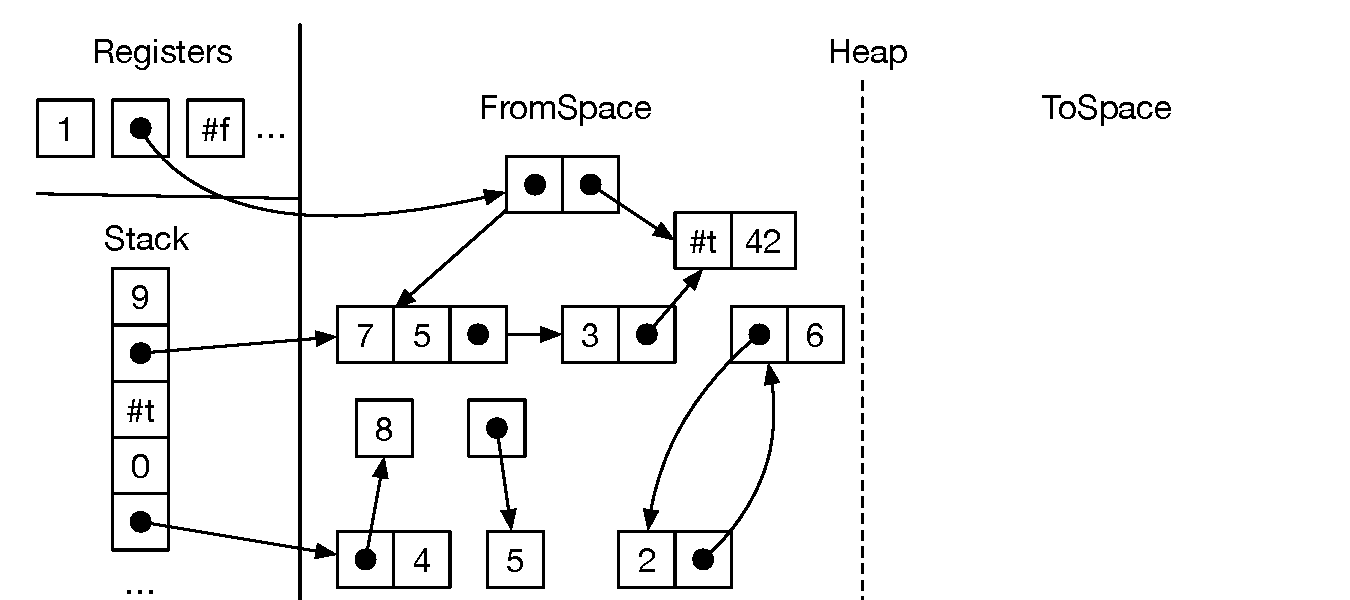
\includegraphics[width=\textwidth]{figs/copy-collect-1} \\[5ex]
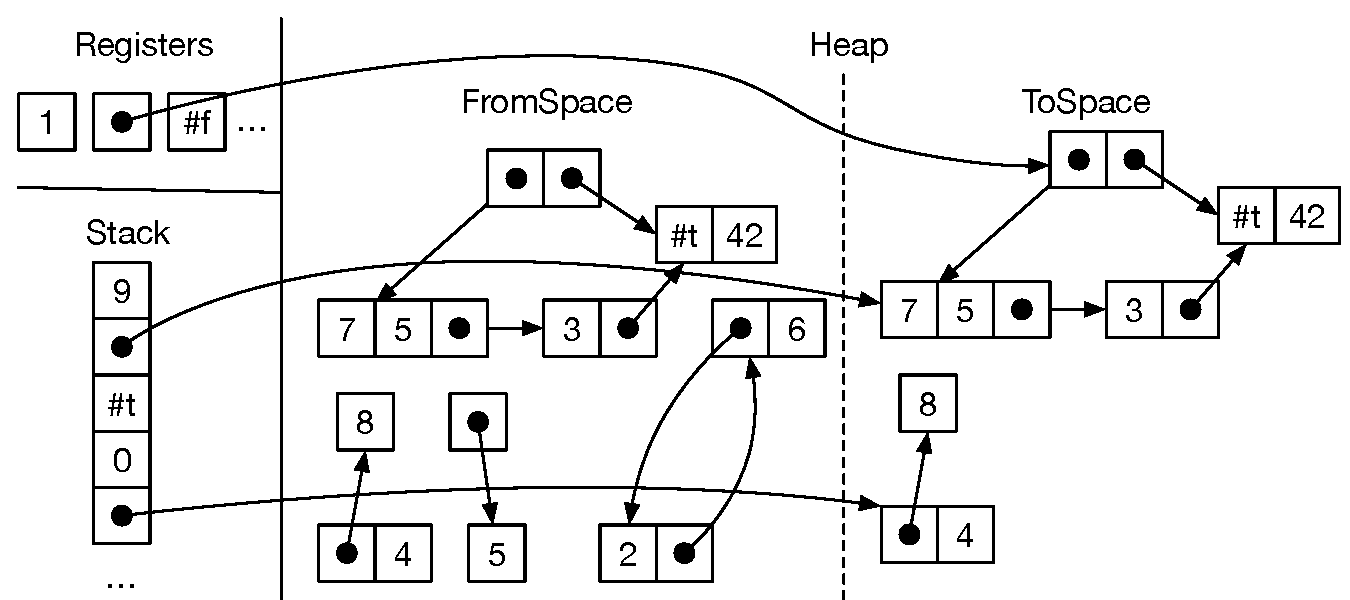
\includegraphics[width=\textwidth]{figs/copy-collect-2}
\caption{A copying collector in action.}
\label{fig:copying-collector}
\end{figure}

There are many alternatives to copying collectors (and their bigger
siblings, the generational collectors) when its comes to garbage
collection, such as mark-and-sweep~\citep{McCarthy:1960dz} and
reference counting~\citep{Collins:1960aa}.  The strengths of copying
collectors are that allocation is fast (just a comparison and pointer
increment), there is no fragmentation, cyclic garbage is collected,
and the time complexity of collection only depends on the amount of
live data, and not on the amount of garbage~\citep{Wilson:1992fk}. The
main disadvantages of a two-space copying collector is that it uses a
lot of space and takes a long time to perform the copy, though these
problems are ameliorated in generational collectors.  Racket and
Scheme programs tend to allocate many small objects and generate a lot
of garbage, so copying and generational collectors are a good fit.
Garbage collection is an active research topic, especially concurrent
garbage collection~\citep{Tene:2011kx}. Researchers are continuously
developing new techniques and revisiting old
trade-offs~\citep{Blackburn:2004aa,Jones:2011aa,Shahriyar:2013aa,Cutler:2015aa,Shidal:2015aa,Osterlund:2016aa,Jacek:2019aa,Gamari:2020aa}. Researchers
meet every year at the International Symposium on Memory Management to
present these findings.


\subsection{Graph Copying via Cheney's Algorithm}
\label{sec:cheney}
\index{Cheney's algorithm}
Let us take a closer look at the copying of the live objects. The
allocated objects and pointers can be viewed as a graph and we need to
copy the part of the graph that is reachable from the root set. To
make sure we copy all of the reachable vertices in the graph, we need
an exhaustive graph traversal algorithm, such as depth-first search or
breadth-first search~\citep{Moore:1959aa,Cormen:2001uq}. Recall that
such algorithms take into account the possibility of cycles by marking
which vertices have already been visited, so as to ensure termination
of the algorithm. These search algorithms also use a data structure
such as a stack or queue as a to-do list to keep track of the vertices
that need to be visited. We use breadth-first search and a trick
due to \citet{Cheney:1970aa} for simultaneously representing the queue
and copying tuples into the ToSpace.

Figure~\ref{fig:cheney} shows several snapshots of the ToSpace as the
copy progresses. The queue is represented by a chunk of contiguous
memory at the beginning of the ToSpace, using two pointers to track
the front and the back of the queue. The algorithm starts by copying
all tuples that are immediately reachable from the root set into the
ToSpace to form the initial queue.  When we copy a tuple, we mark the
old tuple to indicate that it has been visited. We discuss how this
marking is accomplish in Section~\ref{sec:data-rep-gc}. Note that any
pointers inside the copied tuples in the queue still point back to the
FromSpace. Once the initial queue has been created, the algorithm
enters a loop in which it repeatedly processes the tuple at the front
of the queue and pops it off the queue.  To process a tuple, the
algorithm copies all the tuple that are directly reachable from it to
the ToSpace, placing them at the back of the queue. The algorithm then
updates the pointers in the popped tuple so they point to the newly
copied tuples.

\begin{figure}[tbp]
\centering 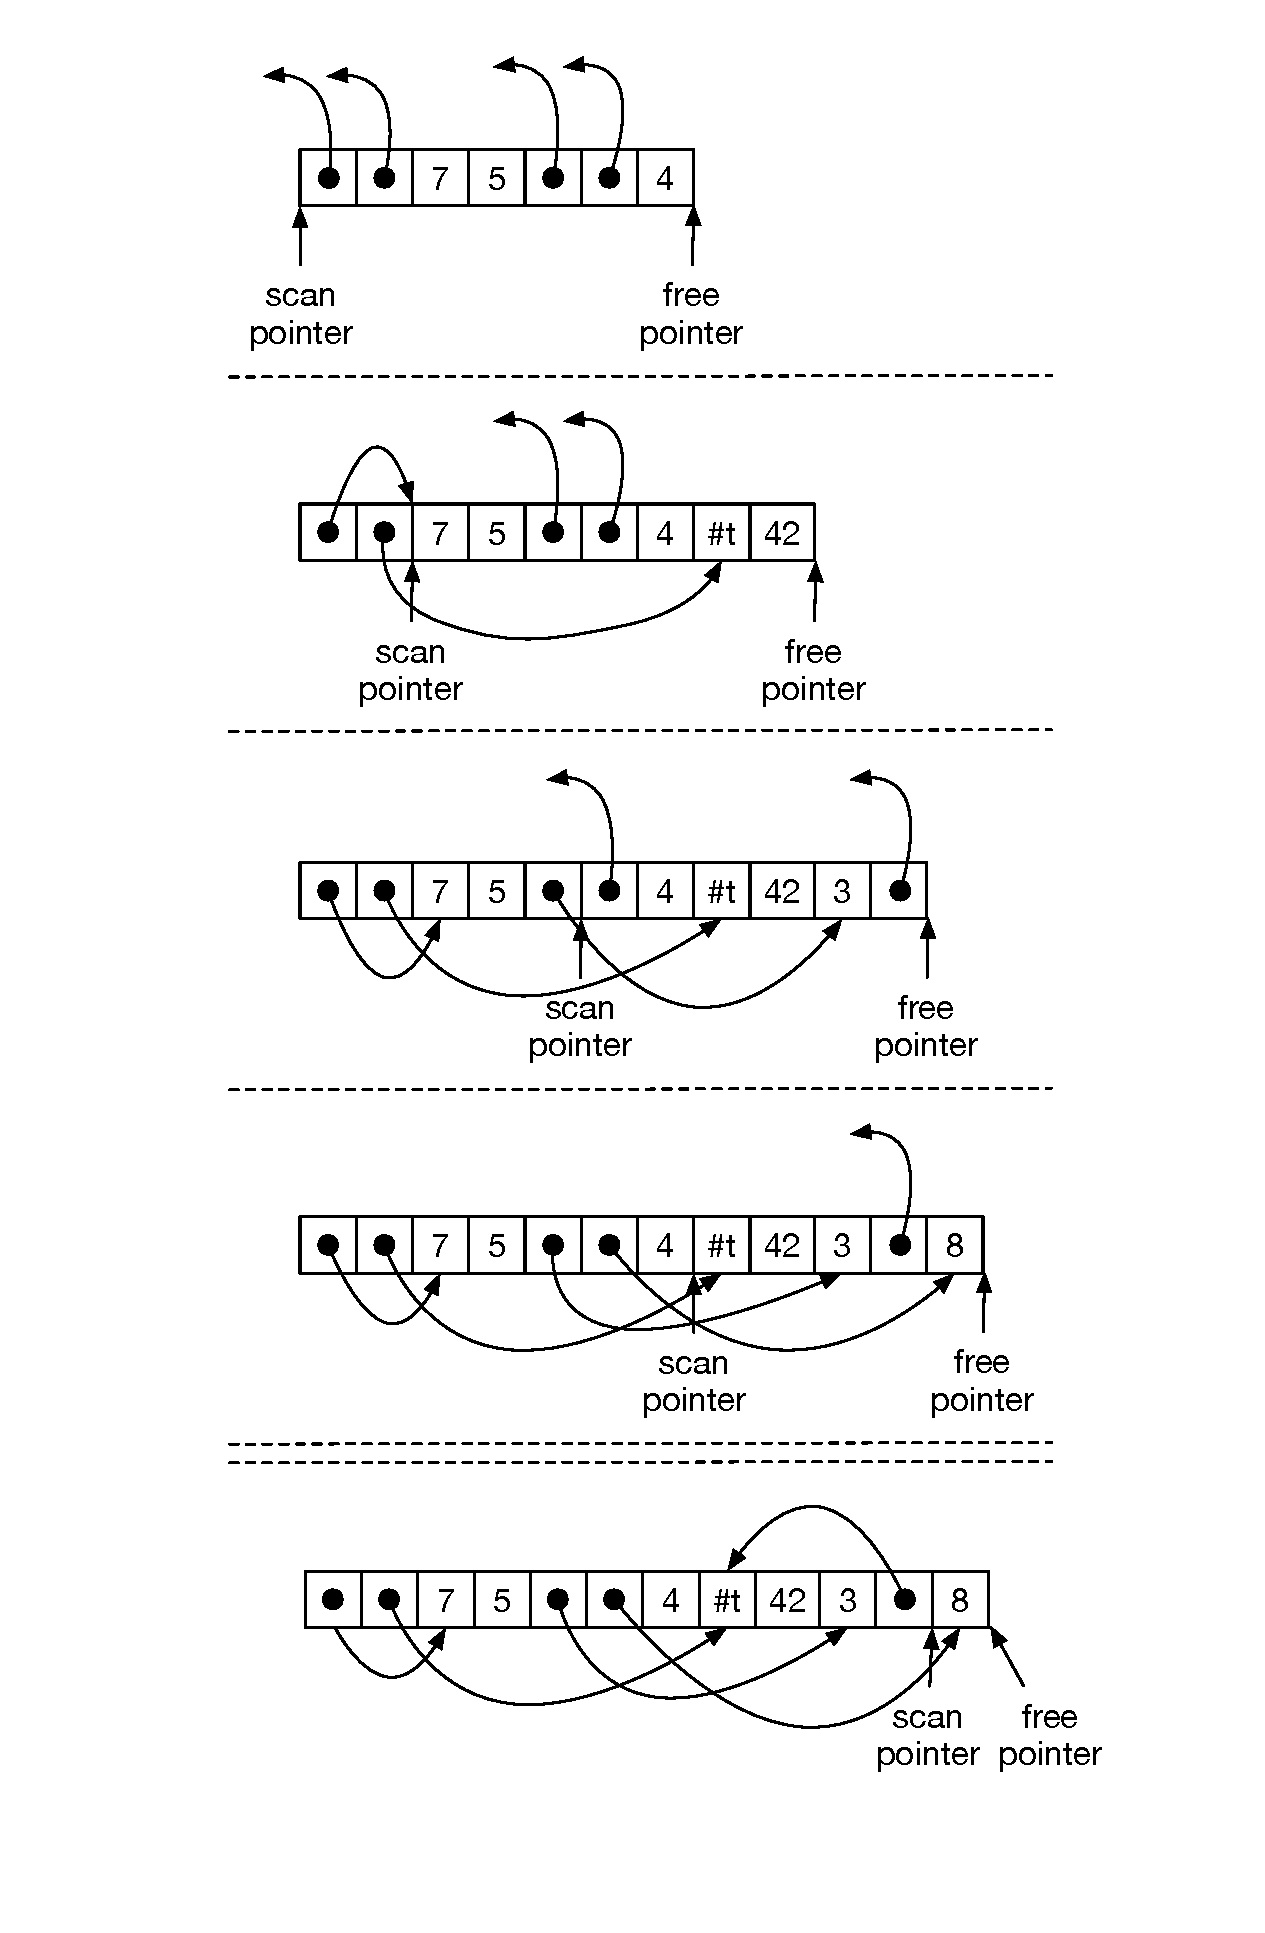
\includegraphics[width=0.9\textwidth]{figs/cheney}
\caption{Depiction of the Cheney algorithm copying the live tuples.}
\label{fig:cheney}
\end{figure}

Getting back to Figure~\ref{fig:cheney}, in the first step we copy the
tuple whose second element is $42$ to the back of the queue. The other
pointer goes to a tuple that has already been copied, so we do not
need to copy it again, but we do need to update the pointer to the new
location. This can be accomplished by storing a \emph{forwarding
pointer} to the new location in the old tuple, back when we initially
copied the tuple into the ToSpace. This completes one step of the
algorithm. The algorithm continues in this way until the front of the
queue is empty, that is, until the front catches up with the back.


\subsection{Data Representation}
\label{sec:data-rep-gc}

The garbage collector places some requirements on the data
representations used by our compiler. First, the garbage collector
needs to distinguish between pointers and other kinds of data. There
are several ways to accomplish this.
\begin{enumerate}
\item Attached a tag to each object that identifies what type of
  object it is~\citep{McCarthy:1960dz}.
\item Store different types of objects in different
  regions~\citep{Steele:1977ab}.
\item Use type information from the program to either generate
  type-specific code for collecting or to generate tables that can
  guide the
  collector~\citep{Appel:1989aa,Goldberg:1991aa,Diwan:1992aa}.
\end{enumerate}
Dynamically typed languages, such as Lisp, need to tag objects
anyways, so option 1 is a natural choice for those languages.
However, $R_3$ is a statically typed language, so it would be
unfortunate to require tags on every object, especially small and
pervasive objects like integers and Booleans.  Option 3 is the
best-performing choice for statically typed languages, but comes with
a relatively high implementation complexity. To keep this chapter
within a 2-week time budget, we recommend a combination of options 1
and 2, using separate strategies for the stack and the heap.

Regarding the stack, we recommend using a separate stack for pointers,
which we call a \emph{root stack}\index{root stack} (a.k.a. ``shadow
stack'')~\citep{Siebert:2001aa,Henderson:2002aa,Baker:2009aa}. That
is, when a local variable needs to be spilled and is of type
\code{(Vector $\Type_1 \ldots \Type_n$)}, then we put it on the root
stack instead of the normal procedure call stack. Furthermore, we
always spill vector-typed variables if they are live during a call to
the collector, thereby ensuring that no pointers are in registers
during a collection. Figure~\ref{fig:shadow-stack} reproduces the
example from Figure~\ref{fig:copying-collector} and contrasts it with
the data layout using a root stack. The root stack contains the two
pointers from the regular stack and also the pointer in the second
register.

\begin{figure}[tbp]
\centering 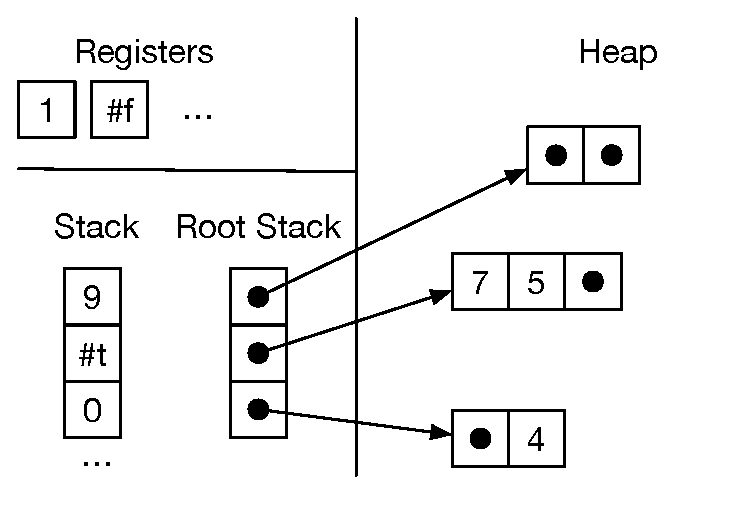
\includegraphics[width=0.60\textwidth]{figs/root-stack}
\caption{Maintaining a root stack to facilitate garbage collection.}
\label{fig:shadow-stack}
\end{figure}

The problem of distinguishing between pointers and other kinds of data
also arises inside of each tuple on the heap. We solve this problem by
attaching a tag, an extra 64-bits, to each
tuple. Figure~\ref{fig:tuple-rep} zooms in on the tags for two of the
tuples in the example from Figure~\ref{fig:copying-collector}. Note
that we have drawn the bits in a big-endian way, from right-to-left,
with bit location 0 (the least significant bit) on the far right,
which corresponds to the direction of the x86 shifting instructions
\key{salq} (shift left) and \key{sarq} (shift right). Part of each tag
is dedicated to specifying which elements of the tuple are pointers,
the part labeled ``pointer mask''. Within the pointer mask, a 1 bit
indicates there is a pointer and a 0 bit indicates some other kind of
data. The pointer mask starts at bit location 7. We have limited
tuples to a maximum size of 50 elements, so we just need 50 bits for
the pointer mask. The tag also contains two other pieces of
information. The length of the tuple (number of elements) is stored in
bits location 1 through 6. Finally, the bit at location 0 indicates
whether the tuple has yet to be copied to the ToSpace.  If the bit has
value 1, then this tuple has not yet been copied.  If the bit has
value 0 then the entire tag is a forwarding pointer. (The lower 3 bits
of a pointer are always zero anyways because our tuples are 8-byte
aligned.)

\begin{figure}[tbp]
\centering 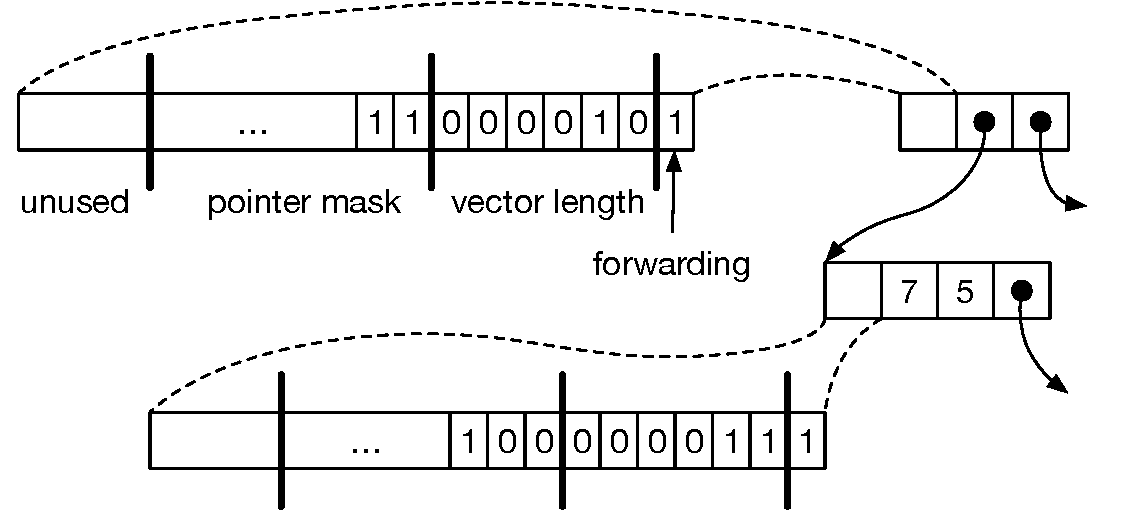
\includegraphics[width=0.8\textwidth]{figs/tuple-rep}
\caption{Representation of tuples in the heap.}
\label{fig:tuple-rep}
\end{figure}

\subsection{Implementation of the Garbage Collector}
\label{sec:organize-gz}
\index{prelude}

An implementation of the copying collector is provided in the
\code{runtime.c} file. Figure~\ref{fig:gc-header} defines the
interface to the garbage collector that is used by the compiler. The
\code{initialize} function creates the FromSpace, ToSpace, and root
stack and should be called in the prelude of the \code{main}
function. The \code{initialize} function puts the address of the
beginning of the FromSpace into the global variable
\code{free\_ptr}. The global variable \code{fromspace\_end} points to
the address that is 1-past the last element of the FromSpace. (We use
half-open intervals to represent chunks of
memory~\citep{Dijkstra:1982aa}.)  The \code{rootstack\_begin} variable
points to the first element of the root stack.

As long as there is room left in the FromSpace, your generated code
can allocate tuples simply by moving the \code{free\_ptr} forward.
%
The amount of room left in FromSpace is the difference between the
\code{fromspace\_end} and the \code{free\_ptr}.  The \code{collect}
function should be called when there is not enough room left in the
FromSpace for the next allocation.  The \code{collect} function takes
a pointer to the current top of the root stack (one past the last item
that was pushed) and the number of bytes that need to be
allocated. The \code{collect} function performs the copying collection
and leaves the heap in a state such that the next allocation will
succeed.

\begin{figure}[tbp]
\begin{lstlisting}
   void initialize(uint64_t rootstack_size, uint64_t heap_size);
   void collect(int64_t** rootstack_ptr, uint64_t bytes_requested);
   int64_t* free_ptr;
   int64_t* fromspace_begin;
   int64_t* fromspace_end;
   int64_t** rootstack_begin;
\end{lstlisting}
\caption{The compiler's interface to the garbage collector.}
\label{fig:gc-header}
\end{figure}

%% \begin{exercise}
%%   In the file \code{runtime.c} you will find the implementation of
%%   \code{initialize} and a partial implementation of \code{collect}.
%%   The \code{collect} function calls another function, \code{cheney},
%%   to perform the actual copy, and that function is left to the reader
%%   to implement. The following is the prototype for \code{cheney}.
%% \begin{lstlisting}
%%    static void cheney(int64_t** rootstack_ptr);
%% \end{lstlisting}
%%   The parameter \code{rootstack\_ptr} is a pointer to the top of the
%%   rootstack (which is an array of pointers).  The \code{cheney} function
%%   also communicates with \code{collect} through the global
%%   variables \code{fromspace\_begin} and \code{fromspace\_end}
%%   mentioned in Figure~\ref{fig:gc-header} as well as the pointers for
%%   the ToSpace:
%% \begin{lstlisting}
%%    static int64_t* tospace_begin;
%%    static int64_t* tospace_end;
%% \end{lstlisting}
%%   The job of the \code{cheney} function is to copy all the live
%%   objects (reachable from the root stack) into the ToSpace, update
%%   \code{free\_ptr} to point to the next unused spot in the ToSpace,
%%   update the root stack so that it points to the objects in the
%%   ToSpace, and finally to swap the global pointers for the FromSpace
%%   and ToSpace.
%% \end{exercise}


%% \section{Compiler Passes}
%% \label{sec:code-generation-gc}

The introduction of garbage collection has a non-trivial impact on our
compiler passes. We introduce two new compiler passes named
\code{expose-allocation} and \code{uncover-locals}. We make
significant changes to \code{select-instructions},
\code{build-interference}, \code{allocate-registers}, and
\code{print-x86} and make minor changes in severl more passes.  The
following program will serve as our running example.  It creates two
tuples, one nested inside the other. Both tuples have length one. The
program accesses the element in the inner tuple tuple via two vector
references.
% tests/s2_17.rkt
\begin{lstlisting}
(vector-ref (vector-ref (vector (vector 42)) 0) 0))
\end{lstlisting}

\section{Shrink}
\label{sec:shrink-R3}

Recall that the \code{shrink} pass translates the primitives operators
into a smaller set of primitives. Because this pass comes after type
checking, but before the passes that require the type information in
the \code{HasType} AST nodes, the \code{shrink} pass must be modified
to wrap \code{HasType} around each AST node that it generates.


\section{Expose Allocation}
\label{sec:expose-allocation}

The pass \code{expose-allocation} lowers the \code{vector} creation
form into a conditional call to the collector followed by the
allocation.  We choose to place the \code{expose-allocation} pass
before \code{remove-complex-opera*} because the code generated by
\code{expose-allocation} contains complex operands.  We also place
\code{expose-allocation} before \code{explicate-control} because
\code{expose-allocation} introduces new variables using \code{let},
but \code{let} is gone after \code{explicate-control}.

The output of \code{expose-allocation} is a language $R'_3$ that
extends $R_3$ with the three new forms that we use in the translation
of the \code{vector} form.
\[
\begin{array}{lcl}
  \Exp &::=& \cdots
      \mid (\key{collect} \,\itm{int})
      \mid (\key{allocate} \,\itm{int}\,\itm{type})
      \mid (\key{global-value} \,\itm{name})
\end{array}
\]
The $(\key{collect}\,n)$ form runs the garbage collector, requesting
$n$ bytes. It will become a call to the \code{collect} function in
\code{runtime.c} in \code{select-instructions}.  The
$(\key{allocate}\,n\,T)$ form creates an tuple of $n$ elements.
\index{allocate}
The $T$ parameter is the type of the tuple: \code{(Vector $\Type_1 \ldots
  \Type_n$)} where $\Type_i$ is the type of the $i$th element in the
tuple. The $(\key{global-value}\,\itm{name})$ form reads the value of
a global variable, such as \code{free\_ptr}.

In the following, we show the transformation for the \code{vector}
form into 1) a sequence of let-bindings for the initializing
expressions, 2) a conditional call to \code{collect}, 3) a call to
\code{allocate}, and 4) the initialization of the vector. In the
following, \itm{len} refers to the length of the vector and
\itm{bytes} is how many total bytes need to be allocated for the
vector, which is 8 for the tag plus \itm{len} times 8.
\begin{lstlisting}
  (has-type (vector |$e_0 \ldots e_{n-1}$|) |\itm{type}|)
|$\Longrightarrow$|
  (let ([|$x_0$| |$e_0$|]) ... (let ([|$x_{n-1}$| |$e_{n-1}$|])
  (let ([_ (if (< (+ (global-value free_ptr) |\itm{bytes}|)
                  (global-value fromspace_end))
               (void)
               (collect |\itm{bytes}|))])
  (let ([|$v$| (allocate |\itm{len}| |\itm{type}|)])
  (let ([_ (vector-set! |$v$| |$0$| |$x_0$|)]) ...
  (let ([_ (vector-set! |$v$| |$n-1$| |$x_{n-1}$|)])
     |$v$|) ... )))) ...)
\end{lstlisting}
In the above, we suppressed all of the \code{has-type} forms in the
output for the sake of readability.  The placement of the initializing
expressions $e_0,\ldots,e_{n-1}$ prior to the \code{allocate} and the
sequence of \code{vector-set!} is important, as those expressions may
trigger garbage collection and we cannot have an allocated but
uninitialized tuple on the heap during a collection.

Figure~\ref{fig:expose-alloc-output} shows the output of the
\code{expose-allocation} pass on our running example.

\begin{figure}[tbp]
% tests/s2_17.rkt
\begin{lstlisting}
(vector-ref
 (vector-ref
  (let ([vecinit7976
         (let ([vecinit7972 42])
           (let ([collectret7974
                  (if (< (+ (global-value free_ptr) 16) 
                         (global-value fromspace_end))
                      (void)
                      (collect 16)
                      )])
             (let ([alloc7971 (allocate 1 (Vector Integer))])
               (let ([initret7973 (vector-set! alloc7971 0 vecinit7972)])
                 alloc7971)
               )
             )
           )
         ])
    (let ([collectret7978
           (if (< (+ (global-value free_ptr) 16)
                  (global-value fromspace_end))
               (void)
               (collect 16)
               )])
      (let ([alloc7975 (allocate 1 (Vector (Vector Integer)))])
        (let ([initret7977 (vector-set! alloc7975 0 vecinit7976)])
          alloc7975)
        )
      )
    )
  0)
 0)
\end{lstlisting}
\caption{Output of the \code{expose-allocation} pass, minus
  all of the \code{has-type} forms.}
\label{fig:expose-alloc-output}
\end{figure}


\section{Remove Complex Operands}
\label{sec:remove-complex-opera-R3}

The new forms \code{collect}, \code{allocate}, and \code{global-value}
should all be treated as complex operands. A new case for
\code{HasType} is needed and the case for \code{Prim} needs to be
handled carefully to prevent the \code{Prim} node from being separated
from its enclosing \code{HasType}.


\section{Explicate Control and the $C_2$ language}
\label{sec:explicate-control-r3}

\begin{figure}[tbp]
\fbox{
\begin{minipage}{0.96\textwidth}
\small    
\[
\begin{array}{lcl}
\Atm &::=& \gray{ \Int \mid \Var \mid \itm{bool} } \\
\itm{cmp} &::= & \gray{ \key{eq?} \mid \key{<} } \\
\Exp &::=& \gray{ \Atm \mid \key{(read)} \mid \key{(-}~\Atm\key{)} \mid \key{(+}~\Atm~\Atm\key{)} } \\
  &\mid& \gray{ \LP \key{not}~\Atm \RP \mid \LP \itm{cmp}~\Atm~\Atm\RP } \\
&\mid& \LP \key{allocate}~\Int~\Type \RP \\
  &\mid& (\key{vector-ref}\;\Atm\;\Int) \mid (\key{vector-set!}\;\Atm\;\Int\;\Atm)\\
  &\mid& \LP \key{global-value}~\Var \RP \mid \LP \key{void} \RP \\
\Stmt &::=& \gray{ \Var~\key{=}~\Exp\key{;} } \mid \LP\key{collect}~\Int \RP\\
\Tail &::= & \gray{ \key{return}~\Exp\key{;} \mid \Stmt~\Tail } 
   \mid \gray{ \key{goto}~\itm{label}\key{;} }\\
   &\mid& \gray{ \key{if}~\LP \itm{cmp}~\Atm~\Atm \RP~ \key{goto}~\itm{label}\key{;} ~\key{else}~\key{goto}~\itm{label}\key{;} } \\
C_2 & ::= & \gray{ (\itm{label}\key{:}~ \Tail)\ldots }
\end{array}
\]
\end{minipage}
}
\caption{The concrete syntax of the $C_2$ intermediate language.}
\label{fig:c2-concrete-syntax}
\end{figure}

\begin{figure}[tp]
\fbox{
  \begin{minipage}{0.96\textwidth}
    \small
\[
\begin{array}{lcl}
\Atm &::=& \gray{ \INT{\Int} \mid \VAR{\Var} \mid \BOOL{\itm{bool}} }\\
\itm{cmp} &::= & \gray{  \key{eq?} \mid \key{<} } \\
\Exp &::= & \gray{ \Atm \mid \READ{} } \\
   &\mid& \gray{ \NEG{\Atm} \mid \ADD{\Atm}{\Atm} }\\
   &\mid& \gray{ \UNIOP{\key{not}}{\Atm} \mid \BINOP{\itm{cmp}}{\Atm}{\Atm}  } \\
   &\mid& (\key{Allocate} \,\itm{int}\,\itm{type}) \\
   &\mid& \BINOP{\key{'vector-ref}}{\Atm}{\INT{\Int}}  \\
   &\mid& (\key{Prim}~\key{'vector-set!}\,(\key{list}\,\Atm\,\INT{\Int}\,\Atm))\\
   &\mid& (\key{GlobalValue} \,\Var) \mid (\key{Void})\\
\Stmt &::=& \gray{ \ASSIGN{\VAR{\Var}}{\Exp} } 
       \mid (\key{Collect} \,\itm{int}) \\
\Tail &::= & \gray{ \RETURN{\Exp} \mid \SEQ{\Stmt}{\Tail} 
       \mid \GOTO{\itm{label}} } \\
      &\mid& \gray{ \IFSTMT{\BINOP{\itm{cmp}}{\Atm}{\Atm}}{\GOTO{\itm{label}}}{\GOTO{\itm{label}}}  }\\
C_2 & ::= & \gray{ \PROGRAM{\itm{info}}{\CFG{(\itm{label}\,\key{.}\,\Tail)\ldots}} }
\end{array}
\]
\end{minipage}
}
\caption{The abstract syntax of $C_2$, extending $C_1$
   (Figure~\ref{fig:c1-syntax}).}
\label{fig:c2-syntax}
\end{figure}

The output of \code{explicate-control} is a program in the
intermediate language $C_2$, whose concrete syntax is defined in
Figure~\ref{fig:c2-concrete-syntax} and whose abstract syntax is
defined in Figure~\ref{fig:c2-syntax}.  The new forms of $C_2$ include
the \key{allocate}, \key{vector-ref}, and \key{vector-set!}, and
\key{global-value} expressions and the \code{collect} statement.  The
\code{explicate-control} pass can treat these new forms much like the
other forms.


\section{Uncover Locals}
\label{sec:uncover-locals-r3}

Recall that the \code{explicate-control} function collects all of the
local variables so that it can store them in the $\itm{info}$ field of
the \code{Program} structure. Also recall that we need to know the
types of all the local variables for purposes of identifying the root
set for the garbage collector.  Thus, we create a pass named
\code{uncover-locals} to collect not just the variables but the
variables and their types in the form of an alist. Thanks to the
\code{HasType} nodes, the types are readily available at every
assignment to a variable. We recommend storing the resulting alist in
the $\itm{info}$ field of the program, associated with the
\code{locals} key. Figure~\ref{fig:uncover-locals-r3} lists the output
of the \code{uncover-locals} pass on the running example.

\begin{figure}[tbp]
% tests/s2_17.rkt
\begin{lstlisting}
locals:
    vecinit7976 : '(Vector Integer), tmp7980 : 'Integer,
    alloc7975 : '(Vector (Vector Integer)), tmp7983 : 'Integer,
    collectret7974 : 'Void, initret7977 : 'Void,
    collectret7978 : 'Void, tmp7985 : '(Vector Integer),
    tmp7984 : 'Integer, tmp7979 : 'Integer, tmp7982 : 'Integer,
    alloc7971 : '(Vector Integer), tmp7981 : 'Integer,
    vecinit7972 : 'Integer, initret7973 : 'Void, 
block91:
    (collect 16)
    goto block89;
block90:
    collectret7974 = (void);
    goto block89;
block89:
    alloc7971 = (allocate 1 (Vector Integer));
    initret7973 = (vector-set! alloc7971 0 vecinit7972);
    vecinit7976 = alloc7971;
    tmp7982 = (global-value free_ptr);
    tmp7983 = (+ tmp7982 16);
    tmp7984 = (global-value fromspace_end);
    if (< tmp7983 tmp7984) then
       goto block87;
    else
       goto block88;
block88:
    (collect 16)
    goto block86;
block87:
    collectret7978 = (void);
    goto block86;
block86:
    alloc7975 = (allocate 1 (Vector (Vector Integer)));
    initret7977 = (vector-set! alloc7975 0 vecinit7976);
    tmp7985 = (vector-ref alloc7975 0);
    return (vector-ref tmp7985 0);
start:
    vecinit7972 = 42;
    tmp7979 = (global-value free_ptr);
    tmp7980 = (+ tmp7979 16);
    tmp7981 = (global-value fromspace_end);
    if (< tmp7980 tmp7981) then
       goto block90;
    else
       goto block91;
\end{lstlisting}
\caption{Output of \code{uncover-locals} for the running example.}
\label{fig:uncover-locals-r3}
\end{figure}

\clearpage

\section{Select Instructions and the x86$_2$ Language}
\label{sec:select-instructions-gc}
\index{instruction selection}

%% void (rep as zero)
%% allocate
%% collect (callq collect)
%% vector-ref
%% vector-set!
%% global (postpone)

In this pass we generate x86 code for most of the new operations that
were needed to compile tuples, including \code{Allocate},
\code{Collect}, \code{vector-ref}, \code{vector-set!}, and
\code{void}. We compile \code{GlobalValue} to \code{Global} because
the later has a different concrete syntax (see
Figures~\ref{fig:x86-2-concrete} and \ref{fig:x86-2}).
\index{x86}

The \code{vector-ref} and \code{vector-set!} forms translate into
\code{movq} instructions.  (The plus one in the offset is to get past
the tag at the beginning of the tuple representation.)
\begin{lstlisting}
|$\itm{lhs}$| = (vector-ref |$\itm{vec}$| |$n$|);
|$\Longrightarrow$|
movq |$\itm{vec}'$|, %r11
movq |$8(n+1)$|(%r11), |$\itm{lhs'}$|

|$\itm{lhs}$| = (vector-set! |$\itm{vec}$| |$n$| |$\itm{arg}$|);
|$\Longrightarrow$|
movq |$\itm{vec}'$|, %r11
movq |$\itm{arg}'$|, |$8(n+1)$|(%r11)
movq $0, |$\itm{lhs'}$|
\end{lstlisting}
The $\itm{lhs}'$, $\itm{vec}'$, and $\itm{arg}'$ are obtained by
translating $\itm{vec}$ and $\itm{arg}$ to x86.  The move of $\itm{vec}'$ to
register \code{r11} ensures that offset expression
\code{$-8(n+1)$(\%r11)} contains a register operand.  This requires
removing \code{r11} from consideration by the register allocating.

Why not use \code{rax} instead of \code{r11}? Suppose we instead used
\code{rax}. Then the generated code for \code{vector-set!} would be
\begin{lstlisting}
movq |$\itm{vec}'$|, %rax
movq |$\itm{arg}'$|, |$8(n+1)$|(%rax)
movq $0, |$\itm{lhs}'$|
\end{lstlisting}
Next, suppose that $\itm{arg}'$ ends up as a stack location, so
\code{patch-instructions} would insert a move through \code{rax}
as follows.
\begin{lstlisting}
movq |$\itm{vec}'$|, %rax
movq |$\itm{arg}'$|, %rax
movq %rax, |$8(n+1)$|(%rax)
movq $0, |$\itm{lhs}'$|
\end{lstlisting}
But the above sequence of instructions does not work because we're
trying to use \code{rax} for two different values ($\itm{vec}'$ and
$\itm{arg}'$) at the same time!

We compile the \code{allocate} form to operations on the
\code{free\_ptr}, as shown below. The address in the \code{free\_ptr}
is the next free address in the FromSpace, so we copy it into
\code{r11} and then move it forward by enough space for the tuple
being allocated, which is $8(\itm{len}+1)$ bytes because each element
is 8 bytes (64 bits) and we use 8 bytes for the tag.  We then
initialize the \itm{tag} and finally copy the address in \code{r11} to
the left-hand-side. Refer to Figure~\ref{fig:tuple-rep} to see how the
tag is organized. We recommend using the Racket operations
\code{bitwise-ior} and \code{arithmetic-shift} to compute the tag
during compilation.  The type annotation in the \code{vector} form is
used to determine the pointer mask region of the tag.
\begin{lstlisting}
   |$\itm{lhs}$| = (allocate |$\itm{len}$| (Vector |$\itm{type} \ldots$|));
   |$\Longrightarrow$|
   movq free_ptr(%rip), %r11
   addq |$8(\itm{len}+1)$|, free_ptr(%rip)
   movq $|$\itm{tag}$|, 0(%r11)
   movq %r11, |$\itm{lhs}'$|
\end{lstlisting}

The \code{collect} form is compiled to a call to the \code{collect}
function in the runtime. The arguments to \code{collect} are 1) the
top of the root stack and 2) the number of bytes that need to be
allocated.  We use another dedicated register, \code{r15}, to
store the pointer to the top of the root stack. So \code{r15} is not
available for use by the register allocator.
\begin{lstlisting}
   (collect |$\itm{bytes}$|)
   |$\Longrightarrow$|
   movq %r15, %rdi
   movq $|\itm{bytes}|, %rsi
   callq collect
\end{lstlisting}



\begin{figure}[tp]
\fbox{
\begin{minipage}{0.96\textwidth}
\[
\begin{array}{lcl}
  \Arg &::=& \gray{ \key{\$}\Int \mid \key{\%}\Reg \mid \Int\key{(}\key{\%}\Reg\key{)} \mid \key{\%}\itm{bytereg} } \mid \Var \key{(\%rip)} \\
x86_1 &::= & \gray{ \key{.globl main} }\\
      &    & \gray{ \key{main:} \; \Instr\ldots }
\end{array}
\]
\end{minipage}
}
\caption{The concrete syntax of x86$_2$  (extends x86$_1$ of Figure~\ref{fig:x86-1-concrete}).}
\label{fig:x86-2-concrete}
\end{figure}

\begin{figure}[tp]
\fbox{
  \begin{minipage}{0.96\textwidth}
    \small
\[
\begin{array}{lcl}
  \Arg &::=&  \gray{  \INT{\Int} \mid \REG{\Reg} \mid \DEREF{\Reg}{\Int}
   \mid \BYTEREG{\Reg}} \\
   &\mid& (\key{Global}~\Var) \\
x86_2 &::= & \gray{ \PROGRAM{\itm{info}}{\CFG{\key{(}\itm{label} \,\key{.}\, \Block \key{)}\ldots}} }
\end{array}
\]
\end{minipage}
}
\caption{The abstract syntax of x86$_2$ (extends x86$_1$ of Figure~\ref{fig:x86-1}).}
\label{fig:x86-2}
\end{figure}

The concrete and abstract syntax of the $x86_2$ language is defined in
Figures~\ref{fig:x86-2-concrete} and \ref{fig:x86-2}.  It differs from
x86$_1$ just in the addition of the form for global variables.
%
Figure~\ref{fig:select-instr-output-gc} shows the output of the
\code{select-instructions} pass on the running example.

\begin{figure}[tbp]
\centering
% tests/s2_17.rkt
\begin{minipage}[t]{0.5\textwidth}
\begin{lstlisting}[basicstyle=\ttfamily\scriptsize]
block35:
    movq free_ptr(%rip), alloc9024
    addq $16, free_ptr(%rip)
    movq alloc9024, %r11
    movq $131, 0(%r11)
    movq alloc9024, %r11
    movq vecinit9025, 8(%r11)
    movq $0, initret9026
    movq alloc9024, %r11
    movq 8(%r11), tmp9034
    movq tmp9034, %r11
    movq 8(%r11), %rax
    jmp conclusion
block36:
    movq $0, collectret9027
    jmp block35
block38:
    movq free_ptr(%rip), alloc9020
    addq $16, free_ptr(%rip)
    movq alloc9020, %r11
    movq $3, 0(%r11)
    movq alloc9020, %r11
    movq vecinit9021, 8(%r11)
    movq $0, initret9022
    movq alloc9020, vecinit9025
    movq free_ptr(%rip), tmp9031
    movq tmp9031, tmp9032
    addq $16, tmp9032
    movq fromspace_end(%rip), tmp9033
    cmpq tmp9033, tmp9032
    jl block36
    jmp block37
block37:
    movq %r15, %rdi
    movq $16, %rsi
    callq 'collect
    jmp block35
block39:
    movq $0, collectret9023
    jmp block38
\end{lstlisting}
\end{minipage}
\begin{minipage}[t]{0.45\textwidth}
\begin{lstlisting}[basicstyle=\ttfamily\scriptsize]
start:
    movq $42, vecinit9021
    movq free_ptr(%rip), tmp9028
    movq tmp9028, tmp9029
    addq $16, tmp9029
    movq fromspace_end(%rip), tmp9030
    cmpq tmp9030, tmp9029
    jl block39
    jmp block40
block40:
    movq %r15, %rdi
    movq $16, %rsi
    callq 'collect
    jmp block38
\end{lstlisting}
\end{minipage}
\caption{Output of the \code{select-instructions} pass.}
\label{fig:select-instr-output-gc}
\end{figure}

\clearpage

\section{Register Allocation}
\label{sec:reg-alloc-gc}
\index{register allocation}

As discussed earlier in this chapter, the garbage collector needs to
access all the pointers in the root set, that is, all variables that
are vectors. It will be the responsibility of the register allocator
to make sure that:
\begin{enumerate}
\item the root stack is used for spilling vector-typed variables, and
\item if a vector-typed variable is live during a call to the
  collector, it must be spilled to ensure it is visible to the
  collector.
\end{enumerate}

The later responsibility can be handled during construction of the
inference graph, by adding interference edges between the call-live
vector-typed variables and all the callee-saved registers. (They
already interfere with the caller-saved registers.)  The type
information for variables is in the \code{Program} form, so we
recommend adding another parameter to the \code{build-interference}
function to communicate this alist.

The spilling of vector-typed variables to the root stack can be
handled after graph coloring, when choosing how to assign the colors
(integers) to registers and stack locations. The \code{Program} output
of this pass changes to also record the number of spills to the root
stack.

% build-interference
%
% callq
%   extra parameter for var->type assoc. list
% update 'program' and 'if'

% allocate-registers
%    allocate spilled vectors to the rootstack

% don't change color-graph



\section{Print x86}
\label{sec:print-x86-gc}
\index{prelude}\index{conclusion}

Figure~\ref{fig:print-x86-output-gc} shows the output of the
\code{print-x86} pass on the running example. In the prelude and
conclusion of the \code{main} function, we treat the root stack very
much like the regular stack in that we move the root stack pointer
(\code{r15}) to make room for the spills to the root stack, except
that the root stack grows up instead of down.  For the running
example, there was just one spill so we increment \code{r15} by 8
bytes. In the conclusion we decrement \code{r15} by 8 bytes.

One issue that deserves special care is that there may be a call to
\code{collect} prior to the initializing assignments for all the
variables in the root stack. We do not want the garbage collector to
accidentally think that some uninitialized variable is a pointer that
needs to be followed. Thus, we zero-out all locations on the root
stack in the prelude of \code{main}. In
Figure~\ref{fig:print-x86-output-gc}, the instruction
%
\lstinline{movq $0, (%r15)}
%
accomplishes this task. The garbage collector tests each root to see
if it is null prior to dereferencing it.

\begin{figure}[htbp]
\begin{minipage}[t]{0.5\textwidth}
\begin{lstlisting}[basicstyle=\ttfamily\scriptsize]
block35:
	movq	free_ptr(%rip), %rcx
	addq	$16, free_ptr(%rip)
	movq	%rcx, %r11
	movq	$131, 0(%r11)
	movq	%rcx, %r11
	movq	-8(%r15), %rax
	movq	%rax, 8(%r11)
	movq	$0, %rdx
	movq	%rcx, %r11
	movq	8(%r11), %rcx
	movq	%rcx, %r11
	movq	8(%r11), %rax
	jmp conclusion
block36:
	movq	$0, %rcx
	jmp block35
block38:
	movq	free_ptr(%rip), %rcx
	addq	$16, free_ptr(%rip)
	movq	%rcx, %r11
	movq	$3, 0(%r11)
	movq	%rcx, %r11
	movq	%rbx, 8(%r11)
	movq	$0, %rdx
	movq	%rcx, -8(%r15)
	movq	free_ptr(%rip), %rcx
	addq	$16, %rcx
	movq	fromspace_end(%rip), %rdx
	cmpq	%rdx, %rcx
	jl block36
	movq	%r15, %rdi
	movq	$16, %rsi
	callq	collect
	jmp block35
block39:
	movq	$0, %rcx
	jmp block38
\end{lstlisting}
\end{minipage}
\begin{minipage}[t]{0.45\textwidth}
\begin{lstlisting}[basicstyle=\ttfamily\scriptsize]
start:
	movq	$42, %rbx
	movq	free_ptr(%rip), %rdx
	addq	$16, %rdx
	movq	fromspace_end(%rip), %rcx
	cmpq	%rcx, %rdx
	jl block39
	movq	%r15, %rdi
	movq	$16, %rsi
	callq	collect
	jmp block38
        
	.globl main
main:
	pushq	%rbp
	movq	%rsp, %rbp
	pushq	%r13
	pushq	%r12
	pushq	%rbx
	pushq	%r14
	subq	$0, %rsp
	movq $16384, %rdi
	movq $16, %rsi
	callq initialize
	movq rootstack_begin(%rip), %r15
	movq $0, (%r15)
	addq $8, %r15
	jmp start
conclusion:
	subq $8, %r15
	addq	$0, %rsp
	popq	%r14
	popq	%rbx
	popq	%r12
	popq	%r13
	popq	%rbp
	retq
\end{lstlisting}
\end{minipage}
\caption{Output of the \code{print-x86} pass.}
\label{fig:print-x86-output-gc}
\end{figure}


\begin{figure}[p]
\begin{tikzpicture}[baseline=(current  bounding  box.center)]
\node (R3) at (0,2)  {\large $R_3$};
\node (R3-2) at (3,2)  {\large $R_3$};
\node (R3-3) at (6,2)  {\large $R_3$};
\node (R3-4) at (9,2)  {\large $R_3$};
\node (R3-5) at (9,0)  {\large $R'_3$};
\node (R3-6) at (6,0)  {\large $R'_3$};
\node (C2-4) at (3,-2)  {\large $C_2$};
\node (C2-3) at (0,-2)  {\large $C_2$};

\node (x86-2) at (3,-4)  {\large $\text{x86}^{*}_2$};
\node (x86-3) at (6,-4)  {\large $\text{x86}^{*}_2$};
\node (x86-4) at (9,-4) {\large $\text{x86}^{*}_2$};
\node (x86-5) at (9,-6) {\large $\text{x86}^{\dagger}_2$};

\node (x86-2-1) at (3,-6)  {\large $\text{x86}^{*}_2$};
\node (x86-2-2) at (6,-6)  {\large $\text{x86}^{*}_2$};

\path[->,bend left=15] (R3) edge [above] node {\ttfamily\footnotesize\color{red} type-check} (R3-2);
\path[->,bend left=15] (R3-2) edge [above] node {\ttfamily\footnotesize shrink} (R3-3);
\path[->,bend left=15] (R3-3) edge [above] node {\ttfamily\footnotesize uniquify} (R3-4);
\path[->,bend left=15] (R3-4) edge [right] node {\ttfamily\footnotesize\color{red} expose-alloc.} (R3-5);
\path[->,bend left=15] (R3-5) edge [below] node {\ttfamily\footnotesize remove-complex.} (R3-6);
\path[->,bend right=20] (R3-6) edge [left] node {\ttfamily\footnotesize explicate-control} (C2-3);
\path[->,bend right=15] (C2-3) edge [below] node {\ttfamily\footnotesize\color{red} uncover-locals} (C2-4);
\path[->,bend left=15] (C2-4) edge [right] node {\ttfamily\footnotesize\color{red} select-instr.} (x86-2);
\path[->,bend right=15] (x86-2) edge [left] node {\ttfamily\footnotesize uncover-live} (x86-2-1);
\path[->,bend right=15] (x86-2-1) edge [below] node {\ttfamily\footnotesize\color{red} build-inter.} (x86-2-2);
\path[->,bend right=15] (x86-2-2) edge [right] node {\ttfamily\footnotesize\color{red} allocate-reg.} (x86-3);
\path[->,bend left=15] (x86-3) edge [above] node {\ttfamily\footnotesize patch-instr.} (x86-4);
\path[->,bend left=15] (x86-4) edge [right] node {\ttfamily\footnotesize\color{red} print-x86} (x86-5);
\end{tikzpicture}
\caption{Diagram of the passes for $R_3$, a language with tuples.}
\label{fig:R3-passes}
\end{figure}

Figure~\ref{fig:R3-passes} gives an overview of all the passes needed
for the compilation of $R_3$.

\section{Challenge: Simple Structures}
\label{sec:simple-structures}
\index{struct}
\index{structure}

Figure~\ref{fig:r3s-concrete-syntax} defines the concrete syntax for
$R^s_3$, which extends $R^3$ with support for simple structures.
Recall that a \code{struct} in Typed Racket is a user-defined data
type that contains named fields and that is heap allocated, similar to
a vector. The following is an example of a structure definition, in
this case the definition of a \code{point} type.
\begin{lstlisting}
(struct point ([x : Integer] [y : Integer]) #:mutable)
\end{lstlisting}

\begin{figure}[tbp]
\centering
\fbox{
\begin{minipage}{0.96\textwidth}
\[
\begin{array}{lcl}
  \Type &::=& \gray{\key{Integer} \mid \key{Boolean}
  \mid (\key{Vector}\;\Type \ldots) \mid \key{Void} } \mid \Var \\
  \itm{cmp} &::= & \gray{ \key{eq?} \mid \key{<} \mid \key{<=} \mid \key{>} \mid \key{>=} } \\
  \Exp &::=& \gray{  \Int \mid (\key{read}) \mid (\key{-}\;\Exp) \mid (\key{+} \; \Exp\;\Exp) \mid (\key{-}\;\Exp\;\Exp) }  \\
  &\mid&  \gray{  \Var \mid (\key{let}~([\Var~\Exp])~\Exp)  }\\
  &\mid& \gray{ \key{\#t} \mid \key{\#f} 
   \mid (\key{and}\;\Exp\;\Exp) 
   \mid (\key{or}\;\Exp\;\Exp)
   \mid (\key{not}\;\Exp) } \\
  &\mid& \gray{  (\itm{cmp}\;\Exp\;\Exp) 
   \mid (\key{if}~\Exp~\Exp~\Exp)  } \\
  &\mid& \gray{ (\key{vector}\;\Exp \ldots) 
   \mid (\key{vector-ref}\;\Exp\;\Int) } \\
  &\mid& \gray{ (\key{vector-set!}\;\Exp\;\Int\;\Exp) }\\
  &\mid& \gray{ (\key{void}) } \mid (\Var\;\Exp \ldots)\\
  \Def &::=& (\key{struct}\; \Var \; ([\Var \,\key{:}\, \Type] \ldots)\; \code{\#:mutable})\\
  R_3 &::=& \Def \ldots \; \Exp
\end{array}
\]
\end{minipage}
}
\caption{The concrete syntax of $R^s_3$, extending $R_3$
  (Figure~\ref{fig:r3-concrete-syntax}).}
\label{fig:r3s-concrete-syntax}
\end{figure}

An instance of a structure is created using function call syntax, with
the name of the structure in the function position:
\begin{lstlisting}
(point 7 12)
\end{lstlisting}
Function-call syntax is also used to read the value in a field of a
structure. The function name is formed by the structure name, a dash,
and the field name. The following example uses \code{point-x} and
\code{point-y} to access the \code{x} and \code{y} fields of two point
instances.
\begin{center}
\begin{lstlisting}
(let ([pt1 (point 7 12)])
  (let ([pt2 (point 4 3)])
    (+ (- (point-x pt1) (point-x pt2))
       (- (point-y pt1) (point-y pt2)))))
\end{lstlisting}
\end{center}
Similarly, to write to a field of a structure, use its set function,
whose name starts with \code{set-}, followed by the structure name,
then a dash, then the field name, and conclused with an exclamation
mark. The folowing example uses \code{set-point-x!} to change the
\code{x} field from \code{7} to \code{42}.
\begin{center}
  \begin{lstlisting}
(let ([pt (point 7 12)])
  (let ([_ (set-point-x! pt 42)])
    (point-x pt)))
\end{lstlisting}
\end{center}

\begin{exercise}\normalfont
  Extend your compiler with support for simple structures, compiling
  $R^s_3$ to x86 assembly code. Create five new test cases that use
  structures and test your compiler.
\end{exercise}


\section{Challenge: Generational Collection}

The copying collector described in Section~\ref{sec:GC} can incur
significant runtime overhead because the call to \code{collect} takes
time proportional to all of the live data. One way to reduce this
overhead is to reduce how much data is inspected in each call to
\code{collect}. In particular, researchers have observed that recently
allocated data is more likely to become garbage then data that has
survived one or more previous calls to \code{collect}. This insight
motivated the creation of \emph{generational garbage collectors}
\index{generational garbage collector} that
1) segragates data according to its age into two or more generations,
2) allocates less space for younger generations, so collecting them is
faster, and more space for the older generations, and 3) performs
collection on the younger generations more frequently then for older
generations~\citep{Wilson:1992fk}.

For this challenge assignment, the goal is to adapt the copying
collector implemented in \code{runtime.c} to use two generations, one
for young data and one for old data. Each generation consists of a
FromSpace and a ToSpace. The following is a sketch of how to adapt the
\code{collect} function to use the two generations.

\begin{enumerate}
\item Copy the young generation's FromSpace to its ToSpace then switch
  the role of the ToSpace and FromSpace
\item If there is enough space for the requested number of bytes in
  the young FromSpace, then return from \code{collect}.
\item If there is not enough space in the young FromSpace for the
  requested bytes, then move the data from the young generation to the
  old one with the following steps:
  \begin{enumerate}
  \item If there is enough room in the old FromSpace, copy the young
    FromSpace to the old FromSpace and then return.
  \item If there is not enough room in the old FromSpace, then collect
    the old generation by copying the old FromSpace to the old ToSpace
    and swap the roles of the old FromSpace and ToSpace.
  \item If there is enough room now, copy the young FromSpace to the
    old FromSpace and return. Otherwise, allocate a larger FromSpace
    and ToSpace for the old generation.  Copy the young FromSpace and
    the old FromSpace into the larger FromSpace for the old
    generation and then return.
  \end{enumerate}
\end{enumerate}

We recommend that you generalize the \code{cheney} function so that it
can be used for all the copies mentioned above: between the young
FromSpace and ToSpace, between the old FromSpace and ToSpace, and
between the young FromSpace and old FromSpace. This can be
accomplished by adding parameters to \code{cheney} that replace its
use of the global variables \code{fromspace\_begin},
\code{fromspace\_end}, \code{tospace\_begin}, and \code{tospace\_end}.

Note that the collection of the young generation does not traverse the
old generation. This introduces a potential problem: there may be
young data that is only reachable through pointers in the old
generation. If these pointers are not taken into account, the
collector could throw away young data that is live!  One solution,
called \emph{pointer recording}, is to maintain a set of all the
pointers from the old generation into the new generation and consider
this set as part of the root set.  To maintain this set, the compiler
must insert extra instructions around every \code{vector-set!}. If the
vector being modified is in the old generation, and if the value being
written is a pointer into the new generation, than that pointer must
be added to the set. Also, if the value being overwritten was a
pointer into the new generation, then that pointer should be removed
from the set.

\begin{exercise}\normalfont
  Adapt the \code{collect} function in \code{runtime.c} to implement
  generational garbage collection, as outlined in this section.
  Update the code generation for \code{vector-set!} to implement
  pointer recording. Make sure that your new compiler and runtime
  passes your test suite.
\end{exercise}


%%%%%%%%%%%%%%%%%%%%%%%%%%%%%%%%%%%%%%%%%%%%%%%%%%%%%%%%%%%%%%%%%%%%%%%%%%%%%%%%
\chapter{Functions}
\label{ch:functions}
\index{function}

This chapter studies the compilation of functions similar to those
found in the C language. This corresponds to a subset of Typed Racket
in which only top-level function definitions are allowed. This kind of
function is an important stepping stone to implementing
lexically-scoped functions, that is, \key{lambda} abstractions, which
is the topic of Chapter~\ref{ch:lambdas}.

\section{The $R_4$ Language}

The concrete and abstract syntax for function definitions and function
application is shown in Figures~\ref{fig:r4-concrete-syntax} and
\ref{fig:r4-syntax}, where we define the $R_4$ language.  Programs in
$R_4$ begin with zero or more function definitions.  The function
names from these definitions are in-scope for the entire program,
including all other function definitions (so the ordering of function
definitions does not matter). The concrete syntax for function
application\index{function application} is $(\Exp \; \Exp \ldots)$
where the first expression must
evaluate to a function and the rest are the arguments.
The abstract syntax for function application is
$\APPLY{\Exp}{\Exp\ldots}$.

%% The syntax for function application does not include an explicit
%% keyword, which is error prone when using \code{match}. To alleviate
%% this problem, we translate the syntax from $(\Exp \; \Exp \ldots)$ to
%% $(\key{app}\; \Exp \; \Exp \ldots)$ during type checking.

Functions are first-class in the sense that a function pointer
\index{function pointer} is data and can be stored in memory or passed
as a parameter to another function.  Thus, we introduce a function
type, written
\begin{lstlisting}
   (|$\Type_1$| |$\cdots$| |$\Type_n$| -> |$\Type_r$|)
\end{lstlisting}
for a function whose $n$ parameters have the types $\Type_1$ through
$\Type_n$ and whose return type is $\Type_r$. The main limitation of
these functions (with respect to Racket functions) is that they are
not lexically scoped. That is, the only external entities that can be
referenced from inside a function body are other globally-defined
functions. The syntax of $R_4$ prevents functions from being nested
inside each other.

\begin{figure}[tp]
\centering
\fbox{
  \begin{minipage}{0.96\textwidth}
    \small
\[
\begin{array}{lcl}
  \Type &::=& \gray{ \key{Integer} \mid \key{Boolean}
         \mid (\key{Vector}\;\Type\ldots) \mid \key{Void}  } \mid (\Type \ldots \; \key{->}\; \Type) \\
\itm{cmp} &::= & \gray{  \key{eq?} \mid \key{<} \mid \key{<=} \mid \key{>} \mid \key{>=}  } \\
  \Exp &::=& \gray{ \Int \mid (\key{read}) \mid (\key{-}\;\Exp) \mid (\key{+} \; \Exp\;\Exp) \mid (\key{-}\;\Exp\;\Exp)}  \\
    &\mid&  \gray{ \Var \mid \LET{\Var}{\Exp}{\Exp} }\\
    &\mid& \gray{ \key{\#t} \mid \key{\#f} 
    \mid (\key{and}\;\Exp\;\Exp)
    \mid (\key{or}\;\Exp\;\Exp)
    \mid (\key{not}\;\Exp)} \\
   &\mid& \gray{(\itm{cmp}\;\Exp\;\Exp) \mid \IF{\Exp}{\Exp}{\Exp}} \\
  &\mid& \gray{(\key{vector}\;\Exp\ldots) \mid
    (\key{vector-ref}\;\Exp\;\Int)} \\
  &\mid& \gray{(\key{vector-set!}\;\Exp\;\Int\;\Exp)\mid (\key{void})
      \mid (\key{has-type}~\Exp~\Type)} \\
      &\mid& (\Exp \; \Exp \ldots) \\
  \Def &::=& (\key{define}\; (\Var \; [\Var \key{:} \Type] \ldots) \key{:} \Type \; \Exp) \\
  R_4 &::=& \Def \ldots \; \Exp
\end{array}
\]
\end{minipage}
}
\caption{The concrete syntax of $R_4$, extending $R_3$ (Figure~\ref{fig:r3-concrete-syntax}).}
\label{fig:r4-concrete-syntax}
\end{figure}

\begin{figure}[tp]
\centering
\fbox{
  \begin{minipage}{0.96\textwidth}
    \small
\[
\begin{array}{lcl}
\Exp &::=& \gray{ \INT{\Int} \mid \READ{} \mid \NEG{\Exp} } \\
     &\mid& \gray{ \ADD{\Exp}{\Exp} 
      \mid \BINOP{\code{'-}}{\Exp}{\Exp} } \\
     &\mid& \gray{ \VAR{\Var} \mid \LET{\Var}{\Exp}{\Exp} } \\
     &\mid& \gray{ \BOOL{\itm{bool}} 
      \mid \AND{\Exp}{\Exp} }\\
     &\mid& \gray{ \OR{\Exp}{\Exp}
      \mid \NOT{\Exp} } \\
     &\mid& \gray{ \BINOP{\itm{cmp}}{\Exp}{\Exp}
      \mid \IF{\Exp}{\Exp}{\Exp} } \\
     &\mid& \gray{ \VECTOR{\Exp} } \\
     &\mid& \gray{ \VECREF{\Exp}{\INT{\Int}} }\\
     &\mid& \gray{ \VECSET{\Exp}{\INT{\Int}}{\Exp}} \\
     &\mid& \gray{ \VOID{} \mid \LP\key{HasType}~\Exp~\Type \RP } 
     \mid \APPLY{\Exp}{\Exp\ldots}\\
 \Def &::=& \FUNDEF{\Var}{([\Var \code{:} \Type]\ldots)}{\Type}{\code{'()}}{\Exp}\\
  R_4 &::=& \PROGRAMDEFSEXP{\code{'()}}{(\Def\ldots)}{\Exp}
\end{array}
\]
\end{minipage}
}
\caption{The abstract syntax of $R_4$, extending $R_3$ (Figure~\ref{fig:r3-syntax}).}
\label{fig:r4-syntax}
\end{figure}


The program in Figure~\ref{fig:r4-function-example} is a
representative example of defining and using functions in $R_4$.  We
define a function \code{map-vec} that applies some other function
\code{f} to both elements of a vector and returns a new
vector containing the results. We also define a function \code{add1}.
The program applies
\code{map-vec} to \code{add1} and \code{(vector 0 41)}.  The result is
\code{(vector 1 42)}, from which we return the \code{42}.

\begin{figure}[tbp]
\begin{lstlisting}
(define (map-vec [f : (Integer -> Integer)]
                   [v : (Vector Integer Integer)])
        : (Vector Integer Integer)
  (vector (f (vector-ref v 0)) (f (vector-ref v 1))))

(define (add1 [x : Integer]) : Integer
  (+ x 1))

(vector-ref (map-vec add1 (vector 0 41)) 1)
\end{lstlisting}
\caption{Example of using functions in $R_4$.}
\label{fig:r4-function-example}
\end{figure}

The definitional interpreter for $R_4$ is in
Figure~\ref{fig:interp-R4}. The case for the \code{ProgramDefsExp} form is
responsible for setting up the mutual recursion between the top-level
function definitions. We use the classic back-patching \index{back-patching}
approach that uses mutable variables and makes two passes over the function
definitions~\citep{Kelsey:1998di}.  In the first pass we set up the
top-level environment using a mutable cons cell for each function
definition. Note that the \code{lambda} value for each function is
incomplete; it does not yet include the environment.  Once the
top-level environment is constructed, we then iterate over it and
update the \code{lambda} values to use the top-level environment.

\begin{figure}[tp]
\begin{lstlisting}
(define (interp-exp env)
  (lambda (e)
    (define recur (interp-exp env))
    (match e
      ...
      [(Apply fun args)
       (define fun-val (recur fun))
       (define arg-vals (for/list ([e args]) (recur e)))
       (match fun-val
	 [`(lambda (,xs ...) ,body ,fun-env)
	  (define new-env (append (map cons xs arg-vals) fun-env))
	  ((interp-exp new-env) body)])]
      ...
      )))

(define (interp-def d)
  (match d
    [(Def f (list `[,xs : ,ps] ...) rt _ body)
     (mcons f `(lambda ,xs ,body ()))]
    ))

(define (interp-R4 p)
  (match p
    [(ProgramDefsExp info ds body)
     (let ([top-level (for/list ([d ds]) (interp-def d))])
       (for/list ([b top-level])
         (set-mcdr! b (match (mcdr b)
                        [`(lambda ,xs ,body ())
                         `(lambda ,xs ,body ,top-level)])))
       ((interp-exp top-level) body))]
    ))
\end{lstlisting}
\caption{Interpreter for the $R_4$ language.}
\label{fig:interp-R4}
\end{figure}


\margincomment{TODO: explain type checker}

The type checker for $R_4$ is is in Figure~\ref{fig:type-check-R4}.

\begin{figure}[tp]
\begin{lstlisting}[basicstyle=\ttfamily\footnotesize]
(define (fun-def-name d)
  (match d [(Def f (list `[,xs : ,ps] ...) rt info body)  f]))

(define (fun-def-type d)
  (match d
    [(Def f (list `[,xs : ,ps] ...) rt info body)  `(,@ps -> ,rt)]))

(define (type-check-exp env)
  (lambda (e)
    (match e
      ...
      [(Apply e es)
       (define-values (e^ ty) ((type-check-exp env) e))
       (define-values (e* ty*) (for/lists (e* ty*) ([e (in-list es)])
                                     ((type-check-exp env) e)))
       (match ty
         [`(,ty^* ... -> ,rt)
          (for ([arg-ty ty*] [prm-ty ty^*])
            (unless (equal? arg-ty prm-ty)
              (error "argument ~a not equal to parameter ~a" arg-ty prm-ty)))
          (values (HasType (Apply e^ e*) rt) rt)]
         [else (error "expected a function, not" ty)])])))

(define (type-check-def env)
  (lambda (e)
    (match e
      [(Def f (and p:t* (list `[,xs : ,ps] ...)) rt info body)
       (define new-env (append (map cons xs ps) env))
       (define-values (body^ ty^) ((type-check-exp new-env) body))
       (unless (equal? ty^ rt)
         (error "body type ~a not equal to return type ~a" ty^ rt))
       (Def f p:t* rt info body^)])))	 

(define (type-check env)
  (lambda (e)
    (match e
      [(ProgramDefsExp info ds body)
       (define new-env (for/list ([d ds]) 
                          (cons (fun-def-name d) (fun-def-type d))))
       (define ds^ (for/list ([d ds])
                      ((type-check-def new-env) d)))
       (define-values (body^ ty) ((type-check-exp new-env) body))
       (unless (equal? ty 'Integer)
         (error "result of the program must be an integer, not " ty))
       (ProgramDefsExp info ds^ body^)]
      [else (error 'type-check "R4/type-check unmatched ~a" e)])))
\end{lstlisting}
\caption{Type checker for the $R_4$ language.}
\label{fig:type-check-R4}
\end{figure}




\section{Functions in x86}
\label{sec:fun-x86}

\margincomment{\tiny Make sure callee-saved registers are discussed
   in enough depth, especially updating Fig 6.4 \\ --Jeremy }

\margincomment{\tiny Talk about the return address on the
   stack and what callq  and retq does.\\ --Jeremy }

The x86 architecture provides a few features to support the
implementation of functions. We have already seen that x86 provides
labels so that one can refer to the location of an instruction, as is
needed for jump instructions. Labels can also be used to mark the
beginning of the instructions for a function.  Going further, we can
obtain the address of a label by using the \key{leaq} instruction and
PC-relative addressing. For example, the following puts the
address of the \code{add1} label into the \code{rbx} register.
\begin{lstlisting}
   leaq add1(%rip), %rbx
\end{lstlisting}
The instruction pointer register \key{rip} (aka. the program counter
\index{program counter}) always points to the next instruction to be
executed. When combined with an label, as in \code{add1(\%rip)}, the
linker computes the distance $d$ between the address of \code{add1}
and where the \code{rip} would be at that moment and then changes
\code{add1(\%rip)} to \code{$d$(\%rip)}, which at runtime will compute
the address of \code{add1}.

In Section~\ref{sec:x86} we used of the \code{callq} instruction to
jump to a function whose location is given by a label. To support
function calls in this chapter we instead will be jumping to a
function whose location is given by an address in a register, that is,
we need to make an \emph{indirect function call}. The x86 syntax for
this is a \code{callq} instruction but with an asterisk before the
register name.\index{indirect function call}
\begin{lstlisting}
   callq *%rbx
\end{lstlisting}


\subsection{Calling Conventions}

\index{calling conventions}

The \code{callq} instruction provides partial support for implementing
functions: it pushes the return address on the stack and it jumps to
the target. However, \code{callq} does not handle
\begin{enumerate}
\item parameter passing,
\item pushing frames on the procedure call stack and popping them off,
  or
\item determining how registers are shared by different functions.
\end{enumerate}
These issues require coordination between the caller and the callee,
which is often assembly code written by different programmers or
generated by different compilers. As a result, people have developed
\emph{conventions} that govern how functions calls are performed.
Here we use conventions that are compatible with those of the
\code{gcc} compiler~\citep{Matz:2013aa}.

Regarding (1) parameter passing, recall that the following six
registers:
\begin{lstlisting}
rdi rsi rdx rcx r8 r9
\end{lstlisting}
in that order, are used to pass arguments to a function. If there are
more than six arguments, then the convention is to use space on the
frame of the caller for the rest of the arguments. However, to ease
the implementation of efficient tail calls
(Section~\ref{sec:tail-call}), we arrange to never need more than six
arguments.
%
Also recall that the register \code{rax} is for the return value of
the function.

\index{prelude}\index{conclusion}

Regarding (2) frames \index{frame} and the procedure call stack
\index{procedure call stack}, recall from Section~\ref{sec:x86} that
the stack grows down, with each function call using a chunk of space
called a frame. The caller sets the stack pointer, register
\code{rsp}, to the last data item in its frame. The callee must not
change anything in the caller's frame, that is, anything that is at or
above the stack pointer. The callee is free to use locations that are
below the stack pointer.

Recall that we are storing variables of vector type on the root stack.
So the prelude needs to move the root stack pointer \code{r15} up and
the conclusion needs to move the root stack pointer back down.  Also,
the prelude must initialize to \code{0} this frame's slots in the root
stack to signal to the garbage collector that those slots do not yet
contain a pointer to a vector. Otherwise the garbage collector will
interpret the garbage bits in those slots as memory addresses and try
to traverse them, causing serious mayhem!

Regarding (3) the sharing of registers between different functions,
recall from Section~\ref{sec:calling-conventions} that the registers
are divided into two groups, the caller-saved registers and the
callee-saved registers. The caller should assume that all the
caller-saved registers get overwritten with arbitrary values by the
callee. That is why we recommend in
Section~\ref{sec:calling-conventions} that variables that are live
during a function call should not be assigned to caller-saved
registers.

On the flip side, if the callee wants to use a callee-saved register,
the callee must save the contents of those registers on their stack
frame and then put them back prior to returning to the caller.  That
is why we recommended in Section~\ref{sec:calling-conventions} that if
the register allocator assigns a variable to a callee-saved register,
then the prelude of the \code{main} function must save that register
to the stack and the conclusion of \code{main} must restore it.  This
recommendation now generalizes to all functions.

Also recall that the base pointer, register \code{rbp}, is used as a
point-of-reference within a frame, so that each local variable can be
accessed at a fixed offset from the base pointer
(Section~\ref{sec:x86}).
%
Figure~\ref{fig:call-frames} shows the general layout of the caller
and callee frames.


\begin{figure}[tbp]
\centering
\begin{tabular}{r|r|l|l} \hline
Caller View & Callee View & Contents       & Frame \\ \hline
8(\key{\%rbp})  & & return address & \multirow{5}{*}{Caller}\\
0(\key{\%rbp})  &  & old \key{rbp} \\
-8(\key{\%rbp}) &  & callee-saved $1$ \\
\ldots & & \ldots \\
$-8j$(\key{\%rbp}) &  & callee-saved $j$ \\
$-8(j+1)$(\key{\%rbp}) &  & local variable $1$ \\
\ldots & & \ldots \\
$-8(j+k)$(\key{\%rbp}) &  & local variable $k$ \\
 %% & &  \\
%% $8n-8$\key{(\%rsp)} & $8n+8$(\key{\%rbp})& argument $n$ \\
%% & \ldots           & \ldots \\
%% 0\key{(\%rsp)} & 16(\key{\%rbp})  & argument $1$   & \\
\hline
& 8(\key{\%rbp})   & return address & \multirow{5}{*}{Callee}\\
& 0(\key{\%rbp})   & old \key{rbp} \\
& -8(\key{\%rbp}) & callee-saved $1$ \\
& \ldots & \ldots \\
& $-8n$(\key{\%rbp})  & callee-saved $n$ \\
& $-8(n+1)$(\key{\%rbp})  & local variable $1$ \\
&  \ldots          & \ldots \\
& $-8(n+m)$(\key{\%rsp})   & local variable $m$\\ \hline
\end{tabular}
\caption{Memory layout of caller and callee frames.}
\label{fig:call-frames}
\end{figure}

%% Recall from Section~\ref{sec:x86} that the stack is also used for
%% local variables and for storing the values of callee-saved registers
%% (we shall refer to all of these collectively as ``locals''), and that
%% at the beginning of a function we move the stack pointer \code{rsp}
%% down to make room for them.
%% We recommend storing the local variables
%% first and then the callee-saved registers, so that the local variables
%% can be accessed using \code{rbp} the same as before the addition of
%% functions.
%% To make additional room for passing arguments, we shall
%% move the stack pointer even further down. We count how many stack
%% arguments are needed for each function call that occurs inside the
%% body of the function and find their maximum. Adding this number to the
%% number of locals gives us how much the \code{rsp} should be moved at
%% the beginning of the function. In preparation for a function call, we
%% offset from \code{rsp} to set up the stack arguments. We put the first
%% stack argument in \code{0(\%rsp)}, the second in \code{8(\%rsp)}, and
%% so on.

%% Upon calling the function, the stack arguments are retrieved by the
%% callee using the base pointer \code{rbp}. The address \code{16(\%rbp)}
%% is the location of the first stack argument, \code{24(\%rbp)} is the
%% address of the second, and so on. Figure~\ref{fig:call-frames} shows
%% the layout of the caller and callee frames. Notice how important it is
%% that we correctly compute the maximum number of arguments needed for
%% function calls; if that number is too small then the arguments and
%% local variables will smash into each other!

\subsection{Efficient Tail Calls}
\label{sec:tail-call}

In general, the amount of stack space used by a program is determined
by the longest chain of nested function calls. That is, if function
$f_1$ calls $f_2$, $f_2$ calls $f_3$, $\ldots$, and $f_{n-1}$ calls
$f_n$, then the amount of stack space is bounded by $O(n)$.  The depth
$n$ can grow quite large in the case of recursive or mutually
recursive functions. However, in some cases we can arrange to use only
constant space, i.e. $O(1)$, instead of $O(n)$.

If a function call is the last action in a function body, then that
call is said to be a \emph{tail call}\index{tail call}.
For example, in the following
program, the recursive call to \code{tail-sum} is a tail call.
\begin{center}
\begin{lstlisting}
(define (tail-sum [n : Integer] [r : Integer]) : Integer
  (if (eq? n 0) 
      r
      (tail-sum (- n 1) (+ n r))))

(+ (tail-sum 5 0) 27)
\end{lstlisting}
\end{center}
At a tail call, the frame of the caller is no longer needed, so we
can pop the caller's frame before making the tail call. With this
approach, a recursive function that only makes tail calls will only
use $O(1)$ stack space.  Functional languages like Racket typically
rely heavily on recursive functions, so they typically guarantee that
all tail calls will be optimized in this way.
\index{frame}

However, some care is needed with regards to argument passing in tail
calls.  As mentioned above, for arguments beyond the sixth, the
convention is to use space in the caller's frame for passing
arguments.  But for a tail call we pop the caller's frame and can no
longer use it.  Another alternative is to use space in the callee's
frame for passing arguments. However, this option is also problematic
because the caller and callee's frame overlap in memory.  As we begin
to copy the arguments from their sources in the caller's frame, the
target locations in the callee's frame might overlap with the sources
for later arguments! We solve this problem by not using the stack for
passing more than six arguments but instead using the heap, as we
describe in the Section~\ref{sec:limit-functions-r4}.

As mentioned above, for a tail call we pop the caller's frame prior to
making the tail call. The instructions for popping a frame are the
instructions that we usually place in the conclusion of a
function. Thus, we also need to place such code immediately before
each tail call. These instructions include restoring the callee-saved
registers, so it is good that the argument passing registers are all
caller-saved registers.

One last note regarding which instruction to use to make the tail
call. When the callee is finished, it should not return to the current
function, but it should return to the function that called the current
one. Thus, the return address that is already on the stack is the
right one, and we should not use \key{callq} to make the tail call, as
that would unnecessarily overwrite the return address. Instead we can
simply use the \key{jmp} instruction. Like the indirect function call,
we write an \emph{indirect jump}\index{indirect jump} with a register
prefixed with an asterisk.  We recommend using \code{rax} to hold the
jump target because the preceding conclusion overwrites just about
everything else.
\begin{lstlisting}
   jmp *%rax
\end{lstlisting}

\section{Shrink $R_4$}
\label{sec:shrink-r4}

The \code{shrink} pass performs a minor modification to ease the
later passes. This pass introduces an explicit \code{main} function
and changes the top \code{ProgramDefsExp} form to
\code{ProgramDefs} as follows.
\begin{lstlisting}
   (ProgramDefsExp |$\itm{info}$| (|$\Def\ldots$|) |$\Exp$|)
|$\Rightarrow$| (ProgramDefs |$\itm{info}$| (|$\Def\ldots$| |$\itm{mainDef}$|))
\end{lstlisting}
where $\itm{mainDef}$ is
\begin{lstlisting}
(Def 'main '() 'Integer '() |$\Exp'$|)
\end{lstlisting}


\section{Reveal Functions and the $F_1$ language}
\label{sec:reveal-functions-r4}

The syntax of $R_4$ is inconvenient for purposes of compilation in one
respect: it conflates the use of function names and local
variables. This is a problem because we need to compile the use of a
function name differently than the use of a local variable; we need to
use \code{leaq} to convert the function name (a label in x86) to an
address in a register.  Thus, it is a good idea to create a new pass
that changes function references from just a symbol $f$ to
$\FUNREF{f}$. This pass is named \code{reveal-functions} and the
output language, $F_1$, is defined in Figure~\ref{fig:f1-syntax}.

\begin{figure}[tp]
\centering
\fbox{
\begin{minipage}{0.96\textwidth}
\[
\begin{array}{lcl}
\Exp &::=& \gray{ \INT{\Int} \mid \READ{} \mid \NEG{\Exp} } \\
     &\mid& \gray{ \ADD{\Exp}{\Exp} 
      \mid \BINOP{\code{'-}}{\Exp}{\Exp} } \\
     &\mid& \gray{ \VAR{\Var} \mid \LET{\Var}{\Exp}{\Exp} } \\
     &\mid& \gray{ \BOOL{\itm{bool}} 
      \mid \AND{\Exp}{\Exp} }\\
     &\mid& \gray{ \OR{\Exp}{\Exp}
      \mid \NOT{\Exp} } \\
     &\mid& \gray{ \BINOP{\itm{cmp}}{\Exp}{\Exp}
      \mid \IF{\Exp}{\Exp}{\Exp} } \\
     &\mid& \gray{ \VECTOR{\Exp} } \\
     &\mid& \gray{ \VECREF{\Exp}{\INT{\Int}} }\\
     &\mid& \gray{ \VECSET{\Exp}{\INT{\Int}}{\Exp}} \\
     &\mid& \gray{ \VOID{} \mid \LP\key{HasType}~\Exp~\Type \RP 
     \mid \APPLY{\Exp}{\Exp\ldots} }\\
     &\mid& \FUNREF{\Var}\\
 \Def &::=& \gray{ \FUNDEF{\Var}{([\Var \code{:} \Type]\ldots)}{\Type}{\code{'()}}{\Exp} }\\
  F_1 &::=& \PROGRAMDEFS{\code{'()}}{\LP \Def\ldots \RP}
\end{array}
\]
\end{minipage}
}
\caption{The abstract syntax $F_1$, an extension of $R_4$
  (Figure~\ref{fig:r4-syntax}).}
\label{fig:f1-syntax}
\end{figure}

%% Distinguishing between calls in tail position and non-tail position
%% requires the pass to have some notion of context. We recommend using
%% two mutually recursive functions, one for processing expressions in
%% tail position and another for the rest. 

Placing this pass after \code{uniquify} will make sure that there are
no local variables and functions that share the same name. On the
other hand, \code{reveal-functions} needs to come before the
\code{explicate-control} pass because that pass helps us compile
\code{FunRef} forms into assignment statements.

\section{Limit Functions}
\label{sec:limit-functions-r4}

Recall that we wish to limit the number of function parameters to six
so that we do not need to use the stack for argument passing, which
makes it easier to implement efficient tail calls.  However, because
the input language $R_4$ supports arbitrary numbers of function
arguments, we have some work to do!

This pass transforms functions and function calls that involve more
than six arguments to pass the first five arguments as usual, but it
packs the rest of the arguments into a vector and passes it as the
sixth argument.

Each function definition with too many parameters is transformed as
follows.
\begin{lstlisting}
  (Def |$f$| ([|$x_1$|:|$T_1$|] |$\ldots$| [|$x_n$|:|$T_n$|]) |$T_r$| |$\itm{info}$| |$\itm{body}$|) 
|$\Rightarrow$|
  (Def |$f$| ([|$x_1$|:|$T_1$|] |$\ldots$| [|$x_5$|:|$T_5$|] [vec : (Vector |$T_6 \ldots T_n$|)]) |$T_r$| |$\itm{info}$| |$\itm{body}'$|) 
\end{lstlisting}
where the $\itm{body}$ is transformed into $\itm{body}'$ by replacing
the occurences of the later parameters with vector references.
\begin{lstlisting}
  (Var |$x_i$|) |$\Rightarrow$| (Prim 'vector-ref (list vec (Int |$(i - 6)$|)))
\end{lstlisting}

For function calls with too many arguments, the \code{limit-functions}
pass transforms them in the following way.

\begin{tabular}{lll}
\begin{minipage}{0.2\textwidth}
\begin{lstlisting}
  (|$e_0$| |$e_1$| |$\ldots$| |$e_n$|) 
\end{lstlisting}
\end{minipage}
&
$\Rightarrow$
&
\begin{minipage}{0.4\textwidth}
\begin{lstlisting}
(|$e_0$| |$e_1 \ldots e_5$| (vector |$e_6 \ldots e_n$|))
\end{lstlisting}
\end{minipage}
\end{tabular}


\section{Remove Complex Operators and Operands}
\label{sec:rco-r4}

The primary decisions to make for this pass is whether to classify
\code{FunRef} and \code{Apply} as either simple or complex
expressions. Recall that a simple expression will eventually end up as
just an ``immediate'' argument of an x86 instruction. Function
application will be translated to a sequence of instructions, so
\code{Apply} must be classified as complex expression. Regarding
\code{FunRef}, as discussed above, the function label needs to
be converted to an address using the \code{leaq} instruction. Thus,
even though \code{FunRef} seems rather simple, it needs to be
classified as a complex expression so that we generate an assignment
statement with a left-hand side that can serve as the target of the
\code{leaq}.

\section{Explicate Control and the $C_3$ language}
\label{sec:explicate-control-r4}

Figures~\ref{fig:c3-concrete-syntax} and \ref{fig:c3-syntax} define
the concrete and abstract syntax for $C_3$, the output of
\key{explicate-control}. The three mutually recursive functions for
this pass, for assignment, tail, and predicate contexts, must all be
updated with cases for \code{FunRef} and \code{Apply}. In assignment
and predicate contexts, \code{Apply} becomes \code{Call} in $C_3$,
whereas in tail position \code{Apply} becomes \code{TailCall} in
$C_3$.  We recommend defining a new function for processing function
definitions.  This code is similar to the case for \code{Program} in
$R_3$.  The top-level \code{explicate-control} function that handles
the \code{ProgramDefs} form of $R_4$ can then apply this new function
to all the function definitions.

\begin{figure}[tp]
\fbox{
\begin{minipage}{0.96\textwidth}
\[
\begin{array}{lcl}
\Atm &::=& \gray{ \Int \mid \Var \mid \key{\#t} \mid \key{\#f} }
  \\
\itm{cmp} &::= & \gray{  \key{eq?} \mid \key{<} } \\
\Exp &::= & \gray{ \Atm \mid (\key{read}) \mid (\key{-}\;\Atm) \mid (\key{+} \; \Atm\;\Atm)
      \mid (\key{not}\;\Atm) \mid (\itm{cmp}\;\Atm\;\Atm)  } \\
   &\mid& \gray{  (\key{allocate}\,\Int\,\Type)
   \mid (\key{vector-ref}\, \Atm\, \Int)  } \\
   &\mid& \gray{  (\key{vector-set!}\,\Atm\,\Int\,\Atm) \mid (\key{global-value} \,\itm{name}) \mid (\key{void}) } \\
   &\mid& (\key{fun-ref}~\itm{label}) \mid (\key{call} \,\Atm\,\Atm\ldots) \\
\Stmt &::=& \gray{ \ASSIGN{\Var}{\Exp} \mid \RETURN{\Exp} 
       \mid (\key{collect} \,\itm{int}) }\\
\Tail &::= & \gray{\RETURN{\Exp} \mid (\key{seq}\;\Stmt\;\Tail)} \\
      &\mid& \gray{(\key{goto}\,\itm{label})
       \mid \IF{(\itm{cmp}\, \Atm\,\Atm)}{(\key{goto}\,\itm{label})}{(\key{goto}\,\itm{label})}} \\
      &\mid& (\key{tail-call}\,\Atm\,\Atm\ldots) \\
  \Def &::=& (\key{define}\; (\itm{label} \; [\Var \key{:} \Type]\ldots) \key{:} \Type \; ((\itm{label}\,\key{.}\,\Tail)\ldots)) \\
C_3 & ::= & \Def\ldots
\end{array}
\]
\end{minipage}
}
\caption{The $C_3$ language, extending $C_2$ (Figure~\ref{fig:c2-concrete-syntax}) with functions.}
\label{fig:c3-concrete-syntax}
\end{figure}

\begin{figure}[tp]
\fbox{
\begin{minipage}{0.96\textwidth}
    \small
\[
\begin{array}{lcl}
\Atm &::=& \gray{ \INT{\Int} \mid \VAR{\Var} \mid \BOOL{\itm{bool}} }\\
\itm{cmp} &::= & \gray{  \key{eq?} \mid \key{<} } \\
\Exp &::= & \gray{ \Atm \mid \READ{} } \\
   &\mid& \gray{ \NEG{\Atm} \mid \ADD{\Atm}{\Atm} }\\
   &\mid& \gray{ \UNIOP{\key{not}}{\Atm} \mid \BINOP{\itm{cmp}}{\Atm}{\Atm}  } \\
   &\mid& \gray{ (\key{Allocate} \,\itm{int}\,\itm{type}) } \\
   &\mid& \gray{ \BINOP{\key{'vector-ref}}{\Atm}{\INT{\Int}}  }\\
   &\mid& \gray{ (\key{Prim}~\key{'vector-set!}\,(\key{list}\,\Atm\,\INT{\Int}\,\Atm)) }\\
   &\mid& \gray{ (\key{GlobalValue} \,\Var) \mid (\key{Void}) }\\
   &\mid& \FUNREF{\itm{label}} \mid \CALL{\Atm}{\Atm\ldots} \\
\Stmt &::=& \gray{ \ASSIGN{\VAR{\Var}}{\Exp} 
       \mid (\key{Collect} \,\itm{int}) } \\
\Tail &::= & \gray{ \RETURN{\Exp} \mid \SEQ{\Stmt}{\Tail} 
       \mid \GOTO{\itm{label}} } \\
    &\mid& \gray{ \IFSTMT{\BINOP{\itm{cmp}}{\Atm}{\Atm}}{\GOTO{\itm{label}}}{\GOTO{\itm{label}}}  }\\
    &\mid& \TAILCALL{\Atm}{\Atm\ldots} \\
\Def &::=& \DEF{\itm{label}}{([\Var\key{:}\Type]\ldots)}{\Type}{((\itm{label}\,\key{.}\,\Tail)\ldots)}\\
C_3 & ::= & \PROGRAMDEFS{\itm{info}}{(\Def\ldots)} 
\end{array}
\]
\end{minipage}
}
\caption{The abstract syntax of $C_3$, extending $C_2$ (Figure~\ref{fig:c2-syntax}).}
\label{fig:c3-syntax}
\end{figure}

\section{Uncover Locals}
\label{sec:uncover-locals-r4}

The function for processing $\Tail$ should be updated with a case for
\code{TailCall}. We also recommend creating a new function for
processing function definitions. Each function definition in $C_3$ has
its own set of local variables, so the code for function definitions
should be similar to the case for the \code{Program} form in $C_2$.

\section{Select Instructions and the x86$_3$ Language}
\label{sec:select-r4}
\index{instruction selection}

The output of select instructions is a program in the x86$_3$
language, whose syntax is defined in Figure~\ref{fig:x86-3}.
\index{x86}

\begin{figure}[tp]
\fbox{
\begin{minipage}{0.96\textwidth}
\[
\begin{array}{lcl}
\Arg &::=&  \gray{  \INT{\Int} \mid \REG{\Reg}
    \mid (\key{deref}\,\Reg\,\Int) } \\
   &\mid& \gray{ (\key{byte-reg}\; \Reg) 
   \mid   (\key{global}\; \itm{name})  }
   \mid (\key{fun-ref}\; \itm{label})\\
\itm{cc} & ::= & \gray{  \key{e} \mid \key{l} \mid \key{le} \mid \key{g} \mid \key{ge}  } \\
\Instr &::=& \gray{  (\key{addq} \; \Arg\; \Arg) \mid
             (\key{subq} \; \Arg\; \Arg) \mid
             (\key{negq} \; \Arg) \mid (\key{movq} \; \Arg\; \Arg)  } \\
      &\mid& \gray{  (\key{callq} \; \mathit{label}) \mid
             (\key{pushq}\;\Arg) \mid
             (\key{popq}\;\Arg) \mid
             (\key{retq})  } \\
       &\mid& \gray{  (\key{xorq} \; \Arg\;\Arg)
       \mid (\key{cmpq} \; \Arg\; \Arg) \mid (\key{set}\itm{cc} \; \Arg)  } \\
       &\mid& \gray{  (\key{movzbq}\;\Arg\;\Arg)
       \mid  (\key{jmp} \; \itm{label})
       \mid (\key{j}\itm{cc} \; \itm{label})
       \mid (\key{label} \; \itm{label})  } \\
     &\mid& (\key{indirect-callq}\;\Arg ) \mid (\key{tail-jmp}\;\Arg) \\
     &\mid& (\key{leaq}\;\Arg\;\Reg)\\
\Block &::= & \gray{(\key{block} \;\itm{info}\; \Instr\ldots)} \\
\Def &::= & (\key{define} \; (\itm{label}) \;\itm{info}\; ((\itm{label} \,\key{.}\, \Block)\ldots))\\
x86_3 &::= & (\key{program} \;\itm{info} \;\Def\ldots)
\end{array}
\]
\end{minipage}
}
\caption{The concrete syntax of x86$_3$ (extends x86$_2$ of Figure~\ref{fig:x86-2}).}
\label{fig:x86-3-concrete}
\end{figure}

\begin{figure}[tp]
\fbox{
  \begin{minipage}{0.96\textwidth}
    \small
\[
\begin{array}{lcl}
  \Arg &::=&  \gray{  \INT{\Int} \mid \REG{\Reg} \mid \DEREF{\Reg}{\Int}
     \mid \BYTEREG{\Reg} } \\
     &\mid& \gray{ (\key{Global}~\Var) } \mid \FUNREF{\itm{label}} \\
  \Instr &::=& \ldots \mid \INDCALLQ{\itm{label}}{\itm{int}}
    \mid \TAILJMP{\Arg}{\itm{int}}\\
    &\mid& \BININSTR{\code{'leaq}}{\Arg}{\REG{\Reg}}\\
  \Def &::= & \DEF{\itm{label}}{([\Var\key{:}\Type]\ldots)}{\Type}{((\itm{label}\,\key{.}\,\Block)\ldots)} \\
x86_3 &::= & \PROGRAMDEFS{\itm{info}}{(\Def\ldots)}
\end{array}
\]
\end{minipage}
}
  \caption{The abstract syntax of x86$_3$ (extends x86$_2$ of Figure~\ref{fig:x86-2}).}
\label{fig:x86-3}
\end{figure}


An assignment of a function reference to a variable becomes a
load-effective-address instruction as follows: \\
\begin{tabular}{lcl}
\begin{minipage}{0.35\textwidth}
\begin{lstlisting}
  |$\itm{lhs}$| = (fun-ref |$f$|);
\end{lstlisting}
\end{minipage}
&
$\Rightarrow$\qquad\qquad
&
\begin{minipage}{0.3\textwidth}
\begin{lstlisting}
leaq (fun-ref |$f$|), |$\itm{lhs}'$|
\end{lstlisting}
\end{minipage}
\end{tabular} \\

Regarding function definitions, we need to remove the parameters and
instead perform parameter passing using the conventions discussed in
Section~\ref{sec:fun-x86}. That is, the arguments are passed in
registers. We recommend turning the parameters into local variables
and generating instructions at the beginning of the function to move
from the argument passing registers to these local variables.
\begin{lstlisting}
  (Def |$f$| '([|$x_1$| : |$T_1$|] [|$x_2$| : |$T_2$|]  |$\ldots$| ) |$T_r$| |$\itm{info}$| |$G$|)
  |$\Rightarrow$|
  (Def |$f$| '() 'Integer |$\itm{info}'$| |$G'$|)
\end{lstlisting}
The $G'$ control-flow graph is the same as $G$ except that the
\code{start} block is modified to add the instructions for moving from
the argument registers to the parameter variables. So the \code{start}
block of $G$ shown on the left is changed to the code on the right.
\begin{center}
\begin{minipage}{0.3\textwidth}
\begin{lstlisting}
start:
  |$\itm{instr}_1$|
  |$\vdots$|
  |$\itm{instr}_n$|
\end{lstlisting}
\end{minipage}
$\Rightarrow$
\begin{minipage}{0.3\textwidth}
\begin{lstlisting}
start:
  movq %rdi, |$x_1$|
  movq %rsi, |$x_2$|
  |$\vdots$|
  |$\itm{instr}_1$|
  |$\vdots$|
  |$\itm{instr}_n$|
\end{lstlisting}
\end{minipage}
\end{center}
By changing the parameters to local variables, we are giving the
register allocator control over which registers or stack locations to
use for them. If you implemented the move-biasing challenge
(Section~\ref{sec:move-biasing}), the register allocator will try to
assign the parameter variables to the corresponding argument register,
in which case the \code{patch-instructions} pass will remove the
\code{movq} instruction. This happens in the example translation in
Figure~\ref{fig:add-fun} of Section~\ref{sec:functions-example}, in
the \code{add} function.
%
Also, note that the register allocator will perform liveness analysis
on this sequence of move instructions and build the interference
graph. So, for example, $x_1$ will be marked as interfering with
\code{rsi} and that will prevent the assignment of $x_1$ to
\code{rsi}, which is good, because that would overwrite the argument
that needs to move into $x_2$.

Next, consider the compilation of function calls. In the mirror image
of handling the parameters of function definitions, the arguments need
to be moved to the argument passing registers.  The function call
itself is performed with an indirect function call. The return value
from the function is stored in \code{rax}, so it needs to be moved
into the \itm{lhs}.
\begin{lstlisting}
  |\itm{lhs}| = (call |\itm{fun}| |$\itm{arg}_1~\itm{arg}_2\ldots$|));
  |$\Rightarrow$|
  movq |$\itm{arg}_1$|, %rdi
  movq |$\itm{arg}_2$|, %rsi
  |$\vdots$|
  callq *|\itm{fun}|
  movq %rax, |\itm{lhs}|
\end{lstlisting}

Regarding tail calls, the parameter passing is the same as non-tail
calls: generate instructions to move the arguments into to the
argument passing registers.  After that we need to pop the frame from
the procedure call stack.  However, we do not yet know how big the
frame is; that gets determined during register allocation. So instead
of generating those instructions here, we invent a new instruction
that means ``pop the frame and then do an indirect jump'', which we
name \code{TailJmp}. The abstract syntax for this instruction includes
an argument that specifies where to jump and an integer that
represents the arity of the function being called.

Recall that in Section~\ref{sec:explicate-control-r1} we recommended
using the label \code{start} for the initial block of a program, and
in Section~\ref{sec:select-r1} we recommended labeling the conclusion
of the program with \code{conclusion}, so that $(\key{Return}\;\Arg)$
can be compiled to an assignment to \code{rax} followed by a jump to
\code{conclusion}. With the addition of function definitions, we will
have a starting block and conclusion for each function, but their
labels need to be unique. We recommend prepending the function's name
to \code{start} and \code{conclusion}, respectively, to obtain unique
labels. (Alternatively, one could \code{gensym} labels for the start
and conclusion and store them in the $\itm{info}$ field of the
function definition.)


\section{Uncover Live}

%% The rest of the passes need only minor modifications to handle the new
%% kinds of AST nodes: \code{fun-ref}, \code{indirect-callq}, and
%% \code{leaq}. 

The \code{IndirectCallq} instruction should be treated like
\code{Callq} regarding its written locations $W$, in that they should
include all the caller-saved registers. Recall that the reason for
that is to force call-live variables to be assigned to callee-saved
registers or to be spilled to the stack.

\section{Build Interference Graph}

With the addition of function definitions, we compute an interference
graph for each function (not just one for the whole program).

Recall that in Section~\ref{sec:reg-alloc-gc} we discussed the need to
spill vector-typed variables that are live during a call to the
\code{collect}.  With the addition of functions to our language, we
need to revisit this issue. Many functions perform allocation and
therefore have calls to the collector inside of them. Thus, we should
not only spill a vector-typed variable when it is live during a call
to \code{collect}, but we should spill the variable if it is live
during any function call. Thus, in the \code{build-interference} pass,
we recommend adding interference edges between call-live vector-typed
variables and the callee-saved registers (in addition to the usual
addition of edges between call-live variables and the caller-saved
registers).

\section{Patch Instructions}

In \code{patch-instructions}, you should deal with the x86
idiosyncrasy that the destination argument of \code{leaq} must be a
register. Additionally, you should ensure that the argument of
\code{TailJmp} is \itm{rax}, our reserved register---this is to make
code generation more convenient, because we trample many registers
before the tail call (as explained in the next section).

\section{Print x86}

For the \code{print-x86} pass, the cases for \code{FunRef} and
\code{IndirectCallq} are straightforward: output their concrete
syntax.
\begin{lstlisting}
  (FunRef |\itm{label}|) |$\Rightarrow$| |\itm{label}|(%rip)
  (IndirectCallq |\itm{arg}| |\itm{int}|) |$\Rightarrow$| callq *|\itm{arg}'|
\end{lstlisting}

The \code{TailJmp} node requires a bit work. A straightforward
translation of \code{TailJmp} would be \code{jmp *$\itm{arg}$}, but
before the jump we need to pop the current frame. This sequence of
instructions is the same as the code for the conclusion of a function,
except the \code{retq} is replaced with \code{jmp *$\itm{arg}$}.

Note that your \code{print-x86} pass needs to add the code for saving
and restoring callee-saved registers, if you have not already
implemented that. This is necessary when generating code for function
definitions.

\begin{exercise}\normalfont
Expand your compiler to handle $R_4$ as outlined in this chapter.
Create 5 new programs that use functions, including examples that pass
functions and return functions from other functions and including
recursive functions. Test your compiler on these new programs and all
of your previously created test programs.
\end{exercise}


\begin{figure}[tbp]
\begin{tikzpicture}[baseline=(current  bounding  box.center)]
\node (R4) at (0,2)  {\large $R_4$};
\node (R4-2) at (3,2)  {\large $R_4$};
\node (R4-3) at (6,2)  {\large $R_4$};
\node (F1-1) at (12,0)  {\large $F_1$};
\node (F1-2) at (9,0)  {\large $F_1$};
\node (F1-3) at (6,0)  {\large $F_1$};
\node (F1-4) at (3,0)  {\large $F_1$};
\node (C3-1) at (6,-2)  {\large $C_3$};
\node (C3-2) at (3,-2)  {\large $C_3$};

\node (x86-2) at (3,-4)  {\large $\text{x86}^{*}_3$};
\node (x86-3) at (6,-4)  {\large $\text{x86}^{*}_3$};
\node (x86-4) at (9,-4) {\large $\text{x86}_3$};
\node (x86-5) at (9,-6) {\large $\text{x86}^{\dagger}_3$};

\node (x86-2-1) at (3,-6)  {\large $\text{x86}^{*}_3$};
\node (x86-2-2) at (6,-6)  {\large $\text{x86}^{*}_3$};

\path[->,bend left=15] (R4) edge [above] node
     {\ttfamily\footnotesize\color{red} type-check} (R4-2);
\path[->,bend left=15] (R4-2) edge [above] node
     {\ttfamily\footnotesize uniquify} (R4-3);
\path[->,bend left=15] (R4-3) edge [right] node
     {\ttfamily\footnotesize\color{red} reveal-functions} (F1-1);
\path[->,bend left=15] (F1-1) edge [below] node
     {\ttfamily\footnotesize\color{red} limit-functions} (F1-2);
\path[->,bend right=15] (F1-2) edge [above] node
     {\ttfamily\footnotesize expose-alloc.} (F1-3);
\path[->,bend right=15] (F1-3) edge [above] node
     {\ttfamily\footnotesize\color{red} remove-complex.} (F1-4);
\path[->,bend left=15] (F1-4) edge [right] node
     {\ttfamily\footnotesize\color{red} explicate-control} (C3-1);
\path[->,bend left=15] (C3-1) edge [below] node
     {\ttfamily\footnotesize\color{red} uncover-locals} (C3-2);
\path[->,bend right=15] (C3-2) edge [left] node
     {\ttfamily\footnotesize\color{red} select-instr.} (x86-2);
\path[->,bend left=15] (x86-2) edge [left] node
     {\ttfamily\footnotesize\color{red} uncover-live} (x86-2-1);
\path[->,bend right=15] (x86-2-1) edge [below] node 
     {\ttfamily\footnotesize \color{red}build-inter.} (x86-2-2);
\path[->,bend right=15] (x86-2-2) edge [left] node
     {\ttfamily\footnotesize allocate-reg.} (x86-3);
\path[->,bend left=15] (x86-3) edge [above] node
     {\ttfamily\footnotesize\color{red} patch-instr.} (x86-4);
\path[->,bend right=15] (x86-4) edge [left] node {\ttfamily\footnotesize\color{red} print-x86} (x86-5);
\end{tikzpicture}
\caption{Diagram of the passes for $R_4$, a language with functions.}
\label{fig:R4-passes}
\end{figure}

Figure~\ref{fig:R4-passes} gives an overview of the passes for
compiling $R_4$ to x86.

\section{An Example Translation}
\label{sec:functions-example}

Figure~\ref{fig:add-fun} shows an example translation of a simple
function in $R_4$ to x86. The figure also includes the results of the
\code{explicate-control} and \code{select-instructions} passes.

\begin{figure}[htbp]
\begin{tabular}{ll}
\begin{minipage}{0.5\textwidth}
% s3_2.rkt
\begin{lstlisting}[basicstyle=\ttfamily\scriptsize]
(define (add [x : Integer] [y : Integer])
   : Integer
   (+ x y))
(add 40 2)
\end{lstlisting}
$\Downarrow$
\begin{lstlisting}[basicstyle=\ttfamily\scriptsize]
(define (add86 [x87 : Integer]
                 [y88 : Integer]) : Integer
   add86start:
      return (+ x87 y88);
   )
(define (main) : Integer ()
   mainstart:
      tmp89 = (fun-ref add86);
      (tail-call tmp89 40 2)
   )
\end{lstlisting}
\end{minipage}
&
$\Rightarrow$
\begin{minipage}{0.5\textwidth}
\begin{lstlisting}[basicstyle=\ttfamily\scriptsize]
(define (add86) : Integer
   add86start:
      movq %rdi, x87
      movq %rsi, y88
      movq x87, %rax
      addq y88, %rax
      jmp add11389conclusion
   )
(define (main) : Integer
   mainstart:
      leaq (fun-ref add86), tmp89
      movq $40, %rdi
      movq $2, %rsi
      tail-jmp tmp89
   )
\end{lstlisting}
$\Downarrow$
\end{minipage}
\end{tabular}
\begin{tabular}{ll}
\begin{minipage}{0.3\textwidth}
\begin{lstlisting}[basicstyle=\ttfamily\scriptsize]
	.globl add86
	.align 16
add86:
	pushq	%rbp
	movq	%rsp, %rbp
	jmp	add86start
add86start:
	movq	%rdi, %rax
	addq	%rsi, %rax
	jmp add86conclusion
add86conclusion:
	popq	%rbp
	retq
\end{lstlisting}
\end{minipage}
&
\begin{minipage}{0.5\textwidth}
\begin{lstlisting}[basicstyle=\ttfamily\scriptsize]
	.globl main
	.align 16
main:
	pushq	%rbp
	movq	%rsp, %rbp
	movq	$16384, %rdi
	movq	$16384, %rsi
	callq	initialize
	movq	rootstack_begin(%rip), %r15
	jmp	mainstart
mainstart:
	leaq	add86(%rip), %rcx
	movq	$40, %rdi
	movq	$2, %rsi
	movq	%rcx, %rax
	popq	%rbp
	jmp	*%rax
mainconclusion:
	popq	%rbp
	retq
\end{lstlisting}
\end{minipage}
\end{tabular}
\caption{Example compilation of a simple function to x86.}
\label{fig:add-fun}
\end{figure}




%%%%%%%%%%%%%%%%%%%%%%%%%%%%%%%%%%%%%%%%%%%%%%%%%%%%%%%%%%%%%%%%%%%%%%%%%%%%%%%%
\chapter{Lexically Scoped Functions}
\label{ch:lambdas}
\index{lambda}
\index{lexical scoping}

This chapter studies lexically scoped functions as they appear in
functional languages such as Racket. By lexical scoping we mean that a
function's body may refer to variables whose binding site is outside
of the function, in an enclosing scope.
%
Consider the example in Figure~\ref{fig:lexical-scoping} written in
$R_5$, which extends $R_4$ with anonymous functions using the
\key{lambda} form.  The body of the \key{lambda}, refers to three
variables: \code{x}, \code{y}, and \code{z}. The binding sites for
\code{x} and \code{y} are outside of the \key{lambda}. Variable
\code{y} is bound by the enclosing \key{let} and \code{x} is a
parameter of function \code{f}. The \key{lambda} is returned from the
function \code{f}. The main expression of the program includes two
calls to \code{f} with different arguments for \code{x}, first
\code{5} then \code{3}. The functions returned from \code{f} are bound
to variables \code{g} and \code{h}. Even though these two functions
were created by the same \code{lambda}, they are really different
functions because they use different values for \code{x}. Applying
\code{g} to \code{11} produces \code{20} whereas applying \code{h} to
\code{15} produces \code{22}. The result of this program is \code{42}.

\begin{figure}[btp]
% s4_6.rkt
\begin{lstlisting}
   (define (f [x : Integer]) : (Integer -> Integer)
      (let ([y 4])
         (lambda: ([z : Integer]) : Integer
            (+ x (+ y z)))))

   (let ([g (f 5)])
     (let ([h (f 3)])
       (+ (g 11) (h 15))))
\end{lstlisting}
\caption{Example of a lexically scoped function.}
\label{fig:lexical-scoping}
\end{figure}


The approach that we take for implementing lexically scoped
functions is to compile them into top-level function definitions,
translating from $R_5$ into $R_4$.  However, the compiler will need to
provide special treatment for variable occurrences such as \code{x}
and \code{y} in the body of the \code{lambda} of
Figure~\ref{fig:lexical-scoping}. After all, an $R_4$ function may not
refer to variables defined outside of it. To identify such variable
occurrences, we review the standard notion of free variable.

\begin{definition}
A variable is \emph{free in expression} $e$ if the variable occurs
inside $e$ but does not have an enclosing binding in $e$.\index{free
  variable}
\end{definition}

For example, in the expression \code{(+ x (+ y z))} the variables
\code{x}, \code{y}, and \code{z} are all free.  On the other hand,
only \code{x} and \code{y} are free in the following expression
because \code{z} is bound by the \code{lambda}.
\begin{lstlisting}
   (lambda: ([z : Integer]) : Integer
      (+ x (+ y z)))
\end{lstlisting}

So the free variables of a \code{lambda} are the ones that will need
special treatment. We need to arrange for some way to transport, at
runtime, the values of those variables from the point where the
\code{lambda} was created to the point where the \code{lambda} is
applied. An efficient solution to the problem, due to
\citet{Cardelli:1983aa}, is to bundle into a vector the values of the
free variables together with the function pointer for the lambda's
code, an arrangement called a \emph{flat closure} (which we shorten to
just ``closure'').  \index{closure}\index{flat closure} Fortunately,
we have all the ingredients to make closures, Chapter~\ref{ch:tuples}
gave us vectors and Chapter~\ref{ch:functions} gave us function
pointers. The function pointer resides at index $0$ and the
values for the free variables will fill in the rest of the vector.

Let us revisit the example in Figure~\ref{fig:lexical-scoping} to see
how closures work. It's a three-step dance. The program first calls
function \code{f}, which creates a closure for the \code{lambda}. The
closure is a vector whose first element is a pointer to the top-level
function that we will generate for the \code{lambda}, the second
element is the value of \code{x}, which is \code{5}, and the third
element is \code{4}, the value of \code{y}. The closure does not
contain an element for \code{z} because \code{z} is not a free
variable of the \code{lambda}. Creating the closure is step 1 of the
dance. The closure is returned from \code{f} and bound to \code{g}, as
shown in Figure~\ref{fig:closures}.
%
The second call to \code{f} creates another closure, this time with
\code{3} in the second slot (for \code{x}). This closure is also
returned from \code{f} but bound to \code{h}, which is also shown in
Figure~\ref{fig:closures}.

\begin{figure}[tbp]
\centering 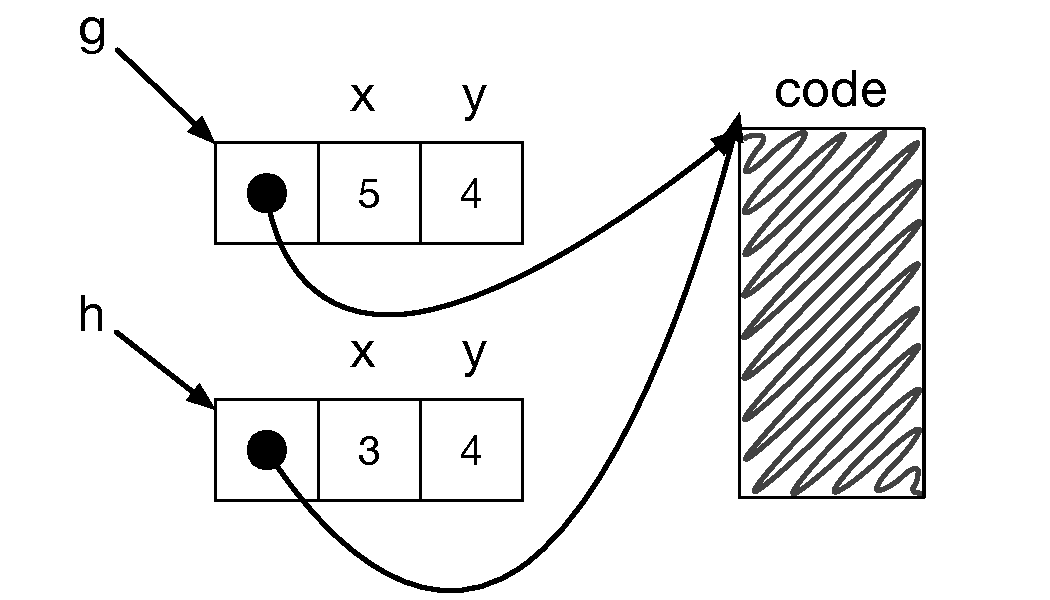
\includegraphics[width=0.6\textwidth]{figs/closures}
\caption{Example closure representation for the \key{lambda}'s
  in Figure~\ref{fig:lexical-scoping}.}
\label{fig:closures}
\end{figure}

Continuing with the example, consider the application of \code{g} to
\code{11} in Figure~\ref{fig:lexical-scoping}.  To apply a closure, we
obtain the function pointer in the first element of the closure and
call it, passing in the closure itself and then the regular arguments,
in this case \code{11}. This technique for applying a closure is step
2 of the dance.
%
But doesn't this \code{lambda} only take 1 argument, for parameter
\code{z}? The third and final step of the dance is generating a
top-level function for a \code{lambda}.  We add an additional
parameter for the closure and we insert a \code{let} at the beginning
of the function for each free variable, to bind those variables to the
appropriate elements from the closure parameter.
%
This three-step dance is known as \emph{closure conversion}.  We
discuss the details of closure conversion in
Section~\ref{sec:closure-conversion} and the code generated from the
example in Section~\ref{sec:example-lambda}. But first we define the
syntax and semantics of $R_5$ in Section~\ref{sec:r5}.

\section{The $R_5$ Language}
\label{sec:r5}

The concrete and abstract syntax for $R_5$, a language with anonymous
functions and lexical scoping, is defined in
Figures~\ref{fig:r5-concrete-syntax} and ~\ref{fig:r5-syntax}. It adds
the \key{lambda} form to the grammar for $R_4$, which already has
syntax for function application.

\begin{figure}[tp]
\centering
\fbox{
  \begin{minipage}{0.96\textwidth}
    \small
\[
\begin{array}{lcl}
  \Type &::=& \gray{\key{Integer} \mid \key{Boolean}
     \mid (\key{Vector}\;\Type\ldots) \mid \key{Void}
     \mid (\Type\ldots \; \key{->}\; \Type)} \\
  \Exp &::=& \gray{\Int \mid (\key{read}) \mid (\key{-}\;\Exp)
     \mid (\key{+} \; \Exp\;\Exp) \mid (\key{-} \; \Exp\;\Exp)}  \\
    &\mid&  \gray{\Var \mid \LET{\Var}{\Exp}{\Exp}}\\
    &\mid& \gray{\key{\#t} \mid \key{\#f} 
     \mid (\key{and}\;\Exp\;\Exp) 
     \mid (\key{or}\;\Exp\;\Exp) 
     \mid (\key{not}\;\Exp) } \\
    &\mid& \gray{(\key{eq?}\;\Exp\;\Exp) \mid \IF{\Exp}{\Exp}{\Exp}} \\
    &\mid& \gray{(\key{vector}\;\Exp\ldots) \mid
          (\key{vector-ref}\;\Exp\;\Int)} \\
    &\mid& \gray{(\key{vector-set!}\;\Exp\;\Int\;\Exp)\mid (\key{void})
     \mid (\Exp \; \Exp\ldots) } \\
    &\mid& (\key{lambda:}\; ([\Var \key{:} \Type]\ldots) \key{:} \Type \; \Exp) \\
  \Def &::=& \gray{(\key{define}\; (\Var \; [\Var \key{:} \Type]\ldots) \key{:} \Type \; \Exp)} \\
  R_5 &::=& \gray{(\key{program} \; \Def\ldots \; \Exp)}
\end{array}
\]
\end{minipage}
}
\caption{Concrete syntax of $R_5$, extending $R_4$ (Figure~\ref{fig:r4-syntax}) 
  with \key{lambda}.}
\label{fig:r5-concrete-syntax}
\end{figure}

\begin{figure}[tp]
\centering
\fbox{
  \begin{minipage}{0.96\textwidth}
    \small
\[
\begin{array}{lcl}
\Exp &::=& \gray{ \INT{\Int} \mid \READ{} \mid \NEG{\Exp} } \\
     &\mid& \gray{ \ADD{\Exp}{\Exp} 
      \mid \BINOP{\code{'-}}{\Exp}{\Exp} } \\
     &\mid& \gray{ \VAR{\Var} \mid \LET{\Var}{\Exp}{\Exp} } \\
     &\mid& \gray{ \BOOL{\itm{bool}} 
      \mid \AND{\Exp}{\Exp} }\\
     &\mid& \gray{ \OR{\Exp}{\Exp}
      \mid \NOT{\Exp} } \\
     &\mid& \gray{ \BINOP{\itm{cmp}}{\Exp}{\Exp}
      \mid \IF{\Exp}{\Exp}{\Exp} } \\
     &\mid& \gray{ \VECTOR{\Exp} } \\
     &\mid& \gray{ \VECREF{\Exp}{\INT{\Int}} }\\
     &\mid& \gray{ \VECSET{\Exp}{\INT{\Int}}{\Exp}} \\
     &\mid& \gray{ \VOID{} \mid \LP\key{HasType}~\Exp~\Type \RP 
     \mid \APPLY{\Exp}{\Exp\ldots} }\\
     &\mid& \LAMBDA{[\Var\code{:}\Type]\ldots}{\Type}{\Exp}\\
 \Def &::=& \gray{ \FUNDEF{\Var}{([\Var \code{:} \Type]\ldots)}{\Type}{\code{'()}}{\Exp} }\\
  R_5 &::=& \gray{ \PROGRAMDEFSEXP{\code{'()}}{(\Def\ldots)}{\Exp} }
\end{array}
\]
\end{minipage}
}
\caption{The abstract syntax of $R_5$, extending $R_4$ (Figure~\ref{fig:r4-syntax}).}
\label{fig:r5-syntax}
\end{figure}

\index{interpreter}
\label{sec:interp-R5}

Figure~\ref{fig:interp-R5} shows the definitional interpreter for
$R_5$. The clause for \key{lambda} saves the current environment
inside the returned \key{lambda}. Then the clause for \key{Apply} uses
the environment from the \key{lambda}, the \code{lam-env}, when
interpreting the body of the \key{lambda}.  The \code{lam-env}
environment is extended with the mapping of parameters to argument
values.

\begin{figure}[tbp]
\begin{lstlisting}
(define (interp-exp env)
  (lambda (e)
    (define recur (interp-exp env))
    (match e
      ...
      [(Lambda (list `[,xs : ,Ts] ...) rT body)
       `(lambda ,xs ,body ,env)]
      [(Apply fun args)
       (define fun-val ((interp-exp env) fun))
       (define arg-vals (map (interp-exp env) args))
       (match fun-val
	 [`(lambda ,xs ,body ,lam-env)
	  (define new-env (append (map cons xs arg-vals) lam-env))
	  ((interp-exp new-env) body)]
	 [else (error "interp-exp, expected function, not" fun-val)])]
      [else (error 'interp-exp "unrecognized expression")]
      )))
\end{lstlisting}
\caption{Interpreter for $R_5$.}
\label{fig:interp-R5}
\end{figure}


\label{sec:type-check-r5}
\index{type checking}

Figure~\ref{fig:type-check-R5} shows how to type check the new
\key{lambda} form. The body of the \key{lambda} is checked in an
environment that includes the current environment (because it is
lexically scoped) and also includes the \key{lambda}'s parameters.  We
require the body's type to match the declared return type.

\begin{figure}[tbp]
\begin{lstlisting}
(define (type-check-R5 env)
  (lambda (e)
    (match e
      [(Lambda (and bnd `([,xs : ,Ts] ...)) rT body)
       (define-values (new-body bodyT) 
          ((type-check-exp (append (map cons xs Ts) env)) body))
       (define ty `(,@Ts -> ,rT))
       (cond
         [(equal? rT bodyT)
           (values (HasType (Lambda bnd rT new-body) ty) ty)]
         [else
           (error "mismatch in return type" bodyT rT)])]
      ...
      )))
\end{lstlisting}
\caption{Type checking the \key{lambda}'s in $R_5$.}
\label{fig:type-check-R5}
\end{figure}


\section{Closure Conversion}
\label{sec:closure-conversion}
\index{closure conversion}

The compiling of lexically-scoped functions into top-level function
definitions is accomplished in the pass \code{convert-to-closures}
that comes after \code{reveal-functions} and before
\code{limit-functions}. 

As usual, we implement the pass as a recursive function over the
AST. All of the action is in the clauses for \key{lambda} and
\key{Apply}. We transform a \key{lambda} expression into an expression
that creates a closure, that is, creates a vector whose first element
is a function pointer and the rest of the elements are the free
variables of the \key{lambda}.  The \itm{name} is a unique symbol
generated to identify the function.

\begin{tabular}{lll}
\begin{minipage}{0.4\textwidth}
\begin{lstlisting}
(lambda: (|\itm{ps}| ...) : |\itm{rt}| |\itm{body}|)
\end{lstlisting}
\end{minipage}
&
$\Rightarrow$
&
\begin{minipage}{0.4\textwidth}
\begin{lstlisting}
(vector |\itm{name}| |\itm{fvs}| ...)
\end{lstlisting}
\end{minipage}
\end{tabular}  \\
%
In addition to transforming each \key{lambda} into a \key{vector}, we
must create a top-level function definition for each \key{lambda}, as
shown below.\\
\begin{minipage}{0.8\textwidth}
  \begin{lstlisting}
   (define (|\itm{name}| [clos : (Vector _ |\itm{fvts}| ...)] |\itm{ps}| ...)
      (let ([|$\itm{fvs}_1$| (vector-ref clos 1)])
        ...
        (let ([|$\itm{fvs}_n$| (vector-ref clos |$n$|)])
          |\itm{body'}|)...))
\end{lstlisting}
\end{minipage}\\
The \code{clos} parameter refers to the closure. The $\itm{ps}$
parameters are the normal parameters of the \key{lambda}. The types
$\itm{fvts}$ are the types of the free variables in the lambda and the
underscore is a dummy type because it is rather difficult to give a
type to the function in the closure's type, and it does not matter.
The sequence of \key{let} forms bind the free variables to their
values obtained from the closure.

We transform function application into code that retrieves the
function pointer from the closure and then calls the function, passing
in the closure as the first argument. We bind $e'$ to a temporary
variable to avoid code duplication.

\begin{tabular}{lll}
\begin{minipage}{0.3\textwidth}
\begin{lstlisting}
(app |$e$| |\itm{es}| ...)
\end{lstlisting}
\end{minipage}
&
$\Rightarrow$
&
\begin{minipage}{0.5\textwidth}
\begin{lstlisting}
(let ([|\itm{tmp}| |$e'$|])
  (app (vector-ref |\itm{tmp}| 0) |\itm{tmp}| |\itm{es'}|))
\end{lstlisting}
\end{minipage}
\end{tabular}  \\

There is also the question of what to do with top-level function
definitions. To maintain a uniform translation of function
application, we turn function references into closures.

\begin{tabular}{lll}
\begin{minipage}{0.3\textwidth}
\begin{lstlisting}
(fun-ref |$f$|)
\end{lstlisting}
\end{minipage}
&
$\Rightarrow$
&
\begin{minipage}{0.5\textwidth}
\begin{lstlisting}
(vector (fun-ref |$f$|))
\end{lstlisting}
\end{minipage}
\end{tabular}  \\
%
The top-level function definitions need to be updated as well to take
an extra closure parameter.

\section{An Example Translation}
\label{sec:example-lambda}

Figure~\ref{fig:lexical-functions-example} shows the result of closure
conversion for the example program demonstrating lexical scoping that
we discussed at the beginning of this chapter.


\begin{figure}[h]
\begin{minipage}{0.8\textwidth}
\begin{lstlisting}%[basicstyle=\ttfamily\footnotesize]
(program
 (define (f [x : Integer]) : (Integer -> Integer)
    (let ([y 4])
       (lambda: ([z : Integer]) : Integer
          (+ x (+ y z)))))
 (let ([g (f 5)])
   (let ([h (f 3)])
     (+ (g 11) (h 15)))))
\end{lstlisting}
$\Downarrow$
\begin{lstlisting}%[basicstyle=\ttfamily\footnotesize]
(program (type Integer)
  (define (f (x : Integer)) : (Integer -> Integer)
    (let ((y 4))
       (lambda: ((z : Integer)) : Integer
         (+ x (+ y z)))))
   (let ((g (app (fun-ref f) 5)))
      (let ((h (app (fun-ref f) 3)))
         (+ (app g 11) (app h 15)))))
\end{lstlisting}
$\Downarrow$
\begin{lstlisting}%[basicstyle=\ttfamily\footnotesize]
(program (type Integer)
  (define (f (clos.1 : _) (x : Integer)) : (Integer -> Integer)
     (let ((y 4))
        (vector (fun-ref lam.1) x y)))
  (define (lam.1 (clos.2 : _) (z : Integer)) : Integer
     (let ((x (vector-ref clos.2 1)))
        (let ((y (vector-ref clos.2 2)))
           (+ x (+ y z)))))
   (let ((g (let ((t.1 (vector (fun-ref f))))
              (app (vector-ref t.1 0) t.1 5))))
      (let ((h (let ((t.2 (vector  (fun-ref f))))
                 (app (vector-ref t.2 0) t.2 3))))
         (+ (let ((t.3 g)) (app (vector-ref t.3 0) t.3 11))
            (let ((t.4 h)) (app (vector-ref t.4 0) t.4 15))))))
\end{lstlisting}
\end{minipage}

\caption{Example of closure conversion.}
\label{fig:lexical-functions-example}
\end{figure}



\begin{figure}[p]
\begin{tikzpicture}[baseline=(current  bounding  box.center)]
\node (R4) at (0,2)  {\large $R_4$};
\node (R4-2) at (3,2)  {\large $R_4$};
\node (R4-3) at (6,2)  {\large $R_4$};
\node (F1-1) at (12,0)  {\large $F_1$};
\node (F1-2) at (9,0)  {\large $F_1$};
\node (F1-3) at (6,0)  {\large $F_1$};
\node (F1-4) at (3,0)  {\large $F_1$};
\node (F1-5) at (0,0)  {\large $F_1$};
\node (C3-1) at (6,-2)  {\large $C_3$};
\node (C3-2) at (3,-2)  {\large $C_3$};

\node (x86-2) at (3,-4)  {\large $\text{x86}^{*}_3$};
\node (x86-3) at (6,-4)  {\large $\text{x86}^{*}_3$};
\node (x86-4) at (9,-4) {\large $\text{x86}^{*}_3$};
\node (x86-5) at (9,-6) {\large $\text{x86}^{\dagger}_3$};

\node (x86-2-1) at (3,-6)  {\large $\text{x86}^{*}_3$};
\node (x86-2-2) at (6,-6)  {\large $\text{x86}^{*}_3$};

\path[->,bend left=15] (R4) edge [above] node
     {\ttfamily\footnotesize\color{red} type-check} (R4-2);
\path[->,bend left=15] (R4-2) edge [above] node
     {\ttfamily\footnotesize uniquify} (R4-3);
\path[->] (R4-3) edge [right] node
     {\ttfamily\footnotesize reveal-functions} (F1-1);
\path[->,bend left=15] (F1-1) edge [below] node
     {\ttfamily\footnotesize\color{red} convert-to-clos.} (F1-2);
\path[->,bend right=15] (F1-2) edge [above] node
     {\ttfamily\footnotesize limit-functions} (F1-3);
\path[->,bend right=15] (F1-3) edge [above] node
     {\ttfamily\footnotesize expose-alloc.} (F1-4);
\path[->,bend right=15] (F1-4) edge [above] node
     {\ttfamily\footnotesize remove-complex.} (F1-5);
\path[->] (F1-5) edge [left] node
     {\ttfamily\footnotesize explicate-control} (C3-1);
\path[->,bend left=15] (C3-1) edge [below] node
     {\ttfamily\footnotesize uncover-locals} (C3-2);
\path[->,bend right=15] (C3-2) edge [left] node
     {\ttfamily\footnotesize select-instr.} (x86-2);
\path[->,bend left=15] (x86-2) edge [left] node
     {\ttfamily\footnotesize uncover-live} (x86-2-1);
\path[->,bend right=15] (x86-2-1) edge [below] node 
     {\ttfamily\footnotesize build-inter.} (x86-2-2);
\path[->,bend right=15] (x86-2-2) edge [left] node
     {\ttfamily\footnotesize allocate-reg.} (x86-3);
\path[->,bend left=15] (x86-3) edge [above] node
     {\ttfamily\footnotesize patch-instr.} (x86-4);
\path[->,bend right=15] (x86-4) edge [left] node {\ttfamily\footnotesize print-x86} (x86-5);
\end{tikzpicture}
  \caption{Diagram of the passes for $R_5$, a language with lexically-scoped
  functions.}
\label{fig:R5-passes}
\end{figure}

Figure~\ref{fig:R5-passes} provides an overview of all the passes needed
for the compilation of $R_5$.

\begin{exercise}\normalfont
Expand your compiler to handle $R_5$ as outlined in this chapter.
Create 5 new programs that use \key{lambda} functions and make use of
lexical scoping. Test your compiler on these new programs and all of
your previously created test programs.
\end{exercise}


%%%%%%%%%%%%%%%%%%%%%%%%%%%%%%%%%%%%%%%%%%%%%%%%%%%%%%%%%%%%%%%%%%%%%%%%%%%%%%%%
\chapter{Dynamic Typing}
\label{ch:type-dynamic}
\index{dynamic typing}

In this chapter we discuss the compilation of a dynamically typed
language, named $R_7$, that is a subset of the Racket
language. (Recall that in the previous chapters we have studied
subsets of the \emph{Typed} Racket language.) In dynamically typed
languages, an expression may produce values of differing
type. Consider the following example with a conditional expression
that may return a Boolean or an integer depending on the input to the
program.
\begin{lstlisting}
   (not (if (eq? (read) 1) #f 0))
\end{lstlisting}
Languages that allow expressions to produce different kinds of values
are called \emph{polymorphic}. There are many kinds of polymorphism,
such as subtype polymorphism and parametric
polymorphism~\citep{Cardelli:1985kx}. The kind of polymorphism we are
talking about here does not have a special name, but it is the usual
kind that arises in dynamically typed languages.

Another characteristic of dynamically typed languages is that
primitive operations, such as \code{not}, are often defined to operate
on many different types of values. In fact, in Racket, the \code{not}
operator produces a result for any kind of value: given \code{\#f} it
returns \code{\#t} and given anything else it returns \code{\#f}.
Furthermore, even when primitive operations restrict their inputs to
values of a certain type, this restriction is enforced at runtime
instead of during compilation. For example, the following vector
reference results in a run-time contract violation.
\begin{lstlisting}
   (vector-ref (vector 42) #t)
\end{lstlisting}

\begin{figure}[tp]
\centering
\fbox{
\begin{minipage}{0.97\textwidth}
\[
\begin{array}{rcl}
  \itm{cmp} &::= & \key{eq?} \mid \key{<} \mid \key{<=} \mid \key{>} \mid \key{>=} \\
\Exp &::=& \Int \mid (\key{read}) \mid (\key{-}\;\Exp) 
      \mid (\key{+} \; \Exp\;\Exp) \mid (\key{-} \; \Exp\;\Exp)  \\
     &\mid&  \Var \mid \LET{\Var}{\Exp}{\Exp} \\
     &\mid& \key{\#t} \mid \key{\#f} 
      \mid (\key{and}\;\Exp\;\Exp) 
      \mid (\key{or}\;\Exp\;\Exp) 
      \mid (\key{not}\;\Exp) \\
     &\mid& (\itm{cmp}\;\Exp\;\Exp) \mid \IF{\Exp}{\Exp}{\Exp} \\
     &\mid& (\key{vector}\;\Exp\ldots) \mid
      (\key{vector-ref}\;\Exp\;\Exp) \\
     &\mid& (\key{vector-set!}\;\Exp\;\Exp\;\Exp) \mid (\key{void}) \\
     &\mid& (\Exp \; \Exp\ldots) \mid (\key{lambda}\; (\Var\ldots) \; \Exp) \\
     & \mid & (\key{boolean?}\;\Exp) \mid (\key{integer?}\;\Exp)\\
     & \mid & (\key{vector?}\;\Exp) \mid (\key{procedure?}\;\Exp) \mid (\key{void?}\;\Exp) \\
  \Def &::=& (\key{define}\; (\Var \; \Var\ldots) \; \Exp) \\
R_7  &::=& (\key{program} \; \Def\ldots\; \Exp)
\end{array}
\]
\end{minipage}
}
\caption{Syntax of $R_7$, an untyped language (a subset of Racket).}
\label{fig:r7-syntax}
\end{figure}

The syntax of $R_7$, our subset of Racket, is defined in
Figure~\ref{fig:r7-syntax}.
%
The definitional interpreter for $R_7$ is given in
Figure~\ref{fig:interp-R7}.

\begin{figure}[tbp]
\begin{lstlisting}[basicstyle=\ttfamily\footnotesize]
(define (get-tagged-type v) (match v [`(tagged ,v1 ,ty) ty]))

(define (valid-op? op) (member op '(+ - and or not)))

(define (interp-r7 env)
  (lambda (ast)
    (define recur (interp-r7 env))
    (match ast
      [(? symbol?) (lookup ast env)]
      [(? integer?) `(inject ,ast Integer)]
      [#t `(inject #t Boolean)]
      [#f `(inject #f Boolean)]
      [`(read) `(inject ,(read-fixnum) Integer)]
      [`(lambda (,xs ...) ,body)
       `(inject (lambda ,xs ,body ,env) (,@(map (lambda (x) 'Any) xs) -> Any))]
      [`(define (,f ,xs ...) ,body)
       (mcons f `(lambda ,xs ,body))]
      [`(program ,ds ... ,body)
       (let ([top-level (for/list ([d ds]) ((interp-r7 '()) d))])
         (for/list ([b top-level])
           (set-mcdr! b (match (mcdr b)
                          [`(lambda ,xs ,body)
                           `(inject (lambda ,xs ,body ,top-level)
                                    (,@(map (lambda (x) 'Any) xs) -> Any))])))
         ((interp-r7 top-level) body))]
      [`(vector ,(app recur elts) ...)
       (define tys (map get-tagged-type elts))
       `(inject ,(apply vector elts) (Vector ,@tys))]
      [`(vector-set! ,(app recur v1) ,n ,(app recur v2))
         (match v1
           [`(inject ,vec ,ty)
             (vector-set! vec n v2)
            `(inject (void) Void)])]
      [`(vector-ref ,(app recur v) ,n)
       (match v [`(inject ,vec ,ty) (vector-ref vec n)])]
      [`(let ([,x ,(app recur v)]) ,body)
       ((interp-r7 (cons (cons x v) env)) body)]
      [`(,op ,es ...) #:when (valid-op? op)
       (interp-r7-op op (for/list ([e es]) (recur e)))]
      [`(eq? ,(app recur l) ,(app recur r))
       `(inject ,(equal? l r) Boolean)]
      [`(if ,(app recur q) ,t ,f)
       (match q
         [`(inject #f Boolean) (recur f)]
         [else (recur t)])]
      [`(,(app recur f-val) ,(app recur vs) ...)
       (match f-val
         [`(inject (lambda (,xs ...) ,body ,lam-env) ,ty)
          (define new-env (append (map cons xs vs) lam-env))
          ((interp-r7 new-env) body)]
         [else (error "interp-r7, expected function, not" f-val)])])))
\end{lstlisting}
\caption{Interpreter for the $R_7$ language. UPDATE ME -Jeremy}
\label{fig:interp-R7}
\end{figure}


Let us consider how we might compile $R_7$ to x86, thinking about the
first example above. Our bit-level representation of the Boolean
\code{\#f} is zero and similarly for the integer \code{0}.  However,
\code{(not \#f)} should produce \code{\#t} whereas \code{(not 0)}
should produce \code{\#f}. Furthermore, the behavior of \code{not}, in
general, cannot be determined at compile time, but depends on the
runtime type of its input, as in the example above that depends on the
result of \code{(read)}.

The way around this problem is to include information about a value's
runtime type in the value itself, so that this information can be
inspected by operators such as \code{not}.  In particular, we 
steal the 3 right-most bits from our 64-bit values to encode the
runtime type.  We use $001$ to identify integers, $100$ for
Booleans, $010$ for vectors, $011$ for procedures, and $101$ for the
void value. We refer to these 3 bits as the \emph{tag} and we
define the following auxiliary function.
\begin{align*}
\itm{tagof}(\key{Integer}) &= 001 \\
\itm{tagof}(\key{Boolean}) &= 100 \\
\itm{tagof}((\key{Vector} \ldots)) &= 010 \\
\itm{tagof}((\key{Vectorof} \ldots)) &= 010 \\
\itm{tagof}((\ldots \key{->} \ldots)) &= 011 \\
\itm{tagof}(\key{Void}) &= 101
\end{align*}
(We say more about the new \key{Vectorof} type shortly.)
This stealing of 3 bits comes at some
price: our integers are reduced to ranging from $-2^{60}$ to
$2^{60}$. The stealing does not adversely affect vectors and
procedures because those values are addresses, and our addresses are
8-byte aligned so the rightmost 3 bits are unused, they are always
$000$. Thus, we do not lose information by overwriting the rightmost 3
bits with the tag and we can simply zero-out the tag to recover the
original address.

In some sense, these tagged values are a new kind of value.  Indeed,
we can extend our \emph{typed} language with tagged values by adding a
new type to classify them, called \key{Any}, and with operations for
creating and using tagged values, yielding the $R_6$ language that we
define in Section~\ref{sec:r6-lang}. The $R_6$ language provides the
fundamental support for polymorphism and runtime types that we need to
support dynamic typing.

There is an interesting interaction between tagged values and garbage
collection.  A variable of type \code{Any} might refer to a vector and
therefore it might be a root that needs to be inspected and copied
during garbage collection. Thus, we need to treat variables of type
\code{Any} in a similar way to variables of type \code{Vector} for
purposes of register allocation, which we discuss in
Section~\ref{sec:register-allocation-r6}. One concern is that, if a
variable of type \code{Any} is spilled, it must be spilled to the root
stack.  But this means that the garbage collector needs to be able to
differentiate between (1) plain old pointers to tuples, (2) a tagged
value that points to a tuple, and (3) a tagged value that is not a
tuple. We enable this differentiation by choosing not to use the tag
$000$. Instead, that bit pattern is reserved for identifying plain old
pointers to tuples. On the other hand, if one of the first three bits
is set, then we have a tagged value, and inspecting the tag can
differentiation between vectors ($010$) and the other kinds of values.

We implement our untyped language $R_7$ by compiling it to $R_6$
(Section~\ref{sec:compile-r7}), but first we describe the how to
extend our compiler to handle the new features of $R_6$
(Sections~\ref{sec:shrink-r6}, \ref{sec:select-r6}, and
\ref{sec:register-allocation-r6}).

\section{The $R_6$ Language: Typed Racket $+$ \key{Any}}
\label{sec:r6-lang}

\begin{figure}[tp]
\centering
\fbox{
\begin{minipage}{0.97\textwidth}
\[
\begin{array}{lcl}
  \Type &::=& \gray{\key{Integer} \mid \key{Boolean}
     \mid (\key{Vector}\;\Type\ldots) \mid (\key{Vectorof}\;\Type) \mid \key{Void}} \\
    &\mid& \gray{(\Type\ldots \; \key{->}\; \Type)} \mid \key{Any} \\
  \FType &::=& \key{Integer} \mid \key{Boolean} \mid \key{Void} \mid (\key{Vectorof}\;\key{Any}) \mid (\key{Vector}\; \key{Any}\ldots) \\
    &\mid& (\key{Any}\ldots \; \key{->}\; \key{Any})\\
  \itm{cmp} &::= & \key{eq?} \mid \key{<} \mid \key{<=} \mid \key{>} \mid \key{>=} \\
  \Exp &::=& \gray{\Int \mid (\key{read}) \mid (\key{-}\;\Exp)
     \mid (\key{+} \; \Exp\;\Exp) \mid (\key{-} \; \Exp\;\Exp)}  \\
    &\mid&  \gray{\Var \mid \LET{\Var}{\Exp}{\Exp}} \\
    &\mid& \gray{\key{\#t} \mid \key{\#f} 
     \mid (\key{and}\;\Exp\;\Exp) 
     \mid (\key{or}\;\Exp\;\Exp) 
     \mid (\key{not}\;\Exp)} \\
    &\mid& \gray{(\itm{cmp}\;\Exp\;\Exp) \mid \IF{\Exp}{\Exp}{\Exp}} \\
    &\mid& \gray{(\key{vector}\;\Exp\ldots) \mid
          (\key{vector-ref}\;\Exp\;\Int)} \\
    &\mid& \gray{(\key{vector-set!}\;\Exp\;\Int\;\Exp)\mid (\key{void})} \\
    &\mid& \gray{(\Exp \; \Exp\ldots)
    \mid (\key{lambda:}\; ([\Var \key{:} \Type]\ldots) \key{:} \Type \; \Exp)} \\
  & \mid & (\key{inject}\; \Exp \; \FType) \mid (\key{project}\;\Exp\;\FType) \\
  & \mid & (\key{boolean?}\;\Exp) \mid (\key{integer?}\;\Exp)\\
  & \mid & (\key{vector?}\;\Exp) \mid (\key{procedure?}\;\Exp) \mid (\key{void?}\;\Exp) \\
  \Def &::=& \gray{(\key{define}\; (\Var \; [\Var \key{:} \Type]\ldots) \key{:} \Type \; \Exp)} \\
  R_6 &::=& \gray{(\key{program} \; \Def\ldots \; \Exp)}
\end{array}
\]
\end{minipage}
}
\caption{Syntax of $R_6$, extending $R_5$ (Figure~\ref{fig:r5-syntax})
  with \key{Any}.}
\label{fig:r6-syntax}
\end{figure}

The syntax of $R_6$ is defined in Figure~\ref{fig:r6-syntax}.  The
$(\key{inject}\; e\; T)$ form converts the value produced by
expression $e$ of type $T$ into a tagged value.  The
$(\key{project}\;e\;T)$ form converts the tagged value produced by
expression $e$ into a value of type $T$ or else halts the program if
the type tag is equivalent to $T$. We treat
$(\key{Vectorof}\;\key{Any})$ as equivalent to
$(\key{Vector}\;\key{Any}\;\ldots)$.

Note that in both \key{inject} and
\key{project}, the type $T$ is restricted to the flat types $\FType$,
which simplifies the implementation and corresponds with what is
needed for compiling untyped Racket. The type predicates,
$(\key{boolean?}\,e)$ etc., expect a tagged value and return \key{\#t}
if the tag corresponds to the predicate, and return \key{\#t}
otherwise.
%
Selections from the type checker for $R_6$ are shown in
Figure~\ref{fig:type-check-R6} and the interpreter for $R_6$ is in
Figure~\ref{fig:interp-R6}.

\begin{figure}[btp]
\begin{lstlisting}[basicstyle=\ttfamily\footnotesize]
(define (flat-ty? ty) ...)

(define (type-check-R6 env)
  (lambda (e)
    (define recur (type-check-R6 env))
    (match e
       [`(inject ,e ,ty)
        (unless (flat-ty? ty)
          (error "may only inject a value of flat type, not ~a" ty))
        (define-values (new-e e-ty) (recur e))
        (cond
         [(equal? e-ty ty)
          (values `(inject ,new-e ,ty) 'Any)]
         [else
          (error "inject expected ~a to have type ~a" e ty)])]
       [`(project ,e ,ty)
        (unless (flat-ty? ty)
          (error "may only project to a flat type, not ~a" ty))
        (define-values (new-e e-ty) (recur e))
        (cond
         [(equal? e-ty 'Any)
          (values `(project ,new-e ,ty) ty)]
         [else
          (error "project expected ~a to have type Any" e)])]
       [`(vector-ref ,e ,i)
        (define-values (new-e e-ty) (recur e))
        (match e-ty
          [`(Vector ,ts ...) ...]
          [`(Vectorof ,ty)
           (unless (exact-nonnegative-integer? i)
             (error 'type-check "invalid index ~a" i))
           (values `(vector-ref ,new-e ,i) ty)]
          [else (error "expected a vector in vector-ref, not" e-ty)])]
        ...
      )))
\end{lstlisting}
\caption{Type checker for parts of the $R_6$ language.}
\label{fig:type-check-R6}
\end{figure}

% to do: add rules for vector-ref, etc. for Vectorof
%Also, \key{eq?} is extended to operate on values of type \key{Any}.

\begin{figure}[btp]
\begin{lstlisting}
(define primitives (set 'boolean? ...))

(define (interp-op op)
  (match op
     ['boolean? (lambda (v)
                  (match v
                     [`(tagged ,v1 Boolean) #t]
                     [else #f]))]
     ...))

;; Equivalence of flat types
(define (tyeq? t1 t2)
  (match `(,t1 ,t2)
    [`((Vectorof Any) (Vector ,t2s ...))
     (for/and ([t2 t2s]) (eq? t2 'Any))]
    [`((Vector ,t1s ...) (Vectorof Any))
     (for/and ([t1 t1s]) (eq? t1 'Any))]
    [else (equal? t1 t2)]))

(define (interp-R6 env)
  (lambda (ast)
    (match ast
       [`(inject ,e ,t)
        `(tagged ,((interp-R6 env) e) ,t)]
       [`(project ,e ,t2)
        (define v ((interp-R6 env) e))
        (match v
           [`(tagged ,v1 ,t1)
            (cond [(tyeq? t1 t2)
                   v1]
                  [else
                   (error "in project, type mismatch" t1 t2)])]
           [else
            (error "in project, expected tagged value" v)])]
       ...)))
\end{lstlisting}
\caption{Interpreter for $R_6$.}
\label{fig:interp-R6}
\end{figure}

%\clearpage

\section{Shrinking $R_6$}
\label{sec:shrink-r6}

In the \code{shrink} pass we recommend compiling \code{project} into
an explicit \code{if} expression that uses three new operations:
\code{tag-of-any}, \code{value-of-any}, and \code{exit}.  The
\code{tag-of-any} operation retrieves the type tag from a tagged value
of type \code{Any}.  The \code{value-of-any} retrieves the underlying
value from a tagged value. Finally, the \code{exit} operation ends the
execution of the program by invoking the operating system's
\code{exit} function. So the translation for \code{project} is as
follows. (We have omitted the \code{has-type} AST nodes to make this
output more readable.)

\begin{tabular}{lll}
\begin{minipage}{0.3\textwidth}
\begin{lstlisting}
   (project |$e$| |$\Type$|)
\end{lstlisting}
\end{minipage}
&
$\Rightarrow$
&
\begin{minipage}{0.5\textwidth}
\begin{lstlisting}
(let ([|$\itm{tmp}$| |$e'$|])
  (if (eq? (tag-of-any |$\itm{tmp}$|) |$\itm{tag}$|)
      (value-of-any |$\itm{tmp}$|)
      (exit)))
\end{lstlisting}
\end{minipage}
\end{tabular}  \\

Similarly, we recommend translating the type predicates
(\code{boolean?}, etc.) into uses of \code{tag-of-any} and \code{eq?}.

\section{Instruction Selection for $R_6$}
\label{sec:select-r6}

\paragraph{Inject}

We recommend compiling an \key{inject} as follows if the type is
\key{Integer} or \key{Boolean}.  The \key{salq} instruction shifts the
destination to the left by the number of bits specified its source
argument (in this case $3$, the length of the tag) and it preserves
the sign of the integer. We use the \key{orq} instruction to combine
the tag and the value to form the tagged value.  \\
\begin{tabular}{lll}
\begin{minipage}{0.4\textwidth}
\begin{lstlisting}
(assign |\itm{lhs}| (inject |$e$| |$T$|))
\end{lstlisting}
\end{minipage}
&
$\Rightarrow$
&
\begin{minipage}{0.5\textwidth}
\begin{lstlisting}
(movq |$e'$| |\itm{lhs}'|)
(salq (int 3) |\itm{lhs}'|)
(orq (int |$\itm{tagof}(T)$|) |\itm{lhs}'|)
\end{lstlisting}
\end{minipage}
\end{tabular}  \\
The instruction selection for vectors and procedures is different
because their is no need to shift them to the left. The rightmost 3
bits are already zeros as described above. So we just combine the
value and the tag using \key{orq}.  \\
\begin{tabular}{lll}
\begin{minipage}{0.4\textwidth}
\begin{lstlisting}
(assign |\itm{lhs}| (inject |$e$| |$T$|))
\end{lstlisting}
\end{minipage}
&
$\Rightarrow$
&
\begin{minipage}{0.5\textwidth}
\begin{lstlisting}
(movq |$e'$| |\itm{lhs}'|)
(orq (int |$\itm{tagof}(T)$|) |\itm{lhs}'|)
\end{lstlisting}
\end{minipage}
\end{tabular} 

\paragraph{Tag of Any}

Recall that the \code{tag-of-any} operation extracts the type tag from
a value of type \code{Any}. The type tag is the bottom three bits, so
we obtain the tag by taking the bitwise-and of the value with $111$
($7$ in decimal).

\begin{tabular}{lll}
\begin{minipage}{0.4\textwidth}
\begin{lstlisting}
(assign |\itm{lhs}| (tag-of-any |$e$|))
\end{lstlisting}
\end{minipage}
&
$\Rightarrow$
&
\begin{minipage}{0.5\textwidth}
\begin{lstlisting}
(movq |$e'$| |\itm{lhs}'|)
(andq (int 7) |\itm{lhs}'|)
\end{lstlisting}
\end{minipage}
\end{tabular}  

\paragraph{Value of Any}

Like \key{inject}, the instructions for \key{value-of-any} are
different depending on whether the type $T$ is a pointer (vector or
procedure) or not (Integer or Boolean). The following shows the
instruction selection for Integer and Boolean.  We produce an untagged
value by shifting it to the right by 3 bits.
%
\\
\begin{tabular}{lll}
\begin{minipage}{0.4\textwidth}
\begin{lstlisting}
(assign |\itm{lhs}| (project |$e$| |$T$|))
\end{lstlisting}
\end{minipage}
&
$\Rightarrow$
&
\begin{minipage}{0.5\textwidth}
\begin{lstlisting}
(movq |$e'$| |\itm{lhs}'|)
(sarq (int 3) |\itm{lhs}'|)
\end{lstlisting}
\end{minipage}
\end{tabular}  \\
%
In the case for vectors and procedures, there is no need to
shift. Instead we just need to zero-out the rightmost 3 bits. We
accomplish this by creating the bit pattern $\ldots 0111$ ($7$ in
decimal) and apply \code{bitwise-not} to obtain $\ldots 1000$ which we
\code{movq} into the destination $\itm{lhs}$.  We then generate
\code{andq} with the tagged value to get the desired result. \\
%
\begin{tabular}{lll}
\begin{minipage}{0.4\textwidth}
\begin{lstlisting}
(assign |\itm{lhs}| (project |$e$| |$T$|))
\end{lstlisting}
\end{minipage}
&
$\Rightarrow$
&
\begin{minipage}{0.5\textwidth}
\begin{lstlisting}
(movq (int |$\ldots 1000$|) |\itm{lhs}'|)
(andq |$e'$| |\itm{lhs}'|)
\end{lstlisting}
\end{minipage}
\end{tabular}  

%% \paragraph{Type Predicates} We leave it to the reader to
%% devise a sequence of instructions to implement the type predicates
%% \key{boolean?}, \key{integer?}, \key{vector?}, and \key{procedure?}.

\section{Register Allocation for $R_6$}
\label{sec:register-allocation-r6}
\index{register allocation}

As mentioned above, a variable of type \code{Any} might refer to a
vector. Thus, the register allocator for $R_6$ needs to treat variable
of type \code{Any} in the same way that it treats variables of type
\code{Vector} for purposes of garbage collection. In particular,
\begin{itemize}
\item If a variable of type \code{Any} is live during a function call,
  then it must be spilled. One way to accomplish this is to augment
  the pass \code{build-interference} to mark all variables that are
  live after a \code{callq} as interfering with all the registers.

\item If a variable of type \code{Any} is spilled, it must be spilled
  to the root stack instead of the normal procedure call stack.
\end{itemize}

\begin{exercise}\normalfont
Expand your compiler to handle $R_6$ as discussed in the last few
sections.  Create 5 new programs that use the \code{Any} type and the
new operations (\code{inject}, \code{project}, \code{boolean?},
etc.). Test your compiler on these new programs and all of your
previously created test programs.
\end{exercise}

\section{Compiling $R_7$ to $R_6$}
\label{sec:compile-r7}

Figure~\ref{fig:compile-r7-r6} shows the compilation of many of the
$R_7$ forms into $R_6$. An important invariant of this pass is that
given a subexpression $e$ of $R_7$, the pass will produce an
expression $e'$ of $R_6$ that has type \key{Any}. For example, the
first row in Figure~\ref{fig:compile-r7-r6} shows the compilation of
the Boolean \code{\#t}, which must be injected to produce an
expression of type \key{Any}.
%
The second row of Figure~\ref{fig:compile-r7-r6}, the compilation of
addition, is representative of compilation for many operations: the
arguments have type \key{Any} and must be projected to \key{Integer}
before the addition can be performed.

The compilation of \key{lambda} (third row of
Figure~\ref{fig:compile-r7-r6}) shows what happens when we need to
produce type annotations: we simply use \key{Any}.
%
The compilation of \code{if} and \code{eq?}  demonstrate how this pass
has to account for some differences in behavior between $R_7$ and
$R_6$. The $R_7$ language is more permissive than $R_6$ regarding what
kind of values can be used in various places. For example, the
condition of an \key{if} does not have to be a Boolean. For \key{eq?},
the arguments need not be of the same type (but in that case, the
result will be \code{\#f}).

\begin{figure}[btp]
\centering
\begin{tabular}{|lll|} \hline
\begin{minipage}{0.25\textwidth}
\begin{lstlisting}
#t
\end{lstlisting}
\end{minipage}
&
$\Rightarrow$
&
\begin{minipage}{0.6\textwidth}
\begin{lstlisting}
(inject #t Boolean)
\end{lstlisting}
\end{minipage}
\\[2ex]\hline
\begin{minipage}{0.25\textwidth}
\begin{lstlisting}
(+ |$e_1$| |$e_2$|)
\end{lstlisting}
\end{minipage}
&
$\Rightarrow$
&
\begin{minipage}{0.6\textwidth}
\begin{lstlisting}
(inject
   (+ (project |$e'_1$| Integer)
      (project |$e'_2$| Integer))
   Integer)
\end{lstlisting}
\end{minipage}
\\[2ex]\hline
\begin{minipage}{0.25\textwidth}
\begin{lstlisting}
(lambda (|$x_1 \ldots$|) |$e$|)
\end{lstlisting}
\end{minipage}
&
$\Rightarrow$
&
\begin{minipage}{0.6\textwidth}
\begin{lstlisting}
(inject (lambda: ([|$x_1$|:Any]|$\ldots$|):Any |$e'$|)
        (Any|$\ldots$|Any -> Any))
\end{lstlisting}
\end{minipage}
\\[2ex]\hline
\begin{minipage}{0.25\textwidth}
\begin{lstlisting}
(app |$e_0$| |$e_1 \ldots e_n$|)
\end{lstlisting}
\end{minipage}
&
$\Rightarrow$
&
\begin{minipage}{0.6\textwidth}
\begin{lstlisting}
(app (project |$e'_0$| (Any|$\ldots$|Any -> Any))
   |$e'_1 \ldots e'_n$|)
\end{lstlisting}
\end{minipage}
\\[2ex]\hline
\begin{minipage}{0.25\textwidth}
\begin{lstlisting}
(vector-ref |$e_1$| |$e_2$|)
\end{lstlisting}
\end{minipage}
&
$\Rightarrow$
&
\begin{minipage}{0.6\textwidth}
\begin{lstlisting}
(let ([tmp1 (project |$e'_1$| (Vectorof Any))])
  (let ([tmp2 (project |$e'_2$| Integer)])
     (vector-ref tmp1 tmp2)))
\end{lstlisting}
\end{minipage}
\\[2ex]\hline
\begin{minipage}{0.25\textwidth}
\begin{lstlisting}
(if |$e_1$| |$e_2$| |$e_3$|)
\end{lstlisting}
\end{minipage}
&
$\Rightarrow$
&
\begin{minipage}{0.6\textwidth}
\begin{lstlisting}
(if (eq? |$e'_1$| (inject #f Boolean))
   |$e'_3$|
   |$e'_2$|)
\end{lstlisting}
\end{minipage}
\\[2ex]\hline
\begin{minipage}{0.25\textwidth}
\begin{lstlisting}
(eq? |$e_1$| |$e_2$|)
\end{lstlisting}
\end{minipage}
&
$\Rightarrow$
&
\begin{minipage}{0.6\textwidth}
\begin{lstlisting}
(inject (eq? |$e'_1$| |$e'_2$|) Boolean)
\end{lstlisting}
\end{minipage}
\\[2ex]\hline
\end{tabular} 

\caption{Compiling $R_7$ to $R_6$.}
\label{fig:compile-r7-r6}
\end{figure}


\begin{exercise}\normalfont
Expand your compiler to handle $R_7$ as outlined in this chapter.
Create tests for $R_7$ by adapting all of your previous test programs
by removing type annotations. Add 5 more tests programs that
specifically rely on the language being dynamically typed. That is,
they should not be legal programs in a statically typed language, but
nevertheless, they should be valid $R_7$ programs that run to
completion without error.
\end{exercise}



%%%%%%%%%%%%%%%%%%%%%%%%%%%%%%%%%%%%%%%%%%%%%%%%%%%%%%%%%%%%%%%%%%%%%%%%%%%%%%%%
\chapter{Gradual Typing}
\label{ch:gradual-typing}
\index{gradual typing}

This chapter will be based on the ideas of \citet{Siek:2006bh}.

%%%%%%%%%%%%%%%%%%%%%%%%%%%%%%%%%%%%%%%%%%%%%%%%%%%%%%%%%%%%%%%%%%%%%%%%%%%%%%%%
\chapter{Parametric Polymorphism}
\label{ch:parametric-polymorphism}
\index{parametric polymorphism}
\index{generics}

This chapter may be based on ideas from \citet{Cardelli:1984aa},
\citet{Leroy:1992qb}, \citet{Shao:1997uj}, or \citet{Harper:1995um}.





%%%%%%%%%%%%%%%%%%%%%%%%%%%%%%%%%%%%%%%%%%%%%%%%%%%%%%%%%%%%%%%%%%%%%%%%%%%%%%%%
\chapter{High-level Optimization}
\label{ch:high-level-optimization}

This chapter will present a procedure inlining pass based on the
algorithm of \citet{Waddell:1997fk}.


%%%%%%%%%%%%%%%%%%%%%%%%%%%%%%%%%%%%%%%%%%%%%%%%%%%%%%%%%%%%%%%%%%%%%%%%%%%%%%%%
\chapter{Appendix}

\section{Interpreters}
\label{appendix:interp}
\index{interpreter}

We provide interpreters for each of the source languages $R_0$, $R_1$,
$\ldots$ in the files \code{interp-R1.rkt}, \code{interp-R2.rkt}, etc.
The interpreters for the intermediate languages $C_0$ and $C_1$ are in
\code{interp-C0.rkt} and \code{interp-C1.rkt}.  The interpreters for
the rest of the intermediate languages, including pseudo-x86 and x86
are in the \key{interp.rkt} file.

\section{Utility Functions}
\label{appendix:utilities}

The utility functions described here are in the \key{utilities.rkt}
file.

\paragraph{\code{interp-tests}}

The \key{interp-tests} function runs the compiler passes and the
interpreters on each of the specified tests to check whether each pass
is correct. The \key{interp-tests} function has the following
parameters:
\begin{description}
\item[name (a string)] a name to identify the compiler,
\item[typechecker] a function of exactly one argument that either
  raises an error using the \code{error} function when it encounters a
  type error, or returns \code{\#f} when it encounters a type
  error. If there is no type error, the type checker returns the
  program.

\item[passes] a list with one entry per pass.  An entry is a list with
  three things: a string giving the name of the pass, the function
  that implements the pass (a translator from AST to AST), and a
  function that implements the interpreter (a function from AST to
  result value) for the language of the output of the pass.

\item[source-interp] an interpreter for the source language. The
  interpreters from Appendix~\ref{appendix:interp} make a good choice.
  
\item[test-family (a string)] for example, \code{"r1"}, \code{"r2"}, etc.
\item[tests] a list of test numbers that specifies which tests to
  run. (see below)
\end{description}
%
The \key{interp-tests} function assumes that the subdirectory
\key{tests} has a collection of Racket programs whose names all start
with the family name, followed by an underscore and then the test
number, ending with the file extension \key{.rkt}. Also, for each test
program that calls \code{read} one or more times, there is a file with
the same name except that the file extension is \key{.in} that
provides the input for the Racket program. If the test program is
expected to fail type checking, then there should be an empty file of
the same name but with extension \key{.tyerr}.


\paragraph{\code{compiler-tests}}

runs the compiler passes to generate x86 (a \key{.s} file) and then
runs the GNU C compiler (gcc) to generate machine code.  It runs the
machine code and checks that the output is $42$. The parameters to the
\code{compiler-tests} function are similar to those of the
\code{interp-tests} function, and consist of
\begin{itemize}
\item a compiler name (a string),
\item a type checker,
\item description of the passes,
\item name of a test-family, and
\item a list of test numbers.
\end{itemize}


\paragraph{\code{compile-file}}

takes a description of the compiler passes (see the comment for
\key{interp-tests}) and returns a function that, given a program file
name (a string ending in \key{.rkt}), applies all of the passes and
writes the output to a file whose name is the same as the program file
name but with \key{.rkt} replaced with \key{.s}.


\paragraph{\code{read-program}}

takes a file path and parses that file (it must be a Racket program)
into an abstract syntax tree.

\paragraph{\code{parse-program}}

takes an S-expression representation of an abstract syntax tree and converts it into
the struct-based representation.

\paragraph{\code{assert}}

takes two parameters, a string (\code{msg}) and Boolean (\code{bool}),
and displays the message \key{msg} if the Boolean \key{bool} is false.

\paragraph{\code{lookup}}

% remove discussion of lookup? -Jeremy
takes a key and an alist, and returns the first value that is
associated with the given key, if there is one. If not, an error is
triggered.  The alist may contain both immutable pairs (built with
\key{cons}) and mutable pairs (built with \key{mcons}).

%The \key{map2} function ...

\section{x86 Instruction Set Quick-Reference}
\label{sec:x86-quick-reference}
\index{x86}

Table~\ref{tab:x86-instr} lists some x86 instructions and what they
do. We write $A \to B$ to mean that the value of $A$ is written into
location $B$.  Address offsets are given in bytes. The instruction
arguments $A, B, C$ can be immediate constants (such as \code{\$4}),
registers (such as \code{\%rax}), or memory references (such as
\code{-4(\%ebp)}). Most x86 instructions only allow at most one memory
reference per instruction.  Other operands must be immediates or
registers.

\begin{table}[tbp]
  \centering
\begin{tabular}{l|l}
\textbf{Instruction} & \textbf{Operation} \\ \hline
\texttt{addq} $A$, $B$ &  $A + B \to B$\\
\texttt{negq} $A$ & $- A \to A$ \\
\texttt{subq} $A$, $B$ &  $B - A \to B$\\
\texttt{callq} $L$ & Pushes the return address and jumps to label $L$ \\
\texttt{callq} \texttt{*}$A$ & Calls the function at the address $A$. \\
%\texttt{leave} & $\texttt{ebp} \to \texttt{esp};$ \texttt{popl \%ebp} \\
\texttt{retq} & Pops the return address and jumps to it \\
\texttt{popq} $A$ & $*\mathtt{rsp} \to A; \mathtt{rsp} + 8 \to \mathtt{rsp}$ \\
\texttt{pushq} $A$ & $\texttt{rsp} - 8 \to \texttt{rsp}; A \to *\texttt{rsp}$\\
\texttt{leaq} $A$,$B$ & $A \to B$ ($B$ must be a register) \\
\texttt{cmpq} $A$, $B$ & compare $A$ and $B$ and set the flag register ($B$ must not
   be an immediate) \\
\texttt{je} $L$ & \multirow{5}{3.7in}{Jump to label $L$ if the flag register
  matches the condition code of the instruction, otherwise go to the
  next instructions. The condition codes are \key{e} for ``equal'',
  \key{l} for ``less'', \key{le} for ``less or equal'', \key{g}
  for ``greater'', and \key{ge} for ``greater or equal''.} \\
\texttt{jl} $L$ & \\
\texttt{jle} $L$ & \\
\texttt{jg} $L$ & \\
\texttt{jge} $L$ & \\
\texttt{jmp} $L$ & Jump to label $L$ \\
\texttt{movq} $A$, $B$ &  $A \to B$ \\
\texttt{movzbq} $A$, $B$ &
  \multirow{3}{3.7in}{$A \to B$, \text{where } $A$ is a single-byte register
  (e.g., \texttt{al} or \texttt{cl}), $B$ is a 8-byte register,
  and the extra bytes of $B$ are set to zero.} \\
 & \\
 & \\
\texttt{notq} $A$ & $\sim A \to A$ \qquad (bitwise complement)\\
\texttt{orq} $A$, $B$ & $A | B \to B$ \qquad (bitwise-or)\\
\texttt{andq} $A$, $B$ & $A \& B \to B$ \qquad (bitwise-and)\\
\texttt{salq} $A$, $B$ & $B$ \texttt{<<} $A \to B$ (arithmetic shift left, where $A$ is a constant)\\
\texttt{sarq} $A$, $B$ & $B$ \texttt{>>} $A \to B$ (arithmetic shift right, where $A$ is a constant)\\
\texttt{sete} $A$ & \multirow{5}{3.7in}{If the flag matches the condition code,
   then $1 \to A$, else $0 \to A$. Refer to \texttt{je} above for the
   description of the condition codes. $A$ must be a single byte register
   (e.g., \texttt{al} or \texttt{cl}).} \\
\texttt{setl} $A$ & \\
\texttt{setle} $A$ & \\
\texttt{setg} $A$ & \\
\texttt{setge} $A$ &
\end{tabular}
\vspace{5pt}
  \caption{Quick-reference for the x86 instructions used in this book.}
  \label{tab:x86-instr}
\end{table}

\cleardoublepage

\addcontentsline{toc}{chapter}{Index}
\printindex

\cleardoublepage

\bibliographystyle{plainnat}
\bibliography{all}
\addcontentsline{toc}{chapter}{Bibliography}


\end{document}

%%  LocalWords:  Dybvig Waddell Abdulaziz Ghuloum Dipanwita Sussman
%%  LocalWords:  Sarkar lcl Matz aa representable Chez Ph Dan's nano
%%  LocalWords:  fk bh Siek plt uq Felleisen Bor Yuh ASTs AST Naur eq
%%  LocalWords:  BNF fixnum datatype arith prog backquote quasiquote
%%  LocalWords:  ast Reynold's reynolds interp cond fx evaluator
%%  LocalWords:  quasiquotes pe nullary unary rcl env lookup gcc rax
%%  LocalWords:  addq movq callq rsp rbp rbx rcx rdx rsi rdi subq nx
%%  LocalWords:  negq pushq popq retq globl Kernighan uniquify lll ve
%%  LocalWords:  allocator gensym env subdirectory scm rkt tmp lhs
%%  LocalWords:  runtime Liveness liveness undirected Balakrishnan je
%%  LocalWords:  Rosen DSATUR SDO Gebremedhin Omari morekeywords cnd
%%  LocalWords:  fullflexible vertices Booleans Listof Pairof thn els
%%  LocalWords:  boolean type-check notq cmpq sete movzbq jmp al xorq
%%  LocalWords:  EFLAGS thns elss elselabel endlabel Tuples tuples os
%%  LocalWords:  tuple args lexically leaq Polymorphism msg bool nums
%%  LocalWords:  macosx unix Cormen vec callee xs maxStack numParams
%%  LocalWords:  arg bitwise XOR'd thenlabel immediates optimizations
%%  LocalWords:  deallocating Ungar Detlefs Tene kx FromSpace ToSpace
%%  LocalWords:  Appel Diwan Siebert ptr  fromspace rootstack typedef
%%  LocalWords:  len prev rootlen heaplen setl lt Kohlbecker dk multi
% LocalWords:  Bloomington Wollowski definitional whitespace deref JM
% LocalWords:  subexpression subexpressions iteratively ANF Danvy rco
% LocalWords:  goto stmt JS ly cmp ty le ge jle goto's EFLAG CFG pred
% LocalWords:  acyclic worklist Aho qf tsort implementer's hj Shidal
% LocalWords:  nonnegative Shahriyar endian salq sarq uint cheney ior
% LocalWords:  tospace vecinit collectret alloc initret decrement jl
% LocalWords:  dereferencing GC di vals ps mcons ds mcdr callee's th
% LocalWords:  mainDef tailcall prepending mainstart num params rT qb
% LocalWords:  mainconclusion Cardelli bodyT fvs clos fvts subtype uj
% LocalWords:  polymorphism untyped elts tys tagof Vectorof tyeq orq
% LocalWords:  andq untagged Shao inlining ebp jge setle setg setge
% LocalWords:  struct symtab
